\documentclass[11pt]{article}
% =====================================================================
%  Shared preamble -- owned by LEAD.
%  Section authors: do not add packages here; request them in NOTES-<owner>.md.
%  Ported from Paper 2 (Shock and Contagion), itself a port of Paper 1 (The
%  Dark Figure), with Paper 2's later fixes (run-in heads that never double
%  their period; section titles that cannot be stranded from their rule), so
%  that the four papers read as a series.
% =====================================================================

% ---- fonts & encoding (amsthm MUST precede newtxmath) ----------------
\usepackage[T1]{fontenc}
\usepackage[utf8]{inputenc}
\usepackage{amsmath,mathtools,amsthm}
\IfFileExists{newtxtext.sty}{%
  \usepackage{newtxtext}\usepackage[varvw]{newtxmath}%
}{%
  \usepackage{mathptmx}\usepackage{amssymb}%
}
% newtx's TS1 (text-companion) metrics, ts1-qtm*, are not installed here; map
% TS1 onto Adobe Times (psnfss) so \textbullet, \textdegree, etc. still work.
% Without this, a plain itemize (\textbullet) aborts the run.
\DeclareFontFamily{TS1}{ntxtlf}{}
\DeclareFontShape{TS1}{ntxtlf}{m}{n}{<->ssub * ptm/m/n}{}
\DeclareFontShape{TS1}{ntxtlf}{m}{it}{<->ssub * ptm/m/it}{}
\DeclareFontShape{TS1}{ntxtlf}{m}{sl}{<->ssub * ptm/m/it}{}
\DeclareFontShape{TS1}{ntxtlf}{m}{sc}{<->ssub * ptm/m/n}{}
\DeclareFontShape{TS1}{ntxtlf}{b}{n}{<->ssub * ptm/b/n}{}
\DeclareFontShape{TS1}{ntxtlf}{b}{it}{<->ssub * ptm/b/it}{}
\DeclareFontShape{TS1}{ntxtlf}{b}{sl}{<->ssub * ptm/b/it}{}
\DeclareFontShape{TS1}{ntxtlf}{b}{sc}{<->ssub * ptm/b/n}{}
\DeclareFontShape{TS1}{ntxtlf}{bx}{n}{<->ssub * ptm/b/n}{}
\DeclareFontShape{TS1}{ntxtlf}{bx}{it}{<->ssub * ptm/b/it}{}
\DeclareFontShape{TS1}{ntxtlf}{bx}{sl}{<->ssub * ptm/b/it}{}
\DeclareFontShape{TS1}{ntxtlf}{bx}{sc}{<->ssub * ptm/b/n}{}
\usepackage[letterpaper,margin=1.05in,headheight=14pt,headsep=18pt,footskip=30pt]{geometry}
\usepackage{etoolbox}
\usepackage{thmtools}
\usepackage{bm}
\usepackage[dvipsnames,table]{xcolor}

% ---- house palette (deep navy + one burnt-orange accent) -------------
%  Same values as Papers 1-3. In this paper navy carries structure and the
%  algorithmic policy; light navy the reference policy and neutral content;
%  mid navy borderline content; the accent marks antisemitic content and what
%  is fixed in advance (the stopping boundary, the registered margin).
\definecolor{LabNavy}{HTML}{14284B}
\definecolor{LabNavyMid}{HTML}{3D5A80}
\definecolor{LabNavyLight}{HTML}{8DA1BE}
\definecolor{LabAccent}{HTML}{B8460E}   % print-safe variant of the lab orange
\definecolor{LabInk}{HTML}{1B1D22}
\definecolor{LabGrey}{HTML}{6B7079}
\definecolor{LabRule}{HTML}{C8CEDA}
\definecolor{LabTint}{HTML}{F2F4F8}
\definecolor{LabSand}{HTML}{FBF7F3}

% ---- microtypography --------------------------------------------------
\usepackage[final,protrusion=true,expansion=true,tracking=true,
            factor=1100,stretch=12,shrink=12]{microtype}
\SetTracking{encoding={*},shape=sc}{45}
\linespread{1.06}
\setlength{\emergencystretch}{1.5em}
\clubpenalty=3000
\widowpenalty=3000
\displaywidowpenalty=10000

\usepackage{booktabs,array,tabularx,multirow}
\usepackage{placeins}     % \FloatBarrier at the end of Section 4
\usepackage{graphicx}
\usepackage{caption,subcaption}
\usepackage[shortlabels]{enumitem}
\usepackage{algorithm}
\usepackage[noend]{algpseudocode}
\usepackage{tikz}
\usetikzlibrary{arrows.meta,positioning,calc,shapes.geometric,shapes.misc,fit,
  backgrounds,decorations.pathreplacing,matrix,fadings}
\usepackage{tcolorbox}
\tcbuselibrary{skins,breakable}
\usepackage{titlesec}
\usepackage[authoryear,round,sort]{natbib}
\usepackage{fancyhdr}
\usepackage{xurl}        % long URLs/DOIs in the bibliography may break anywhere
\usepackage[colorlinks=true,linkcolor=LabNavy,citecolor=LabNavy,
            urlcolor=LabNavyMid,bookmarksnumbered=true,pdfdisplaydoctitle=true,
            hypertexnames=false]{hyperref}
\usepackage[capitalise,noabbrev,nameinlink]{cleveref}
% Unique hyperref anchors for algorithm lines (several algorithms number their
% lines from 1; without this hyperref reports duplicate destinations).
\makeatletter\def\theHALG@line{\arabic{algorithm}.\arabic{ALG@line}}\makeatother

% ---- bibliography -----------------------------------------------------
\urlstyle{same}
\setlength{\bibsep}{2.5pt plus 1pt}
\renewcommand{\bibfont}{\small}
\setlength{\bibhang}{1.2em}

% ---- captions ---------------------------------------------------------
\DeclareCaptionLabelFormat{labnavy}{\textcolor{LabNavy}{\bfseries #1~#2}}
\captionsetup{font=small,labelformat=labnavy,labelsep=period,
  justification=justified,singlelinecheck=true,skip=6pt}
\captionsetup[table]{position=top,skip=4pt}
\captionsetup[sub]{font=small,labelformat=parens,labelfont=bf}
\captionsetup[algorithm]{font=normalsize,labelformat=labnavy,labelsep=space}

\setlength{\parskip}{0pt}
\setlist{itemsep=2pt,topsep=4pt}
\setlist[itemize,1]{label={\color{LabNavy}\small$\bullet$}}
\setlist[itemize,2]{label={\color{LabNavyMid}\textendash}}
\setlist[itemize,3]{label={\color{LabNavyMid}\small$\circ$}}
\renewcommand{\arraystretch}{1.12}
\setlength{\aboverulesep}{0.5ex}
\setlength{\belowrulesep}{0.6ex}

% ---- section headings ---------------------------------------------------
%  Navy titles, accent-coloured numbers; a hairline under each section.
%  \nobreak keeps the hairline (and the text) with the title: without it a
%  page can break between a section title and its rule.
\titleformat{\section}[hang]
  {\normalfont\Large\bfseries\color{LabNavy}}
  {\textcolor{LabAccent}{\thesection}}{0.65em}{}
  [{\nobreak\vspace{2pt}\nobreak\color{LabRule}\nobreak\titlerule[0.5pt]}]
\titlespacing*{\section}{0pt}{3.0ex plus 1ex minus .3ex}{1.6ex plus .3ex}
\titleformat{\subsection}[hang]
  {\normalfont\large\bfseries\color{LabNavy}}
  {\textcolor{LabNavyMid}{\thesubsection}}{0.6em}{}
\titlespacing*{\subsection}{0pt}{2.4ex plus .8ex minus .3ex}{1.0ex plus .2ex}
\titleformat{\subsubsection}[hang]
  {\normalfont\normalsize\bfseries\itshape\color{LabNavy}}
  {\thesubsubsection}{0.55em}{}
\titlespacing*{\subsubsection}{0pt}{2.0ex plus .6ex minus .2ex}{0.7ex plus .2ex}
% Run-in heads end with a period unless the author already typed one
% (\paragraph{Streams} and \paragraph{Streams.} both give "Streams.").
\makeatletter
\newcommand{\labparatitle}[1]{#1\@addpunct{.}}
\makeatother
\titleformat{\paragraph}[runin]
  {\normalfont\normalsize\bfseries\color{LabNavy}}{\theparagraph}{0.5em}{\labparatitle}
\titlespacing*{\paragraph}{0pt}{1.4ex plus .5ex minus .2ex}{0.6em}
% Appendix sections read "Appendix A  Title".
\appto\appendix{%
  \titleformat{\section}[hang]
    {\normalfont\Large\bfseries\color{LabNavy}}
    {\textcolor{LabAccent}{\appendixname~\thesection}}{0.65em}{}
    [{\nobreak\vspace{2pt}\nobreak\color{LabRule}\nobreak\titlerule[0.5pt]}]%
}

% ---- running heads --------------------------------------------------------
\pagestyle{fancy}
\fancyhf{}
\fancyhead[L]{\footnotesize\scshape\color{LabGrey}Supply or Demand?}
\fancyhead[R]{\footnotesize\color{LabGrey}Kornstein Lab for Antisemitism Research
  \enspace\textcolor{LabRule}{|}\enspace\textcolor{LabNavy}{\bfseries\thepage}}
\renewcommand{\headrulewidth}{0.4pt}
\renewcommand{\headrule}{{\color{LabRule}%
  \hrule width\headwidth height\headrulewidth \vskip-\headrulewidth}}
\fancypagestyle{plain}{%
  \fancyhf{}%
  \fancyfoot[C]{\footnotesize\color{LabGrey}\thepage}%
  \renewcommand{\headrulewidth}{0pt}%
  \renewcommand{\headrule}{}%
}

% ---- footnotes ----------------------------------------------------------------
\renewcommand{\footnoterule}{{\color{LabRule}\kern-3pt\hrule width 0.28\columnwidth height 0.4pt\kern 2.6pt}}

% ---- abstract & keywords ---------------------------------------------------
\renewenvironment{abstract}{%
  \par\vspace{2pt}%
  \begin{list}{}{\leftmargin=0pt\rightmargin=0pt\topsep=0pt\partopsep=0pt}%
  \item[]{\footnotesize\scshape\bfseries\color{LabAccent}Abstract}\par\vspace{3pt}%
  \small\noindent\ignorespaces}%
 {\par\end{list}}
\newcommand{\keywords}[1]{\par\vspace{5pt}\noindent{\small
  {\scshape\bfseries\color{LabNavy}Keywords}\enspace #1}\par}

% ---- theorem environments (one shared counter, numbered within section) ---
\newtheoremstyle{labplain}{4pt}{4pt}{\itshape}{}{\bfseries\color{LabNavy}}{.}{.5em}
  {\thmname{#1}\thmnumber{ #2}\thmnote{\normalfont\color{LabNavy}\ (#3)}}
\newtheoremstyle{labdef}{4pt}{4pt}{\normalfont}{}{\bfseries\color{LabNavy}}{.}{.5em}
  {\thmname{#1}\thmnumber{ #2}\thmnote{\normalfont\color{LabNavy}\ (#3)}}
\newtheoremstyle{labremark}{6pt}{6pt}{\normalfont}{}{\itshape\color{LabNavy}}{.}{.5em}
  {\thmname{#1}\thmnumber{ #2}\thmnote{\ (#3)}}

\theoremstyle{labplain}
\newtheorem{theorem}{Theorem}[section]
\newtheorem{proposition}[theorem]{Proposition}
\newtheorem{lemma}[theorem]{Lemma}
\newtheorem{corollary}[theorem]{Corollary}
\theoremstyle{labdef}
\newtheorem{definition}[theorem]{Definition}
\newtheorem{assumption}{Assumption}
\renewcommand{\theassumption}{A\arabic{assumption}}
\theoremstyle{labremark}
\newtheorem{example}[theorem]{Example}
\newtheorem{remark}[theorem]{Remark}
\crefname{assumption}{Assumption}{Assumptions}
\crefname{algorithm}{Algorithm}{Algorithms}
\crefname{appendix}{Appendix}{Appendices}
\numberwithin{equation}{section}

% Subtle left rule for formal results: navy for theorem-like statements,
% light navy for definitions and assumptions. Breakable across pages.
\tcbset{labbar/.style={blanker,breakable,
  left=9pt,right=0pt,top=1pt,bottom=1pt,
  before skip=8pt plus 2pt,after skip=8pt plus 2pt,
  borderline west={1.1pt}{0pt}{#1}}}
% thmtools hooks (not \tcolorboxenvironment) so that restatable/restated
% results receive the same rule.
\newcommand{\labbarthm}[2]{%
  \addtotheorempreheadhook[#1]{\tcolorbox[labbar=#2]}%
  \addtotheorempostfoothook[#1]{\endtcolorbox}}
\labbarthm{theorem}{LabNavy}
\labbarthm{proposition}{LabNavy}
\labbarthm{corollary}{LabNavy}
\labbarthm{lemma}{LabNavyMid}
\labbarthm{definition}{LabNavyLight}
\labbarthm{assumption}{LabAccent!70}

% Algorithms: navy rules and caption label.
\makeatletter
\renewcommand\fs@ruled{\def\@fs@cfont{\bfseries\color{LabNavy}}\let\@fs@capt\floatc@ruled
  \def\@fs@pre{{\color{LabNavy}\hrule height.8pt depth0pt}\kern2pt}%
  \def\@fs@post{\kern2pt{\color{LabNavy}\hrule height.5pt}\relax}%
  \def\@fs@mid{\kern2pt{\color{LabNavy!60}\hrule height.4pt}\kern2pt}%
  \let\@fs@iftopcapt\iftrue}
\makeatother

\renewcommand{\qedsymbol}{\textcolor{LabNavyMid}{\ensuremath{\square}}}
\makeatletter
\renewenvironment{proof}[1][\proofname]{\par
  \pushQED{\qed}\normalfont\topsep6\p@\@plus6\p@\relax
  \trivlist\item[\hskip\labelsep{\itshape\color{LabNavy}#1}\@addpunct{.}]\ignorespaces
}{\popQED\endtrivlist\@endpefalse}
\makeatother

% ---- notation macros (Paper 1; kept because section authors may use them) --
%  Paper 4 notation (AR, AA, Se, Sp, P_alg, ...) is written out in full in the
%  sections (e.g. \mathrm{AR}); section-local helpers such as \osc and \dTV
%  are declared with \providecommand where they are used.
\newcommand{\E}{\mathbb{E}}
\newcommand{\dW}{d_{\mathrm{W}}}            % Wasserstein-1 distance
\newcommand{\erg}{\operatorname{erg}}       % ergodicity coefficient
\renewcommand{\Pr}{\mathbb{P}}
\newcommand{\Var}{\operatorname{Var}}
\newcommand{\Cov}{\operatorname{Cov}}
\newcommand{\ind}[1]{\mathbf{1}\!\left\{#1\right\}}
\newcommand{\Kset}{[K]}
\newcommand{\Hset}{\mathcal{H}}
\newcommand{\Hobs}{\mathcal{H}_{+}}          % nonzero histories
\newcommand{\zero}{\mathbf{0}}
\newcommand{\h}{\bm{h}}
\newcommand{\nzero}{n_{\zero}}
\newcommand{\Nhat}{\widehat{N}}
\newcommand{\Link}{\Lambda}
\newcommand{\Linkhat}{\widehat{\Lambda}}
\newcommand{\Lop}{\mathcal{T}}               % linkage operator T(delta, eps)
\newcommand{\dirichlet}{\operatorname{Dir}}
\newcommand{\DP}{\operatorname{DP}}
\newcommand{\Bern}{\operatorname{Bernoulli}}
\newcommand{\Pois}{\operatorname{Poisson}}
\newcommand{\Mult}{\operatorname{Multinomial}}
\newcommand{\Bin}{\operatorname{Binomial}}
\newcommand{\supp}{\operatorname{supp}}
\newcommand{\logit}{\operatorname{logit}}
\newcommand{\argmin}{\operatorname*{arg\,min}}
\newcommand{\argmax}{\operatorname*{arg\,max}}
\newcommand{\rvic}{\rho_{\mathrm{vic}}}
\newcommand{\rpol}{\rho_{\mathrm{pol}}}
\newcommand{\rcls}{\rho_{\mathrm{cls}}}
\newcommand{\rsub}{\rho_{\mathrm{sub}}}
\newcommand{\nFBI}{n_{\mathrm{FBI}}}
\newcommand{\factcheck}[1]{\textcolor{red}{[FACT-CHECK: #1]}}
\newcommand{\todo}[1]{\textcolor{orange}{[TODO: #1]}}



\hypersetup{
  pdftitle={Supply or Demand? Auditing Algorithmic Amplification of Antisemitic Content},
  pdfauthor={Kornstein Lab for Antisemitism Research},
  pdfsubject={Methods paper with a simulation study on a synthetic recommender and a pre-registered audit protocol; no audit of any real platform was conducted},
  pdfkeywords={algorithm audit, recommender systems, amplification, sock-puppet audit, potential outcomes, Markov chains, interference, misclassification, confidence sequences, Digital Services Act, antisemitism}
}

\begin{document}

% ======================= title block =======================
\thispagestyle{plain}
\begingroup
\raggedright
{\footnotesize\scshape\color{LabAccent}Kornstein Lab for Antisemitism Research%
 \enspace\textcolor{LabRule}{|}\enspace\textcolor{LabGrey}{Methods paper}%
 \enspace\textcolor{LabRule}{|}\enspace\textcolor{LabGrey}{Fourth paper of a
 series}\par}
\vspace{5pt}
{\color{LabNavy}\rule{\textwidth}{1.3pt}}\par
\vspace{16pt}
{\fontsize{34}{38}\selectfont\color{LabNavy}Supply or Demand?%
 \textsuperscript{\normalsize\color{LabAccent}$\ast$}\par}
\vspace{8pt}
{\fontsize{15.5}{19}\selectfont\color{LabInk}Auditing Algorithmic Amplification
 of Antisemitic Content\par}
\vspace{14pt}
{\normalsize\color{LabInk}Kornstein Lab for Antisemitism Research\par}
\vspace{2pt}
{\small\color{LabGrey}November 2026\par}
\vspace{8pt}
\endgroup
% Two synthetic sessions drawn from the illustrative chains of Section 4.
% Title-page ornament; invented matrices, not data.
\IfFileExists{figures/fig-title-strip.tex}{% =====================================================================
%  Title-page ornament (LEAD): two 96-item sessions, one per row, drawn from
%  the invented chains of Section 4.5 (sec:markov-example), both starting in
%  N. Top row: P_ref; bottom row: P_alg. The rows share their uniforms
%  (common random numbers, numpy default_rng(4); next state by inverse CDF),
%  so they differ only where the policies do. Seed 4 is the first in 1..14
%  whose counts of A items are within one of their expectations in both rows
%  (ref 2 vs 2.2; alg 7 vs 6.6). States: 0 = N (light), 1 = B (mid navy),
%  2 = A (accent). It is decoration, not data.
%  Counts: ref N 86, B 8, A 2;  alg N 67, B 22, A 7.
% =====================================================================
\par\noindent
\begin{tikzpicture}[x={\textwidth/96},y=1cm]
  \foreach \row/\yy in {{0,0,0,1,0,0,0,0,0,0,0,0,0,0,0,1,0,1,2,0,0,0,0,0,0,0,0,0,1,0,0,0,%
       0,0,0,0,0,0,0,0,0,0,0,0,0,0,0,0,1,1,0,0,0,0,0,0,0,0,0,1,0,0,1,2,%
       0,0,0,0,0,0,0,0,0,0,0,0,0,0,0,0,0,0,0,0,0,0,0,0,0,0,0,0,0,0,0,0}/0.4,
      {0,1,1,2,0,0,0,0,0,0,0,0,0,0,0,2,1,2,2,0,0,0,1,1,0,0,0,0,1,1,0,0,%
       0,1,1,0,1,1,1,1,0,0,0,0,0,0,0,0,1,2,1,1,0,0,0,0,0,0,0,1,1,1,2,2,%
       1,1,1,0,0,0,0,0,0,0,0,0,0,0,0,0,0,0,0,0,0,0,0,0,0,0,0,0,0,0,0,0}/0}{
    \foreach \s [count=\i from 0] in \row {
      \ifcase\s
        \fill[LabNavyLight!38] (\i+0.15,\yy) rectangle (\i+0.85,\yy+0.28);
      \or
        \fill[LabNavyMid] (\i+0.15,\yy) rectangle (\i+0.85,\yy+0.28);
      \or
        \fill[LabAccent] (\i+0.15,\yy) rectangle (\i+0.85,\yy+0.28);
      \fi
    }}
\end{tikzpicture}\par
\vspace{5pt}}{}
\begingroup
\renewcommand{\thefootnote}{\ensuremath{\ast}}
\footnotetext[1]{\textbf{Status.} Methods paper; simulation study on a
synthetic recommender; no audit of any real platform was conducted. Every
number in \cref{sec:simulation} is computed from a synthetic recommender with
known ground truth; the audit protocol of \cref{sec:protocol} is
pre-registered and has not been carried out. Published audits are quoted only
as their authors report them, and nothing here is a finding about any real
service. The companion papers
\citep{kornsteinlab2026darkfigure,kornsteinlab2026contagion,kornsteinlab2026attitudes}
study recorded incidents and attitudes; this paper studies what recommender
systems supply.}
\endgroup

% ======================= abstract =======================
\begin{tcolorbox}[enhanced,breakable,colback=LabTint,frame hidden,boxrule=0pt,
  sharp corners,left=12pt,right=12pt,top=9pt,bottom=9pt,
  borderline west={2pt}{0pt}{LabNavy},before skip=4pt,after skip=12pt]
\begin{abstract}
Whether recommender systems amplify antisemitic content beyond what users
seek, the question of supply or demand, is central to platform
accountability, including the systemic-risk duties of the EU Digital Services
Act. Yet ``amplification'' is rarely defined. This is a methods paper. We
define amplification as a causal contrast: expected exposure to antisemitic
content under the algorithmic policy relative to a named reference policy, at
fixed demand. For real users, observed exposure splits into demand, supply,
demand shaping and a feedback interaction; audits with sock puppets of fixed
demand identify only supply. A Markov model of sessions gives long-run
exposure, rabbit holes and a perturbation bound under which small nudges have
large effects. We state when randomised sock-puppet audits identify
amplification, bound the bias when puppets interfere through the system they
audit, show that classifier error that differs between arms can put a naive
estimate on the wrong side of one, correct it by arm, and give a confidence
sequence, approximately valid at any stopping time, that lets an audit stop
as soon as the evidence is clear. A simulation study on a synthetic
recommender with known ground truth evaluates these tools, and a
pre-registered protocol specifies an audit and its ethical safeguards. Under
plausible inputs a materiality audit of four personas needs thousands of
accounts; the protocol therefore commits only to a pilot and a registered
feasibility gate. We have audited no real platform and report no finding
about any service.
\end{abstract}
\keywords{algorithm audits; recommender systems; amplification; sock-puppet
audits; potential outcomes; Markov chains; interference; misclassification;
anytime-valid inference; Digital Services Act; antisemitism.}
\end{tcolorbox}
\suppressfloats[t]

% ======================= body =======================
% Figure 1 (the audit design) and Table 1 (notation) are \input from
% sections/01-introduction.tex so that they float next to their first mention.
\IfFileExists{sections/01-introduction.tex}{% =====================================================================
%  Section 1 -- Introduction (owner: LEAD; revised by TEXT-REVISER).
%  Figure 1 (fig:design) and Table 1 (tab:notation) are \input here so that
%  they float next to their first mention. Facts in the first paragraph are
%  documented in bib/lead.bib.
% =====================================================================
\section{Introduction}\label{sec:intro}

Recommender systems decide much of what the users of large online services
see. The European Union's Digital Services Act (DSA) puts it in its recitals:
such systems ``play an important role in the amplification of certain
messages, the viral dissemination of information and the stimulation of
online behaviour'' \citep[Recital~70]{eu2022dsa}. For the largest services,
those with at least 45~million average monthly active recipients in the
Union, the Act requires providers to assess the systemic risks that stem from
their services, among them negative effects on human dignity and
non-discrimination, taking the design of their recommender systems into
account (Articles~33 and~34). For Jewish users the question is not abstract.
In the third survey of Jewish people by the EU Agency for Fundamental Rights,
conducted online in 2023, 90\% of almost 8{,}000 respondents in 13 Member
States said they had encountered antisemitism online in the previous twelve
months \citep{fra2024antisemitism}. That figure says that antisemitic content
is widely seen. It does not say why.

There are two broad answers, and they call for different remedies. Users may
see antisemitic content because they, or the accounts they follow, seek it
out: the exposure is driven by \emph{demand}. Or a recommender may put such
content in front of them more often than an alternative way of choosing
content would: the exposure is driven by \emph{supply}, and the remedy lies in
the design of the recommender. Public argument about whether algorithms
``amplify'' hateful content rarely says what amplification is compared with,
or for whom, and published audits differ in what they compare, what they
measure, the content they study and the period they cover
(\cref{sec:background}). A claim that an algorithm amplifies antisemitic
content, or that it does not, often cannot be checked against another,
because the two claims concern different estimands.

This paper supplies the estimands and the methods to estimate them.
\emph{Amplification} is a causal contrast: the expected exposure to
antisemitic content under the algorithmic policy, divided by the expected
exposure under a named reference policy, for a fixed demand profile. An audit
with sock puppets (synthetic accounts whose behaviour the researcher scripts)
then becomes a randomised experiment whose identifying assumptions can be
stated and, in part, checked. Its design problems are those of any experiment
on a live system that learns: puppets can change the model they audit, the
model changes while it is audited, the outcome is measured by an imperfect
classifier, and every session adds to the footprint of the audit on a real
service. \Cref{fig:design} shows the audit design that results.

\IfFileExists{figures/fig-design.tex}{% =====================================================================
%  Figure: the audit design, from personas to a stopping time (LEAD).
%  Glyphs are SCHEMATIC: every number drawn (cell counts, slates, score
%  densities, bar heights, intervals, the confidence sequence) is invented
%  for legibility and is neither a simulation output nor data.
%  Requires the house colours defined in preamble.tex.
% =====================================================================
\begin{figure}[t]
\centering
\begin{tikzpicture}[x=1cm,y=1cm,
    tile/.style={rounded corners=3pt,draw=LabRule,line width=0.6pt,fill=white,
                 minimum width=3.5cm,minimum height=3.0cm,inner sep=0pt},
    ttl/.style={font=\footnotesize\bfseries,text=LabNavy,align=center,
                anchor=north,inner sep=0pt,text width=3.35cm},
    ref/.style={font=\scriptsize,text=LabGrey,align=center,anchor=south,
                inner sep=0pt,text width=3.35cm},
    flowarrow/.style={-{Stealth[length=4.5pt]},LabNavy,line width=0.8pt},
    lab/.style={font=\tiny,text=LabGrey,inner sep=0.5pt},
    algc/.style={fill=LabNavy},
    refc/.style={fill=LabNavyLight},
  ]
  % ------------------------------------------------------------------
  % tile helper:  \tile{name}{x}{y}{title}{reference}
  \newcommand{\tile}[5]{%
    \node[tile] (#1) at (#2,#3) {};
    \node[ttl] at ([yshift=-5pt]#1.north) {#4};
    \node[ref] at ([yshift=4pt]#1.south) {#5};}
  \def\yA{0}\def\yB{-4.0}
  \def\gx{-0.27}  % vertical offset of glyph centres within a tile

  % ---------------- row I: from design to labelled exposures -----------
  \tile{t1}{1.75}{\yA}{Personas $\times$\\policies}%
    {\S\ref{sec:prot-personas}, Def.~\ref{def:amplification}}
  \tile{t2}{5.8}{\yA}{Randomised puppets,\\blocked by wave}%
    {Thm.~\ref{thm:identify}, Prop.~\ref{prop:interference}}
  \tile{t3}{9.85}{\yA}{Training, then\\measurement sessions}%
    {\S\ref{sec:prot-personas}, Prop.~\ref{prop:markov}}
  \tile{t4}{13.9}{\yA}{Frozen classifier\\labels every item}%
    {\S\ref{sec:prot-validation}}

  % ---------------- row II: from labels to a decision ------------------
  \tile{t5}{1.75}{\yB}{Validation sample,\\coded blind}%
    {\S\ref{sec:prot-validation}}
  \tile{t6}{5.8}{\yB}{Corrected exposure\\in each arm}%
    {Thm.~\ref{thm:misclass}}
  \tile{t7}{9.85}{\yB}{Amplification\\for each persona}%
    {Def.~\ref{def:amplification}, Thm.~\ref{thm:decomp}}
  \tile{t8}{13.9}{\yB}{Confidence sequence\\and stopping time}%
    {Alg.~\ref{alg:sequential}, Thm.~\ref{thm:sequential}, Prop.~\ref{prop:power}}

  % ---------------- arrows ----------------
  \foreach \a/\b in {t1/t2,t2/t3,t3/t4,t5/t6,t6/t7,t7/t8}{
    \draw[flowarrow] (\a.east) -- (\b.west);}
  \draw[flowarrow,rounded corners=6pt] (t4.south) -- ++(0,-0.5) -| (t5.north);
  \node[fill=white,font=\scriptsize,text=LabNavy,inner sep=3pt] at (7.825,-2.0)
    {after every wave: new items are labelled, a validation subsample is coded, and
     every estimate is updated};
  % the sequential loop: back to the next wave unless a boundary is crossed
  \draw[flowarrow,LabAccent,rounded corners=6pt,dash pattern=on 3pt off 1.6pt]
    (t8.east) -- ++(0.32,0) |- ([yshift=0.42cm]t2.north) -- (t2.north);
  \node[fill=white,font=\scriptsize,text=LabAccent,inner sep=2pt,anchor=west]
    at (6.3,1.92) {next wave, unless the sequence has crossed a decision boundary
    (\S\ref{sec:prot-stopping})};

  % ================== glyphs ==================
  % 1. personas x policies: |D| x 2 cells, puppets in each
  \begin{scope}[shift={(t1.center)},yshift=\gx cm]
    \def\cw{0.5}\def\ch{0.25}
    \foreach \c/\st/\nm in {0/algc/alg,1/refc/ref}{
      \node[lab,anchor=south] at ({-0.42+\c*\cw+\cw/2},0.52) {\nm};
      \foreach \r in {0,1,2,3}{
        \fill[LabTint] ({-0.42+\c*\cw},{0.5-\r*\ch}) rectangle ++(\cw,-\ch);
        \foreach \k in {0,1,2}{
          \fill[\st] ({-0.42+\c*\cw+0.11+\k*0.14},{0.5-\r*\ch-\ch/2}) circle (1.45pt);}
      }}
    \draw[LabRule,line width=0.3pt,step=\cw] (-0.42,-0.5) grid (0.58,0.5);
    \draw[LabRule,line width=0.3pt] (-0.42,0.25) -- (0.58,0.25) (-0.42,0) -- (0.58,0)
      (-0.42,-0.25) -- (0.58,-0.25);
    \draw[LabNavy,line width=0.5pt] (-0.42,-0.5) rectangle (0.58,0.5);
    \foreach \r in {0,1,2,3}{
      \node[lab,anchor=east] at (-0.44,{0.5-\r*\ch-\ch/2}) {$d_{\r}$};}
    \node[lab,anchor=west,align=left] at (0.66,0.0) {persona\\[-1pt]$d\in\mathcal D$\\[1pt]policy\\[-1pt]$\pi$};
  \end{scope}

  % 2. randomised puppets in waves (equal numbers per arm; one sentinel each)
  \begin{scope}[shift={(t2.center)},yshift=\gx cm+0.08cm]
    \foreach \w/\xo/\pat in {1/-1.38/{1,0,0,1,0,1,1,0},2/-0.74/{0,1,1,0,1,0,0,1},
                             3/-0.10/{1,1,0,0,0,1,0,1}}{
      \draw[LabRule,fill=LabTint,rounded corners=2pt,line width=0.4pt]
        (\xo,-0.5) rectangle ++(0.56,1.0);
      \foreach \a [count=\j from 0] in \pat {
        \pgfmathtruncatemacro{\cx}{mod(\j,2)}\pgfmathtruncatemacro{\cy}{div(\j,2)}
        \ifnum\a=1 \def\fc{LabNavy}\else\def\fc{LabNavyLight}\fi
        \fill[\fc] ({\xo+0.16+0.24*\cx},{0.36-0.2*\cy}) circle (1.6pt);}
      \draw[LabNavy,line width=0.5pt,fill=white] ({\xo+0.28},-0.4) circle (1.6pt);
      \node[lab,anchor=north] at ({\xo+0.28},-0.52) {$w{=}\w$};}
    \node[font=\scriptsize,text=LabGrey] at (0.66,0.02) {$\cdots$};
    \node[lab,anchor=west,align=left] at (0.86,0.36) {\textcolor{LabNavy}{$\bullet$}\,alg};
    \node[lab,anchor=west,align=left] at (0.86,0.16) {\textcolor{LabNavyLight}{$\bullet$}\,ref};
    \node[lab,anchor=west,align=left] at (0.86,-0.4) {$\circ$\,sentinel};
  \end{scope}

  % 3. training, then measurement: slates of k positions over T steps
  \begin{scope}[shift={(t3.center)},yshift=\gx cm+0.12cm]
    % training: seed items
    \foreach \i in {0,...,3}{
      \fill[LabNavyLight!45] (-1.42,{0.28-0.2*\i}) rectangle ++(0.26,-0.14);}
    \node[lab,anchor=south] at (-1.29,0.36) {train};
    \draw[-{Stealth[length=2.5pt]},LabGrey,line width=0.5pt] (-1.06,0) -- (-0.8,0);
    % measurement: columns are steps t, rows slate positions; one item opened per step
    \def\cw{0.27}
    \foreach \col [count=\t from 0] in {{0,1,0},{0,0,2},{1,0,0},{2,0,1},{1,1,0},{0,2,0},{1,0,0}}{
      \foreach \s [count=\r from 0] in \col {
        \ifcase\s \def\fc{LabNavyLight!45}\or\def\fc{LabNavyMid}\or\def\fc{LabAccent}\fi
        \fill[\fc] ({-0.7+\t*\cw},{0.3-\r*0.24}) rectangle ++(0.21,-0.18);}}
    % opened item per step (never a flagged one)
    \foreach \t/\r in {0/0,1/0,2/1,3/1,4/0,5/0,6/1}{
      \draw[LabNavy,line width=0.7pt] ({-0.7+\t*\cw-0.03},{0.3-\r*0.24+0.03})
        rectangle ++(0.27,-0.24);}
    \node[lab,anchor=south] at (0.17,0.36) {measure: slate $\times$ step $t$};
    \node[lab,anchor=north,align=center] at (0.17,-0.42)
      {\textcolor{LabNavy}{$\square$}\,opened\enspace
       \textcolor{LabAccent}{$\blacksquare$}\,flagged:\\[-1pt]recorded, never opened};
  \end{scope}

  % 4. frozen classifier: score densities of L = 0 and L = 1, one threshold
  \begin{scope}[shift={(t4.center)},yshift=\gx cm]
    \fill[LabNavyLight!40,domain=0.05:0.9,samples=30,smooth]
      plot (\x,{-0.42+0.85*exp(-((\x+0.45)^2)/0.13)}) -- (0.9,-0.42) -- (0.05,-0.42) -- cycle;
    \fill[LabAccent!25,domain=-1.15:0.05,samples=30,smooth]
      plot (\x,{-0.42+0.6*exp(-((\x-0.62)^2)/0.16)}) -- (0.05,-0.42) -- (-1.15,-0.42) -- cycle;
    \draw[LabNavyLight,line width=0.8pt,domain=-1.25:0.9,samples=50,smooth]
      plot (\x,{-0.42+0.85*exp(-((\x+0.45)^2)/0.13)});
    \draw[LabAccent,line width=0.8pt,domain=-0.6:1.3,samples=50,smooth]
      plot (\x,{-0.42+0.6*exp(-((\x-0.62)^2)/0.16)});
    \draw[LabNavy,line width=0.4pt] (-1.3,-0.42) -- (1.35,-0.42);
    \draw[LabNavy,line width=0.6pt,dash pattern=on 2pt off 1pt] (0.05,-0.48) -- (0.05,0.5);
    \node[lab,text=LabNavyLight,anchor=south] at (-0.45,0.44) {$L_c{=}0$};
    \node[lab,text=LabAccent,anchor=south] at (0.72,0.2) {$L_c{=}1$};
    \node[lab,anchor=north] at (0,-0.44) {score; $\widehat L_c=1$ right of the threshold};
  \end{scope}

  % 5. validation sample: score bands, high bands oversampled; blind double coding
  \begin{scope}[shift={(t5.center)},yshift=\gx cm]
    \foreach \b/\n in {0/2,1/2,2/3,3/5,4/6}{
      \pgfmathsetmacro{\sh}{8+9*\b}
      \fill[LabNavy!\sh] (-1.05,{-0.5+0.2*\b}) rectangle ++(1.5,0.18);
      \foreach \k in {1,...,\n}{
        \pgfmathsetmacro{\xx}{-1.05+1.5*\k/(\n+1)}
        \pgfmathtruncatemacro{\isa}{(\b>2 && mod(\k,3)!=0) || (\b==2 && \k==2) ? 1 : 0}
        \ifnum\isa=1 \def\fc{LabAccent}\else\def\fc{LabNavy}\fi
        \fill[\fc] (\xx,{-0.41+0.2*\b}) circle (1.3pt);}}
    \node[lab,anchor=east] at (-1.07,0.4) {high};
    \node[lab,anchor=east] at (-1.07,-0.4) {low};
    % two coders and an adjudicator
    \foreach \yy in {0.3,-0.05}{
      \fill[LabNavyMid] (0.85,\yy+0.07) circle (1.6pt);
      \fill[LabNavyMid] (0.85,\yy-0.07) ellipse (2.6pt and 1.8pt);}
    \fill[LabNavy] (1.15,0.2) circle (1.6pt);
    \fill[LabNavy] (1.15,0.06) ellipse (2.6pt and 1.8pt);
    \node[lab,anchor=north,align=center] at (1.0,-0.2) {2 coders\\[-1pt]+ adjudicator};
  \end{scope}

  % 6. corrected exposure in each arm: naive (outlined) versus corrected (solid)
  \begin{scope}[shift={(t6.center)},yshift=\gx cm]
    \draw[LabNavy,line width=0.4pt] (-1.2,-0.45) -- (1.25,-0.45);
    \foreach \x/\nv/\cv/\c/\nm in {-0.7/0.78/0.62/LabNavy/alg,0.45/0.40/0.20/LabNavyLight/ref}{
      \draw[\c,line width=0.6pt,fill=white] (\x,-0.45) rectangle ++(0.3,\nv);
      \fill[\c] (\x+0.36,-0.45) rectangle ++(0.3,\cv);
      \node[lab,anchor=north] at (\x+0.33,-0.47) {\nm};}
    \draw[LabNavyMid,line width=0.5pt,fill=white] (0.12,0.4) rectangle ++(0.13,0.1);
    \node[lab,anchor=west] at (0.27,0.45) {naive};
    \fill[LabNavyMid] (0.12,0.22) rectangle ++(0.13,0.1);
    \node[lab,anchor=west] at (0.27,0.27) {corrected};
  \end{scope}

  % 7. amplification for each persona: log AR with interval, margin [1/delta, delta]
  \begin{scope}[shift={(t7.center)},yshift=\gx cm]
    \def\lu{1.15}  % cm per unit of log AR
    \fill[LabAccent!12] ({-0.223*\lu+0.1},-0.5) rectangle ({0.223*\lu+0.1},0.5);
    \draw[LabAccent,line width=0.4pt,dash pattern=on 1.5pt off 1pt]
      ({-0.223*\lu+0.1},-0.5) -- ({-0.223*\lu+0.1},0.5)
      ({0.223*\lu+0.1},-0.5) -- ({0.223*\lu+0.1},0.5);
    \draw[LabNavy,line width=0.5pt] (0.1,-0.5) -- (0.1,0.5);
    \foreach \r/\est/\lo/\hi in {0/0.05/-0.15/0.18,1/0.40/0.25/0.58,2/0.20/-0.05/0.47,3/0.85/0.48/1.15}{
      \pgfmathsetmacro{\yy}{0.38-0.25*\r}
      \draw[LabNavyLight,line width=1.6pt] ({\lo*\lu+0.1-0.06},\yy) -- ({\hi*\lu+0.1+0.06},\yy);
      \draw[LabNavy,line width=1.0pt] ({\lo*\lu+0.1},\yy) -- ({\hi*\lu+0.1},\yy);
      \fill[LabNavy] ({\est*\lu+0.1},\yy) circle (1.7pt);
      \node[lab,anchor=east] at (-1.25,\yy) {$d_{\r}$};}
    \node[lab,anchor=north] at (0.1,-0.52) {$\log\mathrm{AR}(d)$;\ \textcolor{LabAccent}{margin $\pm\log\delta$}};
  \end{scope}

  % 8. confidence sequence for log AR(d) over waves; stops at tau
  \begin{scope}[shift={(t8.center)},yshift=\gx cm]
    \def\wx{0.29}   % cm per wave
    \def\vy{0.72}   % cm per unit of log AR
    \def\yo{-0.4}   % y of log AR = 0
    \draw[LabNavy,line width=0.4pt,-{Stealth[length=2.5pt]}] (-1.15,\yo) -- (1.35,\yo);
    \draw[LabNavy,line width=0.4pt] (-1.15,-0.52) -- (-1.15,0.55);
    % margin log(delta) = 0.223
    \draw[LabAccent,line width=0.5pt,dash pattern=on 2pt off 1pt]
      (-1.15,{\yo+0.223*\vy}) -- (1.3,{\yo+0.223*\vy});
    % the band (waves 1..4), then the stop
    \fill[LabNavy!18]
      plot coordinates {(-1.15+1*\wx,{\yo+1.40*\vy}) (-1.15+2*\wx,{\yo+0.95*\vy})
                        (-1.15+3*\wx,{\yo+0.86*\vy}) (-1.15+4*\wx,{\yo+0.88*\vy})}
      -- plot coordinates {(-1.15+4*\wx,{\yo+0.27*\vy}) (-1.15+3*\wx,{\yo+0.17*\vy})
                        (-1.15+2*\wx,{\yo+0.03*\vy}) (-1.15+1*\wx,{\yo-0.20*\vy})} -- cycle;
    \draw[LabNavy,line width=0.6pt] plot coordinates {(-1.15+1*\wx,{\yo+0.60*\vy})
      (-1.15+2*\wx,{\yo+0.49*\vy}) (-1.15+3*\wx,{\yo+0.52*\vy}) (-1.15+4*\wx,{\yo+0.58*\vy})};
    % waves not run
    \foreach \w in {5,...,8}{
      \draw[LabRule,line width=0.4pt] (-1.15+\w*\wx,\yo) -- ++(0,-0.05);}
    \foreach \w in {1,...,4}{
      \draw[LabNavy,line width=0.4pt] (-1.15+\w*\wx,\yo) -- ++(0,-0.05);}
    \draw[LabAccent,line width=0.7pt] (-1.15+4*\wx,\yo-0.07) -- (-1.15+4*\wx,{\yo+0.27*\vy});
    \fill[LabAccent] (-1.15+4*\wx,{\yo+0.27*\vy}) circle (1.3pt);
    \node[lab,text=LabAccent,anchor=north] at (-1.15+4*\wx,\yo-0.06) {$\tau$};
    \node[lab,text=LabAccent,anchor=west] at (0.1,{\yo+0.223*\vy+0.1}) {$\log\delta$};
    \node[lab,anchor=north] at (0.62,\yo-0.06) {waves};
    \node[lab,anchor=east] at (-1.17,{\yo}) {$0$};
  \end{scope}
\end{tikzpicture}
\caption{\textbf{The audit design, from personas to a stopping time.} Top row:
each persona $d$ (a fixed demand profile) is crossed with the algorithmic and
a reference policy; puppets are assigned to the $|\mathcal D|\times2$ cells
completely at random within waves, which are blocks, and untrained sentinels
monitor interference and drift. Every puppet is trained in the same way; the
policy contrast starts with the measurement sessions, in which each slate is
recorded, every item is scored by a classifier frozen at registration, and the
puppet opens one item per step but never a flagged one. Bottom row: a
stratified, oversampled validation sample is coded blind to arm, persona and
score, and gives the sensitivity and specificity of the classifier in each
arm; exposure is corrected arm by arm, because error rates can differ when the
content mix differs; the amplification ratio is estimated for each persona and
compared with a registered margin $[1/\delta,\delta]$; and a confidence
sequence for $\mathrm{AR}(d)$, built from each puppet's confirmed flagged
exposure and (asymptotically) valid whenever the audit stops, decides after
each wave whether to stop. Here, on the log scale, it stops at wave $\tau=4$,
when it lies entirely above $\log\delta$ (rule S1). Labels under each tile point to the corresponding results.
\textbf{Schematic:} all glyph values are invented for legibility.}
\label{fig:design}
\end{figure}
}{}%
\paragraph{What this paper does, and does not, do}
This is a methods paper. We define the estimands, prove what a sock-puppet
audit can and cannot identify, derive estimators that correct for
misclassification and a sequential procedure that stops when the evidence is
clear, evaluate them in a simulation study on a synthetic recommender with
known ground truth, and pre-register a protocol for an audit, with its ethical
and legal conditions. We have run \emph{no} audit of any real platform, and
nothing here should be read as a finding that any service amplifies
antisemitic content, or that it does not. Published audits are cited only as
their authors report them. The protocol is platform-neutral: it is written for
any service with a recommendation surface and a reference policy. Notation is
collected in \cref{tab:notation}.

\IfFileExists{tables/tab-notation.tex}{% =====================================================================
%  Table: notation (LEAD). Symbols follow SPEC.md and Sections 3--6.
% =====================================================================
\begin{table}[t]
\caption{\textbf{Notation.} Symbols used throughout. Vectors are columns;
$\bm1$ is the vector of ones and $\bm1_{\mathcal A}$ the indicator of the
antisemitic states.}
\label{tab:notation}
\footnotesize
\renewcommand{\arraystretch}{1.1}
\newcommand{\nhead}[1]{\multicolumn{2}{@{}l}{\footnotesize\scshape\bfseries\color{LabNavy}#1}\\[1pt]}
\begin{minipage}[t]{0.49\textwidth}
\begin{tabularx}{\linewidth}[t]{@{}>{$}l<{$}@{\hspace{0.7em}}>{\raggedright\arraybackslash}X@{}}
\toprule
\nhead{Accounts, demand and policies}
u=1,\dots,U & puppet (synthetic account) \\
d\in\mathcal D,\ d_0 & persona (fixed demand profile); baseline persona \\
\mathrm{alg};\ \rho & algorithmic policy; reference ($\mathrm{chron}$, $\mathrm{rand}$, $\mathrm{pop}$) \\
\mathcal C_t & eligible pool of items at time $t$ \\
t=1,\dots,T;\ k & step of a session; slate positions recorded \\
\midrule
\nhead{Design and inference}
w=1,\dots,W;\ n_{d\pi} & wave (block); puppets in cell $(d,\pi)$ \\
\ell_w,\ \bar\ell & load: puppets' share of the engagement signal; its average \\
\xi_\pi,\ \xi_\Delta & change in exposure, and in $\mathrm{AA}$, per unit of load (\cref{prop:interference}) \\
C_t,\ [L,U] & confidence sequence after $t$ puppet pairs; its running intersection (\cref{alg:sequential}) \\
\delta;\ \alpha & registered margin; error level \\
\midrule
\nhead{Measurement}
L_c,\ \widehat L_c & true label of item $c$ ($1$: antisemitic); classifier label \\
\mathrm{Se}_\pi(d),\ \mathrm{Sp}_\pi(d) & sensitivity and specificity on the items shown in cell $(d,\pi)$ \\
J;\ \lambda_S & Youden's index $\mathrm{Se}+\mathrm{Sp}-1$; ratio $\mathrm{Se}_{\mathrm{alg}}/\mathrm{Se}_{\mathrm{ref}}$ \\
q_\pi(d) & flagged share: recorded items with $\widehat L_c=1$ \\
n_0,\ n_1 & coded validation items with $L_c=0$, with $L_c=1$ \\
\bottomrule
\end{tabularx}
\end{minipage}\hfill
\begin{minipage}[t]{0.49\textwidth}
\begin{tabularx}{\linewidth}[t]{@{}>{$}l<{$}@{\hspace{0.7em}}>{\raggedright\arraybackslash}X@{}}
\toprule
\nhead{Exposure and amplification}
E_u(\pi) & share of antisemitic items in a session under policy $\pi$ \\
\mu_\pi(d),\ \mu_\pi(Q) & mean exposure at persona $d$; averaged over $Q$ \\
\mathrm{AR}_\rho,\ \mathrm{AA}_\rho & amplification ratio; additive amplification (\cref{def:amplification}) \\
F_b & real users' demand, formed under policy $b$ \\
\tau;\ \tau_{\mathrm{sup}},\ \tau_{\mathrm{dem}},\ \iota & total effect; supply, demand-shaping and interaction terms (\cref{thm:decomp}) \\
\phi_{\mathrm{sup}},\ \phi_{\mathrm{dem}} & Shapley shares of supply and demand \\
\midrule
\nhead{Markov model of exposure}
\mathcal X\supseteq\mathcal A;\ N,B,A & content states; antisemitic states; neutral, borderline, antisemitic \\
P_{\mathrm{alg}},\ P_{\mathrm{ref}};\ \alpha_\pi & transition matrices; initial distribution \\
\varpi;\ \varpi(\mathcal A) & stationary distribution; long-run exposure \\
e_T(P,\alpha) & expected exposure in a $T$-item session \\
Z;\ H=Z-\bm1\varpi^{\top} & fundamental matrix $(I-P+\bm1\varpi^{\top})^{-1}$; group inverse of $I-P$ \\
\bm g_{\mathcal A}=H\bm1_{\mathcal A};\ \kappa_{\mathcal A} & exposure potential; sensitivity coefficient $\tfrac12\operatorname{osc}(\bm g_{\mathcal A})$ \\
M_{xy};\ K(P) & mean first-passage time; Kemeny's constant \\
\bottomrule
\end{tabularx}
\end{minipage}
\end{table}
}{}%
\paragraph{Contributions}
Classical results are attributed where used; we flag what is, to our
knowledge, new in the form given.
\begin{enumerate}[label=\textbf{C\arabic*},ref=C\arabic*,leftmargin=2.4em,itemsep=2pt]
  \item\label{contrib:estimands} \textbf{Estimands.} The amplification ratio
  $\mathrm{AR}_\rho(d)$ and additive amplification $\mathrm{AA}_\rho(d)$
  compare mean exposure under the algorithm and under a reference policy
  $\rho$ at fixed demand $d$ (\cref{def:amplification};
  \citealp{rubin1974,imbensrubin2015}); the reference is part of the
  estimand. For real users, observed exposure splits into demand, supply,
  demand shaping and a feedback interaction, bounded by the heterogeneity of
  supply times the shift in demand (\cref{thm:decomp}), and fixed-demand
  audits identify only supply (\cref{prop:audit-scope}). The bilinear form,
  the interaction bounds and \cref{prop:audit-scope} are new in this form.
  \item\label{contrib:markov} \textbf{A Markov model of exposure.} Long-run
  and finite-horizon exposure, hitting times and \emph{rabbit holes} follow
  from the fundamental matrix (\cref{prop:markov};
  \citealp{kemeny1960,meyer1975}). Redirecting a share $\varepsilon$ of
  recommendations to an antisemitic state raises long-run exposure, to first
  order, by the relative amount $\varepsilon$ times the mean number of items
  needed to reach it from equilibrium, while within a $T$-item session the
  effect is capped at $(T-1)/4$ times the change (\cref{thm:perturb}); these
  bounds are new in this form.
  \item\label{contrib:identify} \textbf{Identification.} Randomising puppets
  to persona--policy cells within waves identifies $\mathrm{AR}(d)$,
  $\mathrm{AA}(d)$ and a persona-contrast decomposition under four stated
  conditions, with the puppet as the unit of variance (\cref{thm:identify}).
  Treating waves as groups of partial interference \citep{hudgens2008} and the
  puppets' share of engagement as an exposure mapping \citep{aronow2017}, we
  bound the bias by a constant $\xi$ times that share, show that the direction
  of the bias depends on how much puppet engagement reaches false negatives,
  so no sign can be assumed, and give a randomised-saturation design and a
  breakdown value for sensitivity analysis (\cref{prop:interference}).
  \item\label{contrib:misclass} \textbf{Misclassification-corrected
  measurement.} The naive ratio of flagged shares is attenuated towards one
  through the classifier's specificity, and when error rates depend on content
  type and the arms show different mixtures of types, the naive and even a
  pooled-corrected ratio can lie on the wrong side of one
  (\cref{thm:misclass}). Validation by arm, as double sampling within puppets
  provides, is consistent in either case \citep{rogangladen1978,neyman1938}.
  \item\label{contrib:sequential} \textbf{Sequential auditing and its cost.} A
  confidence sequence from a puppet-level outcome is approximately valid at
  any data-dependent stopping time, and a betting variant exactly
  (\cref{alg:sequential,thm:sequential};
  \citealp{wald1945,howard2021,ramdas2023}). A closed-form power calculation
  (\cref{prop:power}) shows the cost: under plausible inputs a materiality
  audit of four personas needs about $4{,}900$ accounts and $170{,}000$ coded
  exposures.
  \item\label{contrib:sim} \textbf{A simulation study} on a synthetic
  recommender with known amplification evaluates these tools
  (\cref{sec:simulation}). Simulating the registered analysis itself, we find
  its normal-mixture sequences conservative, its closed-form variance
  $1.4$--$2.0$ times too large, and its exact fallback nearly powerless;
  slate-state Markov chains need a correction identifiable only for the
  two-state chain, so Markov summaries are exploratory.
  \item\label{contrib:protocol} \textbf{A pre-registered protocol with a
  feasibility gate.} We fix in advance the access route, personas,
  randomisation, interference controls, validation, estimands and decision
  rules (\cref{sec:protocol}), with ethical safeguards (\cref{sec:ethics}):
  puppets never post, interact or open flagged items. Because the materiality
  audit is infeasible for a small lab, the protocol commits only to a pilot
  and a registered feasibility gate, which under illustrative caps selects
  the detection of amplification for a single persona.
\end{enumerate}

\paragraph{What audits can and cannot show}
An audit with puppets of fixed demand identifies supply effects at the
personas it audits. It says nothing about how the algorithm shapes demand:
without outside information on how demand forms, the identified set for the
algorithm's total effect on real users is as wide as the range of exposures
under the reference policy (\cref{prop:audit-scope}). An audit can establish
that, for a stated service, surface, period and persona, the algorithm
supplies more, or less, antisemitic content than a stated alternative would
supply to the same demand. It cannot establish that the algorithm made anyone
want such content. Stating this limit is part of the method, not a disclaimer
added to it.

\paragraph{Related work and the series}
\Cref{sec:background} reviews published audits of recommender systems
\citep{sandvig2014,ribeiro2020,huszar2022,haroon2023,guess2023,hosseinmardi2024},
the supply-and-demand debate \citep{munger2022}, feedback loops
\citep{chaney2018,jiang2019}, the regulatory setting, and classifier-based
measurement. Our estimands build on mediation analysis
\citep{robins1992,pearl2001,vanderweele2014} and on the decomposition of
\citet{kitagawa1955}. This is the fourth paper in a series. The first
estimates how many antisemitic hate crimes go unrecorded
\citep{kornsteinlab2026darkfigure}, the second models surges in incidents as
self-exciting processes \citep{kornsteinlab2026contagion}, and the third maps
antisemitic attitudes \citep{kornsteinlab2026attitudes}. The first three study
what is recorded and what is believed; this one studies what is shown.

\paragraph{Roadmap}
\Cref{sec:estimands} defines the estimands and the decomposition,
\cref{sec:markov} develops the Markov model, \cref{sec:identification} gives
identification under interference and drift, and \cref{sec:measurement} the
misclassification correction, the sequential procedure and the power
calculation. \Cref{sec:simulation} reports the simulation study,
\cref{sec:protocol} summarises the registered protocol, \cref{sec:ethics}
sets out the ethical and legal conditions, and \cref{sec:discussion}
discusses limitations and extensions. Proofs are in
\cref{app:proofs-estimands,app:proofs-design}, simulation details in
\cref{app:simdetails}, and the full registered protocol in \cref{app:protocol}.
}{}
\IfFileExists{sections/02-background.tex}{\section{Background: amplification, audits and platform governance}\label{sec:background}

This section reviews what published audits of recommender systems have done and found, the methodological debates they have opened, the regulatory setting in which an audit of a large service now takes place, and the problem of measuring antisemitic content with a classifier. Three conventions apply. First, every empirical finding below is reported as its authors state it, with the scope they give it: the service, the period, the design and the content category. We do not extend any finding beyond that scope. Second, almost none of the studies measures antisemitic content as such. Most study political ideology, ``problematic'' or extremist channel categories, or incivility and slurs, so their findings bear on our question by analogy only. Third, none of these findings is an input to the simulation study of \cref{sec:simulation}, and we have run no audit of any real service.

\subsection{Algorithm audits and what they have found}\label{sec:bg-audits}

\paragraph{Audit designs}
\Citet{sandvig2014} set out the research designs available to outsiders who wish to learn how a platform's algorithm treats different users or content when its code and data are not available. They range from inspecting code, through surveying users, scraping and crowdsourcing data from real users, to \emph{sock-puppet} audits, in which researchers create accounts that behave in controlled ways and record what the system shows them. The sock-puppet design is the one closest to an experiment. The researcher fixes the account's behaviour and observes the system's response. It is the template for the counterfactual designs of \cref{sec:identification}.

\paragraph{Non-personalised crawls}
\Citet{ribeiro2020} audited radicalisation pathways on YouTube. They analysed 330,925 videos from 349 channels, which they classified into four groups: Media, the Alt-lite, the Intellectual Dark Web (I.D.W.) and the Alt-right. Using user comments as a trace of consumption, they report that the three non-media communities increasingly share a commenting user base and that users migrate from milder to more extreme content. They also collected more than two million video and channel recommendations between May and July 2019, and report that Alt-lite content is easily reachable from I.D.W.\ channels, while Alt-right videos are reachable only through channel recommendations. The authors state that the recommendation data do not include personalisation, because no account was logged in, and that personalisation could reveal a different picture. \Citet{ledwich2020} also collected recommendations without logging in, across a set of political channels. They conclude that the recommendation algorithm did not promote radicalising or inflammatory content and instead favoured mainstream media channels. Because their recommendations were not personalised, critics argued that the design could not speak to the ``rabbit hole'' of an individual viewer with a history. The two studies thus reached different conclusions from data of a similar, non-personalised kind, and both concern a single service in 2019.

\paragraph{Sock puppets with trained histories}
\Citet{whittaker2021} ran an experimental audit on three platforms, YouTube, Reddit and Gab, designed to account for personalisation. They report that YouTube amplified extreme and fringe content, while Reddit and Gab did not. \Citet{haroon2023} trained 100,000 sock puppets on YouTube to have ideological watch histories and then followed the ``up next'' trail of recommendations. They report that the algorithm recommends ideologically congenial content to partisan puppets, with some moderate and cross-cutting exposure, and that congenial recommendations increase deeper in the trail for right-leaning puppets. They did not find meaningful increases in the ideological extremity of recommendations deeper in the trail. They did find that a growing proportion of recommendations came from channels they categorised as problematic (for example ``IDW'', ``Alt-right'', ``Conspiracy'' and ``QAnon''), that the increase was most pronounced for very-right puppets, and that the overall proportion of such recommendations was low. A non-peer-reviewed report by ADL and the Tech Transparency Project set up six test personas of different ages and genders on four platforms. It reports that three of the four recommended explicitly antisemitic and extremist content to the personas, and that personas which followed or liked the suggested accounts were shown more such content \citep{adl2023badtoworse}. That report is one of the few audits that targets antisemitic content directly. With six personas and no reference policy, however, it shows that such recommendations occurred, not how much more often they occurred than under an alternative policy.

\paragraph{Counterfactual bots}
\Citet{hosseinmardi2024} addressed the missing counterfactual directly. Their bots were first primed with the histories of real users. In the observation phase, some bots continued to replicate the real users' consumption, while ``counterfactual'' bots followed rule-based trajectories through the recommendations. They report that relying exclusively on the recommender results, on average, in less partisan consumption, with the effect most pronounced for heavy partisan consumers. In a second experiment, when bots switched from partisan to moderate content, the sidebar recommender ``forgot'' their partisan preference within roughly 30 videos regardless of prior history, while homepage recommendations shifted more gradually. The authors conclude that, at least since the algorithm changes the platform implemented in 2019, individual consumption mostly reflects individual preferences, with recommendations playing, if anything, a moderating role. The qualifier ``at least since 2019'' is the authors' own, and it limits the finding in time.

\paragraph{Real-user data}
\Citet{hosseinmardi2021} analysed the browsing histories of a panel of more than 300,000 Americans, on and off YouTube, from January 2016 to December 2019. They report little evidence that the recommendation algorithm drives attention to radical political content, either left or right, and find that consumption of such content tracks users' broader preferences across the web. \Citet{chen2023} paired survey and browser-activity data from 1,181 participants recruited from a representative sample in 2020. They report that exposure to videos from alternative and extremist channels was concentrated among a small group with high prior levels of gender and racial resentment, who typically subscribed to these channels and also arrived through external links, and that non-subscribers rarely saw or followed recommendations to such videos. They suggest that the algorithm was not sending people down ``rabbit holes'' during their 2020 observation window, possibly because of the 2019 changes, while the platform still played a key role in exposing a dedicated audience to this content. Outside video, \citet{robertson2023} compared the news sources that participants were shown in Google Search results with the sources they engaged with. They report that engagement included more identity-congruent and unreliable sources than exposure did, and conclude that exposure to and engagement with partisan or unreliable news on that service were driven mainly by users' own choices rather than by algorithmic curation.

\paragraph{Randomised holdouts and feed experiments}
Two studies randomised the feed policy itself. \Citet{huszar2022}, most of whose authors were affiliated with the platform, used a long-running randomised experiment on Twitter in which a control group of nearly two million daily active accounts received a reverse-chronological home timeline without algorithmic personalisation. They compared the reach of tweets from elected legislators in seven countries, and of United States news sources, between the personalised and control groups. They report that in six of the seven countries the mainstream political right enjoyed higher algorithmic amplification than the mainstream political left, that algorithmic amplification favoured right-leaning news sources, and that they found no evidence for the hypothesis that the algorithm amplifies far-left and far-right groups more than moderate ones. \Citet{guess2023} randomly assigned consenting users of Facebook and Instagram to a reverse-chronological feed for three months during the 2020 United States election. They report that the chronological feed substantially reduced time spent and activity on the platforms; increased the amount of political and untrustworthy content users saw on both platforms; decreased, on Facebook, the amount of content classified as uncivil or as containing slur words; and did not significantly alter issue polarisation, affective polarisation, political knowledge or other key attitudes. It is a close published analogue of our reference-policy contrast, with an outcome adjacent to hateful content. Its outcome was measured by classifiers, and its later erratum reports that the incivility and slur classifiers were not applied to one post format on one platform, so the reported proportions for that format were likely underestimated. Classifier coverage, in other words, was part of the result.

\begin{table}[tbp]
\centering
\caption{Published studies of recommendation and exposure discussed in \cref{sec:bg-audits}, as reported by their authors. Entries summarise design and scope only; see the text for each study's own statement of its findings. None measures antisemitic content with a validated classifier, and only \citet{adl2023badtoworse} targets antisemitic content.}\label{tab:bg-studies}
\footnotesize
\setlength{\tabcolsep}{4pt}
\renewcommand{\arraystretch}{1.15}
\begin{tabularx}{\textwidth}{@{}>{\raggedright\arraybackslash}p{2.6cm}>{\raggedright\arraybackslash}p{2.0cm}>{\raggedright\arraybackslash}X>{\raggedright\arraybackslash}p{3.6cm}@{}}
\toprule
Study & Service(s) & Design and comparison & Content measure \\
\midrule
\citet{ribeiro2020} & YouTube & Logged-out recommendation crawl (May--Jul 2019); comment trajectories & Channel categories (Media, Alt-lite, I.D.W., Alt-right) \\
\citet{ledwich2020} & YouTube & Logged-out recommendation crawl & Channel categories \\
\citet{whittaker2021} & YouTube, Reddit, Gab & Experimental accounts with personalisation & Extreme and fringe content \\
\citet{haroon2023} & YouTube & 100,000 trained sock puppets; up-next trails & Ideology; ``problematic'' channel list \\
\citet{adl2023badtoworse} & Four platforms & Six test personas; no reference policy (NGO report) & Antisemitic and extremist content \\
\citet{hosseinmardi2024} & YouTube & Counterfactual bots primed with real histories & Partisanship of content \\
\citet{hosseinmardi2021} & YouTube & Real-user browsing panel, 2016--2019 & Channel categories (incl.\ far right) \\
\citet{chen2023} & YouTube & Survey plus browser data, $n=1{,}181$, 2020 & Alternative and extremist channels \\
\citet{robertson2023} & Google Search & Exposure versus engagement of participants & Partisan and unreliable news sources \\
\citet{huszar2022} & Twitter & Randomised chronological holdout & Reach of legislators and news sources \\
\citet{guess2023} & Facebook, Instagram & Randomised assignment to chronological feed, 3 months, 2020 & Political, untrustworthy, uncivil and slur content (classifiers) \\
\bottomrule
\end{tabularx}
\end{table}

\paragraph{What the literature does and does not establish}
\Cref{tab:bg-studies} summarises the designs. The findings vary by service, by period and by design. Several studies of one video service report a weaker algorithmic push, or none, towards partisan or extreme content after 2019, and attribute this, tentatively, to changes the service made that year \citep{hosseinmardi2024,chen2023}. Other designs on the same service, and studies of other services, report congenial or problematic recommendations for some profiles \citep{whittaker2021,haroon2023}. The randomised feed experiments report amplification that differs by political group \citep{huszar2022}, and a chronological alternative that changes the mix of content users see in both directions \citep{guess2023}. These results are not in conflict with one another so much as answers to different questions. They differ in the estimand (what is recommended, what is consumed, or what users come to believe), in the comparison (no comparison, a logged-out crawl, counterfactual bots, or a randomised chronological feed), in the content category, and in the period. A single audit cannot settle whether ``recommender systems amplify antisemitism''. It can estimate a well-defined contrast for a stated service, surface, period and demand profile. \Cref{sec:estimands} defines such contrasts.

\paragraph{Feedback loops}
Audits observe a system that learns from the behaviour it induces. \Citet{chaney2018} show in simulation that training recommenders on data generated under earlier recommendations increases the homogeneity of user behaviour and decreases utility. \Citet{jiang2019} study theoretically how the feedback between a recommender and the evolving interests of its users can degenerate, so that what the system shows and what the user prefers reinforce one another. For an audit, these loops have two consequences. Exposure under the algorithmic policy depends on the persona's own history, which is why \cref{sec:markov} models a session as a Markov chain. And puppets that feed the same learning system can change what it recommends to one another, which is the interference problem of \cref{prop:interference}.

\subsection{Methodological debates}\label{sec:bg-debates}

\paragraph{Sock puppets or real users}
Real-user data show what people actually saw and chose, but they cannot by themselves separate the algorithm's contribution from the user's intentions, because users who want extreme content both seek it and receive recommendations for it. \Citet{hosseinmardi2024} motivate their counterfactual bots by exactly this missing counterfactual. Sock puppets supply the counterfactual, since the researcher fixes behaviour and varies the policy. The price is realism. A puppet's demand is a script, so its exposure is a property of the policy evaluated at that script, not a description of any real population. Our estimands embrace this. The amplification ratio of \cref{def:amplification} is defined \emph{for a fixed demand profile} $d$, so it is a statement about supply conditional on demand. Population-level statements require weights over demand profiles, which an audit does not provide.

\paragraph{Logged out or logged in}
Logged-out crawls \citep{ribeiro2020,ledwich2020} measure a non-personalised recommender that depends only on context, such as the current item. They impose the smallest footprint and need no account. However, they cannot measure personalisation, which is the mechanism most often suspected of amplification. Logged-in puppets with trained histories \citep{whittaker2021,haroon2023} can measure personalisation, but they require accounts and therefore engage the services' terms (\cref{sec:ethics}). In our framework, a logged-out view is not a flawed version of the personalised audit. It is one possible \emph{reference policy}: the contrast between a trained puppet's feed and a logged-out session that follows the same choice rule isolates the contribution of profile-based personalisation (\cref{sec:protocol}).

\paragraph{Demand or supply}
\Citet{munger2022} propose a supply-and-demand framework for political video. They argue that the consumption of white-nationalist video was not caused by the supply of such media radicalising an otherwise moderate audience. The real-user studies above \citep{hosseinmardi2021,chen2023,robertson2023} likewise report that consumption of extreme or unreliable content tracks prior preferences and choices. These are claims about which side of the market accounts for most observed consumption. They are compatible with an algorithm that supplies more antisemitic content to some demand profiles than a reference policy would, and also with one that supplies less. The decomposition of \cref{thm:decomp} separates observed exposure into a demand-driven part, an algorithm-driven part and an explicit interaction term, so that the supply-or-demand question becomes an estimable contrast rather than a dichotomy.

\subsection{Platform governance and research access}\label{sec:bg-governance}

\paragraph{Systemic-risk assessment under the Digital Services Act}
The EU Digital Services Act (DSA), Regulation (EU) 2022/2065, imposes additional obligations on providers of very large online platforms and very large online search engines \citep{eu2022dsa}. Article~34 requires them to identify, analyse and assess systemic risks stemming from their services, including the dissemination of illegal content and negative effects on the exercise of fundamental rights. Article~34(2) lists the design of their recommender systems and any other relevant algorithmic system among the factors whose influence on those risks the assessment must take into account. Article~35 requires reasonable, proportionate and effective measures to mitigate the risks identified, and the recitals name testing and, where necessary, adapting algorithmic systems, including recommender systems, among such measures (Recital~88). Article~38 requires these providers to offer, for each of their recommender systems, at least one option that is not based on profiling as defined in the General Data Protection Regulation. Where such an option exists, it is a candidate reference policy that the service itself supplies (\cref{sec:protocol}). Whether a particular non-profiling option corresponds to a reverse-chronological feed, a popularity ranking or something else is a matter of fact about each service; the Regulation does not prescribe it.

\paragraph{Data access for researchers}
Article~40 of the DSA provides two routes to data. Under Article~40(4), upon a reasoned request from the Digital Services Coordinator of establishment, providers must give vetted researchers access to data for research that contributes to the detection, identification and understanding of systemic risks in the Union and to the assessment of risk-mitigation measures. Under Article~40(12), providers must give researchers who meet the stated conditions, including independence from commercial interests and disclosure of funding, and who use the data for research on systemic risks, access without undue delay to data that is publicly accessible in their online interface, including real-time data where technically possible \citep{eu2022dsa}. The technical conditions and procedures for the vetted route are set by Commission Delegated Regulation (EU) 2025/2050 of 1 July 2025, published in the Official Journal on 9 October 2025 \citep{eu2025delegated}. The Commission announced that the new rules applied from 29 October 2025, with applications made through a DSA data access portal \citep{ec2025access}. As of 19 May 2026, according to the Commission, Digital Services Coordinators had received 49 applications for assessment, mainly requesting data from social media platforms, and a roundtable with providers had been held to prepare the first data requests \citep{ec2026roundtable}. We have found no published account of how many applications had been granted by the time of writing. The route is therefore operational in law, but its practical reach for a given project, service and period is still being established. Separately, in its first non-compliance decision under the DSA, adopted in December 2025, the Commission found among other things that one provider's terms prohibited eligible researchers from independently accessing its public data, including by scraping \citep{ec2025fine}.

\paragraph{Transparency reports}
The DSA also requires periodic transparency reports. Providers of very large online platforms must publish them at least every six months (Article~42), using templates and harmonised reporting periods (January to June and July to December) laid down in Commission Implementing Regulation (EU) 2024/2835 \citep{eu2024transparency}. The results of risk assessments, the mitigation measures adopted and the reports of independent audits are also to be made public, at the latest three months after the receipt of each audit report (Article~42(4)). These documents report moderation activity and risk assessments at the level of the service. They do not report exposure by demand profile under alternative policies, which is the quantity an amplification audit estimates. Independent audits of the kind proposed here complement them rather than duplicate them.

\subsection{Classifier-based measurement of antisemitic content}\label{sec:bg-classifier}

Every quantity in this paper is defined in terms of the true label $L_c$ of each item, but an audit observes only a classifier's label $\widehat L_c$. The lab's detection proposal frames the evaluation of such classifiers as a contextual problem: classifiers must distinguish antisemitic expression from quotation, criticism and other contextual uses, and their errors should be reported through precision and recall with uncertainty rather than a single score \citep{kornsteinlab2026detection}. The companion measurement proposal adds that an estimate concerns the sampled corpus, not platform-wide prevalence \citep{kornsteinlab2026measurement}. Three difficulties matter for an audit.

\paragraph{Coded and evolving language}
Antisemitic content often uses coded terms whose meaning is not visible to a lexicon. \Citet{zannettou2020} studied large volumes of posts from two fringe web communities and used word embeddings to discover and categorise antisemitic terminology, including new coded terms, as it emerged. A classifier trained before an audit may therefore miss terms that emerge during it. Its sensitivity is a function of time and of the content mix, not a constant.

\paragraph{Context, quotation and counter-speech}
The same words can endorse antisemitism, report it, quote it in order to condemn it, or reclaim a term. HateCheck \citep{rottger2021} built functional tests for hate-speech detectors, including non-hateful cases in which hateful language is quoted or referred to in order to denounce it, and its authors report critical weaknesses in the models they tested. For an audit this matters directly. A policy that recommends news coverage of antisemitic incidents, or counter-speech, raises the share of items that quote antisemitic content without endorsing it. If the classifier confuses quotation with endorsement, the naive amplification ratio is biased even when the classifier's error rates are identical for each type of content, because the arms contain different mixtures of types. This is the differential-misclassification problem of \cref{thm:misclass}.

\paragraph{Definitions and annotation}
Ground truth is itself a coding decision. Annotated datasets of antisemitic content use explicit definitions. For example, \citet{jikeli2023} describe an annotation guide based on the IHRA Working Definition \citep{ihra2016}, under which each item was labelled by two annotators and items on which they disagreed were excluded from the final dataset. Excluding disagreements yields cleaner training data, but it removes exactly the borderline items that an audit's validation sample must cover. Our protocol therefore adjudicates disagreements rather than dropping them, and it reports scope variants under alternative definitions \citep{ihra2016,jda2021} side by side, as the companion paper does \citep{kornsteinlab2026darkfigure}. The validation sample, codebook and correction are specified in \cref{sec:protocol} and \cref{sec:measurement}.
}{}
\IfFileExists{sections/03-estimands.tex}{% =====================================================================
%  Section 3 -- Estimands (owner: THEORY). Proofs in appendix/A-proofs-estimands.tex.
% =====================================================================
\providecommand{\osc}{\operatorname{osc}}
\providecommand{\dTV}{d_{\mathrm{TV}}}

\section{Estimands: what does it mean to amplify?}\label{sec:estimands}

To say that a recommender \emph{amplifies} antisemitic content is to make a comparison. Exposure under the algorithm is said to be larger than exposure under something else, for someone. The claim has no truth value until both the ``something else'' and the ``someone'' are named, and different choices answer different questions. This section names them. \Cref{sec:est-setup} defines exposure as a potential outcome indexed by a policy and a demand profile. \Cref{def:amplification} defines amplification at fixed demand, relative to a named reference policy, and \cref{sec:est-reference} argues that the reference is part of the estimand rather than a nuisance. \Cref{sec:est-decomp} turns to real users, whose demand responds to what they are shown. Their observed exposure splits into a demand-driven baseline, a supply effect, a demand-shaping effect and an interaction between the last two (\cref{thm:decomp}). \Cref{sec:est-audit} states what an audit with sock puppets of fixed demand can identify (\cref{prop:audit-scope}): the supply effect at the audited personas, and nothing about how the algorithm shapes demand.

The framework is the potential-outcomes framework of \citet{rubin1974} and \citet{imbensrubin2015}. The amplification ratio has a precedent in \citet{huszar2022}, who compared users randomly assigned to an algorithmically ranked home timeline with a control group that kept a reverse-chronological one. Feedback between recommendations and preferences has been studied by simulation \citep{chaney2018}, as a dynamical system \citep{jiang2019}, and by estimating the preference shifts that a recommender induces \citep{carroll2022}. The two-factor decomposition is a mediation analysis in which demand is the mediator \citep{robins1992,pearl2001,vanderweele2014,vanderweele2014b}. Its symmetric version is the decomposition of a difference between two rates into a rate and a composition component \citep{kitagawa1955}, which is also the Shapley value \citep{shapley1953} of a two-player game. What is new is the application to amplification audits: the bilinear representation \eqref{eq:est-bilinear}, the characterisation and bounds of the interaction in \cref{thm:decomp}(d), and the precise statement in \cref{prop:audit-scope} of what fixed-demand audits identify. \Cref{app:proofs-estimands} gives the proofs.

\subsection{Policies, demand profiles and exposure}\label{sec:est-setup}

An \emph{account} $u$ is shown content in \emph{sessions}. In a session it is exposed to a sequence of items $c_1,\dots,c_T$. Whether ``exposed'' means an impression or a consumption is fixed by the protocol (\cref{sec:protocol}); the theory is the same. Each item $c$ has a true label $L_c\in\{0,1\}$, with $L_c=1$ for antisemitic content. Classifier labels and their errors enter in \cref{sec:measurement}. The \emph{exposure} of $u$ in a session is the share of antisemitic items,
\begin{equation}\label{eq:est-exposure}
  E_u=\frac1T\sum_{t=1}^{T}\ind{L_{c_t}=1}.
\end{equation}

Two rules determine which items an account sees. The \emph{policy} $\pi$ is the platform's rule for selecting and ordering a slate of items, given the account's history. The \emph{demand profile} $d\in\mathcal D$ is the account's rule for acting on what it is shown: which accounts it follows, what it searches for, which items it selects from a slate and how long it dwells on them. For a sock puppet, $d$ is a script fixed by the researcher, and we call such a fixed demand profile a \emph{persona}. For a real user, $d$ summarises preferences and habits at a given time, and it can change. Items are drawn from an \emph{eligible pool} $\mathcal C_t$: the items that exist at time $t$, have survived moderation and may be shown to the account. The \emph{algorithmic policy} $\mathrm{alg}$ is the platform's production recommender. A \emph{reference policy} $\rho$ is a policy with which it is compared. Three references recur in the audit literature and in this paper:
\begin{itemize}
  \item \emph{reverse-chronological} ($\mathrm{chron}$): items posted by the accounts that $d$ follows, newest first;
  \item \emph{random} ($\mathrm{rand}$): items drawn uniformly at random from $\mathcal C_t$, or from a declared sub-pool such as the items in the account's language;
  \item \emph{popularity-only} ($\mathrm{pop}$): items from $\mathcal C_t$ ranked by an engagement score that is not personalised.
\end{itemize}
Let $\Pi=\{\mathrm{alg}\}\cup\Pi_{\mathrm{ref}}$, where $\Pi_{\mathrm{ref}}$ is the set of references in use. Let $E_u(\pi;d)$ be the exposure of account $u$ in a session served by policy $\pi$ while the account acts according to $d$. For a puppet with persona $d_u$, the exposure $E_u(\pi)$ of the notation table is $E_u(\pi;d_u)$. The \emph{mean exposure}
\begin{equation}\label{eq:est-mu}
  \mu_\pi(d)=\E\{E_u(\pi;d)\},\qquad \pi\in\Pi,\ d\in\mathcal D,
\end{equation}
averages over everything that is random given $(\pi,d)$: the policy's own randomisation, the contents of the pool during the audit window, the account's stochastic choices and the state in which a session starts. Writing $\mu_\pi$ as a function of $d$ alone presumes that accounts do not interfere with one another and that the policy is stable over the audit window. \Cref{sec:identification} states these conditions and relaxes them, and \cref{sec:markov} represents $\mu_\pi(d)$ through a Markov chain.

\subsection{Amplification at fixed demand}\label{sec:est-amp}

\begin{definition}[Amplification]\label{def:amplification}
Fix a reference policy $\rho\in\Pi_{\mathrm{ref}}$. For a persona $d$ with $\mu_\rho(d)>0$, the \emph{amplification ratio} and the \emph{additive amplification} of antisemitic content by the algorithmic policy, relative to $\rho$, are
\[
  \mathrm{AR}_\rho(d)=\frac{\mu_{\mathrm{alg}}(d)}{\mu_\rho(d)},\qquad
  \mathrm{AA}_\rho(d)=\mu_{\mathrm{alg}}(d)-\mu_\rho(d).
\]
For a probability distribution $Q$ on $\mathcal D$, write $\mu_\pi(Q)=\int\mu_\pi\,dQ$. The \emph{population-weighted} amplification ratio and additive amplification are
\[
  \mathrm{AR}_\rho(Q)=\frac{\mu_{\mathrm{alg}}(Q)}{\mu_\rho(Q)},\qquad
  \mathrm{AA}_\rho(Q)=\mu_{\mathrm{alg}}(Q)-\mu_\rho(Q)=\int\mathrm{AA}_\rho\,dQ .
\]
The algorithm \emph{amplifies} relative to $\rho$ (for $d$, or for $Q$) if $\mathrm{AR}_\rho>1$, equivalently $\mathrm{AA}_\rho>0$, and \emph{de-amplifies} if $\mathrm{AR}_\rho<1$.
\end{definition}

The distribution $Q$ is either the persona mix of an audit, given by its design weights, or the distribution of a target population over $\mathcal D$. When a single reference is in play we write $\mathrm{ref}$ for it and drop the subscript. $\mathrm{AA}$ is always defined, and it is the scale on which exposure burdens add up across users. $\mathrm{AR}$ is the natural scale when exposure is rare, and it is undefined when the reference delivers no antisemitic content at all. The population ratio $\mathrm{AR}_\rho(Q)$ is a ratio of means, not a mean of ratios. The difference matters, because personas differ in baseline exposure.

\begin{lemma}[Aggregation and change of reference]\label{lem:est-agg}
Let $\mu_\rho>0$ on a set of $Q$-probability one.
\begin{enumerate}[(a)]
  \item $\mathrm{AR}_\rho(Q)=\int\mathrm{AR}_\rho\,w_Q\,dQ$, with weights $w_Q=\mu_\rho/\mu_\rho(Q)$ that integrate to one.
  \item If $\int\mathrm{AR}_\rho\,dQ<\infty$, then $\int\mathrm{AR}_\rho\,dQ-\mathrm{AR}_\rho(Q)=-\Cov_Q(\mathrm{AR}_\rho,\mu_\rho)/\mu_\rho(Q)$.
  \item For two references, $\mathrm{AR}_\rho(d)=\mathrm{AR}_{\rho'}(d)\,\mu_{\rho'}(d)/\mu_\rho(d)$. For a ladder of policies $\rho_0,\rho_1,\dots,\rho_k=\mathrm{alg}$ with positive means, $\mathrm{AR}_{\rho_0}(d)=\prod_{j=1}^{k}\mu_{\rho_j}(d)/\mu_{\rho_{j-1}}(d)$.
\end{enumerate}
\end{lemma}

\begin{proof}
(a) Integrate $\mu_{\mathrm{alg}}=\mathrm{AR}_\rho\,\mu_\rho$ against $Q$ and divide by $\mu_\rho(Q)$. (b) By (a), $\mathrm{AR}_\rho(Q)=\E_Q[\mathrm{AR}_\rho\,\mu_\rho]/\E_Q[\mu_\rho]=\E_Q[\mathrm{AR}_\rho]+\Cov_Q(\mathrm{AR}_\rho,\mu_\rho)/\E_Q[\mu_\rho]$. (c) The products telescope.
\end{proof}

Part (a) says that the population ratio weights each persona's ratio by its exposure under the reference. A persona's contribution to $\mathrm{AR}_\rho(Q)$ is $\mathrm{AR}_\rho(d)\,w_Q(d)\,Q(d)=Q(d)\,\mu_{\mathrm{alg}}(d)/\mu_\rho(Q)$, its share of exposure under the algorithm, which does not depend on $\mu_\rho(d)$. An enormous persona ratio produced by a tiny denominator therefore cannot make $\mathrm{AR}_\rho(Q)$ enormous by itself. But personas with almost no reference exposure can still dominate $\mathrm{AR}_\rho(Q)$ if they account for most of the exposure under the algorithm. Part (b) says that the unweighted average of persona ratios overstates the population ratio when the personas with the lowest reference exposure have the largest ratios. That is the pattern to expect if an algorithm leads users to content that they would not have found by themselves. We therefore report $\mathrm{AR}_\rho(Q)$ and $\mathrm{AA}_\rho(Q)$ for a declared $Q$, report persona-level values separately, and never present an average of persona ratios as a population quantity.

\subsection{The reference policy is part of the estimand}\label{sec:est-reference}

By \cref{lem:est-agg}(c), amplification relative to $\rho$ and amplification relative to $\rho'$ differ by the factor $\mu_{\rho'}(d)/\mu_\rho(d)$, which does not involve the algorithm. The same algorithm can therefore amplify relative to one reference and de-amplify relative to another. There is no reference-free notion of amplification, and the choice of reference is a choice of question.
\begin{itemize}
  \item $\mathrm{AR}_{\mathrm{chron}}$ asks how ranking, including the recommendation of items from accounts that the persona does not follow, changes exposure relative to the persona's own subscriptions. The follow graph is part of $d$ and is held fixed. If $d$ follows no source of antisemitic content, then $\mu_{\mathrm{chron}}(d)=0$, the ratio is undefined, and $\mathrm{AA}_{\mathrm{chron}}(d)=\mu_{\mathrm{alg}}(d)$: all of the persona's exposure is attributed to the algorithm.
  \item $\mathrm{AR}_{\mathrm{rand}}$ asks how selective the algorithm is relative to the base rate in the eligible pool. If exposure counts impressions, $\mu_{\mathrm{rand}}(d)$ is the time-averaged prevalence of antisemitic content in the pool, which is the same for all personas that share a pool, and $\mathrm{AR}_{\mathrm{rand}}$ is a selection ratio. If exposure counts consumption, $\mu_{\mathrm{rand}}(d)$ also reflects the persona's choices from random slates.
  \item $\mathrm{AR}_{\mathrm{pop}}$ asks what personalisation adds to a ranking by global engagement.
\end{itemize}
Applied to the ladder $\mathrm{rand}\to\mathrm{pop}\to\mathrm{alg}$, \cref{lem:est-agg}(c) gives $\mathrm{AR}_{\mathrm{rand}}(d)=\{\mu_{\mathrm{pop}}(d)/\mu_{\mathrm{rand}}(d)\}\,\mathrm{AR}_{\mathrm{pop}}(d)$: selection by popularity times personalisation. A ladder of references thus decomposes amplification by mechanism, exactly and multiplicatively. The decomposition depends on which rungs are chosen, but for a given ladder there is no ordering ambiguity of the kind discussed in \cref{sec:est-decomp}.

Three further choices belong to the estimand.
\begin{enumerate}[(i)]
  \item \emph{The pool.} Every policy in \cref{def:amplification} draws from the same pool $\mathcal C_t$. Moderation that removes items before ranking changes $\mu_\pi$ for every $\pi$, and it is not amplification. ``Supply'' therefore has two layers: the \emph{content supply}, meaning what producers create and moderation leaves eligible, and the \emph{algorithmic supply}, meaning what the policy selects from it. Amplification concerns the second. Producers who respond to what the algorithm rewards change the first. That slower feedback, central to the supply-and-demand account of \citet{munger2022}, lies outside every estimand in this paper.
  \item \emph{The normalisation.} $E_u$ is a share of a fixed number $T$ of items. If the algorithm also lengthens sessions, total exposure changes by the factor $T_{\mathrm{alg}}/T_{\mathrm{ref}}$ in addition to $\mathrm{AR}$. We report shares, and session lengths separately.
  \item \emph{Implementability.} A reference should be a policy that can be run. Reverse-chronological and popularity-only feeds can sometimes be emulated from public data, whereas a random draw from the eligible pool requires access to the pool, which in practice means platform-side data access (\cref{sec:protocol}). A reference that cannot be implemented can still be defined, but amplification relative to it is then identified only under a model.
\end{enumerate}

\subsection{Dynamic demand: supply, demand shaping and feedback}\label{sec:est-decomp}

A puppet's demand is fixed by design. A real user's is not. What a user is shown today can change what the user seeks tomorrow \citep{jiang2019,carroll2022}, and a recommender trained on behaviour that it has itself shaped feeds the change back into its recommendations \citep{chaney2018}. The observed exposure of real users then reflects three things: what they would have sought anyway, what the algorithm puts in front of them, and how the algorithm has changed what they seek.

We formalise this with a \emph{policy schedule}. A formation period $W_0$ precedes an evaluation window $W$. Policy $b$ serves the user during $W_0$, and policy $a$ during $W$. Let $E_u(a;b)$ be the user's exposure in $W$, with $E_u(a)=E_u(a;a)$. For a population $\mathcal U$ of real users and a user $U$ drawn from it, with population weights if needed, write
\[
  \bar\mu(a;b)=\E\{E_U(a;b)\},\qquad a,b\in\{\mathrm{alg},\mathrm{ref}\}.
\]
Each of the four cells is the outcome of a feasible intervention on the platform's policy schedule. None is a cross-world counterfactual. The diagonal cells are the mean exposures in a world run by the algorithm throughout, which is what an observer of the current platform sees, and in a world run by the reference throughout. The off-diagonal cells switch the policy at the start of $W$. Thus $\bar\mu(\mathrm{ref};\mathrm{alg})$ is what the reference would deliver to users whose demand the algorithm has formed, and $\bar\mu(\mathrm{alg};\mathrm{ref})$ is what the algorithm would deliver to users whose demand formed under the reference. Let $D_U(b)\in\mathcal D$ be the user's demand profile at the start of $W$ after formation under $b$, and let $F_b$ be its distribution over the population.

\begin{assumption}[Demand sufficiency]\label{asm:demand}
For $a,b\in\{\mathrm{alg},\mathrm{ref}\}$, $\E\{E_U(a;b)\mid D_U(b)=d\}=\mu_a(d)$ for $F_b$-almost every $d$, where $\mu_a$ is the persona-level mean exposure \eqref{eq:est-mu}.
\end{assumption}

\Cref{asm:demand} has two parts, and it presumes that demand does not change materially during $W$, which is short relative to $W_0$: $\mu_a(d)$ is the exposure of a persona whose demand stays at $d$. First, the formation regime affects exposure in $W$ only through the demand profile. This fails if the policy carries per-user state, such as a learned embedding, that depends on $b$ beyond what $d$ records. That state is then a third factor, and the two-player game below becomes a three-player game with the same Shapley logic. Second, a user with demand profile $d$ is, as far as the policy is concerned, exchangeable with a puppet of persona $d$. This is the transport assumption behind every sock-puppet audit, and \cref{sec:identification} returns to it. Under \cref{asm:demand}, iterated expectations give
\begin{equation}\label{eq:est-bilinear}
  \bar\mu(a;b)=\int\mu_a\,dF_b=\mu_a(F_b),
\end{equation}
which is bilinear in the \emph{supply response} $\mu_a$ and the \emph{demand distribution} $F_b$.

Define the total algorithmic effect and its components:
\begin{equation}\label{eq:est-components}
\begin{aligned}
  \tau&=\bar\mu(\mathrm{alg};\mathrm{alg})-\bar\mu(\mathrm{ref};\mathrm{ref}), &
  \tau_{\mathrm{sup}}&=\bar\mu(\mathrm{alg};\mathrm{ref})-\bar\mu(\mathrm{ref};\mathrm{ref}),\\
  \iota&=\bar\mu(\mathrm{alg};\mathrm{alg})-\bar\mu(\mathrm{alg};\mathrm{ref})-\bar\mu(\mathrm{ref};\mathrm{alg})+\bar\mu(\mathrm{ref};\mathrm{ref}), &
  \tau_{\mathrm{dem}}&=\bar\mu(\mathrm{ref};\mathrm{alg})-\bar\mu(\mathrm{ref};\mathrm{ref}).
\end{aligned}
\end{equation}
The \emph{supply effect} $\tau_{\mathrm{sup}}$ is the change in exposure from switching the policy while demand stays as the reference formed it. The \emph{demand-shaping effect} $\tau_{\mathrm{dem}}$ is the change caused by the algorithm's effect on demand, seen through the reference. The \emph{feedback interaction} $\iota$ is the rest. On the ratio scale, write $\mathrm{TR}=\bar\mu(\mathrm{alg};\mathrm{alg})/\bar\mu(\mathrm{ref};\mathrm{ref})$ for the total ratio, $\mathrm{AR}(F_b)=\bar\mu(\mathrm{alg};b)/\bar\mu(\mathrm{ref};b)$ for the amplification ratio at the demand formed under $b$, and $\mathrm{DR}(a)=\bar\mu(a;\mathrm{alg})/\bar\mu(a;\mathrm{ref})$ for the demand ratio under policy $a$. Under \cref{asm:demand}, $\mathrm{AR}(F_b)=\mathrm{AR}_{\mathrm{ref}}(F_b)$ in the sense of \cref{def:amplification}.

The attribution problem is a two-player game. The players are \emph{supply} and \emph{demand}. For a coalition $J\subseteq\{\mathrm{sup},\mathrm{dem}\}$ let $a_J=\mathrm{alg}$ if $\mathrm{sup}\in J$ and $a_J=\mathrm{ref}$ otherwise, define $b_J$ in the same way from $\mathrm{dem}$, and let $v(J)=\bar\mu(a_J;b_J)-\bar\mu(\mathrm{ref};\mathrm{ref})$. Let $\osc_S f=\sup_Sf-\inf_Sf$, let $\dTV$ be the total-variation distance, and let $W_1$ be the Wasserstein-1 distance.

\begin{theorem}[Supply/demand decomposition]\label{thm:decomp}
\leavevmode
\begin{enumerate}[(a)]
  \item \emph{Two paths.} Without further assumptions, $\bar\mu(\mathrm{alg};\mathrm{alg})=\bar\mu(\mathrm{ref};\mathrm{ref})+\tau_{\mathrm{sup}}+\tau_{\mathrm{dem}}+\iota$, and
  \[
    \tau=\tau_{\mathrm{sup}}+(\tau_{\mathrm{dem}}+\iota)=(\tau_{\mathrm{sup}}+\iota)+\tau_{\mathrm{dem}}.
  \]
  The supply contribution is $\tau_{\mathrm{sup}}$ if the policy is switched first, at demand formed by the reference, and $\tau_{\mathrm{sup}}+\iota$ if demand is switched first, so that the policy acts on demand formed by the algorithm. The two path attributions differ by $\iota$, and so do the two demand contributions.
  \item \emph{Shapley attribution.} The Shapley value of $v$ is
  \[
    \phi_{\mathrm{sup}}=\tau_{\mathrm{sup}}+\tfrac12\iota,\qquad \phi_{\mathrm{dem}}=\tau_{\mathrm{dem}}+\tfrac12\iota,\qquad \phi_{\mathrm{sup}}+\phi_{\mathrm{dem}}=\tau .
  \]
  It is the average of the two path attributions in (a), and it is the only allocation that is efficient, symmetric and additive and gives nothing to a null player. If all four cells are positive, the Shapley value of the game $\log\bar\mu(a_J;b_J)-\log\bar\mu(\mathrm{ref};\mathrm{ref})$ gives the exact factorisation $\mathrm{TR}=\Phi_{\mathrm{sup}}\Phi_{\mathrm{dem}}$, with
  \[
    \Phi_{\mathrm{sup}}=\{\mathrm{AR}(F_{\mathrm{ref}})\,\mathrm{AR}(F_{\mathrm{alg}})\}^{1/2},\qquad
    \Phi_{\mathrm{dem}}=\{\mathrm{DR}(\mathrm{ref})\,\mathrm{DR}(\mathrm{alg})\}^{1/2},
  \]
  and multiplicative interaction $\iota^{\times}=\mathrm{AR}(F_{\mathrm{alg}})/\mathrm{AR}(F_{\mathrm{ref}})=\mathrm{DR}(\mathrm{alg})/\mathrm{DR}(\mathrm{ref})$.
  \item \emph{Bilinear form.} Under \cref{asm:demand}, let $\Delta\mu=\mu_{\mathrm{alg}}-\mu_{\mathrm{ref}}$, $\mu_{\mathrm{mid}}=\frac12(\mu_{\mathrm{alg}}+\mu_{\mathrm{ref}})$ and $F_{\mathrm{mid}}=\frac12(F_{\mathrm{alg}}+F_{\mathrm{ref}})$. Then
  \[
  \begin{aligned}
    \tau_{\mathrm{sup}}&=\mathrm{AA}_{\mathrm{ref}}(F_{\mathrm{ref}}), &
    \tau_{\mathrm{sup}}+\iota&=\mathrm{AA}_{\mathrm{ref}}(F_{\mathrm{alg}}), &
    \phi_{\mathrm{sup}}&=\mathrm{AA}_{\mathrm{ref}}(F_{\mathrm{mid}}),\\
    \tau_{\mathrm{dem}}&={\textstyle\int}\mu_{\mathrm{ref}}\,d(F_{\mathrm{alg}}-F_{\mathrm{ref}}), &
    \iota&={\textstyle\int}\Delta\mu\,d(F_{\mathrm{alg}}-F_{\mathrm{ref}}), &
    \phi_{\mathrm{dem}}&={\textstyle\int}\mu_{\mathrm{mid}}\,d(F_{\mathrm{alg}}-F_{\mathrm{ref}}).
  \end{aligned}
  \]
  \item \emph{When the interaction vanishes.} Under \cref{asm:demand}, $\iota=0$ if and only if $\mathrm{AA}_{\mathrm{ref}}(F_{\mathrm{alg}})=\mathrm{AA}_{\mathrm{ref}}(F_{\mathrm{ref}})$, and $\iota^{\times}=1$ if and only if $\mathrm{AR}_{\mathrm{ref}}(F_{\mathrm{alg}})=\mathrm{AR}_{\mathrm{ref}}(F_{\mathrm{ref}})$. In particular, $\iota=0$ in either of two cases.
  \begin{enumerate}[(i)]
    \item \emph{No demand shaping}: $F_{\mathrm{alg}}=F_{\mathrm{ref}}=F$. Then also $\tau_{\mathrm{dem}}=0$, the two paths in (a) coincide, and observed exposure splits uniquely into a demand-driven part and an algorithm-driven part, $\bar\mu(\mathrm{alg};\mathrm{alg})=\mu_{\mathrm{ref}}(F)+\mathrm{AA}_{\mathrm{ref}}(F)$.
    \item \emph{Homogeneous supply effect}: $\Delta\mu$ is constant on a set $S$ with $F_{\mathrm{alg}}(S)=F_{\mathrm{ref}}(S)=1$.
  \end{enumerate}
  In general, for any such $S$,
  \[
    |\iota|\le\osc_S(\Delta\mu)\,\dTV(F_{\mathrm{alg}},F_{\mathrm{ref}}),\qquad
    |\tau_{\mathrm{dem}}|\le\osc_S(\mu_{\mathrm{ref}})\,\dTV(F_{\mathrm{alg}},F_{\mathrm{ref}}).
  \]
  If $\mathcal D$ is a metric space and $\Delta\mu$ and $\mu_{\mathrm{ref}}$ are Lipschitz with constants $L_\Delta$ and $L_{\mathrm{ref}}$, then $|\iota|\le L_\Delta W_1(F_{\mathrm{alg}},F_{\mathrm{ref}})$ and $|\tau_{\mathrm{dem}}|\le L_{\mathrm{ref}}W_1(F_{\mathrm{alg}},F_{\mathrm{ref}})$.
\end{enumerate}
\end{theorem}

Part (a) is why decompositions of observed exposure are path dependent. A familiar reading of observed exposure takes users as they are and asks what the reference would deliver to them: observed exposure equals $\bar\mu(\mathrm{ref};\mathrm{alg})$ plus the algorithm's increment. That is the demand-first path, and it assigns the whole interaction to supply. A reading that starts from a world without the algorithm, and switches the policy first, assigns it to demand. Neither is wrong. They answer different counterfactual questions, and they disagree by exactly $\iota$.

Part (b) resolves the ambiguity by symmetry. The Shapley value splits the interaction equally between the two factors. By part (c), its supply share is the additive amplification at the average of the two demand distributions, and its demand share is the shift in demand valued at the average of the two policies. This is \citeauthor{kitagawa1955}'s (\citeyear{kitagawa1955}) symmetric decomposition of a difference in rates into a rate component and a composition component, with $\mu_a$ in the role of the rates and $F_b$ in the role of the composition. On the ratio scale the supply share is the geometric mean of the amplification ratios at the two demand distributions. The Shapley value is a convention with axiomatic support, not an identification result. When exposure and mediator interact, direct and indirect effects are not separable even in a randomised trial \citep{robins1992}, and no allocation of $\iota$ is ``the true one''. We therefore report $\tau_{\mathrm{sup}}$, $\tau_{\mathrm{dem}}$ and $\iota$ alongside the Shapley shares.

Part (d) says when the ambiguity disappears. The interaction is bounded by the product of two departures: the heterogeneity of the supply effect across demand profiles, and the extent to which the algorithm has moved demand. It is therefore of second order when both are small. It can be large when both are large, that is, when the algorithm amplifies most for the kinds of demand that it has itself produced. That is the signature of a feedback loop.

In the language of mediation analysis, the formation regime acts on exposure directly and through demand. Here $\tau_{\mathrm{sup}}$ and $\tau_{\mathrm{sup}}+\iota$ play the roles of the pure and total direct effects, $\tau_{\mathrm{dem}}$ and $\tau_{\mathrm{dem}}+\iota$ those of the pure and total indirect effects \citep{robins1992,pearl2001}, and $\iota$ that of the mediated interaction of \citet{vanderweele2014}. Natural direct and indirect effects are cross-world quantities. Under \cref{asm:demand}, the off-diagonal cells \eqref{eq:est-bilinear} instead coincide in expectation with the randomised interventional analogues of \citet{vanderweele2014b}, in which the mediator is drawn from its distribution under the other regime. Unlike those analogues, every cell of our schedule can be produced by an experiment.

\subsection{What a fixed-demand audit identifies}\label{sec:est-audit}

An audit whose puppets never update their demand observes, at best, the persona-level means. Suppose the conditions of \cref{sec:identification} hold, so that the audit identifies $\mu_\pi(d)$ for every $\pi\in\Pi$ and every persona $d$ in its design $\mathcal D_A\subseteq\mathcal D$.

\begin{proposition}[Scope of fixed-demand audits]\label{prop:audit-scope}
Suppose that a fixed-demand audit identifies $\mu_\pi(d)$ for $\pi\in\Pi$ and $d\in\mathcal D_A$, and that \cref{asm:demand} holds.
\begin{enumerate}[(a)]
  \item The audit identifies $\mathrm{AR}_\rho(Q)$ and $\mathrm{AA}_\rho(Q)$ for every reference $\rho$ and every $Q$ concentrated on $\mathcal D_A$. If $F_{\mathrm{ref}}$, $F_{\mathrm{alg}}$ or $F_{\mathrm{mid}}$ is known and concentrated on $\mathcal D_A$, then $Q=F_{\mathrm{ref}}$ identifies $\tau_{\mathrm{sup}}$, $Q=F_{\mathrm{alg}}$ identifies $\tau_{\mathrm{sup}}+\iota$, and $Q=F_{\mathrm{mid}}$ identifies $\phi_{\mathrm{sup}}$.
  \item The law of the audit data does not depend on how demand forms, so the audit data do not identify $\tau_{\mathrm{dem}}$, $\iota$, $\tau$ or $\phi_{\mathrm{dem}}$. Even with oracle knowledge of $\mu_{\mathrm{alg}}$ and $\mu_{\mathrm{ref}}$ on all of $\mathcal D$ and of $F_{\mathrm{alg}}$, the identified set for $\tau$ is an interval with endpoints $\bar\mu(\mathrm{alg};\mathrm{alg})-\sup_{\mathcal D}\mu_{\mathrm{ref}}$ and $\bar\mu(\mathrm{alg};\mathrm{alg})-\inf_{\mathcal D}\mu_{\mathrm{ref}}$, of length $\osc_{\mathcal D}(\mu_{\mathrm{ref}})$. The same holds for $\tau_{\mathrm{dem}}$, with $\mu_{\mathrm{ref}}(F_{\mathrm{alg}})$ in place of $\bar\mu(\mathrm{alg};\mathrm{alg})$. With that oracle knowledge, $\tau$ and $\tau_{\mathrm{dem}}$ are identified if and only if $\mu_{\mathrm{ref}}$ is constant on $\mathcal D$, $\iota$ if and only if $\Delta\mu$ is, and $\phi_{\mathrm{dem}}$ if and only if $\mu_{\mathrm{mid}}$ is. An audit knows these functions only on $\mathcal D_A$ and does not know $F_{\mathrm{alg}}$, so its identified sets are wider still.
  \item \emph{Sensitivity.} $\tau-\mathrm{AA}_{\mathrm{ref}}(F_{\mathrm{alg}})=\tau_{\mathrm{dem}}$ and $\phi_{\mathrm{sup}}-\mathrm{AA}_{\mathrm{ref}}(F_{\mathrm{alg}})=-\iota/2$. If $\mathcal D$ is a metric space, $W_1(F_{\mathrm{alg}},F_{\mathrm{ref}})\le\eta$, and $\mu_{\mathrm{ref}}$ and $\Delta\mu$ are Lipschitz with constants $L_{\mathrm{ref}}$ and $L_\Delta$, then $|\tau-\mathrm{AA}_{\mathrm{ref}}(F_{\mathrm{alg}})|\le L_{\mathrm{ref}}\eta$ and $|\phi_{\mathrm{sup}}-\mathrm{AA}_{\mathrm{ref}}(F_{\mathrm{alg}})|\le L_\Delta\eta/2$.
\end{enumerate}
\end{proposition}

A fixed-demand audit therefore identifies supply-side effects at the personas it audits. The population it speaks for is fixed by $Q$. Speaking for present-day users requires personas that represent $F_{\mathrm{alg}}$, which is itself a measurement problem. Speaking for a world without the algorithm requires $F_{\mathrm{ref}}$, which no audit of the present platform observes. Part (b) is a statement about the best case. Even with the persona-level means known for every conceivable demand profile and present-day demand known, information on demand formation is needed to narrow the total effect beyond the full range of reference exposures. An audit knows less than that. Part (c) replaces that information with a sensitivity parameter $\eta$, the distance by which the algorithm has moved demand, which must come from outside the audit, for instance from panel data on real users.

Four designs reach further, and each has a cost.
\begin{enumerate}[(1)]
  \item A \emph{long-running randomised holdout}, in which some users are served by the reference throughout, identifies $\tau$ for real users, interaction included. The reverse-chronological holdout analysed by \citet{huszar2022} is of this kind.
  \item A \emph{randomised switch} of users from the algorithm to the reference for a fixed period, as in the chronological-feed experiment of \citet{guess2023}, starts at the cell $\bar\mu(\mathrm{ref};\mathrm{alg})$. The contrast with users who stay on the algorithm is $-\mathrm{AA}_{\mathrm{ref}}(F_{\mathrm{alg}})$ when the switch begins. If demand re-forms under the new policy, the contrast moves toward $-\tau$ as the switch lengthens. Demand then changes within the evaluation window, which \cref{asm:demand} excludes, so this regime is described by the schedule cells but not by the bilinear form \eqref{eq:est-bilinear}. The full $2\times2$ schedule, and with it the Shapley split, requires switches in both directions, which only a platform can run.
  \item \emph{Replay designs}, such as the counterfactual bots of \citet{hosseinmardi2024}, copy a real user's viewing history into a bot and then let the bot choose items by a fixed rule. This holds the account at a state formed under the algorithm and varies how later items are chosen. Like a fixed-demand audit, it does not vary the formation regime, and so it says nothing by itself about $F_{\mathrm{ref}}$.
  \item \emph{Adaptive personas}, puppets whose scripted demand updates in response to what they are shown, identify the full $2\times2$ table for synthetic users with the scripted dynamics. Transferring the result to real users requires the script to match human demand dynamics. That is an assumption about people, and no audit of the platform can test it.
\end{enumerate}

\paragraph{Persona contrasts} Parts (a)--(c) of \cref{thm:decomp} use nothing about $F_{\mathrm{alg}}$ and $F_{\mathrm{ref}}$ beyond their being distributions on $\mathcal D$. With point masses at a baseline persona $d_0$ and a persona $d$, the bilinear form \eqref{eq:est-bilinear} becomes the $2\times2$ table $\mu_a(d')$, $a\in\{\mathrm{alg},\mathrm{ref}\}$, $d'\in\{d_0,d\}$. The theorem then splits $\mu_{\mathrm{alg}}(d)-\mu_{\mathrm{ref}}(d_0)$ into a supply contrast $\mathrm{AA}_{\mathrm{ref}}(d_0)$, a demand contrast $\mu_{\mathrm{ref}}(d)-\mu_{\mathrm{ref}}(d_0)$ and an interaction $\mathrm{AA}_{\mathrm{ref}}(d)-\mathrm{AA}_{\mathrm{ref}}(d_0)$, with the same Shapley shares. This persona-contrast decomposition is identified by a fixed-demand audit, and it is the version registered in \cref{sec:protocol}. Its demand contrast compares personas chosen by the researcher. It does not measure demand formed by the algorithm, which \cref{prop:audit-scope}(b) places beyond the reach of such audits.

In the Markov model of \cref{sec:markov}, the supply response is $\mu_\pi(d)=e_T\{P_\pi(d),\alpha_\pi(d)\}$, the expected exposure of a chain with transition matrix $P_\pi(d)$ and initial distribution $\alpha_\pi(d)$. Supply acts through the transition matrix at fixed $d$, and demand shaping moves $d$. The sensitivity results of \cref{sec:markov-perturb} describe the supply side, and they show why a small change in $P$ can produce a large change in exposure.
}{}
% Figure: the three-state exposure chain under the two policies (Section 4).
\IfFileExists{figures/fig-markov.tex}{% =====================================================================
%  Figure: the three-state exposure chain under two policies (LEAD).
%  SCHEMATIC, NOT DATA. Transition probabilities are the invented matrices
%  of Section 4.5 (sec:markov-example), rows/cols ordered (N, B, A):
%    P_ref = .95 .04 .01 | .50 .40 .10 | .40 .30 .30
%    P_alg = .92 .06 .02 | .30 .55 .15 | .20 .35 .45
%    P_rh  = .92 .06 .02 | 0   .70 .30 | 0   .45 .55
%  Summaries computed exactly (numpy; they agree with tab:markov-illus),
%  sessions starting in N:
%    stationary  ref (.9049,.0719,.0232)  alg (.7708,.1581,.0711)  rh (0,.6,.4)
%    e_20        ref .0207  alg .0599  rh .1893
%    M_{N,A}     ref 64.0   alg 28.3   rh 15.0;  rh enters {B,A} after 12.5 items
%  Edge width = 4pt x probability (hairline minimum 0.3pt).
%  Requires the house colours defined in preamble.tex.
% =====================================================================
\begin{figure}[t]
\centering
\begin{tikzpicture}[x=1cm,y=1cm,
    st/.style={circle,minimum size=0.8cm,inner sep=0pt,font=\small,line width=0.6pt},
    stN/.style={st,fill=LabNavyLight!55,draw=LabNavyLight,text=LabNavy},
    stB/.style={st,fill=LabNavyMid,draw=LabNavyMid,text=white},
    stA/.style={st,fill=LabAccent,draw=LabAccent,text=white},
    pr/.style={font=\tiny,text=LabInk,fill=white,inner sep=0.7pt,rounded corners=1pt},
    panel/.style={font=\footnotesize\bfseries,text=LabNavy,anchor=south west,inner sep=0pt},
    capt/.style={font=\scriptsize,text=LabGrey,inner sep=1pt},
    stat/.style={font=\scriptsize,text=LabInk,anchor=north west,inner sep=0pt,align=left},
  ]
  % \tedge{from}{to}{prob}{colour}{bend}{label pos}: width proportional to prob
  \newcommand{\tedge}[6]{%
    \pgfmathsetmacro{\lw}{max(0.3,4*#3)}%
    \draw[#4,line width=\lw pt,
          -{Stealth[length=2.6pt 1.15,width=2.6pt 1.4]},shorten >=1pt,shorten <=1pt]
      (#1) to[bend left=#5] node[pr,pos=#6] {$#3$} (#2);}
  % \tloop{node}{prob}{colour}{out}{in}{label offset}
  \newcommand{\tloop}[6]{%
    \pgfmathsetmacro{\lw}{max(0.3,4*#2)}%
    \draw[#3,line width=\lw pt,-{Stealth[length=2.6pt 1.15,width=2.6pt 1.4]}]
      (#1) to[out=#4,in=#5,looseness=5.6] (#1);
    \node[pr] at ($(#1)+(#6)$) {$#2$};}
  % \zedge{from}{to}{bend}: a transition with probability zero (no way back)
  \newcommand{\zedge}[3]{%
    \draw[LabRule,line width=0.5pt,dash pattern=on 1.5pt off 1.2pt,
          -{Stealth[length=2.6pt,width=2.6pt]},shorten >=1pt,shorten <=1pt]
      (#1) to[bend left=#3] node[pr,pos=0.5,text=LabGrey] {$0$} (#2);}
  % \statbar{x0}{piN}{piB}{piA}: stationary distribution as a stacked bar
  \newcommand{\statbar}[4]{%
    \def\bw{4.2}%
    \fill[LabNavyLight!55] (#1,-2.12) rectangle ++({#2*\bw},-0.2);
    \fill[LabNavyMid] ({#1+#2*\bw},-2.12) rectangle ++({#3*\bw},-0.2);
    \fill[LabAccent] ({#1+(#2+#3)*\bw},-2.12) rectangle ++({#4*\bw},-0.2);
    \draw[LabNavy,line width=0.3pt] (#1,-2.12) rectangle ++(\bw,-0.2);
    \node[capt,anchor=east] at (#1-0.03,-2.22) {$\varpi$};}

  % ====================== (a) reference policy ======================
  \begin{scope}[shift={(0,0)}]
    \node[panel] at (-0.4,1.78) {(a)\enspace Reference policy $P_{\mathrm{ref}}$};
    \node[stN] (N) at (0.7,0) {$\mathsf N$};
    \node[stB] (B) at (3.3,1.05) {$\mathsf B$};
    \node[stA] (A) at (3.3,-1.05) {$\mathsf A$};
    \node[capt,anchor=north] at ([yshift=-1pt]N.south) {neutral};
    \node[capt,anchor=south east] at ([xshift=-2pt]B.north west) {borderline};
    \node[capt,anchor=north east] at ([xshift=-2pt]A.south west) {antisemitic};
    \tloop{N}{.95}{LabNavyLight}{203}{157}{-0.86,0.36}
    \tloop{B}{.40}{LabNavyMid}{40}{-10}{0.93,0.34}
    \tloop{A}{.30}{LabAccent}{10}{-40}{0.93,-0.34}
    \tedge{N}{B}{.04}{LabNavyMid}{18}{0.5}
    \tedge{B}{N}{.50}{LabNavyLight}{18}{0.5}
    \tedge{N}{A}{.01}{LabAccent}{-18}{0.5}
    \tedge{A}{N}{.40}{LabNavyLight}{-18}{0.5}
    \tedge{B}{A}{.10}{LabAccent}{35}{0.5}
    \tedge{A}{B}{.30}{LabNavyMid}{35}{0.5}
    \statbar{0.2}{0.9049}{0.0719}{0.0232}
    \node[stat] at (0.2,-2.47) {$\varpi(\mathcal A)=0.023$\\[1pt]
      $e_{20}=0.021$,\enspace $M_{\mathsf N\mathcal A}=64$};
  \end{scope}

  % ====================== (b) algorithmic policy ======================
  \begin{scope}[shift={(5.42,0)}]
    \node[panel] at (-0.4,1.78) {(b)\enspace Algorithmic policy $P_{\mathrm{alg}}$};
    \node[stN] (N) at (0.7,0) {$\mathsf N$};
    \node[stB] (B) at (3.3,1.05) {$\mathsf B$};
    \node[stA] (A) at (3.3,-1.05) {$\mathsf A$};
    \tloop{N}{.92}{LabNavyLight}{203}{157}{-0.86,0.36}
    \tloop{B}{.55}{LabNavyMid}{40}{-10}{0.93,0.34}
    \tloop{A}{.45}{LabAccent}{10}{-40}{0.93,-0.34}
    \tedge{N}{B}{.06}{LabNavyMid}{18}{0.5}
    \tedge{B}{N}{.30}{LabNavyLight}{18}{0.5}
    \tedge{N}{A}{.02}{LabAccent}{-18}{0.5}
    \tedge{A}{N}{.20}{LabNavyLight}{-18}{0.5}
    \tedge{B}{A}{.15}{LabAccent}{35}{0.5}
    \tedge{A}{B}{.35}{LabNavyMid}{35}{0.5}
    \statbar{0.2}{0.7708}{0.1581}{0.0711}
    \node[stat] at (0.2,-2.47) {$\varpi(\mathcal A)=0.071$\enspace
      \textcolor{LabGrey}{($\times3.07$)}\\[1pt]
      $e_{20}=0.060$\enspace\textcolor{LabGrey}{($\times2.89$)},\enspace
      $M_{\mathsf N\mathcal A}=28.3$};
  \end{scope}

  % ====================== (c) rabbit-hole variant ======================
  \begin{scope}[shift={(10.84,0)}]
    \node[panel] at (-0.4,1.78) {(c)\enspace A rabbit hole $P_{\mathrm{rh}}$};
    % the closed class {B, A}
    \begin{scope}[on background layer]
      \fill[LabAccent!9,rounded corners=6pt] (2.66,-1.62) rectangle (4.62,1.62);
      \draw[LabAccent!70,line width=0.5pt,rounded corners=6pt,dash pattern=on 2pt off 1.2pt]
        (2.66,-1.62) rectangle (4.62,1.62);
    \end{scope}
    \node[font=\scriptsize\itshape,text=LabAccent,anchor=north,inner sep=1pt]
      at (3.64,-1.64) {closed class $\{\mathsf B,\mathsf A\}$};
    \node[stN] (N) at (0.7,0) {$\mathsf N$};
    \node[stB] (B) at (3.3,1.05) {$\mathsf B$};
    \node[stA] (A) at (3.3,-1.05) {$\mathsf A$};
    \tloop{N}{.92}{LabNavyLight}{203}{157}{-0.86,0.36}
    \tloop{B}{.70}{LabNavyMid}{40}{-10}{0.93,0.34}
    \tloop{A}{.55}{LabAccent}{10}{-40}{0.93,-0.34}
    \tedge{N}{B}{.06}{LabNavyMid}{18}{0.5}
    \zedge{B}{N}{18}
    \tedge{N}{A}{.02}{LabAccent}{-18}{0.5}
    \zedge{A}{N}{-18}
    \tedge{B}{A}{.30}{LabAccent}{35}{0.5}
    \tedge{A}{B}{.45}{LabNavyMid}{35}{0.5}
    \statbar{0.2}{0}{0.6}{0.4}
    \node[stat] at (0.2,-2.47) {$\varpi(\mathcal A)=0.400$\\[1pt]
      $e_{20}=0.189$,\enspace $M_{\mathsf N\mathcal A}=15.0$};
  \end{scope}

  \node[font=\scriptsize\itshape,text=LabGrey,anchor=north east,inner sep=0pt]
    at (15.46,-3.22) {Schematic: invented transition probabilities, not data};
\end{tikzpicture}
\caption{\textbf{A session as a Markov chain over content states, under two
policies.} Each node is a content state, neutral ($\mathsf N$), borderline ($\mathsf B$) or
antisemitic ($\mathsf A$); each arrow is the probability that an item in one state is
followed by an item in another, and its width is proportional to that
probability (zero transitions are dashed). Arrows are coloured by the state
they lead to. \emph{(a)} A reference policy. \emph{(b)} The algorithmic policy
moves at most $0.2$ of each row's probability, yet long-run antisemitic
exposure $\varpi(\mathcal A)$ triples: the extra mass sent from $\mathsf N$ is small,
but borderline and antisemitic content now lead back to neutral content less
often, so sessions that reach them stay longer (\cref{thm:perturb}).
\emph{(c)} A rabbit-hole variant: borderline and antisemitic content never lead
back to neutral content, so $\{\mathsf B,\mathsf A\}$ is a closed class, a rabbit hole. A
session that starts in $\mathsf N$ enters it after $12.5$ items on average and never
leaves, and long-run exposure is $\varpi(\mathcal A)=0.4$ whatever the entry
probability (\cref{prop:markov}(d)). Bars show the stationary
distribution $\varpi$; $e_{20}$ is the expected share of antisemitic items in a
20-item session that starts in $\mathsf N$, and $M_{\mathsf N\mathcal A}$ the expected number
of further items before the first antisemitic one; ratios in (b) are relative
to (a). \textbf{Schematic:} the transition matrices are the invented ones of
\cref{sec:markov-example}, and the summaries are exact computations from them
(\cref{tab:markov-illus}). They describe no platform.}
\label{fig:markov}
\end{figure}
}{}
\IfFileExists{sections/04-markov.tex}{% =====================================================================
%  Section 4 -- Markov model of exposure (owner: THEORY).
%  Proofs in appendix/A-proofs-estimands.tex. Table values: invented matrices,
%  computed deterministically (numpy); see the THEORY hand-off note.
% =====================================================================
\providecommand{\osc}{\operatorname{osc}}

\section{A Markov model of exposure}\label{sec:markov}

\Cref{def:amplification} is model-free. A model is needed for three tasks: to extrapolate from the audited session length to longer sessions and to the long run, to compare policies whose sessions start differently, and to understand why a small change in a recommender can produce a large change in exposure. We model a session as a Markov chain on content states. The tools are classical: the fundamental matrix of \citet{kemeny1960}, the group inverse of \citet{meyer1975}, and the perturbation theory of finite chains \citep{schweitzer1968,meyer1980,seneta1988,cho2000,cho2001}. \citet{ribeiro2020} studied, on graphs of recommendations, how readily one community of channels can be reached from another. We use the chain to compute exposure functionals and their sensitivity. \Cref{prop:markov} collects the exposure functionals, \cref{thm:perturb} bounds their sensitivity, and \cref{prop:markov-mle} gives their estimation from audit sessions. \Cref{tab:markov-illus} illustrates the first two with invented matrices. Parts (a) and (b) of \cref{thm:perturb} restate classical results for exposure functionals. The closed form in part (c) is the personalised PageRank vector with teleportation to a single state \citep{page1999,jeh2003}. We have not found the hitting-time form of the derivative in part (c), or parts (d) and (e), stated in this form, although each follows in a few lines from the classical theory.

\subsection{Sessions as Markov chains}\label{sec:markov-model}

Let $\mathcal X=\{1,\dots,m\}$ be a finite set of content states, partitioned into neutral states $\mathcal X_N$, borderline or adjacent states $\mathcal X_B$, and antisemitic states $\mathcal A$. The coarsest useful choice has one state of each kind, and finer choices cross severity with topic. Only the target set $\mathcal A$ matters for the theory. A session is a sequence of states $X_1,\dots,X_T$, the states of the items $c_1,\dots,c_T$, so that $\ind{L_{c_t}=1}=\ind{X_t\in\mathcal A}$.

\begin{assumption}[Markov sessions]\label{asm:markov}
Given the policy $\pi$ and the persona $d$, the states of a session form a time-homogeneous Markov chain with initial distribution $\alpha_\pi(d)$ and transition matrix $P_\pi(d)$, where $P_\pi(d)_{xy}$ is the probability that an item in state $x$ is followed by an item in state $y$.
\end{assumption}

The transition matrix combines supply and demand: the policy determines what is offered after an item in state $x$, and the persona determines what is taken. We suppress $(\pi,d)$ when they are fixed and write $P_{\mathrm{alg}}$ and $P_{\mathrm{ref}}$ when comparing policies at the same persona. \Cref{asm:markov} is an approximation. It can be made to hold more nearly by enlarging the state, for example to the last $k$ states or to the pair (state, position in session). The order of the chain can be tested by likelihood-ratio tests \citep{anderson1957}. With $\bm1$ the vector of ones and $\bm1_{\mathcal A}$ the indicator of $\mathcal A$, the expected exposure \eqref{eq:est-exposure} of a $T$-item session is
\begin{equation}\label{eq:mk-eT}
  e_T(P,\alpha)=\E\Bigl\{\frac1T\sum_{t=1}^{T}\ind{X_t\in\mathcal A}\Bigr\}=\frac1T\sum_{t=0}^{T-1}\alpha^{\top}P^{t}\bm1_{\mathcal A},
\end{equation}
and $\mu_\pi(d)=e_T\{P_\pi(d),\alpha_\pi(d)\}$.

For a stochastic matrix $P$ with stationary distribution $\varpi$ (a column vector), let
\[
  Z=(I-P+\bm1\varpi^{\top})^{-1},\qquad H=Z-\bm1\varpi^{\top},\qquad \bm g_{\mathcal A}=H\bm1_{\mathcal A}.
\]
$Z$ is the fundamental matrix of \citet{kemeny1960}, and $H$ is the group inverse $(I-P)^{\#}$ of \citet{meyer1975}, also called the deviation matrix. We call $\bm g_{\mathcal A}$ the \emph{exposure potential}. It solves the Poisson equation $(I-P)\bm g_{\mathcal A}=\bm1_{\mathcal A}-\varpi(\mathcal A)\bm1$, and for aperiodic $P$, $g_{\mathcal A}(y)=\sum_{t\ge0}\{\Pr_y(X_{1+t}\in\mathcal A)-\varpi(\mathcal A)\}$ is the excess antisemitic exposure, summed over the rest of the session, of a session that passes through state $y$. For a set $\mathcal S\subseteq\mathcal X$ and a chain started at $X_1=x$, let $\tau_{\mathcal S}=\inf\{n\ge0:X_{1+n}\in\mathcal S\}$ be the number of further items until the session first reaches $\mathcal S$, let $M_{x\mathcal S}=\E_x\tau_{\mathcal S}$, and write $M_{xy}=M_{x\{y\}}$, so that $M_{yy}=0$. Finally, $\|B\|_\infty=\max_x\sum_y|B_{xy}|$ is the maximum absolute row sum, $\tau_1(B)=\frac12\max_{x,y}\sum_z|B_{xz}-B_{yz}|$ is the ergodicity coefficient of \citet{seneta2006}, and $\osc(\bm v)=\max_xv_x-\min_xv_x$.

\subsection{Exposure functionals}\label{sec:markov-functionals}

A stochastic matrix is \emph{unichain} if it has exactly one closed communicating class. It then has a unique stationary distribution, and states outside the class are transient.

\begin{proposition}[Exposure functionals]\label{prop:markov}
Let $P$ be a stochastic matrix. In parts (a)--(c), $P$ is unichain with stationary distribution $\varpi$, and $Z$, $H$ and $\bm g_{\mathcal A}$ are as above. Part (d) makes no such assumption.
\begin{enumerate}[(a)]
  \item \emph{Long run.} $Z$ exists, $H$ is the group inverse of $I-P$, and $\varpi^{\top}=\bm1^{\top}(I-P+\bm1\bm1^{\top})^{-1}$. For every initial distribution, the session exposure $E=T^{-1}\sum_{t=1}^{T}\ind{X_t\in\mathcal A}$ converges to $\varpi(\mathcal A)$ almost surely, and $\sqrt T\{E-\varpi(\mathcal A)\}$ converges in distribution to $\mathrm N(0,\sigma^2_{\mathcal A})$, where, with $\tilde{\bm f}=\bm1_{\mathcal A}-\varpi(\mathcal A)\bm1$,
  \[
    \sigma^2_{\mathcal A}=2\sum_x\varpi_x\tilde f_x(H\tilde{\bm f})_x-\sum_x\varpi_x\tilde f_x^{\,2}
    =\sum_x\varpi_x\Var_{y\sim P(x,\cdot)}\{g_{\mathcal A}(y)\}.
  \]
  \item \emph{Finite horizon.} For every $\alpha$ and $T\ge1$,
  \[
    e_T(P,\alpha)=\varpi(\mathcal A)+\frac1T\,\alpha^{\top}(I-P^{T})\bm g_{\mathcal A}
    =\varpi(\mathcal A)+\frac1T\,\alpha^{\top}(I-P^{T})Z\bm1_{\mathcal A}.
  \]
  Hence $e_T(P,\alpha)=\varpi(\mathcal A)+b(\alpha)/T+r_T/T$, where $b(\alpha)=\alpha^{\top}\bm g_{\mathcal A}=(\alpha-\varpi)^{\top}Z\bm1_{\mathcal A}$ and $|r_T|\le\frac12\osc(\bm g_{\mathcal A})\,\|\alpha^{\top}P^{T}-\varpi^{\top}\|_1$, which tends to zero if $P$ is aperiodic.
  \item \emph{Hitting.} Let $\mathcal O=\mathcal X\setminus\mathcal A$. The probability that a $T$-item session contains no antisemitic item is $\alpha_{\mathcal O}^{\top}P_{\mathcal O\mathcal O}^{T-1}\bm1$. If $\mathcal A$ is accessible from every state, then $I-P_{\mathcal O\mathcal O}$ is invertible and $M_{x\mathcal A}=\{(I-P_{\mathcal O\mathcal O})^{-1}\bm1\}_x$ for $x\in\mathcal O$. If $P$ is irreducible, then $M_{xy}=(H_{yy}-H_{xy})/\varpi_y$ for all $x,y$, and
  \[
    K(P)=\sum_y\varpi_yM_{xy}=\operatorname{tr}H=\sum_{k=2}^{m}\frac{1}{1-\lambda_k}
  \]
  does not depend on $x$. Here $\lambda_2,\dots,\lambda_m$ are the eigenvalues of $P$ other than the simple eigenvalue $1$, counted with algebraic multiplicity.
  \item \emph{Rabbit holes.} Let $P$ be any stochastic matrix, with closed classes $C_1,\dots,C_r$ ($r\ge1$) and transient set $\mathcal T$, and let $\varpi^{(k)}$ be the stationary distribution of $P$ restricted to $C_k$. Then $N=(I-P_{\mathcal T\mathcal T})^{-1}$ exists. From $x\in\mathcal T$ the session enters $C_k$ with probability $B_{xk}=(NP_{\mathcal TC_k}\bm1)_x$, after an expected $(N\bm1)_x$ items, and for every $\alpha$,
  \[
    \lim_{T\to\infty}e_T(P,\alpha)=\sum_{k=1}^{r}\bigl\{\alpha(C_k)+\alpha_{\mathcal T}^{\top}NP_{\mathcal TC_k}\bm1\bigr\}\,\varpi^{(k)}(\mathcal A).
  \]
\end{enumerate}
\end{proposition}

Parts (a), (c) and (d) are classical \citep[Chs.~3--4]{kemeny1960}, and the group-inverse forms are those of \citet{meyer1975}. Kemeny and Snell give the full limiting covariance matrix of the occupation counts of the states \citep[Thm.~4.6.1]{kemeny1960}, of which $\sigma^2_{\mathcal A}$ is a quadratic form. The second expression for $\sigma^2_{\mathcal A}$, a martingale form, is the one used for estimation in \cref{sec:markov-estimation}. $K(P)$ is Kemeny's constant. With the convention $M_{yy}=0$ it is the expected number of items needed to reach a state drawn from $\varpi$, from any starting state. Part (b) is exact for every $T$. The $1/T$ term $b(\alpha)$ is the transient excess of a session that starts at $\alpha$ rather than in equilibrium. It is negative when sessions start in states of below-average exposure potential, as neutral starting states typically are, and short sessions then understate long-run exposure.

Part (d) gives the formal meaning of a \emph{rabbit hole}: a closed class $C$ that contains an antisemitic state and no neutral state, $C\cap\mathcal A\neq\emptyset$ and $C\cap\mathcal X_N=\emptyset$. Once a session enters such a class it never returns to neutral content, and its long-run exposure is $\varpi^{(C)}(\mathcal A)$, however rarely the class is entered. A strict rabbit hole is a modelling idealisation, because a reference policy that occasionally shows neutral content breaks it. The relevant case in practice is a \emph{nearly} closed class, which part (d) of \cref{thm:perturb} addresses.

\subsection{Sensitivity: small nudges, large exposure}\label{sec:markov-perturb}

Let the algorithm differ from the reference by a change $P_{\mathrm{alg}}-P_{\mathrm{ref}}$ in recommendation probabilities. Along the path $P(\varepsilon)=P_{\mathrm{ref}}+\varepsilon\Delta$, with $\Delta\bm1=\bm0$, the parameter $\varepsilon$ measures the size of the nudge and $\Delta$ its direction. Any algorithm can be reached this way, with $\Delta=(P_{\mathrm{alg}}-P_{\mathrm{ref}})/\varepsilon$. The question is how much long-run and finite-horizon exposure can change per unit of nudge. Define the \emph{sensitivity coefficient} of $\mathcal A$ under a chain $P$ as
\[
  \kappa_{\mathcal A}(P)=\tfrac12\osc(\bm g_{\mathcal A}),\qquad \kappa_y=\kappa_{\{y\}} .
\]

\begin{theorem}[Sensitivity of exposure]\label{thm:perturb}
Let $P_{\mathrm{ref}}$ be irreducible, with stationary distribution $\varpi$ and with $Z$, $H$, $\bm g_{\mathcal A}$, $\kappa_{\mathcal A}$ and $M$ computed from $P_{\mathrm{ref}}$. Let $P_{\mathrm{alg}}$ be unichain with stationary distribution $\varpi_{\mathrm{alg}}$.
\begin{enumerate}[(a)]
  \item \emph{Exact change and derivative.} $\varpi_{\mathrm{alg}}^{\top}-\varpi^{\top}=\varpi_{\mathrm{alg}}^{\top}(P_{\mathrm{alg}}-P_{\mathrm{ref}})H$. The matrix $I-(P_{\mathrm{alg}}-P_{\mathrm{ref}})H$ is invertible, and $\varpi_{\mathrm{alg}}^{\top}=\varpi^{\top}\{I-(P_{\mathrm{alg}}-P_{\mathrm{ref}})H\}^{-1}$. Along a path $P(\varepsilon)$ of unichain matrices, $\varpi(\varepsilon)$ is a rational function of $\varepsilon$ with
  \[
    \frac{d\varpi(\varepsilon)^{\top}}{d\varepsilon}=\varpi(\varepsilon)^{\top}\Delta H(\varepsilon)=\varpi(\varepsilon)^{\top}\Delta Z(\varepsilon),\qquad
    \frac{d\varpi_{\mathcal A}}{d\varepsilon}\Big|_{\varepsilon=0}=\sum_x\varpi_x\sum_y\Delta_{xy}\,g_{\mathcal A}(y).
  \]
  \item \emph{Global bounds.} $|\varpi_{\mathrm{alg}}(\mathcal A)-\varpi(\mathcal A)|\le\kappa_{\mathcal A}\,\|P_{\mathrm{alg}}-P_{\mathrm{ref}}\|_\infty$ and $\|\varpi_{\mathrm{alg}}-\varpi\|_1\le\tau_1(H)\,\|P_{\mathrm{alg}}-P_{\mathrm{ref}}\|_\infty$. Moreover
  \[
    \kappa_{\mathcal A}=\tfrac12\osc_x\Bigl(\sum_{y\in\mathcal A}\varpi_yM_{xy}\Bigr)\le\tfrac12\min\{\tau_1(H),K(P_{\mathrm{ref}})\},
    \qquad \kappa_y=\tfrac12\varpi_y\max_xM_{xy}.
  \]
  Over formal directions, with $\Delta\bm1=\bm0$ and $\|\Delta\|_\infty\le1$, the supremum of $|d\varpi_{\mathcal A}/d\varepsilon|_{\varepsilon=0}$ equals $\kappa_{\mathcal A}$. It is attained by moving mass $\frac12$ in every row from a minimiser to a maximiser of $\bm g_{\mathcal A}$. Over directions that keep $P_{\mathrm{ref}}+\varepsilon\Delta$ stochastic for small $\varepsilon>0$, the largest first-order increase is $\frac12\sum_x\varpi_x\{\max_yg_{\mathcal A}(y)-\min_{y:P_{\mathrm{ref}}(x,y)>0}g_{\mathcal A}(y)\}$. This equals $\kappa_{\mathcal A}$ when every row of $P_{\mathrm{ref}}$ charges a minimiser of $\bm g_{\mathcal A}$, for instance when $P_{\mathrm{ref}}>0$, and is smaller otherwise.
  \item \emph{Nudges toward an antisemitic state.} Let $j\in\mathcal A$ and $P(\varepsilon)=(1-\varepsilon)P_{\mathrm{ref}}+\varepsilon\bm1\bm e_j^{\top}$: with probability $\varepsilon$, the next item is replaced by an item in state $j$. Then $\varpi(\varepsilon)^{\top}=\varepsilon\,\bm e_j^{\top}\{I-(1-\varepsilon)P_{\mathrm{ref}}\}^{-1}$ for $0<\varepsilon\le1$, and
  \[
    \frac{d\log\varpi_{\mathcal A}(\varepsilon)}{d\varepsilon}\Big|_{\varepsilon=0}=\frac{g_{\mathcal A}(j)}{\varpi(\mathcal A)}
    =\frac{1}{\varpi(\mathcal A)}\sum_{y\in\mathcal A}\varpi_y\bigl(\E_\varpi[\tau_y]-M_{jy}\bigr),
  \]
  where $\E_\varpi[\tau_y]=\sum_x\varpi_xM_{xy}$ is the mean number of items needed to reach $y$ from equilibrium. If $\mathcal A=\{j\}$, the derivative equals $\E_\varpi[\tau_j]$. For a memoryless stream, $P_{\mathrm{ref}}=\bm1\varpi^{\top}$, it equals $\{1-\varpi(\mathcal A)\}/\varpi(\mathcal A)$.
  \item \emph{Stickiness.} Let $j\in\mathcal X$, let $S\subseteq\mathcal X\setminus\{j\}$ be nonempty, and let $q(S)=\max_{x\in S}P_{\mathrm{ref}}(x,\mathcal X\setminus S)$ be the largest one-step probability of leaving $S$. Then $M_{xj}\ge1/q(S)$ for every $x\in S$, so that
  \[
    \kappa_j\ge\frac{\varpi_j}{2q(S)},\qquad \E_\varpi[\tau_j]\ge\frac{\varpi(S)}{q(S)}.
  \]
  \item \emph{Finite horizon.} For any stochastic matrices $P_{\mathrm{ref}}$ and $P_{\mathrm{alg}}$, every $\alpha$ and $T\ge2$,
  \[
    |e_T(P_{\mathrm{alg}},\alpha)-e_T(P_{\mathrm{ref}},\alpha)|
    \le\frac{\|P_{\mathrm{alg}}-P_{\mathrm{ref}}\|_\infty}{2T}\sum_{r=0}^{T-2}(T-1-r)\,\tau_1(P_{\mathrm{ref}}^{\,r})
    \le\frac{T-1}{4}\,\|P_{\mathrm{alg}}-P_{\mathrm{ref}}\|_\infty,
  \]
  and along $P(\varepsilon)$, $de_T/d\varepsilon|_{\varepsilon=0}=T^{-1}\sum_{t=1}^{T-1}\sum_{s=0}^{t-1}\alpha^{\top}P_{\mathrm{ref}}^{\,s}\Delta P_{\mathrm{ref}}^{\,t-1-s}\bm1_{\mathcal A}$.
\end{enumerate}
\end{theorem}

The identity in (a) is due to \citet{schweitzer1968}, who wrote it with $Z$, and to \citet{meyer1975,meyer1980} in group-inverse form. It is exact, not a first-order approximation, so the long-run exposure under the algorithm can be computed from the reference chain and the change in transition probabilities alone. The derivative has a direct reading. The algorithm moves recommendation mass $\Delta_{xy}$ from state $x$, which is visited with frequency $\varpi_x$, to state $y$, and every unit moved to $y$ is worth $g_{\mathcal A}(y)$ units of long-run exposure. Redirecting mass matters in proportion to the difference in exposure potential between the states that gain and the states that lose.

Part (b) turns this into a condition number. The $\ell_1$ bound is \citeauthor{seneta1988}'s (\citeyear{seneta1988}), and the single-state form of the first bound is the mean-first-passage bound of \citet{cho2000}. \Citet{cho2001} compare these and other condition numbers. Kemeny's constant, read as an expected time to mixing, is applied to perturbed chains by \citet{hunter2006}, and perturbation bounds in terms of Kemeny's constant and mean first passage times are also discussed by \citet{ortner2024}. For exposure, the useful form is the middle expression: $\kappa_{\mathcal A}$ is large only if some state is far, in expected items, from the antisemitic states, and it is at most half of Kemeny's constant. Part (d) gives a partial converse. If some region $S$ that excludes an antisemitic state $j$ is hard to leave, and $j$ still carries non-negligible long-run mass, then $\kappa_j$ is large. A non-negligible $\varpi_j$ despite rare entry means that $j$, once reached, is hard to leave as well. The chain then has two nearly closed regions joined by a bottleneck, the nearly decomposable structure of \citet{simon1961}. In the limit of a closed class, the bottleneck becomes a rabbit hole (\cref{prop:markov}(d)) and the stationary distribution jumps.

Part (c) answers the question in the section title. When a fraction $\varepsilon$ of recommendations is redirected to an antisemitic state $j$, long-run exposure rises by the relative amount $\varepsilon\,g_{\mathcal A}(j)/\varpi(\mathcal A)$ to first order. For aperiodic $P_{\mathrm{ref}}$, $g_{\mathcal A}(j)$ is the excess antisemitic exposure that one injected item in state $j$ generates over the rest of the session. With a single antisemitic state the multiplier is $\E_\varpi[\tau_j]$, the mean time to reach $j$ from equilibrium. With several, it averages $\E_\varpi[\tau_y]-M_{jy}$ over $y\in\mathcal A$ with weights $\varpi_y/\varpi(\mathcal A)$: for each antisemitic state $y$, an injected item in state $j$ saves the difference between the time needed to reach $y$ from equilibrium and from $j$. The multiplier can therefore be much smaller than $\E_\varpi[\tau_j]$ when $j$ does not lead quickly to the other antisemitic states. For a memoryless stream the multiplier is $\{1-\varpi(\mathcal A)\}/\varpi(\mathcal A)$, the trivial effect of adding $\varepsilon$ to the rate. The ratio $g_{\mathcal A}(j)/\{1-\varpi(\mathcal A)\}$ therefore measures how much stickiness magnifies a nudge. For $\mathcal A=\{j\}$, part (d) shows that it is large when the reference keeps users in neutral territory and the antisemitic state, once reached, keeps them in its region.

\begin{example}[Two regions]\label{ex:mk-two-region}
Consider a two-state chain on $\{N,R\}$, where $R$ collects borderline and antisemitic content, with entry probability $a=P(N,R)$ and exit probability $\delta=P(R,N)$. Then $\varpi_R=a/(a+\delta)$, $K=1/(a+\delta)$, $\kappa_R=1/\{2(a+\delta)\}$ and $d\varpi_R/da=\delta/(a+\delta)^2=(1-\varpi_R)^2/\delta$. Take $a=0.001$ and $\delta=0.02$, so that $\varpi_R=0.048$. Raising the entry probability to $0.002$, so that one more neutral item in a thousand is followed by a borderline one, raises long-run exposure to $\varpi_R=0.091$. The bound in part (b), with $\|P_{\mathrm{alg}}-P_{\mathrm{ref}}\|_\infty=0.002$, is $0.048$, against an exact change of $0.043$. The derivative is $(1-\varpi_R)^2/\delta=45.4$, and the secant over this change is $43.3$. The magnification is the dwell time $1/\delta=50$ items per visit to $R$, discounted by $(1-\varpi_R)^2=0.91$.
\end{example}

Part (e) shows that sessions cap the effect. In a session of $T$ items, a nudge changes expected exposure by at most $(T-1)/4$ times its size, however slowly the chain mixes. In the long run the change can reach $\kappa_{\mathcal A}$ times its size, and $\kappa_{\mathcal A}$ can be as large as $K/2$. An audit measures $e_T$, not $\varpi$. When sessions are short relative to the time the reference chain needs to reach the antisemitic states, the additive effect measured on audited sessions can understate the long-run effect by a large factor. The amplification ratio, by contrast, can lie on either side of its long-run value. In panel B of \cref{tab:markov-illus}, under the sticky reference, the nudge adds $3.5$ percentage points to $e_{20}$ and $5.6$ to long-run exposure, while the ratio is $5.1$ for $20$-item sessions and $3.4$ in the long run. Extrapolating from the audited horizon to others is the job of the model, which is why its estimation matters.

\subsection{Estimation from audit sessions}\label{sec:markov-estimation}

Within one arm of an audit, fix the policy and the persona and observe $n$ independent sessions $(X_{s1},\dots,X_{sT})$, $s=1,\dots,n$. Let $n_x$ be the number of sessions that start in $x$, let $N_{xy}=\sum_s\sum_{t<T}\ind{X_{st}=x,X_{s,t+1}=y}$ count transitions, and let $N_x=\sum_yN_{xy}$. Let $\nu_x=\sum_{t=1}^{T-1}(\alpha^{\top}P^{t-1})_x$ be the expected number of departures from $x$ per session, and $\Sigma_x=\operatorname{diag}(P_{x\cdot})-P_{x\cdot}^{\top}P_{x\cdot}$, where $P_{x\cdot}$ is the $x$th row of $P$ as a row vector. For a function $\theta(\alpha,P)$, let $\bm c=\partial\theta/\partial\alpha$ and let $G_{x\cdot}=\partial\theta/\partial P_{x\cdot}$, a gradient determined up to a constant in each row.

\begin{proposition}[Estimation]\label{prop:markov-mle}
Let \cref{asm:markov} hold within the arm, and let $\nu_x>0$ for every $x$.
\begin{enumerate}[(a)]
  \item The maximum-likelihood estimators are $\hat\alpha_x=n_x/n$ and $\hat P_{xy}=N_{xy}/N_x$.
  \item As $n\to\infty$ with $T$ fixed, $\sqrt n(\hat\alpha-\alpha)$ and the rows $\sqrt n(\hat P_{x\cdot}-P_{x\cdot})$ are asymptotically independent and normal, with covariance matrices $\operatorname{diag}(\alpha)-\alpha\alpha^{\top}$ and $\Sigma_x/\nu_x$.
  \item If $\theta$ is differentiable at $(\alpha,P)$, then $\sqrt n\{\theta(\hat\alpha,\hat P)-\theta(\alpha,P)\}$ converges in distribution to $\mathrm N(0,\sigma^2_\theta)$, with
  \[
    \sigma^2_\theta=\Var_{x\sim\alpha}(c_x)+\sum_x\frac{1}{\nu_x}\Var_{y\sim P(x,\cdot)}(G_{xy}).
  \]
  \item For long-run exposure, $\theta=\varpi(\mathcal A)$, one may take $\bm c=\bm0$ and $G_{xy}=\varpi_x\,g_{\mathcal A}(y)$, so that $\sigma^2_\theta=\sum_x(\varpi_x^2/\nu_x)\Var_{y\sim P(x,\cdot)}\{g_{\mathcal A}(y)\}$. For session exposure, $\theta=e_T$, one may take $c_x=T^{-1}\sum_{t=0}^{T-1}(P^{t}\bm1_{\mathcal A})_x$ and $G_{xy}=T^{-1}\sum_{t=1}^{T-1}\sum_{s=0}^{t-1}(\alpha^{\top}P^{s})_x(P^{t-1-s}\bm1_{\mathcal A})_y$.
\end{enumerate}
\end{proposition}

Parts (a) and (b) are the classical theory of inference for Markov chains. \Citet{anderson1957} treat exactly this design, many independent sequences of fixed length, and \citet{billingsley1961} surveys the case of one long chain. The likelihood factorises into one multinomial kernel per row, and each row behaves asymptotically like a multinomial sample of size $n\nu_x$. Part (c) is the delta method \citep[Ch.~3]{vandervaart1998}, and part (d) supplies the gradients, the first from \cref{thm:perturb}(a). The two arms of an audit are independent, so the log amplification ratio $\log\{\hat\varpi_{\mathrm{alg}}(\mathcal A)/\hat\varpi_{\mathrm{ref}}(\mathcal A)\}$ has asymptotic variance $\sigma^2_{\mathrm{alg}}/\{n_{\mathrm{alg}}\varpi_{\mathrm{alg}}(\mathcal A)^2\}+\sigma^2_{\mathrm{ref}}/\{n_{\mathrm{ref}}\varpi_{\mathrm{ref}}(\mathcal A)^2\}$, with the $\sigma^2$ of part (d) for each arm. Two observations guide the use of these estimators.

First, the model buys extrapolation more than precision. If the data were one long stationary chain, $\nu_x$ would be proportional to $\varpi_x$, and part (d) would reduce to $\sigma^2_{\mathcal A}$ of \cref{prop:markov}(a): the plug-in estimator of $\varpi(\mathcal A)$ would be exactly as precise as the empirical frequency of antisemitic items. For $e_T$ at the audited horizon, the plug-in $e_T(\hat\alpha,\hat P)$ is asymptotically efficient if \cref{asm:markov} holds, and so at least as precise as the session average $n^{-1}\sum_sE_s$. The gain is often modest, and the plug-in is biased if the model is wrong. The session average should therefore be the primary estimator at the audited horizon, and the chain should be used for what the session average cannot do: the long run, other horizons, other starting distributions, and the sensitivity analysis of \cref{thm:perturb}.

Second, the states are observed through a classifier. If classification errors are independent across items given the true states, with confusion matrix $C$ ($C_{xy}$ is the probability that an item in true state $x$ is classified as $y$), the observed label sequence is a hidden Markov chain, not a Markov chain, and $\hat P$ computed from labels is biased. Its expected transition counts per session are $C^{\top}\operatorname{diag}(\bm\nu)PC$. When $C$ is invertible, $\operatorname{diag}(\bm\nu)P=(C^{\top})^{-1}\,\E(\text{observed counts}/n)\,C^{-1}$, which yields a corrected estimator of $P$ by row normalisation. This is the transition-matrix analogue of the prevalence correction of \citet{rogangladen1978}, and \cref{sec:measurement} treats the estimation of $C$ and differential error.

\subsection{An illustrative example}\label{sec:markov-example}

\Cref{tab:markov-illus} applies \cref{prop:markov,thm:perturb} to a three-state chain with states $N$ (neutral), $B$ (borderline) and $A$ (antisemitic), $\mathcal A=\{A\}$, and sessions that start in $N$. \textbf{All matrices are invented for exposition.} They describe no platform, and the example makes no empirical claim. Rows and columns are ordered $(N,B,A)$:
\[
  P_{\mathrm{ref}}=\begin{pmatrix}.95&.04&.01\\.50&.40&.10\\.40&.30&.30\end{pmatrix},\quad
  P_{\mathrm{alg}}=\begin{pmatrix}.92&.06&.02\\.30&.55&.15\\.20&.35&.45\end{pmatrix},
\]
\[
  P_{\mathrm{rh}}=\begin{pmatrix}.92&.06&.02\\0&.70&.30\\0&.45&.55\end{pmatrix},\quad
  P_{\mathrm{stk}}=\begin{pmatrix}.994&.005&.001\\.05&.89&.06\\.05&.20&.75\end{pmatrix}.
\]
$P_{\mathrm{alg}}$ shifts at most $0.2$ of each row's probability, $\|P_{\mathrm{alg}}-P_{\mathrm{ref}}\|_\infty=0.4$. $P_{\mathrm{rh}}$ is a rabbit-hole variant in which borderline and antisemitic content never lead back to neutral content, so that $\{B,A\}$ is a closed class. $P_{\mathrm{stk}}$ is a sticky reference with almost the same long-run exposure as $P_{\mathrm{ref}}$, but in which neutral content rarely leads elsewhere and the borderline region is hard to leave.

\begin{table}[t]
\centering
\caption{Exposure functionals and sensitivity in a three-state chain (\cref{prop:markov,thm:perturb}). \textbf{Illustrative, invented matrices; not data.} Sessions start in $N$; $\mathcal A=\{A\}$. Panel A: the ratio column is $\mathrm{alg}/\mathrm{ref}$. Panel B: a nudge redirects a fraction $\varepsilon=0.01$ of recommendations to $A$ (\cref{thm:perturb}(c)). All values are exact computations from the matrices in the text.}\label{tab:markov-illus}
\small
\begin{tabular}{@{}l rrr r@{}}
\toprule
\multicolumn{5}{@{}l}{\emph{Panel A. Exposure functionals}}\\
 & $P_{\mathrm{ref}}$ & $P_{\mathrm{alg}}$ & ratio & $P_{\mathrm{rh}}$\\
\midrule
Long-run exposure $\varpi(\mathcal A)$ & 0.0232 & 0.0711 & 3.07 & 0.400\\
Session exposure $e_{20}$ & 0.0207 & 0.0599 & 2.89 & 0.189\\
Session exposure $e_{100}$ & 0.0227 & 0.0689 & 3.03 & 0.348\\
$\Pr(\text{at least one } A \text{ item in } 20)$ & 0.254 & 0.489 & 1.93 & 0.739\\
Items until first $A$ item, from $N$, $M_{N\mathcal A}$ & 64.0 & 28.3 & 0.44 & 15.0\\
Asymptotic variance $\sigma^2_{\mathcal A}$ & 0.044 & 0.189 & & 0.400\\
Kemeny's constant $K$ & 3.13 & 4.27 & & \\
Sensitivity coefficient $\kappa_{\mathcal A}$ & 0.742 & 1.008 & & \\
\midrule
\multicolumn{5}{@{}l}{\emph{Panel B. A nudge of size $\varepsilon=0.01$ toward $A$}}\\
 & $P_{\mathrm{ref}}$ & $P_{\mathrm{stk}}$ & & \\
\midrule
Kemeny's constant $K$ & 3.13 & 21.1 & & \\
Sensitivity coefficient $\kappa_{\mathcal A}$ & 0.742 & 3.31 & & \\
Mean items to $A$ from equilibrium, $\E_\varpi[\tau_A]$ & 61.9 & 261.8 & & \\
Memoryless benchmark $(1-\varpi_A)/\varpi_A$ & 42.1 & 41.3 & & \\
Long-run exposure $\varpi(\mathcal A)$: before nudge & 0.0232 & 0.0236 & & \\
\quad after nudge, exact & 0.0375 & 0.0796 & & \\
\quad after nudge, first order $\varpi_A(1+\varepsilon\,\E_\varpi[\tau_A])$ & 0.0376 & 0.0855 & & \\
\quad after nudge, memoryless $\varpi_A+\varepsilon(1-\varpi_A)$ & 0.0330 & 0.0334 & & \\
Session exposure $e_{20}$: before nudge & 0.0207 & 0.0086 & & \\
\quad after nudge & 0.0339 & 0.0439 & & \\
Session exposure $e_{100}$: before nudge & 0.0227 & 0.0192 & & \\
\quad after nudge & 0.0368 & 0.0702 & & \\
\bottomrule
\end{tabular}
\end{table}

Panel A shows how the algorithm's moderate changes compound. No row of $P_{\mathrm{alg}}$ moves more than $0.2$ of probability, and the largest change in the probability of going to $A$ is $0.15$. Yet long-run exposure triples, from $2.3\%$ to $7.1\%$. The exact identity of \cref{thm:perturb}(a) reproduces $\varpi_{\mathrm{alg}}(\mathcal A)=0.0711$ from $P_{\mathrm{ref}}$ and the change alone. The first-order prediction is $0.030$ against an exact change of $0.048$, because the change is not small. The global bound $\kappa_{\mathcal A}\|P_{\mathrm{alg}}-P_{\mathrm{ref}}\|_\infty=0.297$ holds with room to spare, and the Kemeny bound is $0.626$. The bound is nearly attained in \cref{ex:mk-two-region} but is loose here, because the change is spread over directions that do not all point at the exposure potential's extremes. The ratio of session exposures at $T=20$ is $2.89$, below the long-run ratio of $3.07$, because sessions start in neutral territory (\cref{prop:markov}(b)). Reach, the probability of at least one antisemitic item, rises by less, from $25\%$ to $49\%$. In the rabbit-hole variant every session ends in $\{B,A\}$, after $12.5$ items on average, and long-run exposure is $40\%$ whatever the entry probability. A $20$-item session has not yet reached that level: $e_{20}=0.189$.

Panel B isolates stickiness. The two references have nearly the same long-run exposure, about $2.3\%$, and the same memoryless benchmark. Redirecting one recommendation in a hundred to $A$ raises long-run exposure to $3.7\%$ under $P_{\mathrm{ref}}$, close to the memoryless $3.3\%$. Under the sticky reference it raises it to $8.0\%$, an increase of $5.6$ percentage points from a nudge of one percentage point. This is \cref{thm:perturb}(c) at work: the mean time to reach $A$ from equilibrium is $262$ items under $P_{\mathrm{stk}}$ against $62$ under $P_{\mathrm{ref}}$. By \cref{thm:perturb}(d), with $S=\{N\}$ and $q(S)=0.006$, it is at least $149$. The first-order prediction overshoots slightly, $8.5\%$, because a nudge of this size is no longer small for so sensitive a chain. Finite sessions show the same ordering. Under the sticky reference, $20$-item sessions see five times as much antisemitic content after the nudge as before.
}{}
\IfFileExists{sections/05-identification.tex}{% =====================================================================
%  Section 5 -- Identification from sock-puppet audits (owner: DESIGN).
%  Proofs in appendix/B-proofs-design.tex. Every number in this section is an exact
%  computation from stated inputs; simulation evidence belongs to Section 7 (SIM).
% =====================================================================
\providecommand{\Se}{\mathrm{Se}}
\providecommand{\Sp}{\mathrm{Sp}}

\section{Identification from sock-puppet audits}\label{sec:identification}

\Cref{sec:estimands} defined amplification at a fixed demand profile. This section asks when a sock-puppet audit \citep{sandvig2014}, run as a randomised experiment in which scripted accounts are assigned at random to personas and policies, identifies it. (The counterfactual bots of \citet{hosseinmardi2024} instead replay real users' histories and then follow a scripted rule.) Under four stated conditions, corrected contrasts of mean exposures identify $\mathrm{AA}(d)$ and $\mathrm{AR}(d)$, and a blocked design extends this to a drifting policy (\cref{thm:identify}). Under bounded interference, the bias is at most a constant times the puppets' share of the engagement signal (\cref{prop:interference}).
The framework is that of potential outcomes \citep{rubin1974,imbensrubin2015}. Interference is treated with the partial-interference framework of \citet{hudgens2008} and the exposure mappings of \citet{aronow2017}. The variance estimator is the cluster-robust estimator of \citet{liang1986}, and the design effect is that of \citet{kish1965}. Measurement error is introduced here only as far as identification requires; \cref{sec:measurement} treats it in full. Proofs are in \cref{app:proofs-design}.

\subsection{The audit design}\label{sec:id-design}

\paragraph{Puppets, cells and waves}
An audit has puppets $u=1,\dots,U$, personas $d\in\mathcal D_A$ and two policies $\pi\in\{\mathrm{alg},\mathrm{ref}\}$. It runs in waves $w=1,\dots,W$. Within wave $w$, puppets are assigned completely at random to the cells $(d,\pi)$, with $n_{wd\pi}\ge1$ puppets in cell $(d,\pi)$; write $(D_u,\Pi_u)$ for the cell of puppet $u$ and $n_{d\pi}=\sum_wn_{wd\pi}$. Every puppet is trained in the same way for its persona, and the policy contrast starts with the measurement phase.

\paragraph{Sessions and exposure}
In the measurement phase, puppet $u$ runs $S$ sessions. Each session has $T$ steps, and at each step the first $k$ positions of the slate are recorded and classified. The \emph{exposure} $E_{us}$ of session $s$ is the share of these $kT$ recorded items with $L_c=1$. It is \eqref{eq:est-exposure} with the recorded positions counted as items. The \emph{flagged share} $Q_{us}$ is the share with $\widehat L_c=1$. Write $\bar E_u=S^{-1}\sum_sE_{us}$ and $\bar Q_u=S^{-1}\sum_sQ_{us}$. Only $\bar Q_u$ is observed for every puppet. The labels $L_c$ are observed only on a validation sample (\cref{sec:prot-validation}).

\paragraph{Potential outcomes}
Let $\bm z=(z_1,\dots,z_U)$ be an assignment of all puppets, and let $\mathcal R_u(\bm z)$ be the record that puppet $u$ would produce under it: its slates, the items it opened, and their true and classifier labels. Everything about the service that the audit does not control during the window (the versions of its policies, the eligible pool, and the behaviour of real users) is the \emph{environment} of the window. Our statements are conditional on the environment. An audit therefore estimates amplification by the policies that actually ran during the window. It does not estimate amplification by some time-invariant ``algorithm''.

\paragraph{Exposure-weighted error rates}
For cell $(d,\pi)$ define the \emph{exposure-weighted} sensitivity and specificity
\begin{equation}\label{eq:id-sesp}
  \Se_\pi(d)=\frac{\E\sum\ind{L_c=1,\widehat L_c=1}}{\E\sum\ind{L_c=1}},\qquad
  \Sp_\pi(d)=\frac{\E\sum\ind{L_c=0,\widehat L_c=0}}{\E\sum\ind{L_c=0}},
\end{equation}
where each sum runs over the $kTS$ recorded positions of one puppet of the cell, and an item recorded twice counts twice. They are the error rates of the classifier on the content that the cell is actually shown. Let $J_\pi(d)=\Se_\pi(d)+\Sp_\pi(d)-1$ be Youden's index, $\mu_\pi(d)=\E\bar E_u$ the mean exposure of the cell, and $q_\pi(d)=\E\bar Q_u$ its mean flagged share. Counting the recorded positions by true and classifier label gives the identity
\begin{equation}\label{eq:id-q}
  q_\pi(d)=\Se_\pi(d)\,\mu_\pi(d)+\{1-\Sp_\pi(d)\}\{1-\mu_\pi(d)\}=\{1-\Sp_\pi(d)\}+J_\pi(d)\,\mu_\pi(d),
\end{equation}
which holds without assumptions (\cref{lem:id-count}).

\paragraph{Conditions}
The four conditions of \cref{thm:identify} follow.

\begin{assumption}[No interference between puppets]\label{asm:id-nointerf}
Given the environment, $\mathcal R_u(\bm z)=\mathcal R_u(z_u)$ for every puppet $u$, and the records of distinct puppets are independent.
\end{assumption}

\begin{assumption}[Stable policies, or a blocked design]\label{asm:id-stable}
Either (a) \emph{stability}: the law of $\mathcal R_u(d,\pi)$, given the environment, is the same for every puppet of the window, whatever its wave; or (b) \emph{blocking}: puppets of the same wave and cell have records with a common law $F_{wd\pi}$, and within each wave the calendar times of the measurement sessions have the same distribution in every cell.
\end{assumption}

\begin{assumption}[Classifier error does not depend on the arm]\label{asm:id-nondiff}
For each audited persona $d$, $\Se_{\mathrm{alg}}(d)=\Se_{\mathrm{ref}}(d)=\Se(d)$ and $\Sp_{\mathrm{alg}}(d)=\Sp_{\mathrm{ref}}(d)=\Sp(d)$, with $J(d)=\Se(d)+\Sp(d)-1>0$, and $(\Se(d),\Sp(d))$ are identified by the validation sample. When $d$ is fixed we write $\Se$, $\Sp$ and $J$.
\end{assumption}

\begin{assumption}[Scripted demand]\label{asm:id-script}
A puppet's actions are a fixed function of its persona, of what it has been shown, and of randomisation that is independent of the assignment, and this function is the same under both policies. In particular, nobody intervenes in a session by hand, and the choice rule of \cref{sec:prot-personas} is applied identically in both arms. Consequently $\bar E_u$ under $z_u=(d,\pi)$ is a draw of $E_u(\pi;d)$ averaged over sessions, and $\E\bar E_u(d,\pi)=\mu_\pi(d)$ of \eqref{eq:est-mu}.
\end{assumption}

\Cref{asm:id-nointerf} is the stable-unit condition of \citet{rubin1974} for a population that shares a learning system; \cref{prop:interference} relaxes it. \Cref{asm:id-stable}(b) is what the waves of the protocol deliver. \Cref{asm:id-nondiff} is \emph{not} implied by error rates that depend only on the content: when error rates differ across content types and the arms show different mixtures of types, \eqref{eq:id-sesp} differs by arm (\cref{thm:misclass}(c)). \Cref{asm:id-script} holds by construction when the script is executed by software that is blind to the arm, and fails if an operator steers sessions.

A fifth condition is needed to read the estimands as statements about people. It is the second part of \cref{asm:demand}.

\begin{assumption}[Transport from puppets to users]\label{asm:id-transport}
For a real user whose demand profile is $d$, the mean exposure under policy $\pi$ equals $\mu_\pi(d)$, the mean exposure of a puppet of persona $d$.
\end{assumption}

\Cref{thm:identify} does not use \cref{asm:id-transport}. Without it, the theorem identifies amplification for the scripted personas, a property of the service's policies evaluated at those scripts; with it, the numbers describe users who behave like the scripts. The audit cannot test \cref{asm:id-transport}, which fails if the service recognises automated accounts, serves new accounts differently, or uses signals that puppets lack. We therefore report estimates as properties of the audited personas, and treat their transport to real users as a separate claim.

\subsection{Identification and estimation}\label{sec:id-theorem}

Let $\widehat q_{d\pi}=n_{d\pi}^{-1}\sum_{u:(D_u,\Pi_u)=(d,\pi)}\bar Q_u$ be the mean flagged share of cell $(d,\pi)$, and let
\begin{equation}\label{eq:id-est}
  \widehat\mu_{d\pi}=\frac{\widehat q_{d\pi}+\Sp-1}{J},\qquad
  \widehat{\mathrm{AA}}(d)=\widehat\mu_{d,\mathrm{alg}}-\widehat\mu_{d,\mathrm{ref}},\qquad
  \widehat{\mathrm{AR}}(d)=\frac{\widehat\mu_{d,\mathrm{alg}}}{\widehat\mu_{d,\mathrm{ref}}}.
\end{equation}
These are the mean \emph{corrected} exposures of \citet{rogangladen1978} and their difference and ratio. Here $(\Se,\Sp)$ are treated as known; \cref{thm:misclass} adds the uncertainty of their estimates. Let $\sigma^2_{d\pi}=\Var(\bar Q_u)$ for a puppet of cell $(d,\pi)$, let $\sigma^2_{\mathrm s,d\pi}=S^{-1}\sum_s\E\{Q_{us}-q_\pi(d)\}^2$ be the mean squared deviation of a single session from the cell mean, and let $\mathrm{deff}_{d\pi}=S\sigma^2_{d\pi}/\sigma^2_{\mathrm s,d\pi}$ be the design effect of averaging $S$ correlated sessions. If the sessions of a puppet are exchangeable, with pairwise correlation $\gamma_{d\pi}$, then $\mathrm{deff}_{d\pi}=1+(S-1)\gamma_{d\pi}$ \citep{kish1965}.

\begin{theorem}[Identification by randomised persona--policy audits]\label{thm:identify}
Let puppets be randomised to cells within waves as above, and let \cref{asm:id-nointerf,asm:id-script} hold.
\begin{enumerate}[(a)]
  \item \emph{Identification.} Under \cref{asm:id-stable}(a), $q_\pi(d)=\E\{\bar Q_u\mid(D_u,\Pi_u)=(d,\pi)\}$ is a functional of the law of the observed data. Under \cref{asm:id-nondiff} in addition,
  \begin{equation}\label{eq:id-ident}
    \mu_\pi(d)=\frac{q_\pi(d)+\Sp-1}{J},\qquad
    \mathrm{AA}(d)=\frac{q_{\mathrm{alg}}(d)-q_{\mathrm{ref}}(d)}{J},\qquad
    \mathrm{AR}(d)=\frac{q_{\mathrm{alg}}(d)+\Sp-1}{q_{\mathrm{ref}}(d)+\Sp-1}.
  \end{equation}
  Thus, within a persona, $\mathrm{AA}(d)$ depends on the classifier only through $J(d)$, and $\mathrm{AR}(d)$ only through $\Sp(d)$. Every linear combination of cell means is identified, as $\sum_{d,\pi}c_{d\pi}\mu_\pi(d)=\sum_{d,\pi}c_{d\pi}\{q_\pi(d)+\Sp(d)-1\}/J(d)$. This includes the persona-contrast decomposition of \cref{sec:est-audit}: the supply contrast $\mathrm{AA}(d_0)$, the demand contrast $\mu_{\mathrm{ref}}(d)-\mu_{\mathrm{ref}}(d_0)$ and the interaction $\mathrm{AA}(d)-\mathrm{AA}(d_0)$. Contrasts across personas need the error rates of each persona. The exposure-weighted rates generally differ between personas, because personas are shown different mixtures of content (\cref{thm:misclass}(c)). The demand contrast therefore needs both $\Se$ and $\Sp$ of both personas, and the interaction needs $J(d)$ and $J(d_0)$.
  \item \emph{Asymptotic normality.} Under \cref{asm:id-stable}(a) and \cref{asm:id-nondiff}, let $n=\sum_{d,\pi}n_{d\pi}\to\infty$ with $n_{d\pi}/n\to p_{d\pi}>0$, while $S$, $T$ and $k$ stay fixed. If $\mu_{\mathrm{alg}}(d)>0$ and $\mu_{\mathrm{ref}}(d)>0$, then
  \begin{align*}
    \sqrt n\{\widehat{\mathrm{AA}}(d)-\mathrm{AA}(d)\}&\Rightarrow\mathrm N\Bigl(0,\;\frac{1}{J^2}\sum_{\pi}\frac{\sigma^2_{d\pi}}{p_{d\pi}}\Bigr),\\
    \sqrt n\{\log\widehat{\mathrm{AR}}(d)-\log\mathrm{AR}(d)\}&\Rightarrow\mathrm N\Bigl(0,\;\frac{1}{J^2}\sum_{\pi}\frac{\sigma^2_{d\pi}}{p_{d\pi}\,\mu_\pi(d)^2}\Bigr),
  \end{align*}
  with the sums over $\pi\in\{\mathrm{alg},\mathrm{ref}\}$. The two cell means are asymptotically independent.
  \item \emph{Cluster-robust variance.} With puppets as clusters and the small-sample factor $n_{d\pi}/(n_{d\pi}-1)$, the cluster-robust variance estimator of \citet{liang1986} for the regression of $Q_{us}$ on cell indicators equals $s^2_{d\pi}/n_{d\pi}$, with $s^2_{d\pi}$ the sample variance of the $\bar Q_u$ in the cell, when every puppet has $S$ sessions; it is consistent, and gives intervals with asymptotic coverage $1-\alpha$. The estimator that treats sessions as independent converges, after multiplication by $n_{d\pi}$, to $\sigma^2_{\mathrm s,d\pi}/S=\sigma^2_{d\pi}/\mathrm{deff}_{d\pi}$, and is anticonservative when sessions are positively correlated.
  \item \emph{Blocked design.} Under \cref{asm:id-stable}(b) instead of (a), let $\mu_{w\pi}(d)$ and $q_{w\pi}(d)$ be the means under $F_{wd\pi}$, and let $\omega_w$ be fixed design weights with $\sum_w\omega_w=1$, for example $\omega_w=\sum_\pi n_{wd\pi}/\sum_\pi n_{d\pi}$. Let $\bar\mu_\pi(d)=\sum_w\omega_w\mu_{w\pi}(d)$ be the \emph{window-averaged} mean exposure, with contrasts $\overline{\mathrm{AA}}(d)$ and $\overline{\mathrm{AR}}(d)$. Assume \cref{asm:id-nondiff} with error rates that may differ by wave but not by arm within a wave. Then (a) holds wave by wave, the blocked estimator $\widehat{\bar\mu}_{d\pi}=\sum_w\omega_w\widehat\mu_{wd\pi}$ is unbiased for $\bar\mu_\pi(d)$, and with $W$ fixed and $n_{wd\pi}\to\infty$ in fixed proportions, (b) holds for $\overline{\mathrm{AA}}(d)$ and $\overline{\mathrm{AR}}(d)$ with $J^{-2}\sigma^2_{d\pi}/p_{d\pi}$ replaced by $\sum_w\omega_w^2\sigma^2_{wd\pi}/(J_w^2p_{wd\pi})$, where $J_w$ is the Youden index of wave $w$, and with $\mu_\pi(d)$ replaced by $\bar\mu_\pi(d)$. The stratified variance estimator $\sum_w\omega_w^2s^2_{wd\pi}/(J_w^2n_{wd\pi})$ is consistent.
\end{enumerate}
\end{theorem}

\begin{proof}See \cref{app:pf-identify}. Randomisation makes each observed puppet record a draw from its cell's potential law, identity \eqref{eq:id-q} under \cref{asm:id-nondiff} is solved for $\mu_\pi(d)$, and the cluster-robust sandwich collapses to the between-puppet variance when every puppet has the same number of sessions.\end{proof}



\emph{The puppet is the unit.} The sessions of one puppet share its trained profile, so they are usually positively correlated. Treating sessions as independent then understates the variance by the factor $\mathrm{deff}_{d\pi}$, which is $3.7$ for $S=10$ sessions with $\gamma=0.3$, so that a nominal $95\%$ interval covers with probability $2\Phi(1.96/3.7^{1/2})-1\approx0.69$. The cluster-robust estimator is correct whatever the sign of the correlation.

\emph{The classifier enters differently on the two scales.} A naive difference of flagged shares estimates $J(d)\,\mathrm{AA}(d)$, so a test of $\mathrm{AA}(d)=0$ needs no validation data under \cref{asm:id-nondiff}, whereas the naive ratio is biased towards one and its correction needs $\Sp(d)$. Both simplifications hold within a persona only: a persona contrast corrected with common error rates can be wrong even in sign.

\emph{Unequal sessions and persona contrasts.} If puppets complete different numbers of sessions, we analyse puppet means, which remain unbiased if attrition is unrelated to exposure. Part (a) identifies the persona-contrast decomposition of \cref{sec:est-audit} for any two audited personas; its demand contrast compares two scripts that the researcher chose.

\subsection{Interference through the shared recommender}\label{sec:id-interference}

Puppets share the system they audit. A puppet's engagement can enter an item's popularity, item-to-item associations or the next model update, and through these change what other puppets are shown. \Cref{asm:id-nointerf} then fails, as it does in experiments on online marketplaces, where treated and control units compete for the same inventory \citep{johari2022,bajari2023}. Standard estimators remain consistent for an expected average effect under limited interference \citep{savje2021}; we need more, a bound on the distance between that effect and the effect without the audit, and model the failure with an exposure mapping \citep{aronow2017}.

\paragraph{The load}
Let waves be separated by gaps longer than the memory of the learning system, so that they are the groups of partial interference \citep{hudgens2008}. Within wave $w$, let $\ell_w\in[0,1)$ be the \emph{load}: the share of the engagement signal, in the region of content that the wave's personas visit, that the wave's puppets generate. A service with millions of users can still have a substantial load in a niche.

\begin{assumption}[Bounded interference]\label{asm:id-bounded}
Waves do not interfere with one another. Within a wave, given its load $\ell_w$, the records of distinct puppets are independent, and the record of a puppet with assignment $(d,\pi)$ depends on the other puppets' assignments only through $\ell_w$, with mean exposure $m_{d\pi}(\ell_w)$ and classifier error rates that do not depend on the arm. Moreover, there are constants $\xi_\pi\ge0$ and $\xi_\Delta\ge0$ such that for all $\ell\in[0,\ell_{\max}]$,
\[
  |m_{d\pi}(\ell)-m_{d\pi}(0)|\le\xi_\pi\,\ell,\qquad
  \bigl|\{m_{d,\mathrm{alg}}(\ell)-m_{d,\mathrm{ref}}(\ell)\}-\{m_{d,\mathrm{alg}}(0)-m_{d,\mathrm{ref}}(0)\}\bigr|\le\xi_\Delta\,\ell .
\]
\end{assumption}

The no-audit quantities are $\mu_\pi(d)=m_{d\pi}(0)$, the mean exposure that a single puppet, too small to move the system, would see, and their contrasts $\mathrm{AA}^0(d)$ and $\mathrm{AR}^0(d)$ are the estimands of \cref{def:amplification}. With the smallest admissible constants, $\xi_\Delta\le\xi_{\mathrm{alg}}+\xi_{\mathrm{ref}}$, and a reference that does not learn from engagement has $\xi_{\mathrm{ref}}=0$.

\begin{proposition}[Interference bias, design remedies and sensitivity]\label{prop:interference}
Let \cref{asm:id-stable}(b), \cref{asm:id-nondiff,asm:id-script,asm:id-bounded} hold, with waves randomised as in \cref{thm:identify}(d), wave weights $\omega_w$ and loads $\ell_w\le\ell_{\max}$ fixed by the design of the waves. Let $\bar\ell=\sum_w\omega_w\ell_w$ be the average load, and $\bar m_\pi(d)=\sum_w\omega_wm_{d\pi}(\ell_w)$. All statements are for the given waves; the corrected cell means are linear in the data, so they are exact statements about expectations.
\begin{enumerate}[(a)]
  \item \emph{Bias bound.} The blocked estimator $\widehat{\mathrm{AA}}(d)$ of \cref{thm:identify}(d) has expectation $\bar m_{\mathrm{alg}}(d)-\bar m_{\mathrm{ref}}(d)$, and
  \[
    \bigl|\E\widehat{\mathrm{AA}}(d)-\mathrm{AA}^0(d)\bigr|\le\xi_\Delta\,\bar\ell\le(\xi_{\mathrm{alg}}+\xi_{\mathrm{ref}})\,\bar\ell .
  \]
  If $\bar m_\pi(d)>\xi_\pi\bar\ell$ for both $\pi$, the ratio of expected corrected means satisfies $|\log\{\bar m_{\mathrm{alg}}(d)/\bar m_{\mathrm{ref}}(d)\}-\log\mathrm{AR}^0(d)|\le\sum_\pi\xi_\pi\bar\ell/\{\bar m_\pi(d)-\xi_\pi\bar\ell\}$. Each inequality for $\widehat{\mathrm{AA}}$ is attained by some $m$ satisfying \cref{asm:id-bounded}.
  \item \emph{Direction.} The design does not fix the sign of the bias. For a policy that fills each position with probability proportional to a relevance factor times a power of the item's popularity, the share of positions that show antisemitic items, at a fixed state of the puppet, cannot rise with the load if the puppets' engagement never reaches antisemitic items, and it rises with the load whenever that engagement, weighted by relevance, is more concentrated on antisemitic items than the baseline exposure (\cref{prop:int-direction} in \cref{app:pf-interference}).
  \item \emph{Randomised saturation.} If waves are randomised to two loads $\ell_1<\ell_2$ and $\mathrm{AA}(\ell)=m_{d,\mathrm{alg}}(\ell)-m_{d,\mathrm{ref}}(\ell)$ has $|\mathrm{AA}''|\le\zeta$ on $[0,\ell_2]$, linear extrapolation of the blocked estimators to zero load has bias at most $\frac12\zeta\ell_1\ell_2$, and the slope between the two loads gives a test of differential interference (\cref{prop:int-saturation}).
  \item \emph{Sensitivity analysis.} For a postulated $\xi_\Delta$, the interval $\widehat{\mathrm{AA}}(d)\pm\{\xi_\Delta\bar\ell+z_{1-\alpha/2}\widehat{\mathrm{se}}\}$ covers $\mathrm{AA}^0(d)$ with probability at least $1-\alpha$, to the accuracy of the normal approximation to $\widehat{\mathrm{AA}}(d)$ given in \cref{thm:identify}. The sign of $\mathrm{AA}^0(d)$ is established at level $\alpha$ for every $\xi_\Delta<\xi^\ast=(|\widehat{\mathrm{AA}}(d)|-z_{1-\alpha/2}\widehat{\mathrm{se}})_+/\bar\ell$, the \emph{breakdown value} of the conclusion.
\end{enumerate}
\end{proposition}

\begin{proof}See \cref{app:pf-interference}; (a) is the triangle inequality applied wave by wave, and (d) is the union of Wald intervals over the identified set of (a).\end{proof}

\paragraph{Design remedies and reporting}
\Cref{prop:interference} turns interference into a problem of keeping $\bar\ell$ small and measuring what remains. Puppets that record slates, open one item per step with fixed dwell time and never like, follow or share contribute the least engagement per session, which is also the footprint rule of \cref{sec:eth-footprint}. Washouts longer than the system's memory make waves independent, and staggering puppets lowers the instantaneous load; assigning whole waves to policies, a switchback design \citep{bojinov2023}, trades interference between arms for comparisons across waves. Randomising wave sizes between two levels \citep{baird2018} identifies the slope in part (c), but with $\ell_2=2\ell_1$ the extrapolated estimator has about ten times the variance of the blocked one, so it is a robustness analysis. Untrained sentinels give evidence about $\xi_\pi$ for their own profile, not a bound for the audited personas. Part (b) is why the sign of the bias cannot be taken for granted: the avoid-on-flag rule still opens false negatives, and when exposure is rare a small share of engagement on a few relevant false negatives can raise it; part (b) also holds only at a fixed state. We therefore make no claim about the sign, and report $\bar\ell$, the sentinel and saturation slopes, and the breakdown value $\xi^\ast$ of part (d). Because exposure is rare, the ratio bound in part (a) is informative only if $\xi_\pi\bar\ell$ is small relative to $\bar m_\pi(d)$. \Cref{sec:simulation} measures the interference bias, and the effect of the remedies, on the synthetic recommender.

\subsection{Drift: what you audit is a moving target}\label{sec:id-drift}

Services change their policies continually, by retraining, by experiments on subsets of users, and by announced changes. Under drift, \cref{asm:id-stable}(a) fails, and the question is what an audit spread over weeks estimates.

\paragraph{The blocked design}
Under \cref{asm:id-stable}(b), the blocked estimator targets $\overline{\mathrm{AA}}(d)=\sum_w\omega_w\mathrm{AA}_w(d)$, the additive amplification averaged over the waves of the window, and the ratio of window-averaged means $\overline{\mathrm{AR}}(d)$, which is not the average of the wave ratios. Blocking does not remove drift from the estimand. It ensures that drift affects both arms equally, so that it cannot be mistaken for amplification, whereas a design that runs the arms at different times confounds the two.

\paragraph{Diagnosing drift}
The wave-level estimates are independent under \cref{asm:id-stable}(b), and $X^2_{\mathrm{drift}}=\sum_w(\widehat{\mathrm{AA}}_w-\widehat{\mathrm{AA}}^{\mathrm{iv}})^2/\widehat v_w$, with $\widehat v_w$ the estimated variance of $\widehat{\mathrm{AA}}_w$ and $\widehat{\mathrm{AA}}^{\mathrm{iv}}$ the inverse-variance-weighted mean, is asymptotically $\chi^2_{W-1}$ when $\mathrm{AA}_w$ does not vary: a test of drift in amplification, as distinct from drift common to both arms, which sentinels track. If capacity does not allow every cell in every wave, cells can be rotated in a balanced incomplete block design (\cref{app:rotation}), but the two arms of a persona always share a wave.

\paragraph{The moving target}
An audit identifies amplification by the policies that ran during its window, and every conclusion is indexed by the window. The Markov model extrapolates across session lengths, not across policy versions. Sequential monitoring shortens the window and so narrows the target; under drift, its guarantee holds for the window-averaged estimand only approximately (\cref{sec:meas-sequential}).

\subsection{What audits cannot identify}\label{sec:id-limits}

\Cref{thm:identify} identifies $\mu_\pi(d)$ for the audited personas and both policies, and hence, by \cref{prop:audit-scope}, amplification for any declared mixture $\Lambda$ of them. It does not identify the demand-shaping effect, the feedback interaction or the total effect of the algorithm on real users, because a puppet's demand does not respond to what it is shown, and the ``demand'' in the persona-contrast decomposition is a difference between two scripts. Statements about real users require \cref{asm:id-transport} in addition, and statements about the algorithm's total effect on them require the designs listed after \cref{prop:audit-scope} or its sensitivity analysis.
}{}
\IfFileExists{sections/06-measurement.tex}{% =====================================================================
%  Section 6 -- Measurement: misclassification and sequential inference (owner: DESIGN).
%  Proofs in appendix/B-proofs-design.tex. Tables here are ILLUSTRATIVE: invented inputs,
%  exact computations from closed forms; not results. Simulation evidence belongs to Section 7.
% =====================================================================
\providecommand{\Se}{\mathrm{Se}}
\providecommand{\Sp}{\mathrm{Sp}}
\providecommand{\PPV}{\mathrm{PPV}}
\providecommand{\FOR}{\mathrm{FOR}}

\section{Measurement: misclassification and sequential inference}\label{sec:measurement}

An audit sees exposure through a classifier. This section corrects for the classifier's errors (\cref{sec:meas-misclass}), turns the corrected estimators into an audit that can stop as soon as the evidence is decisive (\cref{sec:meas-sequential}), and sizes the audit (\cref{sec:meas-power}). Three results carry the section. \Cref{thm:misclass} gives the bias of naive estimators, the variance of corrected ones, and an exact expression showing that error rates that differ by arm can push the naive ratio in either direction. \Cref{alg:sequential} and \cref{thm:sequential} give a confidence sequence for the amplification ratio that remains valid when the audit stops early, with the uncertainty of the validation carried through and differential sensitivity treated as a declared sensitivity parameter. \Cref{prop:power} gives the number of puppets and sessions in closed form. Throughout, the persona $d$ is fixed and suppressed, the arms are $\pi\in\{a,r\}$ with $a=\mathrm{alg}$ and $r=\mathrm{ref}$, and the notation is that of \cref{sec:id-design}. In particular $q_\pi=(1-\Sp_\pi)+J_\pi\mu_\pi$ by \eqref{eq:id-q}.

\subsection{Misclassification}\label{sec:meas-misclass}

The correction of a prevalence for a test with known sensitivity and specificity is due to \citet{rogangladen1978}. Double sampling, in which a subsample of the classified units is checked against the truth, is due to \citet{tenenbein1970}. Our contribution is to work out what these imply for a \emph{ratio} of two prevalences, measured on two arms that show different content, and to give the validation design that makes the correction consistent.

\paragraph{Validation designs}
Two designs are considered. In an \emph{external} design, the error rates are estimated from coded items that are independent of the audit's measurement data: $\widehat\Se$ is the share flagged among $n_1$ coded items with $L_c=1$, and $\widehat\Sp$ the share unflagged among $n_0$ coded items with $L_c=0$. In an \emph{internal} design, which is the one in \cref{sec:prot-validation}, coded items are drawn from each arm's own recorded exposures, stratified by classifier output. Either way, the target is the exposure-weighted error rate \eqref{eq:id-sesp} of each arm, so a coded item must represent exposures, not distinct items. An item that appeared in many recorded positions must be weighted by its number of appearances divided by its inclusion probability.

\begin{theorem}[Misclassification: attenuation, correction and differential error]\label{thm:misclass}
Let $\mu_r>0$ and $J_\pi>0$ for both arms.
\begin{enumerate}[(a)]
  \item \emph{Naive estimands under non-differential error.} Under \cref{asm:id-nondiff}, the naive additive contrast is $q_a-q_r=J\,\mathrm{AA}$, and the naive ratio is
  \begin{equation}\label{eq:mc-attenuation}
    \mathrm{AR}^{\mathrm{nv}}=\frac{q_a}{q_r}=\omega+(1-\omega)\,\mathrm{AR},\qquad \omega=\frac{1-\Sp}{q_r}\in[0,1).
  \end{equation}
  The naive ratio is a convex combination of $1$ and $\mathrm{AR}$, so it lies between them and is attenuated towards one. The weight $\omega$ depends on the classifier only through $\Sp$ and $q_r$, and $\omega=0$ if and only if $\Sp=1$.
  \item \emph{Corrected estimators and their variance.} Under \cref{asm:id-nondiff}, let $(\widehat\Se,\widehat\Sp)$ come from an external design, and let $\widehat\mu_\pi=(\widehat q_\pi+\widehat\Sp-1)/\widehat J$. Let the numbers of puppets $n_a$, $n_r$ and of coded items $n_1$, $n_0$ grow in fixed proportions. Then $\widehat{\mathrm{AA}}=\widehat\mu_a-\widehat\mu_r$ and $\log\widehat{\mathrm{AR}}$ are consistent and asymptotically normal, with asymptotic variances
  \begin{align}
    \Var(\widehat{\mathrm{AA}})&\simeq\frac1{J^2}\Bigl\{V_a+V_r+\mathrm{AA}^2\,(v_{\Se}+v_{\Sp})\Bigr\},\label{eq:mc-varAA}\\
    \Var(\log\widehat{\mathrm{AR}})&\simeq\frac1{J^2}\Bigl\{\frac{V_a}{\mu_a^2}+\frac{V_r}{\mu_r^2}+\Bigl(\frac1{\mu_a}-\frac1{\mu_r}\Bigr)^2v_{\Sp}\Bigr\},\label{eq:mc-varAR}
  \end{align}
  where $V_\pi=\sigma^2_\pi/n_\pi$ is the cluster-robust variance of $\widehat q_\pi$ (\cref{thm:identify}), $v_{\Se}=\Se(1-\Se)/n_1$ and $v_{\Sp}=\Sp(1-\Sp)/n_0$. Replacing every unknown by its estimate gives consistent variance estimators. The sensitivity enters \eqref{eq:mc-varAA} only through $J$, and it does not enter \eqref{eq:mc-varAR} except through the common factor $J^{-2}$.
  \item \emph{Differential error.} Without \cref{asm:id-nondiff}, let $\kappa_\pi=q_\pi/\mu_\pi=\Se_\pi+(1-\Sp_\pi)(1-\mu_\pi)/\mu_\pi$. Then, exactly,
  \begin{equation}\label{eq:mc-diff}
    \mathrm{AR}^{\mathrm{nv}}=\mathrm{AR}\cdot\frac{\kappa_a}{\kappa_r},\qquad
    \mathrm{AR}^{\mathrm{pool}}=\frac{J_a\mu_a+\overline{\Sp}-\Sp_a}{J_r\mu_r+\overline{\Sp}-\Sp_r},
  \end{equation}
  where $\mathrm{AR}^{\mathrm{pool}}$ is the limit of the corrected ratio computed with error rates $(\overline{\Se},\overline{\Sp})$ pooled over the two arms. Either can lie on the other side of one from $\mathrm{AR}$. Precisely, if the error rates are only known to lie in $\Se_\pi\in[s_-,s_+]$ and $\Sp_\pi\in[p_-,p_+]$, with $s_-+p_->1$, the set of values of $\mathrm{AR}^{\mathrm{nv}}$ compatible with $(\mu_a,\mu_r)$ is the interval
  \[
    \mathrm{AR}\cdot\Bigl[\frac{\kappa_-(\mu_a)}{\kappa_+(\mu_r)},\;\frac{\kappa_+(\mu_a)}{\kappa_-(\mu_r)}\Bigr],\qquad
    \kappa_\mp(\mu)=s_\mp+(1-p_\pm)\frac{1-\mu}{\mu},
  \]
  and it contains values on both sides of one whenever $\kappa_-(\mu_a)/\kappa_+(\mu_r)<1/\mathrm{AR}<\kappa_+(\mu_a)/\kappa_-(\mu_r)$. If content falls into types $k$ with labels $L_k$ and type-level flag rates $\phi_k$ common to both arms, and arm $\pi$ shows type $k$ with exposure share $w_{\pi k}$, then $\Se_\pi=\mu_\pi^{-1}\sum_{k:L_k=1}w_{\pi k}\phi_k$ and $1-\Sp_\pi=(1-\mu_\pi)^{-1}\sum_{k:L_k=0}w_{\pi k}\phi_k$. \Cref{asm:id-nondiff} then fails unless, within each label, the two arms' mixtures of types have the same $\phi$-weighted average, which fails generically when the arms mix types with different $\phi_k$ in different proportions.
  \item \emph{Stratified validation.} Let the error rates be estimated separately in each arm, by an external design per arm or by an internal design, with estimators consistent for $(\Se_\pi,\Sp_\pi)$. Then $\widehat\mu^{\mathrm{st}}_\pi=(\widehat q_\pi+\widehat\Sp_\pi-1)/\widehat J_\pi$ is consistent for $\mu_\pi$, whether or not \cref{asm:id-nondiff} holds, and so are the resulting $\widehat{\mathrm{AA}}^{\mathrm{st}}$ and $\widehat{\mathrm{AR}}^{\mathrm{st}}$. With external designs, $\Var(\widehat\mu^{\mathrm{st}}_\pi)\simeq J_\pi^{-2}\{V_\pi+\mu_\pi^2v_{\Se,\pi}+(1-\mu_\pi)^2v_{\Sp,\pi}\}$, and the two arms are independent. In the internal design that codes $m_{\pi1}$ flagged and $m_{\pi0}$ unflagged exposures of arm $\pi$, and weights them by the arm's recorded flagged and unflagged counts, the corrected estimator equals the double-sampling estimator exactly,
  \begin{equation}\label{eq:mc-ds}
    \frac{\widehat q_\pi+\widehat\Sp_\pi-1}{\widehat\Se_\pi+\widehat\Sp_\pi-1}=\widehat q_\pi\,\widehat\PPV_\pi+(1-\widehat q_\pi)\,\widehat\FOR_\pi,
  \end{equation}
  where $\widehat\PPV_\pi$ and $\widehat\FOR_\pi$ are the shares with $L_c=1$ among the coded flagged and coded unflagged exposures. If the coding is done within each puppet, the puppet-level version of the right side is conditionally unbiased for the puppet's true exposure $\bar E_u$.
  \item \emph{Confirmed-positive form.} Let $\PPV_\pi$ be the exposure-weighted share of true positives among flagged exposures of arm $\pi$. Then $q_\pi\PPV_\pi=\Se_\pi\mu_\pi$ exactly, and hence
  \begin{equation}\label{eq:mc-confirmed}
    \mathrm{AR}=\frac{1}{\lambda_S}\cdot\frac{q_a\PPV_a}{q_r\PPV_r},\qquad \lambda_S=\frac{\Se_a}{\Se_r}.
  \end{equation}
  If the sensitivities are equal, $\mathrm{AR}$ is identified by the flagged shares and coded flagged exposures alone, whatever the specificities of the two arms.
\end{enumerate}
\end{theorem}

\begin{proof}[Proof sketch]
(a) Substitute \eqref{eq:id-q} into $q_a/q_r$ and collect terms. (b) The estimator is a smooth function of $(\widehat q_a,\widehat q_r,\widehat\Se,\widehat\Sp)$, which are independent and asymptotically normal. The gradient of $\mu_\pi=(q_\pi+\Sp-1)/J$ is $J^{-1}(1,-\mu_\pi,1-\mu_\pi)$, and the delta method gives \eqref{eq:mc-varAA}--\eqref{eq:mc-varAR}. In the ratio, $J$ cancels, so the sensitivity drops out. (c) Divide $q_\pi$ by $\mu_\pi$. The interval follows because $\kappa_\pi$ is increasing in $\Se_\pi$ and decreasing in $\Sp_\pi$, and the four rates vary independently over a rectangle. (d) Consistency is the continuous mapping theorem applied arm by arm. The identity \eqref{eq:mc-ds} is algebra: with these weights, the weighted counts of true and false positives and negatives add up to the recorded counts. (e) Both sides of $q_\pi\PPV_\pi=\Se_\pi\mu_\pi$ equal the expected share of recorded positions that are flagged and truly antisemitic. The full proof is in \cref{app:pf-misclass}.
\end{proof}

\paragraph{Rare content makes specificity decisive}
Part (a) quantifies a familiar warning. When antisemitic content is rare, $q_r$ is small, and even a highly specific classifier makes $\omega$ large. With $\mu_r=0.02$, $\Se=0.85$ and $\Sp=0.98$, the weight is $\omega=0.55$. A true ratio of $1.5$ then appears as $1.23$, and a true ratio of $2$ as $1.45$. The naive difference is attenuated only by the factor $J=0.83$. Part (b) carries the same message into the variance. The specificity term in \eqref{eq:mc-varAR} is multiplied by $(1/\mu_a-1/\mu_r)^2$, which is large for rare content. With $\mu_r=0.02$, $\mathrm{AR}=1.5$, $\Se=0.85$, $\Sp=0.98$ and $n_0=1{,}500$ coded negatives, the standard deviation of $\widehat\Sp$ is $0.0036$, and the specificity term alone contributes $0.073$ to the standard deviation of $\log\widehat{\mathrm{AR}}$. That is the precision of an audit with no sampling error at all in the flagged shares. The delta method is also less accurate here than usual. Its linearisation in $\Sp$ is good only if $v_{\Sp}^{1/2}\ll J\mu_r$, and in this example the two are $0.0036$ and $0.017$. We recommend checking this condition, and reporting a bootstrap over puppets and coded items when it is not met.

\paragraph{Differential error is the rule, not the exception}
Part (c) formalises the problem raised in \cref{sec:bg-classifier}. Content types differ in how well the classifier handles them. Coded antisemitism is missed more often than explicit antisemitism, and news reports or counter-speech that quote antisemitic language are flagged more often than neutral content. If the algorithm shifts the mix of types, the arm-level error rates differ, even though no type-level error rate does. \Cref{tab:mc-signflip} gives two invented examples. In the first, the algorithm shows more coded antisemitic content, which the classifier misses. The true ratio is $1.8$, but the naive ratio is $0.97$ and the corrected ratio with pooled error rates is $0.94$: real amplification looks like none, or even like de-amplification. In the second, the algorithm shows less antisemitic content and much more counter-speech. The true ratio is $0.57$, but the naive ratio is $1.24$ and the pooled correction makes things worse, at $1.69$. Correcting with the wrong error rates is not a safe default. By part (d), validation stratified by arm recovers the true ratio in both cases.

\begin{table}[tbp]
\centering
\caption{Differential misclassification can reverse the direction of the naive and the pooled-corrected amplification ratio (\cref{thm:misclass}(c)). \textbf{Illustrative: invented exposure mixes and error rates; not data.} Types and flag rates $\phi_k$: explicit antisemitic ($0.95$), coded antisemitic ($0.40$), quotation or counter-speech ($0.30$), borderline ($0.05$), neutral ($0.005$). Exposure shares (ref; alg) are given for the first four types; the rest is neutral. $\mathrm{AR}^{\mathrm{nv}}$: naive ratio; $\mathrm{AR}^{\mathrm{pool}}$: limit of the correction with error rates pooled over the arms; $\lambda_S\mathrm{AR}$: limit of the confirmed-positive ratio \eqref{eq:mc-confirmed} computed with $\lambda_S=1$. The arm-stratified correction of \cref{thm:misclass}(d) converges to AR. All entries are exact computations.}\label{tab:mc-signflip}
\footnotesize
\setlength{\tabcolsep}{4pt}
\begin{tabularx}{\textwidth}{@{}>{\raggedright\arraybackslash}Xcccccccc@{}}
\toprule
Scenario (shares ref; alg) & $\mu_r$ & $\mu_a$ & $\Se_r$; $\Se_a$ & $\Sp_r$; $\Sp_a$ & AR & $\mathrm{AR}^{\mathrm{nv}}$ & $\mathrm{AR}^{\mathrm{pool}}$ & $\lambda_S\mathrm{AR}$ \\
\midrule
A: more coded content (explicit $.008$; $.004$, coded $.002$; $.014$, quoting $.010$; $.002$, borderline $.03$; $.05$) & .010 & .018 & .84; .52 & .991; .992 & 1.80 & 0.97 & 0.94 & 1.12 \\
B: more counter-speech (explicit $.010$; $.006$, coded $.004$; $.002$, quoting $.004$; $.030$, borderline $.03$; $.06$) & .014 & .008 & .79; .81 & .992; .983 & 0.57 & 1.24 & 1.69 & 0.59 \\
\bottomrule
\end{tabularx}
\end{table}

\paragraph{Validation by arm, and where to spend it}
Part (d) is the reason the protocol stratifies its validation sample by arm (\cref{sec:prot-validation}). The internal design has two further advantages. By \eqref{eq:mc-ds}, it does not need error rates that transfer from elsewhere: it estimates directly the share of true positives among what each arm flagged and among what it did not. And done within puppets, it yields corrected puppet-level exposures whose cluster-robust variance already contains the validation uncertainty. Its cost lies in the unflagged stratum. False negatives are rare among the many unflagged exposures, so $\widehat\FOR_\pi$, and with it $\widehat\Se_\pi$, needs many coded items. Classifier scores help here. Stratifying the unflagged stratum into score bands, as the protocol does, concentrates the coding where false negatives are, and the allocation of \citet{neyman1934} sets the numbers per band. The flagged stratum is cheap by comparison, because $\PPV_\pi$ is a proportion of moderate size that a few hundred coded items estimate well. Part (e) exploits this asymmetry. The ratio needs the flagged stratum of each arm and one number about the unflagged strata, the sensitivity ratio $\lambda_S$. Differential specificity, as in scenario B of \cref{tab:mc-signflip}, is then corrected automatically, and differential sensitivity, as in scenario A, enters as a single factor that can be estimated with a dedicated search for false negatives or bounded in a sensitivity analysis. In scenario B, $\lambda_S=1.02$, so \eqref{eq:mc-confirmed} with $\lambda_S=1$ gives $0.59$ against the true $0.57$. In scenario A, $\lambda_S=0.62$, and setting it to one would give $1.12$: the direction is right but the size is not, which is what a sensitivity analysis over $\lambda_S$ must show.

\subsection{Sequential, anytime-valid audits}\label{sec:meas-sequential}

An audit that stops as soon as its evidence is decisive uses fewer accounts and sessions. That matters for its footprint (\cref{sec:eth-footprint}) and for the moving target of \cref{sec:id-drift}. Stopping on the data invalidates a fixed-sample interval, however, because a monitored fixed-sample analysis performs repeated significance tests and inflates its error rate. Sequential tests go back to \citet{wald1945}. A \emph{confidence sequence} \citep{darling1967} is a sequence of sets $C_t$ with $\Pr(\theta\in C_t\text{ for all }t\ge1)\ge1-\alpha$. It remains valid at any stopping time, however the time is chosen. Modern constructions use nonnegative supermartingales and Ville's inequality \citep{ville1939}, through normal mixtures \citep{robbins1970}, nonparametric boundaries \citep{howard2021} or betting \citep{waudbysmith2024betting}. \citet{waudbysmith2024asymp} give the asymptotic analogue of the central-limit interval, and \citet{ramdas2023} review the field.

\paragraph{The statistic}
\Cref{thm:misclass}(e) suggests a statistic that needs no false negatives. For each puppet, code $m$ of its flagged recorded positions, drawn uniformly without replacement (all of them if it has fewer than $m$), and let $\widehat P_u$ be the share confirmed as antisemitic. The puppet's \emph{confirmed-flagged exposure} is $Y_u=\bar Q_u\widehat P_u$. Given the puppet's record, $\E(Y_u\mid\text{record})$ is the share of its recorded positions that are flagged and truly antisemitic, so $\E Y_u=\Se_\pi\mu_\pi$ for a puppet of arm $\pi$ (\cref{lem:seq-unbiased}). Hence $\vartheta=\E Y_a/\E Y_r=\lambda_S\,\mathrm{AR}$. Pairs $i$ consist of one puppet per arm from the same wave and persona, with values $(Y_{a,i},Y_{r,i})$. The sensitivity ratio $\lambda_S$ is declared to lie in a registered range $[\lambda_-,\lambda_+]$, which is $\{1\}$ under non-differential sensitivity, or is replaced by a confidence sequence from a search for false negatives.

\begin{algorithm}[tbp]
\caption{Anytime-valid audit of $\mathrm{AR}(d)$ for one persona}\label{alg:sequential}
\begin{algorithmic}[1]
\Require level $\alpha$; margin $\delta>1$; wave budget $W_{\max}$; burn-in $w_0\ge1$; mixture parameter $\varrho>0$; codes per puppet $m$; range $[\lambda_-,\lambda_+]\ni\lambda_S$
\State $L\gets-\infty$; $U\gets+\infty$
\For{$w=1,2,\dots,W_{\max}$}
  \State run wave $w$; for each puppet $u$ of persona $d$, compute $\bar Q_u$, code $m$ of its flagged positions, and set $Y_u\gets\bar Q_u\widehat P_u$
  \State pair each $\mathrm{alg}$ puppet with a distinct $\mathrm{ref}$ puppet of the wave, at random; append $(Y_{a,i},Y_{r,i})$; $t\gets$ number of pairs
  \State $\bar Y_a\gets t^{-1}\sum_{i\le t}Y_{a,i}$;\quad $\bar Y_r\gets t^{-1}\sum_{i\le t}Y_{r,i}$;\quad $\widehat\vartheta_t\gets\bar Y_a/\bar Y_r$
  \State $\widehat s_t^{\,2}\gets t^{-1}\sum_{i\le t}\bigl(Y_{a,i}/\bar Y_a-Y_{r,i}/\bar Y_r\bigr)^2$ \Comment{delta-method variance of $\log\widehat\vartheta_t$, times $t$}
  \State $h_t\gets\widehat s_t\,\bigl\{2(t\varrho^2+1)\,t^{-2}\varrho^{-2}\log\bigl((t\varrho^2+1)^{1/2}/\alpha\bigr)\bigr\}^{1/2}$ \Comment{normal-mixture radius}
  \State $C_t\gets\bigl[\log\widehat\vartheta_t-\log\lambda_+-h_t,\ \log\widehat\vartheta_t-\log\lambda_-+h_t\bigr]$
  \If{$w\ge w_0$} $L\gets\max(L,\min C_t)$;\quad $U\gets\min(U,\max C_t)$ \EndIf
  \If{$L>\log\delta$ \textbf{or} $U<-\log\delta$ \textbf{or} $-\log\delta<L\le U<\log\delta$} \textbf{stop} \Comment{rules S1--S2 of \cref{sec:prot-stopping}}
  \EndIf
\EndFor
\State \Return $[L,U]$ for $\log\mathrm{AR}(d)$ and the conclusion of \cref{tab:prot-decisions}
\end{algorithmic}
\end{algorithm}

\Cref{alg:sequential} is the delta-method confidence sequence of \citet{waudbysmith2024asymp} for the log of a ratio of two means, widened by the sensitivity range. The running intersection $[L,U]$ is valid because every $C_t$ with $t$ beyond the burn-in is. The mixture parameter is fixed before the audit. The choice $\varrho^2=\{-2\log\alpha+\log(1-2\log\alpha)\}/t^\ast$ nearly minimises the radius at a planned number of pairs $t^\ast$, as we checked numerically. The protocol runs one copy per persona, at level $\alpha/|\mathcal D_A|$.

\begin{theorem}[Validity of \cref{alg:sequential}]\label{thm:sequential}
Let \cref{asm:id-nointerf}, \cref{asm:id-stable}(a) and \cref{asm:id-script} hold, so that the pairs $(Y_{a,i},Y_{r,i})$ are independent and identically distributed. Let $\mu_a,\mu_r>0$, $\Se_a,\Se_r>0$, $\lambda_S\in[\lambda_-,\lambda_+]$, and let $\psi_i=Y_{a,i}/\E Y_a-Y_{r,i}/\E Y_r$ have variance $s^2\in(0,\infty)$.
\begin{enumerate}[(a)]
  \item \emph{Asymptotic time-uniform coverage.} $\lim_{m_0\to\infty}\Pr(\exists\,t\ge m_0:\log\mathrm{AR}\notin C_t)\le\alpha$. Consequently, for random times $\tau\ge m_0$, stopping or not, $\limsup_{m_0\to\infty}\Pr(\log\mathrm{AR}\notin C_\tau)\le\alpha$, and the probability that rule S1 or S2 states a conclusion that the true $\mathrm{AR}$ contradicts is asymptotically at most $\alpha$.
  \item \emph{Exact variant.} Let $K_t(\vartheta)$ be the hedged capital process of \citet{waudbysmith2024betting}, with predictable bets, for the null hypothesis that $Y_{a,i}-\vartheta Y_{r,i}\in[-\vartheta,1]$ has mean zero. Then $C^{\mathrm{bet}}_t=\{\log\vartheta-\log\lambda:\max_{s\le t}K_s(\vartheta)<1/\alpha,\ \lambda\in[\lambda_-,\lambda_+]\}$ satisfies $\Pr(\exists\,t\ge1:\log\mathrm{AR}\notin C^{\mathrm{bet}}_t)\le\alpha$ for every sample size, without asymptotics.
\end{enumerate}
\end{theorem}

\begin{proof}[Proof sketch]
(a) Since $\lambda_S\in[\lambda_-,\lambda_+]$, $\log\mathrm{AR}\notin C_t$ implies $|\log\widehat\vartheta_t-\log\vartheta|>h_t$. By the delta method and the law of the iterated logarithm, $t(\log\widehat\vartheta_t-\log\vartheta)=\sum_{i\le t}\psi_i+O(\log\log t)$ almost surely. Strassen's strong invariance principle \citep{strassen1964} couples $\sum_{i\le t}\psi_i$ with $sW(t)$ for a Brownian motion $W$, with an error of order $o\{(t\log\log t)^{1/2}\}$, which is negligible against the boundary $th_t\asymp(t\log t)^{1/2}$. For Brownian motion, the normal mixture of the exponential martingales $\exp(\theta W_t-\theta^2t/2)$ \citep{robbins1970} is a nonnegative martingale, and Ville's inequality bounds the crossing probability by $\alpha$. (b) Under the null, the hedged capital process is a nonnegative martingale with initial value one, and Ville's inequality applies directly. Details are in \cref{app:pf-sequential}.
\end{proof}

\paragraph{What is exact and what is approximate}
We state the approximations plainly.
\begin{enumerate}[(1)]
  \item Part (a) is asymptotic in the number of pairs. The normal approximation is poorest in the first wave, when only a few pairs and a few coded positions per puppet are available, and the distribution of $Y_u$ is skewed. A burn-in of one wave is therefore registered: the first wave updates the estimates but cannot stop the audit. \Cref{sec:simulation} reports the time-uniform coverage with and without the burn-in.
  \item The coding of $m$ flagged positions per puppet is exactly unbiased for the puppet's confirmed-flagged share, so validation enters the variance of $Y_u$ and needs no separate treatment. The price is that only the flagged stratum is validated. False negatives enter through $\lambda_S$, which is either assumed equal to one, bounded by a declared range, or estimated from coded unflagged positions. In the last case a confidence sequence for $\lambda_S$ at level $\alpha_v$ replaces the declared range, and a union bound gives level $\alpha+\alpha_v$.
  \item Under drift, the pairs are independent but not identically distributed. A time-uniform central limit theorem of Lindeberg type then covers the running average of the pair means \citep{waudbysmith2024asymp}, so the sequence targets the ratio of window-averaged means of $Y$, which is $\lambda_S\overline{\mathrm{AR}}$ if sensitivities do not drift. We claim nothing beyond that.
  \item The exact variant (b) needs no asymptotics, but it pays for the range of its observations. $Y_u$ can lie anywhere in $[0,1]$, whereas its typical value is near $0.02$. Bets must be small enough to survive an extreme observation, so the capital grows slowly. We therefore register the asymptotic sequence as primary and the exact one as a robustness check.
\end{enumerate}

\paragraph{Peeking}
For comparison, consider the analyst who recomputes a fixed-sample $95\%$ interval after every wave and stops when it excludes the null. Under the null, the standardised estimate after $t$ pairs behaves like $W_t/\sqrt t$ for a Brownian motion $W$, and by the law of the iterated logarithm it leaves $[-1.96,1.96]$ at some $t$ with probability one if monitoring continues indefinitely. With eight looks, the probability that some look rejects is well above $5\%$ (about $17.6\%$ for eight equally spaced looks at a Gaussian random walk, a direct computation). \Cref{alg:sequential} pays for the right to look by a wider radius, quantified in \cref{prop:power}(c). \Cref{sec:simulation} compares the two on the synthetic recommender.

\subsection{Power and sample size}\label{sec:meas-power}

The design question is how many puppets, and how many sessions per puppet, are needed to conclude that $\mathrm{AR}=r_1$ lies outside the null region bounded by $r_0$. For detection, $r_0=1$. For the materiality rule S1, $r_0=\delta$ and the registered alternative is $r_1=\delta^2$ (\cref{sec:prot-stopping}). Let $n$ be the number of puppets per arm, and let $\tau^2_\pi$ and $\gamma_\pi$ be the variance and the intra-puppet correlation of the \emph{true} session exposures. Write
\begin{equation}\label{eq:pw-var}
  \sigma^2_{E,\pi}=\frac{\tau^2_\pi\{1+(S-1)\gamma_\pi\}}{S},\qquad
  \omega^2_\pi=\frac{\varsigma^2_\pi}{kTS},\qquad
  \varsigma^2_\pi=\mu_\pi\Se(1-\Se)+(1-\mu_\pi)\Sp(1-\Sp).
\end{equation}
The first is the variance of a puppet's true exposure, with the design effect of \citet{kish1965}. The second is the variance that the classifier adds to $\bar Q_u$ when its errors are independent across positions given the labels, and $\varsigma^2_\pi$ is the corresponding variance per position. Let
\[
  A=\sum_\pi\frac{\sigma^2_{E,\pi}+\omega^2_\pi/J^2}{\mu_\pi^2},\qquad
  A_0=\sum_\pi\frac{\sigma^2_{E,\pi}}{\mu_\pi^2},\qquad
  B=\frac{(1/\mu_a-1/\mu_r)^2\,\Sp(1-\Sp)}{J^2n_0},
\]
let $L=|\log r_1-\log r_0|$, and let $z=z_{1-\alpha/2}+z_{1-\beta}$.

\begin{proposition}[Power and sample size]\label{prop:power}
Let $\log\mathrm{AR}=\log r_1$, with $n$ puppets per arm and $S$ sessions per puppet.
\begin{enumerate}[(a)]
  \item \emph{Fixed sample.} Under the conditions of \cref{thm:misclass}(b), the normal approximation to the probability that the interval for $\log\mathrm{AR}$ excludes $\log r_0$ is at least $1-\beta$ if and only if
  \begin{equation}\label{eq:pw-n}
    n\ \ge\ n_{\mathrm{fix}}=\frac{z^2A}{L^2-z^2B},\qquad\text{which requires}\qquad
    n_0\ >\ n_0^{\min}=\frac{z^2(1/\mu_a-1/\mu_r)^2\Sp(1-\Sp)}{J^2L^2}.
  \end{equation}
  Below $n_0^{\min}$ coded negatives, no number of puppets achieves the target power. The ratio $A/A_0$ is the variance inflation due to classifier noise, and $B$ is the inflation due to validation.
  \item \emph{Sessions per puppet.} Write $A=a_0+a_1/S$, with $a_0=\sum_\pi\tau^2_\pi\gamma_\pi/\mu_\pi^2$ and $a_1=\sum_\pi\{\tau^2_\pi(1-\gamma_\pi)+\varsigma^2_\pi/(kTJ^2)\}/\mu_\pi^2$. If a puppet costs $c_p$ and each of its sessions $c_s$, the cost $n(c_p+Sc_s)$ of meeting \eqref{eq:pw-n} with $B=0$ is minimised at $S^\ast=\{(c_p/c_s)\,a_1/a_0\}^{1/2}$.
  \item \emph{Sequential.} For a normal-mixture confidence sequence with $\varrho$ tuned to $t^\ast$ pairs, the radius at $t^\ast$ is $c_\alpha(A/t^\ast)^{1/2}$, where
  \[
    c_\alpha=\bigl\{2(1+a^{-1})\log\bigl((1+a)^{1/2}/\alpha\bigr)\bigr\}^{1/2},\qquad a=-2\log\alpha+\log(1-2\log\alpha),
  \]
  does not depend on $t^\ast$. A horizon of $n_{\mathrm{seq}}=(c_\alpha+z_{1-\beta})^2A/L^2$ pairs gives power at least $1-\beta$ by the horizon, to the same approximation, and the expected number of pairs used is smaller because the audit can stop early.
  \item \emph{\Cref{alg:sequential}.} For the confirmed-flagged statistic with $m$ codes per puppet, $A$ is replaced by
  \[
    A_Y=\sum_\pi\frac{1}{\mu_\pi^2}\Bigl\{\sigma^2_{E,\pi}+\frac{\mu_\pi(1-\Se_\pi)}{\Se_\pi kTS}+\frac{q_\pi^2\PPV_\pi(1-\PPV_\pi)}{m\,\Se_\pi^2}\Bigr\},
  \]
  up to the finite-population correction of the coding and the variation of $\PPV$ across puppets. With the declared range $[\lambda_-,\lambda_+]$, the horizon becomes $n_{\mathrm{seq}}=(c_\alpha+z_{1-\beta})^2A_Y/\{L-\log(\lambda_+/\lambda_-)\}^2$, which requires $L>\log(\lambda_+/\lambda_-)$.
\end{enumerate}
\end{proposition}

\begin{proof}[Proof sketch]
(a) By \cref{thm:misclass}(b), $\log\widehat{\mathrm{AR}}$ is approximately normal with mean $\log r_1$ and variance $A/n+B$. The variance of $\bar Q_u$ follows from the law of total variance, conditioning on the labels. The power of the comparison with $\log r_0$ is $\Phi\{L(A/n+B)^{-1/2}-z_{1-\alpha/2}\}$, and setting it to $1-\beta$ gives \eqref{eq:pw-n}. (b) Minimise $(a_0+a_1/S)(c_p+Sc_s)$ over $S>0$. (c) Substitute $\varrho^2=a/t^\ast$ into the radius. (d) Condition on the record and then on the labels. In the worst case allowed by the range, the estimated log ratio is shifted by $\log(\lambda_+/\lambda_-)$ towards the null. Details are in \cref{app:pf-power}.
\end{proof}

For $\alpha=0.05$, $c_\alpha=3.04$, against $z_{0.975}=1.96$. For the per-persona level $\alpha=0.0125$ of the protocol, $c_\alpha=3.50$, against $z_{0.99375}=2.50$. Being allowed to look after every wave therefore costs a horizon $\{(c_\alpha+z_{1-\beta})/(z_{1-\alpha/2}+z_{1-\beta})\}^2$ times the fixed sample size, which is $1.9$ at $\alpha=0.05$ and $1.7$ at $\alpha=0.0125$ for power $0.8$. Early stopping recovers part of this, and \cref{sec:simulation} reports the distribution of stopping times.

\Cref{tab:pw-illus} applies \cref{prop:power} to invented but plausible inputs. Three conclusions hold across its rows.
\begin{enumerate}[(1)]
  \item The materiality test of the protocol needs about five times as many puppets as detection, because $L$ falls from $\log1.5$ to $\log1.25$ and the per-persona level is stricter. With the base inputs it needs about $190$ puppets per arm at a fixed sample size, and a horizon of $320$--$360$ pairs with sequential monitoring. That is several times the candidate values of \cref{tab:prot-design} (at most $40$ per cell). The registered numbers must come from the pilot, and if the pilot resembles these inputs, the budget or the margin must change.
  \item Validation can bind before puppets do. For the ratio corrected with external error rates, about $2{,}100$ coded negatives \emph{per persona} are needed under the protocol's margin before any number of puppets suffices. A pooled validation sample of $2{,}000$ items over all personas and arms would not be enough. Raising $\Sp$ from $0.98$ to $0.995$ reduces this fourfold. \Cref{alg:sequential} avoids the floor, because its coding scales with the number of puppets, but a sensitivity range of $\pm5\%$ around $\lambda_S=1$ more than triples its horizon. Evidence on differential sensitivity is therefore worth as much as many puppets.
  \item The optimal number of sessions per puppet is small, $S^\ast\approx3$--$7$ when a puppet's training costs about three sessions, because sessions of one puppet are correlated. More puppets with fewer sessions also reduce the total number of sessions, which is the audit's footprint.
\end{enumerate}

\begin{table}[tbp]
\centering
\caption{Sample sizes from \cref{prop:power}. \textbf{Illustrative: invented inputs; not a result and not a registered design.} Base inputs: $\mu_{\mathrm{ref}}=0.02$; session-level coefficient of variation of true exposure $1$; $\gamma=0.3$; $S=10$ sessions of $kT=100$ recorded positions; $\Se=0.85$, $\Sp=0.98$; power $0.8$; materiality rows use $r_0=\delta=1.25$, $r_1=\delta^2$ and $\alpha=0.05/4$. Columns: design effect $1+(S-1)\gamma$; classifier-noise inflation $A/A_0$; puppets per arm $n_{\mathrm{fix}}$ with known error rates; minimum coded negatives $n_0^{\min}$; sequential horizons (pairs) for the corrected ratio with known error rates (part c) and for \cref{alg:sequential} with $m=10$ codes per puppet and $\lambda_S=1$ or $\lambda_S\in[0.95,1.05]$ (part d); optimal sessions per puppet $S^\ast$ for $c_p/c_s=3$. Closed forms evaluated in the DESIGN hand-off note.}\label{tab:pw-illus}
\footnotesize
\setlength{\tabcolsep}{3.5pt}
\begin{tabularx}{\textwidth}{@{}>{\raggedright\arraybackslash}Xcccccccc@{}}
\toprule
 & & & & & \multicolumn{3}{c}{$n_{\mathrm{seq}}$} & \\
\cmidrule(lr){6-8}
Scenario & Deff & $A/A_0$ & $n_{\mathrm{fix}}$ & $n_0^{\min}$ & (c) & (d), $\lambda_S=1$ & (d), $\pm5\%$ & $S^\ast$ \\
\midrule
Detection ($r_0=1$, $r_1=1.5$, $\alpha=0.05$) & 3.7 & 1.16 & 41 & 378 & 79 & 87 & 153 & 3.6 \\
Materiality, base inputs & 3.7 & 1.15 & 192 & 2{,}065 & 324 & 358 & 1{,}176 & 3.6 \\
\quad lower correlation, $\gamma=0.1$ & 1.9 & 1.30 & 111 & 2{,}065 & 187 & 221 & 727 & 6.6 \\
\quad higher exposure, $\mu_{\mathrm{ref}}=0.05$ & 3.7 & 1.03 & 171 & 331 & 289 & 311 & 1{,}020 & 2.8 \\
\quad higher specificity, $\Sp=0.995$ & 3.7 & 1.05 & 175 & 506 & 296 & 304 & 1{,}000 & 3.0 \\
\quad lower sensitivity, $\Se=0.70$ & 3.7 & 1.25 & 207 & 3{,}076 & 350 & 381 & 1{,}252 & 4.0 \\
\quad fewer sessions, $S=3$ & 1.6 & 1.35 & 324 & 2{,}065 & 548 & 495 & 1{,}625 & 3.6 \\
\bottomrule
\end{tabularx}
\end{table}

\begin{remark}[A model-based session variance]\label{rem:pw-markov}
If sessions follow the chain of \cref{asm:markov} with $k=1$ and start near stationarity, \cref{prop:markov}(a) gives $\sigma^2_{\mathcal A}/T$ for the within-session part of $\tau^2_\pi$, with $\sigma^2_{\mathcal A}$ computed from the fundamental matrix. By the law of total variance, this is approximately a lower bound for $\tau^2_\pi$, since it ignores differences between puppets and between sessions. It is a check on pilot estimates, not a substitute for them.
\end{remark}
}{}
\IfFileExists{sections/07-simulation.tex}{% =====================================================================
%  Section 7 -- Simulation study (owner: phase-2 SIM writer).
%  Every number is taken from results/sim_results.json (code/run_experiments.py);
%  results/SUMMARY.md prints the same values. Details in appendix/C-simulation-details.tex.
% =====================================================================
\providecommand{\Se}{\mathrm{Se}}
\providecommand{\Sp}{\mathrm{Sp}}
% Scale a table down (never up) to the line width.
\providecommand{\simfit}[1]{\resizebox{\ifdim\width>\linewidth\linewidth\else\width\fi}{!}{#1}}

\section{Simulation study}\label{sec:simulation}

This section tests the tools of \cref{sec:estimands,sec:markov,sec:identification,sec:measurement} on a synthetic recommender whose amplification is known. Every number comes from \texttt{results/sim\_results.json}, which the code in \texttt{code/} produces. No real platform, item or user is involved, and nothing here is a finding about any service. E1 evaluates the correction for misclassification (\cref{thm:misclass}), and E1b the variance estimators of \cref{thm:identify}. E2 evaluates interference (\cref{prop:interference}), E3 the decomposition of \cref{thm:decomp}, E4 the Markov model (\cref{prop:markov,thm:perturb}) and E5 the sequential audit (\cref{alg:sequential,prop:power}). \Cref{app:simdetails} gives the configurations, seeds, versions, runtimes, reproduction commands and further results. It also explains why E5 was run again after \cref{alg:sequential} was revised.

\subsection{The synthetic world}\label{sec:sim-world}

\paragraph{Catalogue and policies} The catalogue has $5{,}000$ items in six topics, embedded in eight dimensions, one of which is a direction on which antisemitic items load. Items are neutral ($4{,}401$), borderline ($399$), coded antisemitic ($100$) or explicit antisemitic ($100$), with $L_c=1$ for the last two. By construction the antisemitic share ranges from $0.6\%$ of items in sport and entertainment to $11.5\%$ in the conspiracy topic. Borderline and antisemitic items also have a higher engagement prior (``bait''), popularity and posting rate. These are assumptions, not estimates. Each slate has $k=4$ items, drawn from an eligible pool of $50$ items that is redrawn at every step from the topics that the account follows. The algorithm also considers the $15$ nearest neighbours of the current item and $15$ trending items. It ranks candidates by $2\langle v_u,x_c\rangle+0.3\log(\text{popularity}_c)+\text{bait}_c$ plus Gumbel noise, and it moves the user embedding toward each opened item, $v_u\leftarrow0.9\,v_u+0.1\,x_c$. The references of \cref{sec:est-reference} show the pool's four newest, four random, or four most popular items.

\paragraph{Classifier} An impression is flagged when a type-specific mean plus normal noise is positive. Under ND, specificity is $0.98$ on neutral and borderline items and sensitivity $0.85$ on both antisemitic types. DU flags $40\%$ of borderline items, and DD has $\Se=0.35$ on coded and $0.95$ on explicit items. NDI has the rates of ND, but its noise is fixed per item. Error never depends on the arm, so arm-level rates differ only when the arms show different mixtures of types (\cref{thm:misclass}(c)). Scores fall into five bands, of which the top two are flagged.

\paragraph{Accounts and personas} Protocol puppets (\cref{sec:prot-personas}) are trained by opening $30$ seed items from the $200$ neutral items closest to their persona. They then run $S=10$ sessions of $T=20$ steps ($800$ recorded impressions), opening at each step the highest-ranked item that is similar to the persona and scores below $\tau_{\mathrm{safe}}=-0.5$ (avoid-on-flag). The true $\mathrm{AR}(d)$ therefore depends slightly on the classifier. Naturalistic accounts (E3, E4) choose by a multinomial logit in taste, appetite for each content state, bait, position and similarity to the current item. The four personas, general interest ($d_0$), Jewish interest, Middle East news and conspiracy-adjacent, are synthetic: topic weights in the invented catalogue, with appetites for naturalistic accounts (\cref{tab:sim-config}). They describe no real group of users.

\paragraph{Interference and demand} Global popularity, which the algorithm and the popularity-only feed use, is frozen except in E2. There, puppets' openings feed it, with a half-life of one day. In E3, users' taste drifts toward what they open, and their appetite for borderline and antisemitic items rises with the share of such openings. A growing share of their pool also comes from such sources that they now follow. The Monte Carlo standard error (MCSE) of a coverage near $95\%$ is $0.7$ points with $R=1{,}000$ audits, $0.5$ with $2{,}000$, and $4.4$ with E2's $24$ replications.

\subsection{Misclassification (E1)}\label{sec:sim-misclass}

For each regime we simulated pools of $1{,}000$ protocol puppets per persona and policy, without interference. An audit draws $U\in\{5,10,20,40,80\}$ puppets per cell, $R=1{,}000$ times, and validates $500$ impressions per arm ($100$ per score band, weighted by inverse inclusion probabilities). The estimators are the oracle with true labels, the naive ratio of flagged shares, the Rogan--Gladen correction with error rates pooled over the arms, and the correction with error rates by arm, which is the double-sampling estimator \eqref{eq:mc-ds} (\cref{fig:sim-ar,tab:sim-main}).

\begin{figure}[tb]
\centering
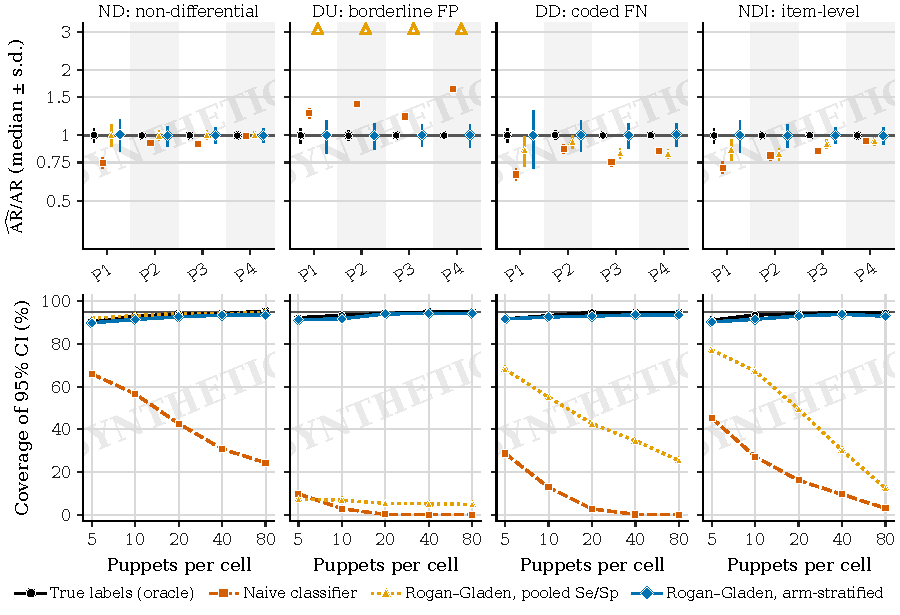
\includegraphics[width=0.94\textwidth]{figures/fig-sim-ar.pdf}
\caption{Synthetic data, E1: estimation of $\mathrm{AR}$ relative to the reverse-chronological reference ($R=1{,}000$ audits per configuration). Top: estimate divided by the true $\mathrm{AR}$, median $\pm$ one Monte Carlo s.d., with $20$ puppets per persona--arm cell; open triangles on the upper edge mark medians beyond the axis (pooled correction under DU, medians $3.4$ to $31$). Bottom: coverage of nominal $95\%$ intervals, averaged over personas, against puppets per cell. ND: non-differential; DU: borderline false positives; DD: coded false negatives; NDI: rates of ND, deterministic per item.}\label{fig:sim-ar}
\end{figure}

\begin{table}[tb]
\centering
\caption{Synthetic data, E1: amplification ratio relative to the reverse-chronological reference, with $20$ puppets per persona--arm cell ($R=1{,}000$; validation of $500$ impressions per arm). Truth: $\mathrm{AR}$ of the pools; it differs between regimes because the avoid-on-flag rule uses the classifier. AR: median estimate. Bias: median relative bias (\%). Cov.: coverage of the nominal $95\%$ interval (\%; MCSE at most $1.6$). RG: Rogan--Gladen correction, error rates pooled over arms or stratified by arm. For the general persona under DU the pooled correction is defined in only $421$ of $1{,}000$ audits, because the corrected reference exposure is otherwise not positive; its median is over those, and the others count as misses.}\label{tab:sim-main}
\footnotesize
\setlength{\tabcolsep}{2.8pt}
\simfit{% Generated by code/make_figures.py from results/sim_results.json -- do not edit by hand.
% E1, reference = chron, 20 puppets per persona-arm cell, validation n = 500 impressions per cell (5 score bands), R = 1000 audits per configuration.
% Truth: pool AR of the regime (regimes differ slightly because the avoid-on-flag choice rule uses the
% classifier). AR: median estimate; Bias: median relative bias (%); Cov.: coverage of the nominal 95%
% interval for AR (%).
\begin{tabular}{@{}llrrrrrrrrrrrr@{}}
\toprule
 & & \multicolumn{3}{c}{P1} & \multicolumn{3}{c}{P2} & \multicolumn{3}{c}{P3} & \multicolumn{3}{c}{P4} \\
\cmidrule(lr){3-5} \cmidrule(lr){6-8} \cmidrule(lr){9-11} \cmidrule(lr){12-14}
Classifier error & Estimator & AR & Bias & Cov. & AR & Bias & Cov. & AR & Bias & Cov. & AR & Bias & Cov. \\
\midrule
Non-differential & Truth & \multicolumn{3}{c}{1.79} & \multicolumn{3}{c}{1.33} & \multicolumn{3}{c}{1.67} & \multicolumn{3}{c}{1.04} \\
 & True & 1.80 & $+$0.2 & 94 & 1.33 & $-$0.2 & 94 & 1.67 & $+$0.0 & 95 & 1.04 & $-$0.2 & 93 \\
 & Naive & 1.34 & $-$25.3 & 0 & 1.23 & $-$7.7 & 50 & 1.52 & $-$8.9 & 27 & 1.04 & $-$0.4 & 94 \\
 & RG pooled & 1.80 & $+$0.4 & 96 & 1.33 & $+$0.0 & 94 & 1.67 & $+$0.2 & 94 & 1.05 & $+$0.3 & 93 \\
 & RG stratified & 1.81 & $+$0.9 & 92 & 1.33 & $-$0.3 & 92 & 1.67 & $+$0.2 & 93 & 1.04 & $-$0.1 & 94 \\
\addlinespace
Differential: borderline FP & Truth & \multicolumn{3}{c}{1.62} & \multicolumn{3}{c}{1.15} & \multicolumn{3}{c}{1.38} & \multicolumn{3}{c}{0.89} \\
 & True & 1.62 & $-$0.0 & 95 & 1.15 & $-$0.3 & 94 & 1.38 & $-$0.1 & 94 & 0.88 & $-$0.1 & 94 \\
 & Naive & 2.05 & $+$26.8 & 0 & 1.61 & $+$39.7 & 0 & 1.69 & $+$22.2 & 0 & 1.45 & $+$63.8 & 0 \\
 & RG pooled & 31.35 & $>{+}10^3$ & 21 & 4.39 & $+$281.6 & 0 & 4.72 & $+$241.8 & 0 & 3.39 & $+$282.8 & 0 \\
 & RG stratified & 1.62 & $+$0.3 & 93 & 1.15 & $-$0.4 & 94 & 1.38 & $+$0.3 & 95 & 0.89 & $+$0.4 & 95 \\
\addlinespace
Differential: coded FN & Truth & \multicolumn{3}{c}{1.82} & \multicolumn{3}{c}{1.36} & \multicolumn{3}{c}{1.78} & \multicolumn{3}{c}{1.07} \\
 & True & 1.82 & $+$0.1 & 95 & 1.36 & $+$0.3 & 94 & 1.78 & $-$0.1 & 94 & 1.07 & $+$0.2 & 95 \\
 & Naive & 1.20 & $-$34.0 & 0 & 1.17 & $-$13.7 & 10 & 1.34 & $-$24.7 & 0 & 0.90 & $-$15.5 & 1 \\
 & RG pooled & 1.55 & $-$14.5 & 80 & 1.27 & $-$6.5 & 83 & 1.47 & $-$17.3 & 6 & 0.88 & $-$17.9 & 2 \\
 & RG stratified & 1.82 & $-$0.1 & 91 & 1.36 & $+$0.4 & 93 & 1.78 & $+$0.2 & 93 & 1.08 & $+$1.0 & 95 \\
\addlinespace
Non-diff. by type, item-level & Truth & \multicolumn{3}{c}{1.82} & \multicolumn{3}{c}{1.30} & \multicolumn{3}{c}{1.69} & \multicolumn{3}{c}{1.03} \\
 & True & 1.82 & $-$0.2 & 94 & 1.30 & $-$0.0 & 95 & 1.69 & $+$0.1 & 94 & 1.03 & $-$0.1 & 94 \\
 & Naive & 1.29 & $-$29.0 & 0 & 1.05 & $-$19.3 & 1 & 1.43 & $-$15.1 & 2 & 0.97 & $-$5.5 & 61 \\
 & RG pooled & 1.57 & $-$13.9 & 70 & 1.07 & $-$17.8 & 12 & 1.54 & $-$8.8 & 49 & 0.97 & $-$6.0 & 67 \\
 & RG stratified & 1.83 & $+$0.4 & 93 & 1.30 & $-$0.3 & 92 & 1.69 & $-$0.0 & 94 & 1.02 & $-$0.4 & 93 \\
\bottomrule
\end{tabular}
}
\end{table}

\paragraph{The reference is part of the estimand} Under ND, $\mathrm{AR}$ is $1.79$, $1.33$, $1.67$ and $1.04$ for the general, Jewish-interest, Middle East and conspiracy-adjacent personas relative to the reverse-chronological feed. It is $2.64$, $1.76$, $2.17$ and $1.29$ relative to the random feed, and $2.76$, $2.05$, $1.17$ and $1.16$ relative to the popularity-only feed, so the ranking of personas changes with the reference (\cref{sec:est-reference}). With true labels, intervals cover in $93.2$--$95.3\%$ of audits with $20$ puppets per cell and in $89.8$--$93.1\%$ with five.

\paragraph{Non-differential error} The naive ratio is attenuated toward one by $25.3\%$, $7.7\%$, $8.9\%$ and $0.4\%$, as \cref{thm:misclass}(a) predicts. The bias does not shrink with more puppets, so coverage falls as the audit grows (general persona: $25.5\%$ with five puppets, $0.0\%$ with $20$). Both corrections have median biases below $1\%$ and coverage of $91.8$--$95.6\%$.

\paragraph{Differential error} For the general persona the algorithm shows more borderline content than the reverse-chronological feed ($11.2\%$ against $3.0\%$ of impressions) and a larger coded share of antisemitic content ($63\%$ against $48\%$). Its specificity is therefore lower under DU and its sensitivity under DD, although no type is classified differently by arm. Under DU the naive ratio is biased upward by $22$--$64\%$, and for the conspiracy-adjacent persona it turns a true $0.89$ into $1.45$. The pooled correction is worse. It subtracts a false-positive rate that is too large for the reference arm, which drives the corrected reference exposure toward zero. For the general persona that exposure was not positive in $579$ of $1{,}000$ audits, and elsewhere the median ratio was $31.3$ against a truth of $1.62$. Under DD the naive ratio is biased by $-14$ to $-34\%$, and for the conspiracy-adjacent persona the naive ($0.90$) and pooled ($0.88$) ratios put a true $1.07$ below one, as in scenario A of \cref{tab:mc-signflip}. The coverage of the pooled correction falls as the audit grows, to $0\%$ for two personas with $80$ puppets. Under NDI each item is always classified in the same way, so an arm's sensitivity depends on which antisemitic items it shows ($0.69$ against $0.79$ for the Jewish-interest persona). Error that is non-differential type by type is then differential by arm, and the naive and pooled ratios are biased by up to $-29.0\%$ and $-17.8\%$. In all three regimes, correction by arm has median biases within $1\%$ and coverage of $90.7$--$95.2\%$.

\paragraph{The price of stratifying} With five puppets per cell, the stratified correction's standard errors are $82$--$94\%$ of the Monte Carlo s.d., and its coverage $88.1$--$94.8\%$. Its mean bias reaches $5.6\%$ because the ratio is skewed, but its median bias stays within $2.5\%$. Validation by arm, as in the protocol (\cref{sec:protocol}), is the safe default; the pooled correction is not.

\subsection{Variance estimators and closed forms (E1b)}\label{sec:sim-checks}

E1b draws $R=2{,}000$ audits from separate pools that record every session. Error rates are known, or estimated externally from $n_1=300$ coded positives and $n_0=1{,}500$ coded negatives (\cref{tab:sim-checks}, \cref{app:sim-further}). As simulated, sessions of a puppet are nearly uncorrelated (design effects $0.96$--$1.23$) and both variance estimators cover. When accounts sit in different experiment buckets, a persistent random shift in the algorithm's weight on bait, the algorithmic arm's design effect rises to $2.75$--$5.65$. Session-level intervals for $\mathrm{AA}$ then cover in only $62.9$--$82.5\%$ of audits, against $93.0$--$93.2\%$ for cluster-robust ones, as \cref{thm:identify}(c) predicts. The form $\mathrm{AR}\,\kappa_a/\kappa_r$ of \eqref{eq:mc-diff} reproduces every naive ratio, and under DD the limit $\mathrm{AR}^{\mathrm{pool}}$ matches the median pooled correction to within $0.006$ (for the conspiracy-adjacent persona both are $0.861$, below one, although the truth is $1.053$). The delta-method s.d.\ of $\log\widehat{\mathrm{AR}}$ understates when $\kappa_{\Sp}=v_{\Sp}^{1/2}/(J\mu_r)$ is large, as \cref{sec:meas-misclass} warns. With $\kappa_{\Sp}\le0.102$, its median over audits is within $-5.3$ to $+3.9\%$ of the Monte Carlo s.d. For the general persona, whose reference exposure is lowest ($\kappa_{\Sp}=0.246$), it understates by $15$--$23\%$, and by up to $33\%$ under DD ($\kappa_{\Sp}=0.312$). Reporting $\kappa_{\Sp}$ and a bootstrap is therefore warranted.

\subsection{Interference (E2)}\label{sec:sim-interference}

Each audit has $15$ protocol puppets per persona and arm (algorithmic, reverse-chronological, popularity-only) and $8$ untrained sentinels, whose openings feed global popularity. The background volume is set so that the puppets generate a share of $0.02$ to $0.3$ of all openings. The load $\bar\ell$ of \cref{sec:id-interference}, the puppets' share of the engagement with the items they open, is then $0.023$ to $0.331$. Each of $R=24$ replications is run at every share with common random numbers, and the bias is the paired difference from the audit without interference. Puppets draw their seeds from the $40$ items closest to their persona. The remedies are low co-viewing (seeds from $200$ items) and staggered waves (five waves, five days apart). Biases are in units of $10^{-3}$ (\cref{fig:sim-interference}; \cref{tab:sim-designs} in \cref{app:sim-further} summarises E2--E5).

\begin{figure}[tb]
\centering
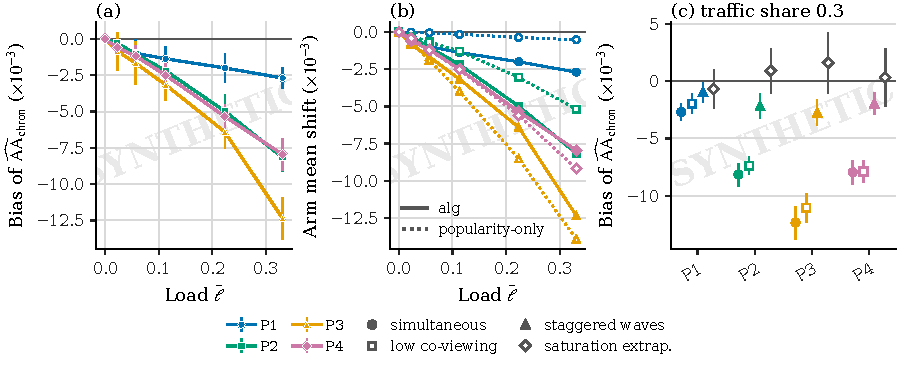
\includegraphics[width=0.94\textwidth]{figures/fig-sim-interference.pdf}
\caption{Synthetic data, E2: interference through shared popularity ($R=24$ paired replications; bars $\pm2$ SE). (a) Bias of the additive amplification relative to the reverse-chronological feed against the load $\bar\ell$, simultaneous design. (b) Shift in mean exposure of the algorithmic arm (solid) and the popularity-only arm (dotted); the reverse-chronological arm does not move. (c) Bias at traffic share $0.3$: simultaneous (load $0.33$), low co-viewing ($0.33$), staggered waves ($0.12$), and randomised-saturation extrapolation from shares $0.1$ and $0.3$.}\label{fig:sim-interference}
\end{figure}

\paragraph{Bias} The bias of $\widehat{\mathrm{AA}}_{\mathrm{chron}}$ is negative for every persona and grows with the load. At share $0.3$ it is $-19$, $-45$, $-23$ and $-247\%$ of the no-audit value, so for the conspiracy-adjacent persona interference reverses the sign of the estimate. Even at share $0.02$ it is $-1.5$ to $-3.5\%$ for three personas and $-19\%$ for the fourth. At share $0.3$, Wald intervals cover in only $25.0$--$70.8\%$ of replications. Exposure under the algorithm and the popularity-only feed falls monotonically with the load, while the reverse-chronological feed, which does not learn, does not move. Avoid-on-flag puppets rarely open antisemitic items, so the popularity they add goes to other items: case (i) of \cref{prop:interference}(b), here over whole sessions. Because the popularity-only feed also learns, the shifts partly cancel. For three personas $\xi_\Delta$ is $0.008$--$0.009$ against that feed and $0.025$--$0.037$ against the reverse-chronological feed.

\paragraph{Remedies} Low co-viewing barely helps, presumably because the seed pool governs only $30$ of a puppet's up to $230$ openings and the first item of each session. Staggering lowers the load to $0.118$ and the bias by $64$--$78\%$. Extrapolating to zero load from shares $0.1$ and $0.3$ (\cref{prop:interference}(c)) leaves biases within $1.2$ SE of zero. It costs $2.3$--$2.8$ times the variance of one audit at share $0.1$, and $4.4$--$5.9$ times for closer loads. The sensitivity interval of \cref{prop:interference}(d), with $\xi_\Delta$ at its simulated value, restores coverage to $95.8$--$100\%$. The breakdown value $\xi^\ast$ is well above the simulated slope only for the Middle East persona ($0.101$ against $0.037$). Sentinel exposure falls by $0.0063$ per unit of load, against $0.0075$--$0.0355$ for the trained algorithmic arms. Sentinels are therefore evidence about $\xi$, not a bound on it.

\subsection{Supply, demand and the fixed-demand audit (E3)}\label{sec:sim-decomp}

The population has $3{,}000$ synthetic users with naturalistic choice and new accounts. Their initial demand $F_0$ is drawn from the four personas (shares $0.6$, $0.1$, $0.15$, $0.15$), with individual noise. Two copies are formed for $H\in\{3,10,20,40\}$ sessions, one under the algorithm and one under the reverse-chronological feed, while demand evolves. Each copy is then evaluated under both policies with demand held fixed, which gives the four cells $\bar\mu(a;b)$ of \cref{thm:decomp} for the same users. The fixed-demand audit holds each user's initial demand fixed in a new account, which is the audit of \cref{prop:audit-scope} at $Q=F_0$.

\begin{figure}[tb]
\centering
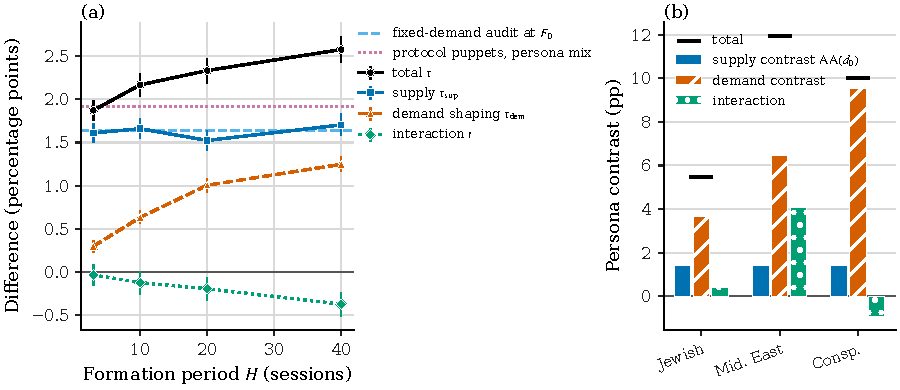
\includegraphics[width=0.94\textwidth]{figures/fig-sim-decomp.pdf}
\caption{Synthetic data, E3: the decomposition of \cref{thm:decomp}. (a) Components for $3{,}000$ synthetic users whose demand evolves, against the length $H$ of the formation period (reference: reverse-chronological; bars $\pm2$ SE over users). Lines: the fixed-demand audit at the initial demand $F_0$, and protocol puppets with the persona mix of the population. (b) Persona-contrast decomposition relative to the general persona $d_0$ (protocol puppets, regime ND); black marks: total $\mu_{\mathrm{alg}}(d)-\mu_{\mathrm{ref}}(d_0)$.}\label{fig:sim-decomp}
\end{figure}

After $40$ formation sessions, the total effect $\tau=2.58$ percentage points (SE $0.08$) splits into supply $\tau_{\mathrm{sup}}=1.70$, demand shaping $\tau_{\mathrm{dem}}=1.25$ and an interaction $\iota=-0.37$ (SE $0.07$). The Shapley shares are $1.52$ and $1.06$, and $\mathrm{TR}=1.45=1.24\times1.17$. As formation lengthens, supply stays between $1.52$ and $1.70$, while demand shaping grows from $0.30$ and the interaction falls from $-0.04$ (\cref{fig:sim-decomp}(a)). The algorithm adds less to demand that it has formed: after $40$ sessions its users draw $7.2\%$ of their pool from borderline and antisemitic sources, against $3.6\%$ under the reference, and the reverse-chronological feed shows those sources too. \Cref{asm:demand} holds closely: no cell differs from fixed-demand accounts with the same demand by more than $0.11$ points (SE $0.05$). The fixed-demand audit gives $\mathrm{AA}=1.64$ points, close to the supply effect. It falls short of the total by $0.23$ points at $H=3$ and by $0.94$ (SE $0.07$) at $H=40$, as \cref{prop:audit-scope} says it must. In the persona contrasts (\cref{fig:sim-decomp}(b)), demand contrasts dominate, but they compare scripts that we chose, not demand formed by the algorithm. The rates at which taste, appetite and follows change are invented. The sizes of $\tau_{\mathrm{dem}}$ and $\iota$, and the sign of $\iota$, belong to these dynamics. E3 shows what a fixed-demand audit targets, not how real demand evolves.

\subsection{Markov predictions and sensitivity (E4)}\label{sec:sim-markov}

For each persona and policy, $250$ naturalistic accounts with fixed demand, which always open an item, run three burn-in sessions. A chain over the states $N$, $B$ and $A$ of the opened items is then estimated from $10$ sessions of $20$ steps (\cref{prop:markov-mle}). It is compared with the same sessions ($e_{20}$), with one further session of $200$ steps ($e_{200}$), and, for $\varpi(\mathcal A)$, with that session's second half. Exposure here counts consumed items.

\begin{figure}[tb]
\centering
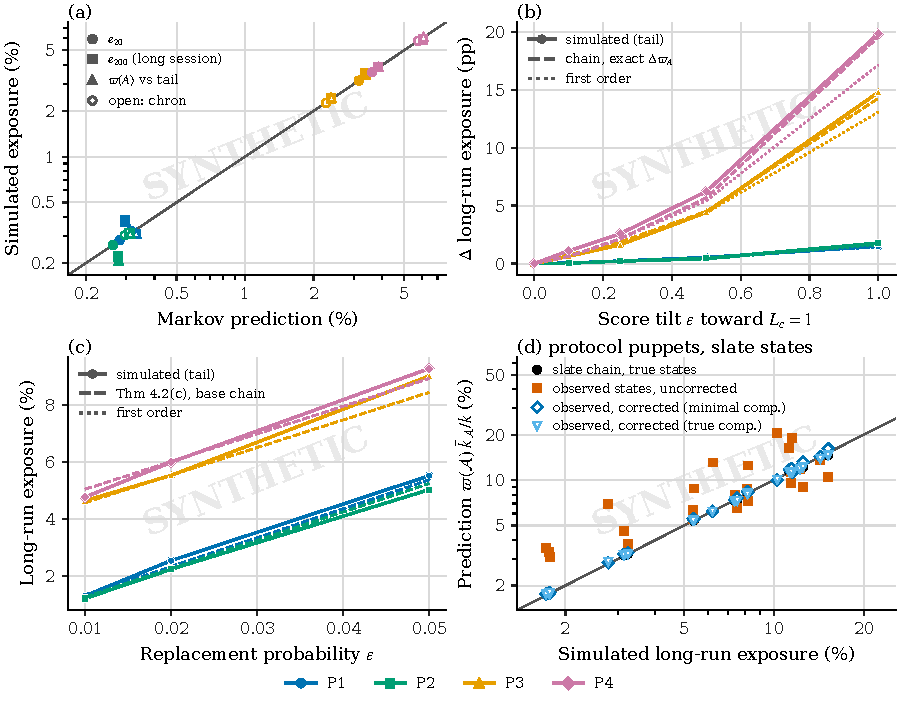
\includegraphics[width=0.94\textwidth]{figures/fig-sim-markov.pdf}
\caption{Synthetic data, E4: Markov chains of consumed items ($250$ accounts per persona and policy). (a) Predictions against simulation for $e_{20}$, $e_{200}$, and $\varpi(\mathcal A)$ against the second half of a $200$-item session; open markers: reverse-chronological. (b) Score tilt $\varepsilon$ toward items with $L_c=1$: simulated change in long-run exposure, the exact change between the estimated chains (\cref{thm:perturb}(a)), and its first-order term. (c) Replacement of the next item by an antisemitic one with probability $\varepsilon$: simulation, the closed form of \cref{thm:perturb}(c) from the base chain alone (dashed), and its first-order term $\varpi(\mathcal A)(1+\varepsilon\,\E_\varpi\tau_A)$ (dotted).}\label{fig:sim-markov}
\end{figure}

The chain reproduces $e_{20}$ within $0.0002$ in all eight cells, which is an in-sample check. Out of sample, $e_{200}$ is predicted within $7\%$ in six cells. It errs by $-22\%$ and $+26\%$ in the algorithmic arms of the general and Jewish-interest personas, where exposure is rarest (about $0.3\%$) and $\varpi(\mathcal A)$ misses the second-half share by up to $34\%$. At the audited horizon, session averages should remain primary (\cref{sec:markov-estimation}). The chains mix fast: Kemeny's constant is $1.98$--$2.17$ and $\kappa_{\mathcal A}$ is $0.50$--$0.52$ in every cell. This world therefore lacks the sticky regions in which \cref{thm:perturb} predicts the largest magnifications. When the algorithm's score of antisemitic items is tilted, the exact identity of \cref{thm:perturb}(a), applied to the estimated chains, tracks the simulated change (at $\varepsilon=1$, $14.26$ against $14.77$ percentage points for the Middle East persona). The bound of part (b) holds but is loose. It exceeds the exact change by factors of $1.3$--$3.3$ for the Middle East and conspiracy-adjacent personas and $3.2$--$120$ for the other two, because $\|P_1-P_0\|_\infty$ includes the rarely visited, noisily estimated row of $A$. When the next item is replaced by an antisemitic one with probability $\varepsilon\le0.05$, the closed form of \cref{thm:perturb}(c), computed from the base chain alone, predicts long-run exposure within $9\%$. Its multiplier shows. For the general persona, with $\E_\varpi\tau_A=345$ items, replacing $1\%$ of items raises long-run exposure from $0.31\%$ to $1.30\%$. For the Middle East persona, which reaches antisemitic items quickly anyway, it rises from $3.56\%$ to $4.64\%$.

\subsection{The sequential audit (E5)}\label{sec:sim-sequential}

Pairs of one algorithmic and one reverse-chronological puppet are resampled from the E1 pools (regimes ND and DD) and arrive in waves of five. Each puppet codes $m=10$ flagged positions, giving $Y_u=\bar Q_u\widehat P_u$, and \cref{alg:sequential} runs with the mixture tuned to $t^\ast=40$ pairs. There are $R=2{,}000$ audits of up to $400$ pairs ($80$ waves) per configuration. In the null case both arms come from the reference pool. The sensitivity ratio is $\lambda_S=1.00$ under ND, and $0.86$, $0.93$, $0.83$ and $0.82$ under DD. Stopping is evaluated at the settings for which the protocol was first written: $\alpha=0.0125$ per persona, $\delta=1.25$, $b=1$ burn-in wave, and $W_{\max}=8$ waves of five pairs. \Cref{sec:protocol} explains why the registered design is larger.

\begin{figure}[tb]
\centering
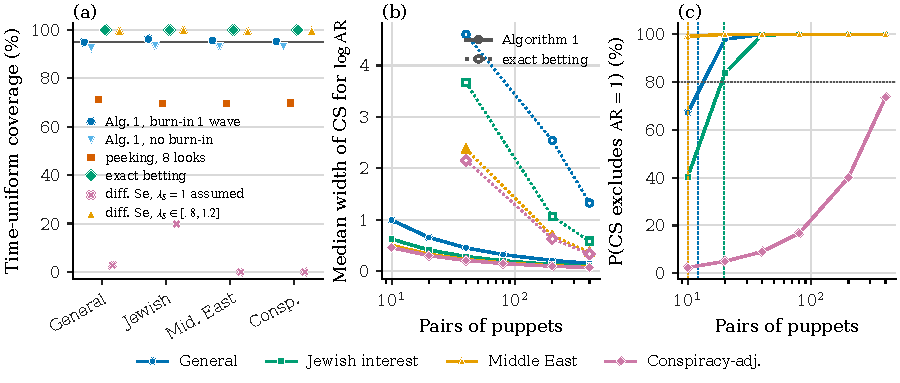
\includegraphics[width=0.94\textwidth]{figures/fig-sim-sequential.pdf}
\caption{Synthetic data, E5: \cref{alg:sequential} against the reverse-chronological reference, waves of five pairs ($R=2{,}000$; exact betting $R=200$). (a) Time-uniform coverage at $\alpha=0.05$ over $80$ waves, with and without one burn-in wave; a fixed-sample interval recomputed after each of the first eight waves (peeking); exact betting; and, under DD, $\lambda_S=1$ assumed or the range $[0.8,1.2]$. (b) Median width for $\log\mathrm{AR}$: \cref{alg:sequential} (solid), exact betting (dotted). (c) Probability of excluding $\mathrm{AR}=1$; dashed verticals: the horizon $n_{\mathrm{seq}}$ of \cref{prop:power}(d), at least two waves (beyond the axis for the conspiracy-adjacent persona).}\label{fig:sim-sequential}
\end{figure}

\paragraph{Coverage and peeking} With one burn-in wave, time-uniform coverage over $80$ waves at $\alpha=0.05$ is $95.0$--$96.2\%$, and $95.0$--$96.3\%$ under the null. Without it, coverage is $92.6$--$93.5\%$ and $92.0$--$94.0\%$: the first wave, with five pairs and a skewed $Y_u$, is where the normal approximation fails (\cref{sec:meas-sequential}). At $\alpha=0.0125$ (nominal $98.75\%$), coverage is $98.0$--$98.8\%$ with the burn-in and $96.0$--$97.0\%$ without, so the relative excess of the miss rate is largest at the per-persona level. A fixed-sample interval recomputed after each of the first eight waves covers at every look in only $69.5$--$71.2\%$ of audits. Under the null it rejects $\mathrm{AR}=1$ at some look in $29.2$--$33.0\%$ of audits, against $2.1$--$3.4\%$ for \cref{alg:sequential}. Most of the excess over the $17.6\%$ of \cref{sec:meas-sequential} comes from the first look.

\paragraph{Conclusions on the original budget} Under ND, the audit contradicts the true $\mathrm{AR}$ in at most $0.05\%$ of audits. It concludes material amplification for the general persona ($\mathrm{AR}=1.79$) in $85.8\%$ of audits, after $5.1$ waves on average, and for the Middle East persona ($1.67$) in $99.9\%$, after $2.8$. It concludes no material difference for the conspiracy-adjacent persona ($1.04$) in $91.2\%$. For the Jewish-interest persona, whose ratio of $1.33$ lies just above $\delta=1.25$, it detects a difference by wave $8$ in $98.7\%$ of audits, but materiality stays undetermined in $93.8\%$ within the eight-wave budget, and in $64.1\%$ even after $40$ waves. Under the null, wrong conclusions occur in $0.20$--$1.05\%$ of audits with the burn-in, within the per-persona level of $1.25\%$, and in up to $2.95\%$ without it.

\paragraph{Power} The closed form $A_Y$ of \cref{prop:power}(d) overstates the simulated variance by $5$--$23\%$, which is conservative. The simulated power for detecting $\mathrm{AR}\ne1$ is $0.82$--$0.93$ at $n_{\mathrm{fix}}$ and $0.85$--$1.00$ by $n_{\mathrm{seq}}$ (\cref{tab:sim-designs}). With $\lambda_S\in[0.95,1.05]$, no horizon exists for the conspiracy-adjacent persona, since $|\log\mathrm{AR}|=0.042<\log(1.05/0.95)$. The exact betting sequence covers in all $200$ of its audits but is nearly powerless here: its median width at $40$ pairs is $2.2$--$4.6$, against $0.21$--$0.45$ for \cref{alg:sequential}.

\paragraph{Differential sensitivity} Under DD, assuming $\lambda_S=1$ gives coverage of $2.8$, $19.8$, $0.0$ and $0.0\%$, because the sequence then covers $\lambda_S\mathrm{AR}$, not $\mathrm{AR}$. For the conspiracy-adjacent persona ($\mathrm{AR}=1.07$, $\lambda_S\mathrm{AR}<1$), the audit detects de-amplification within eight waves in $48.5\%$ of audits. The range $[0.8,1.2]$, which contains every $\lambda_S$ of the regime, restores coverage to $99.4$--$100\%$ and removes the wrong conclusions, but takes most of the power with them. By wave $8$ the sequence excludes $\mathrm{AR}=1$ in $49.6$, $5.5$, $92.8$ and $0.0\%$ of audits, against $96.1$, $85.0$, $100$ and $54.8\%$ with $\lambda_S=1$.

\subsection{What the simulation does and does not show}\label{sec:sim-scope}

Where their conditions hold, the results of \cref{sec:estimands,sec:markov,sec:identification,sec:measurement} hold in finite samples: corrections by arm, cluster-robust intervals, the closed forms of \cref{thm:misclass,thm:perturb}, the scope of fixed-demand audits (\cref{prop:audit-scope}), and \cref{alg:sequential} with one burn-in wave at $\alpha=0.05$. The methods also fail where the theory says they will. Error that depends only on content still differs between arms, and then the naive ratio and the pooled correction can lie on the wrong side of one. The pooled correction explodes when the corrected reference exposure nears zero. Interference can reverse the sign of the additive amplification. Assuming $\lambda_S=1$ under differential sensitivity gives $0$--$20\%$ coverage, and a declared range that contains $\lambda_S$ restores it, at the cost of power. Approximations show at these sizes. The miss rate of \cref{alg:sequential} reaches $2.0\%$ against $1.25\%$ at the per-persona level, the delta-method s.d.\ understates when $\kappa_{\Sp}$ is large, Markov extrapolation to long sessions errs by up to $26\%$, and the bound of \cref{thm:perturb}(b) is loose. On the original eight-wave budget, materiality stays undetermined for the persona whose ratio lies near the margin.

The simulation does not show how any real recommender behaves. The world, the classifier, the personas and the demand dynamics are invented, and the ratios from $0.89$ to $2.76$, the interference biases and the decomposition shares follow from our parameters. Parts of the protocol were not simulated. E5 evaluates \cref{alg:sequential} on the confirmed-flagged statistic, with pairs resampled independently from fixed pools: no drift, interference, attrition or coder error. It uses ten sessions and slates of four, and it evaluates neither the sequence on double-sampled exposures nor the sample sizes of the registered design (\cref{sec:protocol}). E4 models the opened items of naturalistic accounts, not the slate states of the protocol, and its fast-mixing chains do not test the sticky regime. E2 has one interference channel, $24$ replications, and no load below $0.023$. E3 rests on dynamics of demand for which we have no evidence. And because puppets and users are served by the same rules by construction, the transport condition (\cref{asm:id-transport}), which a real audit can least check, is never at risk.
}{}
\IfFileExists{sections/08-protocol.tex}{\section{A pre-registered audit protocol}\label{sec:protocol}

This section is the protocol we will register, time-stamped and with the commit hash of the analysis code and the classifier version, before any audit account is created or any session is run \citep{nosek2018}. It commits in advance to the service and surface, the personas, the randomisation, the interference controls, the validation design, the estimands, the stopping and decision rules, and the handling of data. Any departure will be reported as a deviation, with its reason. The estimators are those of \cref{sec:identification,sec:measurement}, evaluated on synthetic data in \cref{sec:simulation}. The protocol is written for a generic service. It names no platform, and it contains no results. The ethical and legal conditions it depends on are set out in \cref{sec:ethics}, and no step below is taken unless those conditions are met.

\subsection{Service, surface and access route}\label{sec:prot-scope}

The unit of audit is one recommendation \emph{surface} (for example a home feed, or a list of items recommended next to the current one) of one service, in one jurisdiction, during one audit window. The service and surface are chosen at registration by three criteria, in this order:
\begin{enumerate}[(i)]
  \item \emph{A reference policy is available.} AR and AA require exposure under a reference policy $\pi=\mathrm{ref}$ (\cref{def:amplification}). On a live service, the candidates are the non-profiling option that very large online platforms must offer under Article~38 of the DSA, or a reverse-chronological option where offered (\cref{sec:bg-governance}), and logged-out sessions (\cref{sec:bg-debates}). The random-from-eligible-pool and popularity-only reference policies of \cref{def:amplification} are not generally available to an outside auditor. They are evaluated in \cref{sec:simulation}, and on a live service only if data obtained under Article~40(4) permit it. If no reference policy is available for a surface, we report exposure under the algorithmic policy and the Markov summaries of \cref{prop:markov} for that surface, and no amplification estimate.
  \item \emph{A lawful access route exists.} In order of preference: data obtained as a vetted researcher under Article~40(4) of the DSA, or through a research interface the provider offers, where these can deliver exposure under a fixed demand profile; access to publicly accessible data under Article~40(12); and a sock-puppet audit only where neither route can identify the estimand, and only after the legal review and ethics approval of \cref{sec:ethics}.
  \item \emph{The classifier is validated for the content.} The service's dominant language(s) and formats (text, images, video transcripts) must be covered by the frozen classifier and by the annotators of \cref{sec:prot-validation}.
\end{enumerate}
The jurisdiction is an EU Member State, so that the DSA routes apply and the Article~38 option is in scope. All puppets present from that jurisdiction.

\subsection{Personas, puppets and sessions}\label{sec:prot-personas}

\paragraph{Personas}
A persona $d\in\mathcal D$ is a demand profile. It has three components: a pool of seed items used to train the account; a choice rule that selects one item from each slate; and an interaction budget. The candidate set has four personas. Their seed pools are compiled and screened before registration, and two coders confirm that no seed item is antisemitic under the codebook of \cref{sec:prot-validation}.
\begin{enumerate}[(a)]
  \item \emph{General interest} ($d_0$, the baseline): mainstream news, sport, entertainment and how-to content.
  \item \emph{Jewish interest}: Jewish culture, religion, history and community news. Users who seek such content may be targeted by antisemitic replies and recommendations, so this persona measures what the algorithm supplies to an audience that is often the target of the content.
  \item \emph{Middle East news}: news and commentary on Israel, the Palestinian territories and the region, drawn from a seed pool balanced across outlets and viewpoints by two coders working independently.
  \item \emph{Conspiracy-adjacent}: content on conspiracy theories about elites, finance or health that is not itself antisemitic under the codebook. This is the persona whose demand lies closest to antisemitic content without requiring any engagement with it.
\end{enumerate}
No persona is trained on antisemitic content. A persona that sought it out would inflate the engagement metrics of hateful items, which the protocol forbids (\cref{sec:eth-footprint}). The audit therefore asks what each policy \emph{supplies} to profiles whose demand is legitimate or adjacent, not what it delivers to users who seek antisemitic content.

\paragraph{Choice rule and the avoid-on-flag constraint}
At each step $t$ the puppet observes a slate. Every item in the first $k$ positions is recorded and scored by the frozen classifier. The puppet then opens the highest-ranked item whose classifier score is below a registered threshold $\tau_{\mathrm{safe}}$ and whose similarity to the persona's seed pool exceeds a registered threshold. If no item meets both conditions, it opens the highest-ranked item below $\tau_{\mathrm{safe}}$. Items scoring above $\tau_{\mathrm{safe}}$ are recorded as exposures but never opened. The choice rule is part of the persona, so it is applied identically under both policies. AR$(d)$ is then defined conditional on it. Because the rule depends on the classifier, false negatives can still be opened. Their number is estimated from the validation sample and reported as the residual footprint (\cref{sec:eth-footprint}).

\paragraph{Exposure}
Exposure $E_u(\pi)$ is computed as in \cref{def:amplification}, averaging over the first $k$ slate positions at each of the $T$ steps of a session and over a puppet's measurement sessions. With $k=1$ it reduces to the top-ranked item. The registered $k$ is the number of items visible without scrolling on the surface's default layout, fixed during the pilot.

\paragraph{Session structure}
Each puppet passes through a \emph{training phase} and a \emph{measurement phase}. In training, it opens a random subset of its persona's seed pool, one session per day for $D_{\mathrm{train}}$ days, with a fixed dwell time per item. Drawing a different random subset for each puppet limits the overlap in viewing between puppets of the same persona, which is a channel of interference (\cref{sec:prot-interference}). In measurement, it runs $S$ sessions, at most one per day at a randomised time, each of $T$ steps, starting from a registered entry point (the home surface, or a seed item drawn at random from the pool). \Cref{tab:prot-design} gives the design parameters. The values are candidates. The puppet counts are fixed at registration by \cref{prop:power}, and the other values by the pilot.

\begin{table}[tbp]
\centering
\caption{Design parameters of the audit. Candidate values are illustrative and are fixed at registration as indicated; none is a result.}\label{tab:prot-design}
\footnotesize
\setlength{\tabcolsep}{4pt}
\renewcommand{\arraystretch}{1.15}
\begin{tabularx}{\textwidth}{@{}>{\raggedright\arraybackslash}p{4.3cm}>{\raggedright\arraybackslash}p{2.4cm}>{\raggedright\arraybackslash}X@{}}
\toprule
Parameter & Candidate & Fixed by \\
\midrule
Personas $|\mathcal D|$ & 4 & Registration (\cref{sec:prot-personas}) \\
Policy arms & alg, ref & Reference policy available on the surface (\cref{sec:prot-scope}) \\
Puppets per persona--arm cell per wave & 5 & \Cref{prop:power} with pilot inputs \\
Maximum number of waves $W_{\max}$ & 8 & \Cref{prop:power}; budget and footprint cap \\
Training days $D_{\mathrm{train}}$; seeds opened per day & 3; 10 & Pilot (stability of recommendations) \\
Measurement sessions $S$ per puppet & 10 & Pilot (within-puppet correlation) \\
Steps per session $T$; positions recorded $k$ & 20; visible slate & Pilot; surface layout \\
Sentinel (untrained) puppets per wave & 2 & Fixed \\
Validation sample (items) & 2,000 & Precision of $\widehat{\mathrm{Se}}$, $\widehat{\mathrm{Sp}}$ per arm (\cref{sec:prot-validation}) \\
Overall error level $\alpha$; material-difference margin $\delta$ & 0.05; 1.25 & Registration (\cref{sec:prot-stopping}) \\
\bottomrule
\end{tabularx}
\end{table}

\subsection{Randomisation}\label{sec:prot-randomisation}

All accounts are created in the same way, before any is assigned, so that features of account creation cannot differ systematically by arm. The audit runs in waves $w=1,\dots,W$ that start on different days. Within each wave, puppets are assigned completely at random to the $|\mathcal D|\times 2$ persona--policy cells in equal numbers. Persona training is therefore randomised, and policy is randomised independently of it. Seed subsets, session start times and the order in which puppets run within a day are also randomised. All puppets are trained in the same way whatever their arm. The policy contrast is applied only at the start of the measurement phase: puppets in the reference arm switch to the non-profiling or chronological option, or run their measurement sessions logged out with the same choice rule. Training is thus identical in distribution across arms, and the only systematic difference at measurement is the policy. This is the design whose identification conditions are stated in \cref{thm:identify}. Waves are blocks. Because every wave contains every cell, a change in the service's policy during the audit window affects both arms of a wave equally, and the blocked analysis of \cref{sec:identification} separates such drift from amplification. Known changes announced by the service during the window are logged as they occur.

\subsection{Interference controls}\label{sec:prot-interference}

Puppets share the learning system they audit. Through it, one puppet's behaviour can change what another is shown, which violates the no-interference condition of \cref{thm:identify}. The protocol limits interference by design, and it measures what remains so that the bound of \cref{prop:interference} can be applied with an estimated $\xi$.
\begin{itemize}
  \item \emph{Isolation.} Puppets never follow, message, mention or otherwise interact with any account, including each other. Each runs in its own browser profile with separate storage, and no identifier is shared between puppets.
  \item \emph{Limited co-viewing.} Each seed item may be opened by at most a registered number of puppets per wave. Seed subsets are drawn so that puppets of the same persona overlap as little as the pool allows.
  \item \emph{Staggered start.} Waves start on different days, and a wave's puppets start their sessions at randomised times. This limits the number of puppets active at once, which is the quantity the interference bound depends on.
  \item \emph{Device and network hygiene.} Each puppet keeps one consistent device profile and one stable network location within the study jurisdiction for its whole life. Network locations are not rotated to evade a service's detection or rate limits, and no technical access control is circumvented (\cref{sec:eth-legal}). A puppet that is challenged, restricted or suspended is stopped and not replaced within the wave. Its attrition and the reason are recorded, and attrition is compared across arms.
  \item \emph{Sentinels.} In each wave, a few untrained puppets run measurement sessions under the algorithmic policy. Their exposure should not depend on the number of trained puppets active at the same time. The registered test of that dependence gives the estimate of $\xi$ used in \cref{prop:interference}. Sentinels also track drift across waves.
\end{itemize}

\subsection{Classifier and validation sample}\label{sec:prot-validation}

\paragraph{Frozen classifier}
The classifier follows the lab's detection proposal \citep{kornsteinlab2026detection}. Its version, decision threshold and $\tau_{\mathrm{safe}}$ are fixed and hashed at registration and are not changed during the audit. Every recorded item receives a score; $\widehat L_c$ is the thresholded score.

\paragraph{Sampling}
The validation sample is drawn from the distinct recorded items, stratified by policy arm, persona and classifier-score band (five bands). High-score bands are oversampled, and within strata the allocation follows the Neyman rule using pilot variances \citep{neyman1934}, with a registered minimum per stratum. Each stratum contains both flagged and unflagged items, so that sensitivity and specificity are estimable separately in each arm. This is required because classifier error may differ by arm when the content mix differs (\cref{thm:misclass}). Items are sampled after each wave, which lets the validation data grow with the audit, and are weighted by the inverse of their inclusion probabilities.

\paragraph{Coding}
Two trained annotators code each sampled item independently. They are blind to arm, persona and classifier score, and work from a written codebook. The codebook has four primary categories: \emph{antisemitic} (including coded forms); \emph{quotes, reports or criticises antisemitism}; \emph{borderline or ambiguous}; and \emph{not antisemitic}. It also has a flag for content concerning Israel or Zionism. The primary label is $L_c=1$ for the first category only. Sensitivity analyses count borderline items as antisemitic, and report scope variants under the IHRA and JDA definitions where they differ \citep{ihra2016,jda2021}, side by side and without a preferred variant. A third, senior coder adjudicates disagreements; items are not dropped. Annotators complete a calibration round on items outside the audit until their agreement reaches a registered threshold. Agreement is reported as Cohen's $\kappa$ \citep{cohen1960}, overall and by stratum. Coders must be fluent in the languages of the items. The protections for annotators are those of \cref{sec:eth-annotators}.

\paragraph{Use}
The adjudicated labels give weighted estimates of sensitivity and specificity by arm. These enter the Rogan--Gladen-type correction \citep{rogangladen1978} and the delta-method variance of \cref{thm:misclass}. We report a test of equal error rates across arms, and corrected and naive estimates side by side.

\subsection{Pre-registered estimands and analysis}\label{sec:prot-estimands}

\paragraph{Primary}
For each persona $d\in\mathcal D$, the misclassification-corrected amplification ratio $\mathrm{AR}(d)$ and additive amplification $\mathrm{AA}(d)$ of \cref{def:amplification}, comparing the algorithmic policy with the registered reference policy, identified under the conditions of \cref{thm:identify}.

\paragraph{Secondary}
\begin{enumerate}[(i)]
  \item The supply/demand decomposition of \cref{thm:decomp} for each persona $d$ relative to the baseline persona $d_0$, including its interaction term. The demand contrast is the difference between personas under the reference policy; the supply contrast is the difference between policies for the baseline persona.
  \item Markov exposure summaries (\cref{prop:markov}): transition matrices $P_{\mathrm{alg}}$ and $P_{\mathrm{ref}}$ over the content states neutral, borderline and antisemitic, estimated from step-to-step transitions of the opened items and corrected for misclassification; the implied stationary exposure, expected hitting times of the antisemitic state, and the sensitivity of stationary exposure given by \cref{thm:perturb}. These are model-based and are reported as such.
  \item Diagnostics: the interference estimate $\xi$ and its bound (\cref{prop:interference}); drift across waves from sentinels and blocks; attrition by arm; equality of error rates across arms.
\end{enumerate}

\paragraph{Exploratory}
Exposure by slate position, and heterogeneity by entry point.

\subsection{Sequential monitoring, stopping and decision rules}\label{sec:prot-stopping}

After each wave, a confidence sequence for $\log\mathrm{AR}(d)$ is updated for every persona by \cref{alg:sequential}, at level $1-\alpha/|\mathcal D|$ per persona so that the family of sequences has simultaneous coverage $1-\alpha$. Confidence sequences are valid at arbitrary stopping times \citep{howard2021,ramdas2023}. Stopping early when the evidence is clear therefore does not inflate error rates, as repeated fixed-sample tests would; the idea goes back to Wald's sequential tests \citep{wald1945}. Early stopping also reduces the footprint of the audit (\cref{sec:eth-footprint}). For each persona, data collection stops at the first wave at which one of the following holds:
\begin{enumerate}[(S1)]
  \item the confidence sequence lies entirely above $\log\delta$ or entirely below $-\log\delta$ (a material difference in one direction);
  \item the confidence sequence lies entirely within $(-\log\delta,\log\delta)$ (no material difference);
  \item the wave budget $W_{\max}$ is reached.
\end{enumerate}
A persona whose cells stop no longer receives puppets in later waves. The other personas continue. At the end, the conclusion for each persona is stated according to \cref{tab:prot-decisions}. Every persona is reported, whatever its result.

\begin{table}[tbp]
\centering
\caption{Registered decision rules for persona $d$, based on the final confidence sequence for $\mathrm{AR}(d)$, with margin $\delta$; the first matching row applies. Each conclusion is stated for the audited service, surface, jurisdiction, window and persona only.}\label{tab:prot-decisions}
\footnotesize
\renewcommand{\arraystretch}{1.15}
\begin{tabularx}{\textwidth}{@{}>{\raggedright\arraybackslash}p{5.2cm}>{\raggedright\arraybackslash}X@{}}
\toprule
Final confidence sequence for $\mathrm{AR}(d)$ & Reported conclusion \\
\midrule
Entirely above $\delta$ & Material amplification relative to the reference policy \\
Entirely below $1/\delta$ & Material de-amplification relative to the reference policy \\
Entirely within $(1/\delta,\delta)$ & No material difference at margin $\delta$ \\
Excludes 1 but straddles $\delta$ or $1/\delta$ & Difference detected; materiality undetermined \\
Contains 1 and extends beyond the margin & Inconclusive \\
\bottomrule
\end{tabularx}
\end{table}

\paragraph{Power}
The number of puppets per cell and $W_{\max}$ are chosen by \cref{prop:power}. The registered inputs are the pilot estimates of reference-policy exposure for each persona, the between-puppet variance, the correlation within puppets across sessions, and the sensitivity and specificity of the classifier, together with $\alpha$, the margin $\delta$, and a target power of $0.8$ for the alternative $\mathrm{AR}(d)=\delta^2$. The pilot is one wave run under the full protocol. Its data are used only for these inputs and are not part of the confirmatory analysis. \Cref{sec:simulation} evaluates the validity and power of \cref{alg:sequential} on a synthetic recommender with known amplification.

\paragraph{Robustness}
The registered robustness checks are: naive versus corrected estimates; scope variants of the label; analyses by wave block; the exclusion of sentinels and of puppets with attrition; and the sensitivity of the conclusions to the interference bound.

\subsection{Data minimisation and retention}\label{sec:prot-data}

The audit records only what the estimands need: item identifiers, slate positions, steps, timestamps, the item content needed for classification (text, titles, transcripts or images), and classifier scores. It does not record comments, viewer lists, profile information of other users or any other data about real users beyond the items themselves. Identifiers of the accounts that posted the items are replaced by keyed hashes at collection, and the key is held separately from the data. Raw item content is retained only inside the secure environment of \cref{sec:eth-security}, and only for the validation sample and for reproducibility checks. It is deleted twelve months after publication, after which only labels, scores and hashed identifiers are kept. Puppet accounts are closed and their credentials destroyed at the end of the audit. Public outputs are aggregate exposure tables, code, the codebook (with paraphrased rather than verbatim examples) and the classifier version. Raw items are not released.

\subsection{Timeline}\label{sec:prot-timeline}

\Cref{tab:prot-timeline} gives the timeline. Months are counted from registration.

\begin{table}[tbp]
\centering
\caption{Audit timeline (months from registration).}\label{tab:prot-timeline}
\footnotesize
\renewcommand{\arraystretch}{1.15}
\begin{tabularx}{\textwidth}{@{}>{\raggedright\arraybackslash}p{1.6cm}>{\raggedright\arraybackslash}X@{}}
\toprule
Months & Activity \\
\midrule
$-2$ to 0 & Ethics approval; legal review of the service's terms and of the access route; DSA data-access application where applicable; registration of this protocol \\
0--1 & Classifier freeze; codebook finalised; annotator training and calibration; seed pools screened \\
1--2 & Pilot wave; inputs to \cref{prop:power}; fixing of $k$, $T$, $S$ and puppet counts (registered as an amendment before the first confirmatory wave) \\
2--5 & Confirmatory waves; validation sampling after each wave; confidence sequences updated after each wave; stopping per \cref{sec:prot-stopping} \\
4--6 & Completion of validation coding and adjudication \\
6--7 & Analysis as registered; robustness checks \\
7--8 & Responsible disclosure to the provider, at least 30 days before release (\cref{sec:eth-disclosure}) \\
8--9 & Publication; release of code, codebook and aggregate tables; deletion schedule begins \\
\bottomrule
\end{tabularx}
\end{table}
}{}
\IfFileExists{sections/09-ethics.tex}{\section{Ethics and legal considerations}\label{sec:ethics}

An amplification audit studies a system that real people use, through accounts that are not real people, in order to measure exposure to content that harms a real community. Each part of that description raises an obligation. This section sets out the conditions on which the protocol of \cref{sec:protocol} depends. The audit does not proceed unless they are met. We describe the legal landscape as we understand it from the sources cited. This is not legal advice. Before registration, the protocol will be reviewed by an institutional review board and by legal counsel in the jurisdictions concerned.

\subsection{Terms of service and the legal landscape}\label{sec:eth-legal}

\paragraph{Terms of service}
The terms of many services prohibit automated access, the creation of accounts that do not represent a real person, or both. A sock-puppet audit typically involves both. Breaching a service's terms is a contractual matter at least, and it can carry other civil consequences. The protocol therefore treats the terms of the chosen service as a constraint to be reviewed before registration, not as an obstacle to be engineered around. It records in the registration which terms apply and how the design relates to them.

\paragraph{United States}
Two decisions concern the federal Computer Fraud and Abuse Act (CFAA). In \emph{Sandvig v.\ Barr}, brought by researchers who wished to study discrimination by creating fictitious accounts in breach of websites' terms, the District Court for the District of Columbia concluded that violating a website's terms of service is not a crime under the statute's access provisions \citep{sandvigbarr2020}. In \emph{Van Buren v.\ United States}, the Supreme Court held that a person ``exceeds authorized access'' when they obtain information from areas of a computer, such as files, folders or databases, that are off limits to them. It described the inquiry as one of whether the gates are up or down, rather than one about the purpose of access \citep{vanburen2021}. Both decisions concern the scope of the CFAA. Neither makes a given audit lawful. Contractual and other civil claims remain possible, and other jurisdictions apply their own law.

\paragraph{European Union}
The DSA creates research access routes that did not exist before (\cref{sec:bg-governance}). Article~40(4) provides vetted access to data through a Digital Services Coordinator, under the procedures of Delegated Regulation (EU) 2025/2050 \citep{eu2022dsa,eu2025delegated}. Article~40(12) provides access to publicly accessible data for researchers who meet its conditions. In its first non-compliance decision under the DSA, the Commission found, among other things, that a provider's terms prohibited eligible researchers from independently accessing its public data, including by scraping \citep{ec2025fine}. These provisions concern access to data, and their application to a sock-puppet audit, which creates accounts and receives personalised recommendations, has not to our knowledge been settled. Recorded items may also contain personal data of the people who posted them, including data that reveal religious beliefs or political opinions. These are special categories under the General Data Protection Regulation (GDPR), so their processing for research needs a legal basis and the safeguards that the Regulation requires for scientific research \citep{eu2016gdpr}. The data-handling rules of \cref{sec:prot-data,sec:eth-security} are designed to meet them.

\paragraph{Order of preference}
These considerations fix the order of access routes in \cref{sec:prot-scope}: vetted access or a provider's research interface first, publicly accessible data second, and a sock-puppet audit only when neither can identify the estimand. In every route, the audit does not circumvent any technical access control. It does not bypass challenges, blocks or rate limits, and it does not misrepresent the researchers to the provider when asked. A puppet that the service restricts is stopped, not replaced by evasion.

\paragraph{Notice to the provider}
Telling a provider in advance that an audit is under way may change what it shows the audit accounts, which would bias the measurement. Not telling it is a form of non-disclosure. Where the access route is vetted or public-data access under Article~40, the provider knows of the research through that procedure. For a sock-puppet audit, the protocol records the choice and its justification in the registration and in the ethics application. In either case the provider is informed before publication (\cref{sec:eth-disclosure}).

\subsection{Minimal footprint}\label{sec:eth-footprint}

An audit of a recommender system must not become a source of the harm it measures. The protocol commits to the following rules.
\begin{itemize}
  \item \emph{No posting and no contact.} Puppets never post, comment, reply, message, share, react, follow or report, and never interact with a real user in any way. They never click advertisements.
  \item \emph{No inflation of hateful content.} No persona is trained on antisemitic content (\cref{sec:prot-personas}). Items that the classifier flags are recorded as exposures but never opened, so the audit adds no views, watch time or engagement to them beyond the impression the service itself generates. Dwell time on opened items is fixed and capped. Where a logged-out session is a valid reference policy, it is used in preference to an account-based one, because it attaches no account-level signal to anything it sees.
  \item \emph{Residual footprint.} False negatives of the classifier can still be opened. Their number is estimated from the validation sample, and we report the estimated count of antisemitic items opened by puppets, together with the total numbers of puppets, sessions and items opened.
  \item \emph{Scale and duration.} The number of puppets is the smallest that \cref{prop:power} supports, and the sequential stopping rule of \cref{sec:prot-stopping} ends data collection for a persona as soon as the evidence is clear. Anytime-valid inference is thus an ethical device as well as a statistical one. Sessions are paced at human rates and capped per day.
\end{itemize}

\subsection{Annotator wellbeing}\label{sec:eth-annotators}

Validation requires people to read and classify antisemitic content, some of it graphic, dehumanising or threatening. Research on commercial content moderation documents the psychological burden of repeated exposure to disturbing content and reviews ways of supporting the people who do this work \citep{steiger2021}. The protocol applies the following protections.
\begin{itemize}
  \item Participation is voluntary, with informed consent that describes the content in advance, and annotators may withdraw or skip items without penalty. Annotators are paid fairly for their time, including time spent in training and support.
  \item Daily time on hateful content is capped, with scheduled breaks, and validation batches are mixed so that flagged items are interleaved with others.
  \item Images and video are blurred by default and revealed only when needed for coding.
  \item Annotators have access to confidential psychological support and are debriefed regularly. Anonymous check-ins allow the workload to be adjusted.
  \item Annotators who are themselves members of the targeted community bring expertise, but may find the work especially distressing. No annotator is required to code a given category of content, and assignments respect their choices.
\end{itemize}
The research team, who also see the content, receive the same protections.

\subsection{Data security}\label{sec:eth-security}

Recorded items include antisemitic content and content posted by real people, and the puppets' credentials give access to accounts. All data are held in an access-controlled, encrypted research environment, with access limited to named team members and logged. Credentials are held in a secrets manager and destroyed at the end of the audit. Identifiers of posting accounts are pseudonymised at collection (\cref{sec:prot-data}). Raw content never leaves the environment. Only aggregate tables and labels with hashed identifiers are exported. We will not publish lists of antisemitic items or accounts. Such a list would serve as a directory for people seeking the content and would re-amplify it. Examples in the codebook and in publications are paraphrased.

\subsection{Responsible disclosure}\label{sec:eth-disclosure}

Before publication, the provider receives the findings, the protocol and the code, at least 30 days before public release. It is invited to correct factual errors and to respond. Its response, if any, is published with the results, but it has no veto over them. Content encountered during the audit that may be illegal is reported through the provider's notice mechanism under Article~16 of the DSA \citep{eu2022dsa} after the wave in which it was recorded ends, because removal during a wave would change the supply being measured. Content that indicates an imminent threat to life or safety is reported immediately to the provider and to the competent authorities, whatever the effect on the audit.

\subsection{Neutrality and the limits of a single audit}\label{sec:eth-neutrality}

The protocol is platform-neutral. It is written for any service with a recommendation surface and a reference policy, and the choice of service at registration is governed by the criteria of \cref{sec:prot-scope}, not by expectations about the result. An audit's conclusions hold for the service, surface, jurisdiction, window, personas, choice rule and classifier that it used. The studies reviewed in \cref{sec:background} show how much results vary across services, periods and designs. A finding that $\mathrm{AR}(d)>1$ for one persona on one surface is not evidence about other surfaces of the same service, about other services, or about the same service at another time. Nor is it evidence about the intentions of its designers, about the legality of its conduct, or about the exposure of real users, whose demand profiles an audit does not observe. A finding that $\mathrm{AR}(d)\le 1$ is equally limited. We will report every persona and every registered estimate, including null and unfavourable results, and we will state these limits alongside the results. Scope variants under different definitions of antisemitism are reported side by side, and no variant is presented as a ruling on any definition (\cref{sec:prot-validation}). Funding sources, and any relationship between the research team and the provider or with organisations that campaign on platform regulation, will be disclosed in every output.
}{}
\IfFileExists{sections/10-discussion.tex}{% =====================================================================
%  Section 10 -- Discussion (owner: LEAD).
% =====================================================================
\section{Discussion}\label{sec:discussion}

\paragraph{What a well-designed audit could establish}
Debate about recommender systems and hateful content tends to ask whether
``the algorithm'' amplifies it. The framework replaces that question with
several that have precise answers under stated assumptions. For a stated
service, recommendation surface, jurisdiction and audit window, and for each
confirmatory persona, an audit run under the protocol of \cref{sec:protocol}
would report the amplification ratio and the additive amplification relative
to a named reference policy (\cref{def:amplification}), corrected for
classifier error in each arm (\cref{thm:misclass}), with a confidence sequence
that is approximately valid at whatever point the audit stopped
(\cref{alg:sequential,thm:sequential}), and a conclusion fixed in advance:
material amplification, material de-amplification, no material difference at
the registered margin, a difference of undetermined materiality, or an
inconclusive result (\cref{tab:prot-decisions}). Only the four-persona
materiality audit, rung R1 of the feasibility gate, would also report the
persona-contrast decomposition (\cref{sec:est-audit}).
% ALIGN-WITH-SIM: status of the Markov summaries, aligned with E4b (07, sec:sim-markov).
The Markov summaries of each arm (\cref{prop:markov,thm:perturb}) would be
reported as exploratory and model-based. Their value is that they reach beyond
the audited session length, where short sessions can understate the effect of
a change many times over (\cref{sec:markov-perturb}), but the protocol's slate
states are observed through a classifier: in simulation the uncorrected chain
can reverse the comparison of the arms, and only the corrected two-state chain
was reliable (\cref{sec:sim-markov}).

What the audit would in fact establish is smaller, and the paper's power
calculations say so. Under plausible inputs, the four-persona materiality
audit needs about $4{,}900$ accounts and $170{,}000$ coded exposures, and
under illustrative capacity caps the feasibility gate selects rung R4: the
detection of amplification, or de-amplification, for the Jewish-interest
persona alone, with ``difference detected; materiality undetermined'' as the
conclusion it is powered to reach. That is a modest result, but a defined
one, and the alternative, an audit too small to answer its question, would
spend its footprint on no knowledge (\cref{sec:prot-power}).

Such an audit could not establish everything that is asked of it, and the
framework says exactly what it leaves out. A fixed-demand audit says nothing
about how the algorithm shapes what people want, and without outside
information on how demand forms, the total effect of the algorithm on real
users is not identified (\cref{prop:audit-scope}). A finding that
$\mathrm{AR}(d)>1$ for one persona is a statement about supply at that
persona's demand. It is not a measurement of how much antisemitic content
real users see, nor evidence about other surfaces, other services or other
periods, nor about the intentions of the people who built the system or the
legality of its conduct (\cref{sec:eth-neutrality}). A finding that
$\mathrm{AR}(d)\le1$ is limited in the same ways. Within those limits, an
estimate of this kind is what a systemic-risk assessment under Article~34 of
the DSA could be checked against: a provider's statement that its recommender
does not raise exposure to antisemitic content is a claim about supply at
given demand, and it is the claim an independent audit can test
(\cref{sec:bg-governance}).

\paragraph{Limitations}
We stress six.

\emph{The moving target.} An audit estimates amplification by the policies
that ran during its window, and the estimate expires with the system it
describes. Blocking keeps drift common to both arms out of the contrast, and
sentinels and a test across waves make drift visible (\cref{sec:id-drift}),
but nothing makes a result from one window a result about the next, as the
period qualifier of \citet{hosseinmardi2024} illustrates. A service that
learns to recognise audit accounts breaks transport from puppets to people
(\cref{asm:id-transport}), and the audit cannot test for it.

\emph{From puppets to people.} A persona is a script; real users have
histories, social graphs and preferences that respond to what they are shown.
The step to real users rests on \cref{asm:id-transport}, which audit data
cannot test. The choice rule adds a gap by design: puppets never open a
flagged item, so $\mathrm{AR}(d)$ describes the supply to a demand profile
that does not engage with antisemitic content, the right estimand for users
who do not seek such content, not for those who do. Population statements
need weights over demand profiles, which an audit does not supply.

\emph{Dependence on the classifier and the codebook.} The true label is a
coding decision that depends on the codebook and the definition of
antisemitism behind it, which is why scope variants are reported side by
side. The correction removes classifier bias only if the error rates hold
within the strata where they are estimated, which emerging coded language
\citep{zannettou2020}, quotation and counter-speech \citep{rottger2021} and
images and video can each break. Classifier error is modelled here, not
eliminated.

\emph{Law and access.} Terms of service, contract law and
computer-crime statutes constrain sock-puppet audits (\cref{sec:eth-legal}),
and the practical reach of vetted access under Article~40(4) is still being
established, so the services that are audited are not a random sample of
services.

\emph{Heterogeneity across services.} Surfaces and services differ in their
reference policies: by
\cref{lem:est-agg}(c), changing the reference multiplies the ratio by a
factor that does not involve the algorithm, so ratios are comparable across
services only on a common reference or a stated ladder of references, with
the same classifier, codebook and personas. Interference differs too, and
because $\xi$ is not identified, each conclusion carries its breakdown value
rather than a corrected estimate (\cref{prop:interference}).

\emph{Feasibility.} The audit the questions call for is not the audit a
small lab can run. A materiality test across four personas needs thousands of
accounts and coded exposures (\cref{tab:prot-power}), and the protocol
therefore commits only to a pilot and a registered gate, which under
illustrative caps selects detection for one persona. The decomposition across
personas, materiality conclusions and evidence of no material difference are
then out of reach. Platform-side access under Article~40(4), where it can
deliver exposure under a fixed demand profile, removes the need for accounts
and with it most of this constraint; until it does, single-persona detection
audits are what independent researchers can responsibly run. The
approximations add to this: the sequential guarantee is asymptotic, and at
the registered sizes its level is checked by simulation and by a pilot whose
ten puppets per cell cannot reveal the tails of the double-sampled outcome
(\cref{sec:prot-stopping}).
% ALIGN-WITH-SIM: E5b finding on the primary sequence, aligned (07, sec:sim-sequential).
In simulation the sequence on $\widetilde E_u$ was conservative at the
registered design despite heavy tails, but that is evidence about one
synthetic world, not a guarantee for a real audit.

\paragraph{Extensions}
Three extensions seem most valuable. For \emph{generative answer engines},
the policy is the system that generates the answer, a persona is a script of
prompts, exposure is the share of answers that a validated classifier labels
antisemitic, and a natural reference is the same system without generation;
generation is stochastic at fixed inputs and has no fixed eligible pool, so
the distinction between content and algorithmic supply must be redrawn. In
\emph{search}, demand is explicit in the query, a persona becomes a
distribution over queries, and the same query without a profile is a natural
reference \citep{robertson2023}. \emph{Cross-platform audits} with harmonised
personas, one frozen classifier and a shared validation sample would make
estimates comparable across services, and adaptive personas would let them
study demand shaping for synthetic users (\cref{sec:est-audit}).

\paragraph{Why define amplification}
A count of antisemitic items seen online says how much there is. It does not
say where it came from. Content that users seek out calls for one kind of
response, content that a recommender supplies beyond what users seek calls
for another, and content that a recommender has taught users to seek calls
for a third. These are different claims about responsibility, and they carry
different duties under the law and different obligations for the people who
design these systems. An audit can test the second claim, for a stated system
and a stated alternative, and it can say plainly that it cannot test the
third. Stating the comparison before measuring it, correcting for the errors
of the instrument, stopping as soon as the evidence allows and fixing the
rules before the data are seen are how an audit can take seriously both the
people who are targeted by antisemitic content and the evidence about where
it comes from.
}{}

\bibliographystyle{plainnat}
\bibliography{refs,bib/sources,bib/theory,bib/design,bib/lead}

\clearpage
\appendix
\IfFileExists{appendix/A-proofs-estimands.tex}{% =====================================================================
%  Appendix A -- Proofs for Sections 3-4 (owner: THEORY).
% =====================================================================
\providecommand{\osc}{\operatorname{osc}}
\providecommand{\dTV}{d_{\mathrm{TV}}}

\section{Proofs and further results for Sections~\ref{sec:estimands}--\ref{sec:markov}}\label{app:proofs-estimands}

Throughout, vectors are columns, $\bm1$ is the vector of ones, $\bm e_x$ is the $x$th unit vector, and for a matrix $B$ we write $B_{x\cdot}$ for its $x$th row, as a row vector. Two elementary lemmas are used repeatedly.

\begin{lemma}[Zero-sum vectors]\label{lem:app-zerosum}
Let $\bm v\in\mathbb R^{\mathcal X}$ with $\bm v^{\top}\bm1=0$.
\begin{enumerate}[(a)]
  \item For every $\bm h\in\mathbb R^m$, $|\bm v^{\top}\bm h|\le\frac12\|\bm v\|_1\osc(\bm h)$.
  \item For every real matrix $B$ with rows indexed by $\mathcal X$, $\|\bm v^{\top}B\|_1\le\operatorname{erg}(B)\,\|\bm v\|_1$, where $\operatorname{erg}(B)=\frac12\max_{x,y}\|B_{x\cdot}-B_{y\cdot}\|_1$.
  \item If every row of $B$ has the same sum, then $\osc(B\bm h)\le\operatorname{erg}(B)\osc(\bm h)$.
\end{enumerate}
\end{lemma}

\begin{proof}
Write $\bm v=\bm v^+-\bm v^-$ with $\bm v^\pm\ge\bm0$ the positive and negative parts. Since $\bm v^{\top}\bm1=0$, both parts have total mass $s=\frac12\|\bm v\|_1$.
(a) $\bm v^{\top}\bm h=(\bm v^+)^{\top}\bm h-(\bm v^-)^{\top}\bm h\le s\max\bm h-s\min\bm h$, and the same bound holds for $-\bm v$.
(b) If $s=0$ there is nothing to prove. Otherwise $\bm p=\bm v^+/s$ and $\bm q=\bm v^-/s$ are probability vectors and $\bm v^{\top}B=s\sum_{x,y}p_xq_y(B_{x\cdot}-B_{y\cdot})$. By the triangle inequality, $\|\bm v^{\top}B\|_1\le s\max_{x,y}\|B_{x\cdot}-B_{y\cdot}\|_1=2s\,\operatorname{erg}(B)$.
(c) For rows $x,y$, the vector $(B_{x\cdot}-B_{y\cdot})^{\top}$ sums to zero, so (a) gives $(B\bm h)_x-(B\bm h)_y\le\frac12\|B_{x\cdot}-B_{y\cdot}\|_1\osc(\bm h)\le\operatorname{erg}(B)\osc(\bm h)$.
\end{proof}

\begin{lemma}[Integrals against a difference of distributions]\label{lem:app-signed}
Let $F$ and $G$ be probability measures on a measurable space $\mathcal D$, let $S$ be a measurable set with $F(S)=G(S)=1$, and let $f$ be bounded and measurable. Then $|\int f\,d(F-G)|\le\osc_S(f)\,\dTV(F,G)$, where $\dTV(F,G)=\sup_B|F(B)-G(B)|$. If $\mathcal D$ is a metric space, $F$ and $G$ have finite first moments and $f$ is $L$-Lipschitz, then $|\int f\,d(F-G)|\le L\,\dW(F,G)$.
\end{lemma}

\begin{proof}
Write the Jordan decomposition of the signed measure $F-G$ as $(F-G)^+-(F-G)^-$. Since $(F-G)(\mathcal D)=0$, $(F-G)^+(\mathcal D)=(F-G)^-(\mathcal D)=\sup_B(F-G)(B)=\dTV(F,G)$. Both parts vanish outside $S$, because $|F-G|(\mathcal D\setminus S)\le F(\mathcal D\setminus S)+G(\mathcal D\setminus S)=0$. Hence $\int f\,d(F-G)=\int_Sf\,d(F-G)^+-\int_Sf\,d(F-G)^-\le\dTV(F,G)(\sup_Sf-\inf_Sf)$, and the same holds for $-f$. The second bound is the Kantorovich--Rubinstein duality, $\dW(F,G)=\sup\{\int h\,d(F-G):h\text{ $1$-Lipschitz}\}$ \citep[Ch.~6]{villani2009}, applied to $h=f/L$.
\end{proof}

\subsection{Proof of \texorpdfstring{\cref{thm:decomp}}{the decomposition theorem}}\label{app:pf-decomp}

\emph{(a)} By the definitions \eqref{eq:est-components}, $\tau_{\mathrm{sup}}+\tau_{\mathrm{dem}}+\iota=\bar\mu(\mathrm{alg};\mathrm{alg})-\bar\mu(\mathrm{ref};\mathrm{ref})=\tau$, which is the first identity. The two paths are the telescoping sums
\[
\begin{aligned}
  \tau&=\underbrace{\{\bar\mu(\mathrm{alg};\mathrm{ref})-\bar\mu(\mathrm{ref};\mathrm{ref})\}}_{\tau_{\mathrm{sup}}}
  +\underbrace{\{\bar\mu(\mathrm{alg};\mathrm{alg})-\bar\mu(\mathrm{alg};\mathrm{ref})\}}_{\tau_{\mathrm{dem}}+\iota}\\
  &=\underbrace{\{\bar\mu(\mathrm{alg};\mathrm{alg})-\bar\mu(\mathrm{ref};\mathrm{alg})\}}_{\tau_{\mathrm{sup}}+\iota}
  +\underbrace{\{\bar\mu(\mathrm{ref};\mathrm{alg})-\bar\mu(\mathrm{ref};\mathrm{ref})\}}_{\tau_{\mathrm{dem}}},
\end{aligned}
\]
where the labels under the braces follow from the definition of $\iota$.

\emph{(b)} The game has $v(\emptyset)=0$, $v(\{\mathrm{sup}\})=\tau_{\mathrm{sup}}$, $v(\{\mathrm{dem}\})=\tau_{\mathrm{dem}}$ and $v(\{\mathrm{sup},\mathrm{dem}\})=\tau$. With two players, the Shapley value averages each player's marginal contribution over the two orders \citep{shapley1953}:
$\phi_{\mathrm{sup}}=\frac12\{v(\{\mathrm{sup}\})-v(\emptyset)\}+\frac12\{v(\{\mathrm{sup},\mathrm{dem}\})-v(\{\mathrm{dem}\})\}=\frac12\tau_{\mathrm{sup}}+\frac12(\tau_{\mathrm{sup}}+\iota)$. This is the average of the two path attributions of (a), and it equals $\tau_{\mathrm{sup}}+\iota/2$. The expression for $\phi_{\mathrm{dem}}$ follows by symmetry, and $\phi_{\mathrm{sup}}+\phi_{\mathrm{dem}}=\tau_{\mathrm{sup}}+\tau_{\mathrm{dem}}+\iota=\tau$.
For uniqueness, write $v=v_1+v_2+v_{12}$ with $v_1(J)=\tau_{\mathrm{sup}}\ind{\mathrm{sup}\in J}$, $v_2(J)=\tau_{\mathrm{dem}}\ind{\mathrm{dem}\in J}$ and $v_{12}(J)=\iota\,\ind{J=\{\mathrm{sup},\mathrm{dem}\}}$. Let $\psi$ be an allocation that is efficient, symmetric, additive and gives nothing to null players. In $v_1$ demand is a null player, so $\psi_{\mathrm{dem}}(v_1)=0$ and, by efficiency, $\psi_{\mathrm{sup}}(v_1)=\tau_{\mathrm{sup}}$. Likewise $\psi(v_2)=(0,\tau_{\mathrm{dem}})$. In $v_{12}$ the players are symmetric, so each receives $\iota/2$. Additivity gives $\psi(v)=(\tau_{\mathrm{sup}}+\iota/2,\tau_{\mathrm{dem}}+\iota/2)=\phi$.
For the ratio scale, apply the same computation to $v^{\log}(J)=\log\bar\mu(a_J;b_J)-\log\bar\mu(\mathrm{ref};\mathrm{ref})$. Then
\[
  \phi^{\log}_{\mathrm{sup}}=\tfrac12\log\frac{\bar\mu(\mathrm{alg};\mathrm{ref})}{\bar\mu(\mathrm{ref};\mathrm{ref})}+\tfrac12\log\frac{\bar\mu(\mathrm{alg};\mathrm{alg})}{\bar\mu(\mathrm{ref};\mathrm{alg})}
  =\tfrac12\log\{\mathrm{AR}(F_{\mathrm{ref}})\,\mathrm{AR}(F_{\mathrm{alg}})\},
\]
and similarly $\phi^{\log}_{\mathrm{dem}}=\frac12\log\{\mathrm{DR}(\mathrm{ref})\,\mathrm{DR}(\mathrm{alg})\}$. Efficiency gives $\phi^{\log}_{\mathrm{sup}}+\phi^{\log}_{\mathrm{dem}}=\log\mathrm{TR}$, and exponentiating gives $\mathrm{TR}=\Phi_{\mathrm{sup}}\Phi_{\mathrm{dem}}$. The log interaction is
\[
  v^{\log}(\{\mathrm{sup},\mathrm{dem}\})-v^{\log}(\{\mathrm{sup}\})-v^{\log}(\{\mathrm{dem}\})
  =\log\frac{\bar\mu(\mathrm{alg};\mathrm{alg})\,\bar\mu(\mathrm{ref};\mathrm{ref})}{\bar\mu(\mathrm{alg};\mathrm{ref})\,\bar\mu(\mathrm{ref};\mathrm{alg})},
\]
whose exponential can be grouped either as $\mathrm{AR}(F_{\mathrm{alg}})/\mathrm{AR}(F_{\mathrm{ref}})$ or as $\mathrm{DR}(\mathrm{alg})/\mathrm{DR}(\mathrm{ref})$.

\emph{(c)} By \cref{asm:demand} and iterated expectations, $\bar\mu(a;b)=\E[\E\{E_U(a;b)\mid D_U(b)\}]=\E\{\mu_a(D_U(b))\}=\int\mu_a\,dF_b$; the integrals exist because $0\le\mu_a\le1$. This is \eqref{eq:est-bilinear}. Substituting it into \eqref{eq:est-components} gives $\tau_{\mathrm{sup}}=\int\Delta\mu\,dF_{\mathrm{ref}}=\mathrm{AA}_{\mathrm{ref}}(F_{\mathrm{ref}})$, $\tau_{\mathrm{dem}}=\int\mu_{\mathrm{ref}}\,d(F_{\mathrm{alg}}-F_{\mathrm{ref}})$ and
\[
  \iota=\int\mu_{\mathrm{alg}}\,dF_{\mathrm{alg}}-\int\mu_{\mathrm{alg}}\,dF_{\mathrm{ref}}-\int\mu_{\mathrm{ref}}\,dF_{\mathrm{alg}}+\int\mu_{\mathrm{ref}}\,dF_{\mathrm{ref}}=\int\Delta\mu\,d(F_{\mathrm{alg}}-F_{\mathrm{ref}}).
\]
Hence $\tau_{\mathrm{sup}}+\iota=\int\Delta\mu\,dF_{\mathrm{alg}}=\mathrm{AA}_{\mathrm{ref}}(F_{\mathrm{alg}})$. Finally, $\phi_{\mathrm{sup}}=\tau_{\mathrm{sup}}+\frac12\iota=\frac12\int\Delta\mu\,dF_{\mathrm{ref}}+\frac12\int\Delta\mu\,dF_{\mathrm{alg}}=\int\Delta\mu\,dF_{\mathrm{mid}}$, and
$\phi_{\mathrm{dem}}=\tau_{\mathrm{dem}}+\frac12\iota=\int\{\mu_{\mathrm{ref}}+\frac12(\mu_{\mathrm{alg}}-\mu_{\mathrm{ref}})\}\,d(F_{\mathrm{alg}}-F_{\mathrm{ref}})=\int\mu_{\mathrm{mid}}\,d(F_{\mathrm{alg}}-F_{\mathrm{ref}})$.

\emph{(d)} By (c), $\iota=\mathrm{AA}_{\mathrm{ref}}(F_{\mathrm{alg}})-\mathrm{AA}_{\mathrm{ref}}(F_{\mathrm{ref}})$, which vanishes exactly when the two are equal. By (b) and \eqref{eq:est-bilinear}, $\iota^{\times}=\mathrm{AR}_{\mathrm{ref}}(F_{\mathrm{alg}})/\mathrm{AR}_{\mathrm{ref}}(F_{\mathrm{ref}})$, which equals one exactly when the two ratios are equal.
In case (i), every integral against $F_{\mathrm{alg}}-F_{\mathrm{ref}}$ vanishes, so $\iota=\tau_{\mathrm{dem}}=0$, the two path attributions in (a) both equal $\tau_{\mathrm{sup}}=\tau$, and $\bar\mu(\mathrm{alg};\mathrm{alg})=\mu_{\mathrm{alg}}(F)=\mu_{\mathrm{ref}}(F)+\mathrm{AA}_{\mathrm{ref}}(F)$.
In case (ii), $\Delta\mu=c$ on $S$, and $F_{\mathrm{alg}}$ and $F_{\mathrm{ref}}$ are both concentrated on $S$, so $\iota=c\{F_{\mathrm{alg}}(S)-F_{\mathrm{ref}}(S)\}=0$.
The bounds follow from \cref{lem:app-signed}, applied to $f=\Delta\mu$ for $\iota$ and to $f=\mu_{\mathrm{ref}}$ for $\tau_{\mathrm{dem}}$. \qed

\subsection{Proof of \texorpdfstring{\cref{prop:audit-scope}}{the audit-scope proposition}}\label{app:pf-audit}

\emph{(a)} $\mathrm{AR}_\rho(\Lambda)$ and $\mathrm{AA}_\rho(\Lambda)$ are functionals of $\Lambda$ and of $\mu_{\mathrm{alg}}$ and $\mu_\rho$ restricted to a set of $\Lambda$-probability one, here $\mathcal D_A$. The three special cases are \cref{thm:decomp}(c).

\emph{(b)} The audit observes only sessions of puppets whose demand is fixed at personas in $\mathcal D_A$. Under the conditions of \cref{sec:identification}, the joint law of these sessions is determined by the policies and the personas. It does not involve the demand profiles $D_U(b)$ of real users, so it is the same for every specification of the formation laws $(F_{\mathrm{alg}},F_{\mathrm{ref}})$. Grant oracle knowledge: fix $\mu_{\mathrm{alg}}$ and $\mu_{\mathrm{ref}}$ on all of $\mathcal D$, and fix $F_{\mathrm{alg}}$. For an arbitrary probability measure $G$ on $\mathcal D$, a population model with $D_U(\mathrm{ref})\sim G$ and $\E\{E_U(a;\mathrm{ref})\mid D_U(\mathrm{ref})=d\}=\mu_a(d)$ satisfies \cref{asm:demand}. It leaves the law of the audit data unchanged and has $F_{\mathrm{ref}}=G$. By \eqref{eq:est-bilinear}, $\tau=\bar\mu(\mathrm{alg};\mathrm{alg})-\mu_{\mathrm{ref}}(G)$, where $\bar\mu(\mathrm{alg};\mathrm{alg})=\mu_{\mathrm{alg}}(F_{\mathrm{alg}})$ is fixed. The identified set for $\tau$ is therefore $\{\bar\mu(\mathrm{alg};\mathrm{alg})-\mu_{\mathrm{ref}}(G)\}$, as $G$ ranges over all probability measures on $\mathcal D$.
It remains to describe $\{\mu_{\mathrm{ref}}(G)\}$. Let $s=\sup_{\mathcal D}\mu_{\mathrm{ref}}$ and $i=\inf_{\mathcal D}\mu_{\mathrm{ref}}$. Every $\mu_{\mathrm{ref}}(G)$ lies in $[i,s]$. Point masses give every value $\mu_{\mathrm{ref}}(d)$, and two-point mixtures give every convex combination of two such values, so the set contains the open interval $(i,s)$. The endpoint $s$ belongs to the set if and only if it is attained: if $\mu_{\mathrm{ref}}<s$ everywhere, then $\mu_{\mathrm{ref}}(G)<s$ for every $G$. The same holds for $i$. The identified set for $\tau$ is thus an interval with endpoints $\bar\mu(\mathrm{alg};\mathrm{alg})-s$ and $\bar\mu(\mathrm{alg};\mathrm{alg})-i$, of length $s-i=\osc_{\mathcal D}(\mu_{\mathrm{ref}})$. Since $\tau_{\mathrm{dem}}=\mu_{\mathrm{ref}}(F_{\mathrm{alg}})-\mu_{\mathrm{ref}}(G)$, the same argument applies to $\tau_{\mathrm{dem}}$. In particular, $\tau$ and $\tau_{\mathrm{dem}}$ are identified if and only if this interval is a point, that is, if and only if $\mu_{\mathrm{ref}}$ is constant on $\mathcal D$. Likewise, as $G$ ranges over the point masses, $\iota=\mathrm{AA}_{\mathrm{ref}}(F_{\mathrm{alg}})-\int\Delta\mu\,dG$ and $\phi_{\mathrm{dem}}=\int\mu_{\mathrm{mid}}\,d(F_{\mathrm{alg}}-G)$ take every value of $\mathrm{AA}_{\mathrm{ref}}(F_{\mathrm{alg}})-\Delta\mu(d)$ and $\mu_{\mathrm{mid}}(F_{\mathrm{alg}})-\mu_{\mathrm{mid}}(d)$, so they are identified if and only if $\Delta\mu$, respectively $\mu_{\mathrm{mid}}$, is constant on $\mathcal D$. Without oracle knowledge, the values of $\mu_{\mathrm{alg}}$ and $\mu_{\mathrm{ref}}$ off $\mathcal D_A$ and the law $F_{\mathrm{alg}}$ are further unknowns, so the identified sets can only be larger.

\emph{(c)} By \eqref{eq:est-components}, $\tau-\mathrm{AA}_{\mathrm{ref}}(F_{\mathrm{alg}})=\tau-(\tau_{\mathrm{sup}}+\iota)=\tau_{\mathrm{dem}}$ and $\phi_{\mathrm{sup}}-(\tau_{\mathrm{sup}}+\iota)=-\iota/2$. The bounds follow from \cref{thm:decomp}(d). \qed

\subsection{Proof of \texorpdfstring{\cref{prop:markov}}{the exposure-functionals proposition}}\label{app:pf-markov}

We use three standard facts about a unichain $P$ with closed class $C$ \citep[Chs.~3--5]{kemeny1960}; see also \citet{seneta2006}. (U1) $P$ has a unique stationary distribution $\varpi$, and $\varpi_x>0$ if and only if $x\in C$. (U2) $T^{-1}\sum_{t=0}^{T-1}P^t\to\bm1\varpi^{\top}$. (U3) Every solution of $P\bm v=\bm v$ is constant, because $\bm v=T^{-1}\sum_{t<T}P^t\bm v\to\bm1\varpi^{\top}\bm v$.

\emph{(a) Algebra.} If $(I-P+\bm1\varpi^{\top})\bm v=\bm0$, multiplying on the left by $\varpi^{\top}$ gives $\varpi^{\top}\bm v=0$. Then $(I-P)\bm v=\bm0$, so $\bm v$ is constant by (U3), and $\bm v=\bm0$. Thus $Z$ exists. Since $(I-P+\bm1\varpi^{\top})\bm1=\bm1$ and $\varpi^{\top}(I-P+\bm1\varpi^{\top})=\varpi^{\top}$, we have $Z\bm1=\bm1$ and $\varpi^{\top}Z=\varpi^{\top}$. Hence $(I-P)Z=(Z^{-1}-\bm1\varpi^{\top})Z=I-\bm1\varpi^{\top}$, and likewise $Z(I-P)=I-\bm1\varpi^{\top}$. For $H=Z-\bm1\varpi^{\top}$ this gives $H\bm1=\bm0$, $\varpi^{\top}H=\bm0^{\top}$ and $(I-P)H=H(I-P)=I-\bm1\varpi^{\top}$. Therefore $H(I-P)H=H-\bm1\varpi^{\top}H=H$ and $(I-P)H(I-P)=(I-\bm1\varpi^{\top})(I-P)=I-P$. These are the defining equations of the group inverse \citep{meyer1975}. For the formula for $\varpi$: $\varpi^{\top}(I-P+\bm1\bm1^{\top})=\bm1^{\top}$, and $I-P+\bm1\bm1^{\top}$ is invertible by the argument used for $Z$. If $(I-P+\bm1\bm1^{\top})\bm v=\bm0$, then multiplying by $\varpi^{\top}$ gives $\bm1^{\top}\bm v=0$, so $(I-P)\bm v=\bm0$, $\bm v=c\bm1$ and $c|\mathcal X|=0$.

\emph{(a) Limit theorems.} Let $\tilde{\bm f}=\bm1_{\mathcal A}-\varpi(\mathcal A)\bm1$ and $\bm g=\bm g_{\mathcal A}=H\bm1_{\mathcal A}=H\tilde{\bm f}$. Then $(I-P)\bm g=(I-\bm1\varpi^{\top})\bm1_{\mathcal A}=\tilde{\bm f}$, so $\tilde f(X_t)=g(X_t)-(P\bm g)(X_t)$ and
\begin{equation}\label{eq:app-poisson}
  \sum_{t=1}^{T}\tilde f(X_t)=\sum_{t=1}^{T-1}d_{t+1}+g(X_1)-(P\bm g)(X_T),\qquad d_{t+1}=g(X_{t+1})-(P\bm g)(X_t).
\end{equation}
The $d_{t+1}$ are bounded martingale differences for the natural filtration, with conditional variances $\sigma^2_g(X_t)$, where $\sigma^2_g(x)=\Var_{y\sim P(x,\cdot)}\{g(y)\}$. By the strong law for martingales with bounded increments \citep[Ch.~2]{hall1980}, $T^{-1}\sum_td_{t+1}\to0$ almost surely, and the boundary terms in \eqref{eq:app-poisson} are bounded. Hence $E-\varpi(\mathcal A)=T^{-1}\sum_t\tilde f(X_t)\to0$ almost surely. The same argument applied to $\sigma^2_g$ instead of $\bm1_{\mathcal A}$ gives $T^{-1}\sum_t\sigma^2_g(X_t)\to\sum_x\varpi_x\sigma^2_g(x)$ almost surely. The martingale central limit theorem \citep[Ch.~3]{hall1980} then yields $T^{-1/2}\sum_td_{t+1}\Rightarrow\mathrm N(0,\sum_x\varpi_x\sigma^2_g(x))$, and the boundary terms are negligible after division by $\sqrt T$. To identify the variance, use $\varpi^{\top}P=\varpi^{\top}$ and $P\bm g=\bm g-\tilde{\bm f}$:
\[
\begin{aligned}
  \sum_x\varpi_x\sigma^2_g(x)&=\varpi^{\top}P(\bm g\circ\bm g)-\varpi^{\top}\{(P\bm g)\circ(P\bm g)\}
  =\varpi^{\top}(\bm g\circ\bm g)-\varpi^{\top}\{(\bm g-\tilde{\bm f})\circ(\bm g-\tilde{\bm f})\}\\
  &=2\varpi^{\top}(\tilde{\bm f}\circ\bm g)-\varpi^{\top}(\tilde{\bm f}\circ\tilde{\bm f}),
\end{aligned}
\]
where $\circ$ is the entrywise product. Since $\bm g=H\tilde{\bm f}$, this is the first expression for $\sigma^2_{\mathcal A}$.

\emph{(b)} Multiplying the telescoping identity $\sum_{t=0}^{T-1}P^t(I-P)=I-P^T$ on the right by $H$, and using $(I-P)H=I-\bm1\varpi^{\top}$ and $P^t\bm1=\bm1$, gives
\begin{equation}\label{eq:app-sumP}
  \sum_{t=0}^{T-1}P^t=T\,\bm1\varpi^{\top}+(I-P^T)H .
\end{equation}
Substituting into \eqref{eq:mk-eT} gives $e_T=\varpi(\mathcal A)+T^{-1}\nu^{\top}(I-P^T)\bm g_{\mathcal A}$. Since $(I-P^T)\bm1=\bm0$, $(I-P^T)H=(I-P^T)Z$, which gives the second form. Write $\nu^{\top}(I-P^T)\bm g_{\mathcal A}=b(\nu)+r_T$ with $b(\nu)=\nu^{\top}\bm g_{\mathcal A}$ and $r_T=-\nu^{\top}P^T\bm g_{\mathcal A}=-(\nu^{\top}P^T-\varpi^{\top})\bm g_{\mathcal A}$, using $\varpi^{\top}\bm g_{\mathcal A}=0$. Also $b(\nu)=(\nu-\varpi)^{\top}\bm g_{\mathcal A}=(\nu-\varpi)^{\top}Z\bm1_{\mathcal A}$, because $(\nu-\varpi)^{\top}\bm1=0$. The vector $\nu^{\top}P^T-\varpi^{\top}$ sums to zero, so \cref{lem:app-zerosum}(a) bounds $|r_T|$ as stated. If $P$ is aperiodic, then $\nu^{\top}P^T\to\varpi^{\top}$.

\emph{(c)} The event that a session has no antisemitic item is $\{X_1,\dots,X_T\in\bar{\mathcal A}\}$, whose probability is $\sum\nu_{x_1}P_{x_1x_2}\cdots P_{x_{T-1}x_T}$ over $x_1,\dots,x_T\in\bar{\mathcal A}$, that is, $\nu_{\bar{\mathcal A}}^{\top}P_{\bar{\mathcal A}\bar{\mathcal A}}^{T-1}\bm1$. If $\mathcal A$ is accessible from every state, then making the states of $\mathcal A$ absorbing gives an absorbing chain, so the spectral radius of $P_{\bar{\mathcal A}\bar{\mathcal A}}$ is less than one \citep[Ch.~3]{kemeny1960}, and $I-P_{\bar{\mathcal A}\bar{\mathcal A}}$ is invertible. For $x\in\bar{\mathcal A}$, $\Pr_x(T_{\mathcal A}>n)=\Pr_x(X_1,\dots,X_{1+n}\in\bar{\mathcal A})=(P_{\bar{\mathcal A}\bar{\mathcal A}}^{n}\bm1)_x$, so $M_{x\mathcal A}=\sum_{n\ge0}(P_{\bar{\mathcal A}\bar{\mathcal A}}^n\bm1)_x=\{(I-P_{\bar{\mathcal A}\bar{\mathcal A}})^{-1}\bm1\}_x$.
Now let $P$ be irreducible and fix $y$, so that $\varpi_y>0$. Let $u_x=(H_{yy}-H_{xy})/\varpi_y$. Then $u_y=0$. The $y$th column of $(I-P)H=I-\bm1\varpi^{\top}$ reads $(I-P)H\bm e_y=\bm e_y-\varpi_y\bm1$, so $(I-P)\bm u=-(I-P)H\bm e_y/\varpi_y=\bm1-\bm e_y/\varpi_y$. For $x\neq y$ this says $u_x-\sum_{z\neq y}P_{xz}u_z=1$, using $u_y=0$. With $\mathcal X_{-y}=\mathcal X\setminus\{y\}$, this is the system $(I-P_{\mathcal X_{-y}\mathcal X_{-y}})\bm u_{\mathcal X_{-y}}=\bm1$, whose unique solution is $(M_{xy})_{x\neq y}$. Hence $M_{xy}=u_x$ for all $x$. Summing, $\sum_y\varpi_yM_{xy}=\sum_y(H_{yy}-H_{xy})=\operatorname{tr}H-(H\bm1)_x=\operatorname{tr}H$.
For the spectrum, let $\mathcal R=\{\bm v:\varpi^{\top}\bm v=0\}$. The space $\mathbb R^{\mathcal X}$ is the direct sum of $\operatorname{span}(\bm1)$ and $\mathcal R$, and both are invariant under $P$ and under $H$, because $P\bm1=\bm1$, $H\bm1=\bm0$, $\varpi^{\top}P=\varpi^{\top}$ and $\varpi^{\top}H=\bm0^{\top}$. On $\mathcal R$, $(I-P)H$ and $H(I-P)$ act as the identity, because $I-\bm1\varpi^{\top}$ does. So $H$ restricted to $\mathcal R$ is the inverse of $I-P$ restricted to $\mathcal R$, and $H$ is zero on $\operatorname{span}(\bm1)$. The eigenvalues of $P$ restricted to $\mathcal R$ are the eigenvalues of $P$ with one copy of the eigenvalue $1$ removed, namely $\lambda_2,\dots,\lambda_{|\mathcal X|}$, none of which equals one because $1$ is a simple eigenvalue of an irreducible $P$. Hence $\operatorname{tr}H=\sum_{k=2}^{|\mathcal X|}(1-\lambda_k)^{-1}$.

\emph{(d)} From every transient state some closed class is accessible, so, as in (c), the spectral radius of $P_{\mathcal T\mathcal T}$ is less than one and $Z_{\mathcal T}=\sum_{n\ge0}P_{\mathcal T\mathcal T}^n$ exists. The probability that a session started at $x\in\mathcal T$ stays in $\mathcal T$ for items $1,\dots,n+1$ and enters $C_k$ at item $n+2$ is $(P_{\mathcal T\mathcal T}^nP_{\mathcal TC_k}\bm1)_x$, so $B_{xk}=\sum_{n\ge0}(P_{\mathcal T\mathcal T}^nP_{\mathcal TC_k}\bm1)_x=(Z_{\mathcal T}P_{\mathcal TC_k}\bm1)_x$, and the expected number of items before entering a closed class is $\sum_n\Pr_x(X_1,\dots,X_{1+n}\in\mathcal T)=(Z_{\mathcal T}\bm1)_x$. For the long-run exposure, let $T_{\mathcal C}$ be the first time the chain is in a closed class. It is almost surely finite. On the event that the chain enters $C_k$, the strong Markov property and part (a), applied to the irreducible chain $P$ restricted to $C_k$, give $T^{-1}\sum_{t=T_{\mathcal C}}^{T}\ind{X_t\in\mathcal A}\to\varpi^{(k)}(\mathcal A)$ almost surely, while $T^{-1}\sum_{t<T_{\mathcal C}}\ind{X_t\in\mathcal A}\le T_{\mathcal C}/T\to0$. Bounded convergence gives $\lim_Te_T(P,\nu)=\sum_k\Pr_\nu(\text{enter }C_k)\,\varpi^{(k)}(\mathcal A)$, and $\Pr_\nu(\text{enter }C_k)=\nu(C_k)+\nu_{\mathcal T}^{\top}Z_{\mathcal T}P_{\mathcal TC_k}\bm1$. \qed

\subsection{Proof of \texorpdfstring{\cref{thm:perturb}}{the sensitivity theorem}}\label{app:pf-perturb}

Write $P=P_{\mathrm{ref}}$, $\tilde P=P_{\mathrm{alg}}$, $\tilde\varpi=\varpi_{\mathrm{alg}}$ and $\Delta P=\tilde P-P$, so that $\Delta P\bm1=\bm0$, and $\bm g=\bm g_{\mathcal A}$.

\emph{(a)} Since $\tilde\varpi^{\top}\tilde P=\tilde\varpi^{\top}$, $\tilde\varpi^{\top}(I-P)=\tilde\varpi^{\top}(I-\tilde P)+\tilde\varpi^{\top}\Delta P=\tilde\varpi^{\top}\Delta P$. Multiplying on the right by $H$ and using $(I-P)H=I-\bm1\varpi^{\top}$ and $\tilde\varpi^{\top}\bm1=1$ gives $\tilde\varpi^{\top}-\varpi^{\top}=\tilde\varpi^{\top}\Delta P H$, so $\tilde\varpi^{\top}(I-\Delta P H)=\varpi^{\top}$. To see that $I-\Delta P H$ is invertible, suppose $\bm v^{\top}(I-\Delta P H)=\bm0^{\top}$. Then $\bm v^{\top}\bm1=\bm v^{\top}\Delta P H\bm1=0$, and $\bm v^{\top}(I-P)=\bm v^{\top}\Delta P H(I-P)=\bm v^{\top}\Delta P(I-\bm1\varpi^{\top})=\bm v^{\top}\Delta P$. Hence $\bm v^{\top}(I-\tilde P)=\bm0^{\top}$. Because $\tilde P$ is unichain, $\bm v=c\tilde\varpi$, and $c=\bm v^{\top}\bm1=0$. Thus $\tilde\varpi^{\top}=\varpi^{\top}(I-\Delta P H)^{-1}$.
Along the path, apply this with $\Delta P=\varepsilon\Delta$: $\varpi(\varepsilon)^{\top}=\varpi^{\top}(I-\varepsilon\Delta H)^{-1}$, which is rational in $\varepsilon$ by Cramer's rule and continuous wherever $P(\varepsilon)$ is unichain. The identity only requires the base matrix to be unichain, so it can be applied at any point $\varepsilon$ of the path with increment $h\Delta$: $\varpi(\varepsilon+h)^{\top}-\varpi(\varepsilon)^{\top}=h\,\varpi(\varepsilon+h)^{\top}\Delta H(\varepsilon)$. Dividing by $h$ and letting $h\to0$ gives $d\varpi(\varepsilon)^{\top}/d\varepsilon=\varpi(\varepsilon)^{\top}\Delta H(\varepsilon)$. Since $Z(\varepsilon)=H(\varepsilon)+\bm1\varpi(\varepsilon)^{\top}$ and $\Delta\bm1=\bm0$, $\Delta Z(\varepsilon)=\Delta H(\varepsilon)$. Multiplying by $\bm1_{\mathcal A}$ at $\varepsilon=0$ gives the derivative of $\varpi_{\mathcal A}$.

\emph{(b)} By (a), $\tilde\varpi(\mathcal A)-\varpi(\mathcal A)=\bm v^{\top}\bm g$ and $\tilde\varpi^{\top}-\varpi^{\top}=\bm v^{\top}H$, with $\bm v^{\top}=\tilde\varpi^{\top}\Delta P$. Then $\bm v^{\top}\bm1=0$ and $\|\bm v\|_1\le\sum_x\tilde\varpi_x\|\Delta P_{x\cdot}\|_1\le\|\Delta P\|_\infty$. \Cref{lem:app-zerosum}(a) gives $|\bm v^{\top}\bm g|\le\frac12\|\Delta P\|_\infty\osc(\bm g)=\kappa_{\mathcal A}\|\Delta P\|_\infty$, and \cref{lem:app-zerosum}(b) gives $\|\bm v^{\top}H\|_1\le\operatorname{erg}(H)\|\Delta P\|_\infty$.
By \cref{prop:markov}(c), $H_{xy}=H_{yy}-\varpi_yM_{xy}$, so $g_x=\sum_{y\in\mathcal A}H_{yy}-\sum_{y\in\mathcal A}\varpi_yM_{xy}$ and $\osc(\bm g)=\osc_x\sum_{y\in\mathcal A}\varpi_yM_{xy}$. Each sum lies in $[0,\sum_y\varpi_yM_{xy}]=[0,K(P)]$, so $\osc(\bm g)\le K(P)$. For any $x,z$, the vector $(H_{x\cdot}-H_{z\cdot})^{\top}$ sums to zero, so by \cref{lem:app-zerosum}(a), $g_x-g_z=(H_{x\cdot}-H_{z\cdot})\bm1_{\mathcal A}\le\frac12\|H_{x\cdot}-H_{z\cdot}\|_1\le\operatorname{erg}(H)$. This proves $\kappa_{\mathcal A}\le\frac12\min\{\operatorname{erg}(H),K(P)\}$. For a single state $y$, $\varpi_yM_{xy}$ is minimised at $x=y$, where it is zero, so $\kappa_y=\frac12\varpi_y\max_xM_{xy}$.
For sharpness, let $\Delta\bm1=\bm0$ and $\|\Delta\|_\infty\le1$. By \cref{lem:app-zerosum}(a) applied row by row, $|\varpi^{\top}\Delta\bm g|\le\sum_x\varpi_x\frac12\|\Delta_{x\cdot}\|_1\osc(\bm g)\le\kappa_{\mathcal A}$. Let $x^+$ maximise and $x^-$ minimise $\bm g$, and let every row of $\Delta$ be $\frac12(\bm e_{x^+}-\bm e_{x^-})^{\top}$. Then $\|\Delta\|_\infty=1$, $\Delta_{x\cdot}\bm g=\frac12\osc(\bm g)$ for every $x$, and $\varpi^{\top}\Delta\bm g=\kappa_{\mathcal A}$. The matrix $P+\varepsilon\Delta$ is stochastic for small $\varepsilon>0$ if and only if $P_{xx^-}>0$ for every $x$. In general, a direction keeps $P+\varepsilon\Delta$ stochastic for small $\varepsilon>0$ if and only if the negative entries of each row $\Delta_{x\cdot}$ lie in the support $S_x=\{y:P_{xy}>0\}$. Then, by the argument of \cref{lem:app-zerosum}(a), $\Delta_{x\cdot}\bm g\le\frac12\|\Delta_{x\cdot}\|_1\{\max_yg_y-\min_{y\in S_x}g_y\}$, with equality for the row $\frac12(\bm e_{x^+}-\bm e_{y_x})^{\top}$, where $y_x$ minimises $\bm g$ over $S_x$. Weighting by $\varpi_x$ and summing gives the largest first-order increase stated in \cref{rem:perturb-sharp}.

\emph{(c)} The matrix $P(\varepsilon)$ is stochastic and, for $\varepsilon>0$, unichain, because every state leads to $j$ in one step. Stationarity, $\varpi(\varepsilon)^{\top}\{(1-\varepsilon)P+\varepsilon\bm1\bm e_j^{\top}\}=\varpi(\varepsilon)^{\top}$, together with $\varpi(\varepsilon)^{\top}\bm1=1$, reads $\varpi(\varepsilon)^{\top}\{I-(1-\varepsilon)P\}=\varepsilon\bm e_j^{\top}$. The matrix in braces is invertible because the spectral radius of $(1-\varepsilon)P$ is $1-\varepsilon<1$. The path has direction $\Delta=\bm1\bm e_j^{\top}-P$, and $\varpi^{\top}\Delta=\bm e_j^{\top}-\varpi^{\top}$. By (a), $d\varpi_{\mathcal A}/d\varepsilon|_0=(\bm e_j-\varpi)^{\top}H\bm1_{\mathcal A}=g_{\mathcal A}(j)$, since $\varpi^{\top}H=\bm0^{\top}$. For every $y$, multiplying $H_{xy}=H_{yy}-\varpi_yM_{xy}$ by $\varpi_x$ and summing over $x$ gives $0=\varpi^{\top}H\bm e_y=H_{yy}-\varpi_y\sum_x\varpi_xM_{xy}$, so $H_{yy}=\varpi_y\E_\varpi[T_y]$. Hence $g_{\mathcal A}(j)=\sum_{y\in\mathcal A}H_{jy}=\sum_{y\in\mathcal A}(H_{yy}-\varpi_yM_{jy})=\sum_{y\in\mathcal A}\varpi_y(\E_\varpi[T_y]-M_{jy})$. Dividing by $\varpi(\mathcal A)>0$ gives the logarithmic derivative. If $\mathcal A=\{j\}$, then $M_{jj}=0$ and the expression reduces to $\E_\varpi[T_j]$. For $P=\bm1\varpi^{\top}$, $Z=(I-\bm1\varpi^{\top}+\bm1\varpi^{\top})^{-1}=I$ and $H=I-\bm1\varpi^{\top}$, so $g_{\mathcal A}(j)=1-\varpi(\mathcal A)$ for $j\in\mathcal A$.

\emph{(d)} Because $P$ is irreducible and $S\neq\mathcal X$, $q(S)>0$. Let $x\in S$. To reach $j\notin S$, the chain must first leave $S$. From each state of $S$ it stays in $S$ for one more step with probability at least $1-q(S)$, so by induction $\Pr_x(T_{\mathcal X\setminus S}>n)\ge\{1-q(S)\}^n$. Hence $M_{xj}\ge\E_xT_{\mathcal X\setminus S}=\sum_{n\ge0}\Pr_x(T_{\mathcal X\setminus S}>n)\ge1/q(S)$. By (b), $\kappa_j=\frac12\varpi_j\max_xM_{xj}\ge\varpi_j/\{2q(S)\}$, and $\E_\varpi[T_j]\ge\sum_{x\in S}\varpi_xM_{xj}\ge\varpi(S)/q(S)$.

\emph{(e)} The telescoping identity $\tilde P^t-P^t=\sum_{s=0}^{t-1}\tilde P^{s}\Delta P\,P^{t-1-s}$ and \eqref{eq:mk-eT} give
\[
  e_T(\tilde P,\nu)-e_T(P,\nu)=\frac1T\sum_{t=1}^{T-1}\sum_{s=0}^{t-1}(\nu^{\top}\tilde P^{s}\Delta P)\,(P^{t-1-s}\bm1_{\mathcal A}).
\]
Each row vector $\bm v^{\top}=\nu^{\top}\tilde P^s\Delta P$ sums to zero and has $\|\bm v\|_1\le\|\Delta P\|_\infty$, because $\nu^{\top}\tilde P^s$ is a probability vector. By \cref{lem:app-zerosum}(a) and (c), $|\bm v^{\top}P^r\bm1_{\mathcal A}|\le\frac12\|\Delta P\|_\infty\osc(P^r\bm1_{\mathcal A})\le\frac12\|\Delta P\|_\infty\operatorname{erg}(P^r)$. Summing over the pairs $(t,s)$, and noting that $r=t-1-s$ takes the value $r$ for $T-1-r$ pairs, gives the first bound. The second follows from $\operatorname{erg}(P^r)\le1$ and $\sum_{r=0}^{T-2}(T-1-r)=T(T-1)/2$. For the derivative, put $\Delta P=\varepsilon\Delta$, divide by $\varepsilon$ and let $\varepsilon\to0$, so that $\tilde P^s\to P^s$. \qed

\begin{remark}[Sharpness of \cref{thm:perturb}(b)]\label{rem:perturb-sharp}
Over formal directions, with $\Delta\bm1=\bm0$ and $\|\Delta\|_\infty\le1$, the supremum of $|d\varpi_{\mathcal A}/d\varepsilon|_{\varepsilon=0}$ equals $\kappa_{\mathcal A}$. It is attained by moving mass $\frac12$ in every row from a minimiser to a maximiser of $\bm g_{\mathcal A}$. Over directions that keep $P_{\mathrm{ref}}+\varepsilon\Delta$ stochastic for small $\varepsilon>0$, the largest first-order increase is $\frac12\sum_x\varpi_x\{\max_yg_{\mathcal A}(y)-\min_{y:P_{\mathrm{ref}}(x,y)>0}g_{\mathcal A}(y)\}$. This equals $\kappa_{\mathcal A}$ when every row of $P_{\mathrm{ref}}$ charges a minimiser of $\bm g_{\mathcal A}$, for instance when $P_{\mathrm{ref}}>0$, and is smaller otherwise.
The proof is the last paragraph of the proof of part (b) above.
\end{remark}

\subsection{Estimation from audit sessions}\label{app:markov-estimation}

\Cref{sec:markov-estimation} summarises this result. Within one arm of an audit, fix the policy and the persona and observe $n$ independent sessions $(X_{s1},\dots,X_{sT})$, $s=1,\dots,n$. Let $n_{0x}$ be the number of sessions that start in $x$, let $n_{xy}=\sum_s\sum_{t<T}\ind{X_{st}=x,X_{s,t+1}=y}$ count transitions, and let $n_{x+}=\sum_yn_{xy}$. Let $\bar n_x=\sum_{t=1}^{T-1}(\nu^{\top}P^{t-1})_x$ be the expected number of departures from $x$ per session, and $\Sigma_x=\operatorname{diag}(P_{x\cdot})-P_{x\cdot}^{\top}P_{x\cdot}$, where $P_{x\cdot}$ is the $x$th row of $P$ as a row vector. For a function $\Psi(\nu,P)$, let $\bm c=\partial\Psi/\partial\nu$ and let $G_{x\cdot}=\partial\Psi/\partial P_{x\cdot}$, a gradient determined up to a constant in each row.

\begin{proposition}[Estimation]\label{prop:markov-mle}
Let \cref{asm:markov} hold within the arm, and let $\bar n_x>0$ for every $x$.
\begin{enumerate}[(a)]
  \item The maximum-likelihood estimators are $\hat\nu_x=n_{0x}/n$ and $\hat P_{xy}=n_{xy}/n_{x+}$.
  \item As $n\to\infty$ with $T$ fixed, $\sqrt n(\hat\nu-\nu)$ and the rows $\sqrt n(\hat P_{x\cdot}-P_{x\cdot})$ are asymptotically independent and normal, with covariance matrices $\operatorname{diag}(\nu)-\nu\nu^{\top}$ and $\Sigma_x/\bar n_x$.
  \item If $\Psi$ is differentiable at $(\nu,P)$, then $\sqrt n\{\Psi(\hat\nu,\hat P)-\Psi(\nu,P)\}$ converges in distribution to $\mathrm N(0,\sigma^2_\Psi)$, with
  \[
    \sigma^2_\Psi=\Var_{x\sim\nu}(c_x)+\sum_x\frac{1}{\bar n_x}\Var_{y\sim P(x,\cdot)}(G_{xy}).
  \]
  \item For long-run exposure, $\Psi=\varpi(\mathcal A)$, one may take $\bm c=\bm0$ and $G_{xy}=\varpi_x\,g_{\mathcal A}(y)$, so that $\sigma^2_\Psi=\sum_x(\varpi_x^2/\bar n_x)\Var_{y\sim P(x,\cdot)}\{g_{\mathcal A}(y)\}$. For session exposure, $\Psi=e_T$, one may take $c_x=T^{-1}\sum_{t=0}^{T-1}(P^{t}\bm1_{\mathcal A})_x$ and $G_{xy}=T^{-1}\sum_{t=1}^{T-1}\sum_{s=0}^{t-1}(\nu^{\top}P^{s})_x(P^{t-1-s}\bm1_{\mathcal A})_y$.
\end{enumerate}
\end{proposition}

Parts (a) and (b) are the classical theory of inference for Markov chains. \Citet{anderson1957} treat exactly this design, many independent sequences of fixed length, and \citet{billingsley1961} surveys the case of one long chain. The likelihood factorises into one multinomial kernel per row, and each row behaves asymptotically like a multinomial sample of size $n\bar n_x$. Part (c) is the delta method \citep[Ch.~3]{vandervaart1998}, and part (d) supplies the gradients, the first from \cref{thm:perturb}(a). The two arms of an audit are independent, so the log amplification ratio $\log\{\hat\varpi_{\mathrm{alg}}(\mathcal A)/\hat\varpi_{\mathrm{ref}}(\mathcal A)\}$ has asymptotic variance $\sigma^2_{\mathrm{alg}}/\{n_{\mathrm{alg}}\varpi_{\mathrm{alg}}(\mathcal A)^2\}+\sigma^2_{\mathrm{ref}}/\{n_{\mathrm{ref}}\varpi_{\mathrm{ref}}(\mathcal A)^2\}$, with the $\sigma^2$ of part (d) for each arm.

\subsection{A sticky reference}\label{app:markov-nudge}

\Cref{tab:markov-nudge} isolates stickiness. Besides the reference $P_{\mathrm{ref}}$ of \cref{sec:markov-example}, consider the sticky reference
\[
  P_{\mathrm{stk}}=\begin{pmatrix}.994&.005&.001\\.05&.89&.06\\.05&.20&.75\end{pmatrix},
\]
with rows and columns ordered $(\mathsf N,\mathsf B,\mathsf A)$, in which neutral content rarely leads elsewhere and the borderline region is hard to leave. The two references have nearly the same long-run exposure, about $2.3\%$, and the same memoryless benchmark. Redirecting one recommendation in a hundred to $\mathsf A$ raises long-run exposure to $3.7\%$ under $P_{\mathrm{ref}}$, close to the memoryless $3.3\%$. Under the sticky reference it raises it to $8.0\%$, an increase of $5.6$ percentage points from a nudge of one percentage point. This is \cref{thm:perturb}(c) at work: the mean time to reach $\mathsf A$ from equilibrium is $262$ items under $P_{\mathrm{stk}}$ against $62$ under $P_{\mathrm{ref}}$. By \cref{thm:perturb}(d), with $S=\{\mathsf N\}$ and $q(S)=0.006$, it is at least $149$. The first-order prediction overshoots slightly, $8.5\%$, because a nudge of this size is no longer small for so sensitive a chain. Finite sessions show the same ordering. Under the sticky reference, $20$-item sessions see five times as much antisemitic content after the nudge as before.

\begin{table}[htb]
\centering
\caption{A nudge of size $\varepsilon=0.01$ toward $\mathsf A$ under two references with nearly the same long-run exposure (\cref{thm:perturb}(c)). \textbf{Illustrative, invented matrices; not data.} Sessions start in $\mathsf N$; $\mathcal A=\{\mathsf A\}$. All values are exact computations from the matrices in the text.}\label{tab:markov-nudge}
\small
\begin{tabular}{@{}l rr@{}}
\toprule
 & $P_{\mathrm{ref}}$ & $P_{\mathrm{stk}}$ \\
\midrule
Kemeny's constant $K$ & 3.13 & 21.1 \\
Sensitivity coefficient $\kappa_{\mathcal A}$ & 0.742 & 3.31 \\
Mean items to $\mathsf A$ from equilibrium, $\E_\varpi[T_{\mathsf A}]$ & 61.9 & 261.8 \\
Memoryless benchmark $(1-\varpi_{\mathsf A})/\varpi_{\mathsf A}$ & 42.1 & 41.3 \\
Long-run exposure $\varpi(\mathcal A)$: before nudge & 0.0232 & 0.0236 \\
\quad after nudge, exact & 0.0375 & 0.0796 \\
\quad after nudge, first order $\varpi_{\mathsf A}(1+\varepsilon\,\E_\varpi[T_{\mathsf A}])$ & 0.0376 & 0.0855 \\
\quad after nudge, memoryless $\varpi_{\mathsf A}+\varepsilon(1-\varpi_{\mathsf A})$ & 0.0330 & 0.0334 \\
Session exposure $e_{20}$: before nudge & 0.0207 & 0.0086 \\
\quad after nudge & 0.0339 & 0.0439 \\
Session exposure $e_{100}$: before nudge & 0.0227 & 0.0192 \\
\quad after nudge & 0.0368 & 0.0702 \\
\bottomrule
\end{tabular}
\end{table}

\subsection{Proof of \texorpdfstring{\cref{prop:markov-mle}}{the estimation proposition}}\label{app:pf-mle}

\emph{(a)} The likelihood of $n$ sessions is $\prod_s\nu_{X_{s1}}\prod_{t<T}P_{X_{st}X_{s,t+1}}=\prod_x\nu_x^{n_{0x}}\prod_x\prod_yP_{xy}^{n_{xy}}$. It is a product of multinomial kernels, one for $\nu$ and one for each row of $P$, and each is maximised by the empirical frequencies.

\emph{(b)} For session $s$, let $\bm Y^{\nu}_s=\bm e_{X_{s1}}-\nu$ and, for each $x$, $\bm Y_{s,x}=\sum_{t=1}^{T-1}\ind{X_{st}=x}(\bm e_{X_{s,t+1}}-P_{x\cdot}^{\top})$. These vectors are independent and identically distributed across sessions. Each summand of $\bm Y_{s,x}$ has conditional mean zero given $X_{s1},\dots,X_{st}$, so all the vectors have mean zero, and cross-products of summands at different times have mean zero. At equal times, $\ind{X_{st}=x}\ind{X_{st}=x'}=0$ for $x\neq x'$, and for $x=x'$ the conditional covariance of $\bm e_{X_{s,t+1}}$ given $X_{st}=x$ is $\Sigma_x$. Hence $\Cov(\bm Y_{s,x},\bm Y_{s,x'})=\ind{x=x'}\bar n_x\Sigma_x$. Conditioning on $X_{s1},\dots,X_{st}$ also shows that $\Cov(\bm Y^{\nu}_s,\bm Y_{s,x})=0$. The multivariate central limit theorem gives joint asymptotic normality of $n^{-1/2}\sum_s(\bm Y^\nu_s,(\bm Y_{s,x})_x)$, with block-diagonal covariance $\operatorname{diag}\{\operatorname{diag}(\nu)-\nu\nu^{\top},(\bar n_x\Sigma_x)_x\}$. Finally, $\sqrt n(\hat\nu-\nu)=n^{-1/2}\sum_s\bm Y^\nu_s$, and $\sqrt n(\hat P_{x\cdot}-P_{x\cdot})^{\top}=(n/n_{x+})\,n^{-1/2}\sum_s\bm Y_{s,x}$, where $n_{x+}/n\to\bar n_x>0$ almost surely by the strong law of large numbers. Slutsky's lemma completes the proof.

\emph{(c)} By the delta method \citep[Thm.~3.1]{vandervaart1998}, $\Psi(\hat\nu,\hat P)-\Psi(\nu,P)=\bm c^{\top}(\hat\nu-\nu)+\sum_xG_{x\cdot}(\hat P_{x\cdot}-P_{x\cdot})^{\top}+o_p(n^{-1/2})$. Its asymptotic variance is $\bm c^{\top}\{\operatorname{diag}(\nu)-\nu\nu^{\top}\}\bm c+\sum_x\bar n_x^{-1}G_{x\cdot}\Sigma_xG_{x\cdot}^{\top}$. Each quadratic form is a variance: $\bm c^{\top}\{\operatorname{diag}(\nu)-\nu\nu^{\top}\}\bm c=\Var_{x\sim\nu}(c_x)$ and $G_{x\cdot}\Sigma_xG_{x\cdot}^{\top}=\Var_{y\sim P(x,\cdot)}(G_{xy})$. Both are unchanged when a constant is added to $\bm c$ or to a row of $G$, which is why the gradients need only be determined up to such constants: estimation errors in $\hat\nu$ and in each row of $\hat P$ sum to zero.

\emph{(d)} $\varpi(\mathcal A)$ does not depend on $\nu$, so $\bm c=\bm0$. By \cref{thm:perturb}(a), the derivative of $\varpi(\mathcal A)$ along a direction $\Delta$ with $\Delta\bm1=\bm0$ is $\sum_x\varpi_x\sum_y\Delta_{xy}g_{\mathcal A}(y)=\sum_{x,y}G_{xy}\Delta_{xy}$ with $G_{xy}=\varpi_xg_{\mathcal A}(y)$. For $e_T$, the derivative along a change $\delta\nu$ of the initial distribution is $T^{-1}\sum_{t=0}^{T-1}\delta\nu^{\top}P^{t}\bm1_{\mathcal A}$. The derivative along $\Delta$ is the expression in \cref{thm:perturb}(e), $T^{-1}\sum_{t=1}^{T-1}\sum_{s=0}^{t-1}\nu^{\top}P^{s}\Delta P^{t-1-s}\bm1_{\mathcal A}=\sum_{x,y}G_{xy}\Delta_{xy}$, with $G$ as stated. \qed
}{}
\IfFileExists{appendix/B-proofs-design.tex}{% =====================================================================
%  Appendix B -- Proofs for Sections 5--6 (owner: DESIGN).
% =====================================================================
\providecommand{\Se}{\mathrm{Se}}
\providecommand{\Sp}{\mathrm{Sp}}
\providecommand{\PPV}{\mathrm{PPV}}
\providecommand{\FOR}{\mathrm{FOR}}

\section{Proofs for Sections~\ref{sec:identification}--\ref{sec:measurement}}\label{app:proofs-design}

Throughout, $N=kTS$ is the number of recorded positions of one puppet, and for a puppet $u$ we write $\mathrm{TP}_u$, $\mathrm{FP}_u$, $\mathrm{FN}_u$ and $\mathrm{TN}_u$ for the numbers of its recorded positions that are true positives, false positives, false negatives and true negatives, so that $N\bar E_u=\mathrm{TP}_u+\mathrm{FN}_u$ and $N\bar Q_u=\mathrm{TP}_u+\mathrm{FP}_u$. All statements are conditional on the environment of the window (\cref{sec:id-design}). We use a superpopulation formulation: the vectors of potential records $\{\mathcal R_u(z):z\in\mathcal D_A\times\{\mathrm{alg},\mathrm{ref}\}\}$ of distinct puppets are independent, and the assignment $(Z_u)_u$ is independent of them.

\subsection{Two counting lemmas}\label{app:pf-lemmas}

\begin{lemma}[Counting identity]\label{lem:id-count}
For every cell, $q_\pi(d)=\Se_\pi(d)\mu_\pi(d)+\{1-\Sp_\pi(d)\}\{1-\mu_\pi(d)\}=\{1-\Sp_\pi(d)\}+J_\pi(d)\mu_\pi(d)$, and $q_\pi(d)\PPV_\pi(d)=\Se_\pi(d)\mu_\pi(d)$, where $\PPV_\pi(d)=\E\mathrm{TP}_u/\E(N\bar Q_u)$ is the exposure-weighted positive predictive value.
\end{lemma}

\begin{proof}
Take expectations in $N\bar Q_u=\mathrm{TP}_u+\mathrm{FP}_u$. By definition \eqref{eq:id-sesp}, $\E\mathrm{TP}_u=\Se_\pi(d)\,\E(\mathrm{TP}_u+\mathrm{FN}_u)=\Se_\pi(d)N\mu_\pi(d)$, and $\E\mathrm{FP}_u=\E(\mathrm{FP}_u+\mathrm{TN}_u)-\E\mathrm{TN}_u=\{1-\Sp_\pi(d)\}N\{1-\mu_\pi(d)\}$. Dividing by $N$ gives the first identity, and rearranging gives the second. Finally, $q_\pi(d)\PPV_\pi(d)=\E\mathrm{TP}_u/N=\Se_\pi(d)\mu_\pi(d)$. (If $\mu_\pi(d)=0$ or $1$, the undefined rate can be given any value and the identities still hold.)
\end{proof}

\begin{lemma}[Confirmed-flagged exposure]\label{lem:seq-unbiased}
Let $Y_u=\bar Q_u\widehat P_u$ as in \cref{sec:meas-sequential}, with $Y_u=0$ if the puppet has no flagged position. Then $\E(Y_u\mid\mathcal R_u)=\mathrm{TP}_u/N$, and $\E Y_u=\Se_\pi(d)\mu_\pi(d)$ for a puppet of cell $(d,\pi)$.
\end{lemma}

\begin{proof}
Let $F_u=\mathrm{TP}_u+\mathrm{FP}_u$. If $F_u=0$ then $Y_u=0=\mathrm{TP}_u/N$. If $0<F_u\le m$, all flagged positions are coded, so $\widehat P_u=\mathrm{TP}_u/F_u$. If $F_u>m$, the number of confirmed positives among $m$ positions drawn without replacement is hypergeometric with mean $m\mathrm{TP}_u/F_u$. In every case $\E(\widehat P_u\mid\mathcal R_u)=\mathrm{TP}_u/F_u$, and since $\bar Q_u=F_u/N$ is a function of the record, $\E(Y_u\mid\mathcal R_u)=\mathrm{TP}_u/N$. Taking expectations and using \eqref{eq:id-sesp} gives $\E Y_u=\Se_\pi(d)\mu_\pi(d)$.
\end{proof}

\subsection{Proof of \texorpdfstring{\cref{thm:identify}}{the identification theorem}}\label{app:pf-identify}

\emph{(a) Identification.} By \cref{asm:id-nointerf}, the observed record of puppet $u$ is $\mathcal R_u(Z_u)$. Because the assignment is independent of the potential records, $\Pr\{\mathcal R_u(Z_u)\in\cdot\mid Z_u=(d,\pi)\}=\Pr\{\mathcal R_u(d,\pi)\in\cdot\}$. By \cref{asm:id-stable}(a), this law $F_{d\pi}$ is the same for every puppet. Hence $q_\pi(d)=\E\{\bar Q_u\mid Z_u=(d,\pi)\}$ is the mean of $\bar Q$ under $F_{d\pi}$, a functional of the law of the observed data. By \cref{asm:id-script}, $\bar E_u$ under $F_{d\pi}$ is the session average of draws of $E_u(\pi;d)$, so its mean is $\mu_\pi(d)$. \Cref{lem:id-count} with \cref{asm:id-nondiff} gives $q_\pi(d)=(1-\Sp)+J\mu_\pi(d)$, and since $J>0$, $\mu_\pi(d)=\{q_\pi(d)+\Sp-1\}/J$. The expressions for $\mathrm{AA}(d)$ and $\mathrm{AR}(d)$ follow by subtraction and division, in which $\Sp-1$ cancels from the difference and $J$ from the ratio. A linear combination $\sum c_{d\pi}\mu_\pi(d)$ equals $\sum c_{d\pi}\{q_\pi(d)+\Sp-1\}/J$. The three terms of the persona-contrast decomposition are such combinations.

\emph{(b) Asymptotic normality.} Conditionally on the assignment, the observed records are independent, and those of the $n_{d\pi}$ puppets of cell $(d,\pi)$ are identically distributed with law $F_{d\pi}$. Since $\bar Q_u\in[0,1]$, the variance $\sigma^2_{d\pi}$ is finite, and the central limit theorem gives $\sqrt{n_{d\pi}}(\widehat q_{d\pi}-q_\pi(d))\Rightarrow\mathrm N(0,\sigma^2_{d\pi})$. With $n_{d\pi}/n\to p_{d\pi}$, $\sqrt n(\widehat q_{d\pi}-q_\pi(d))\Rightarrow\mathrm N(0,\sigma^2_{d\pi}/p_{d\pi})$. The cell means are independent given the assignment, and since the limit does not depend on the assignment, they are jointly asymptotically normal with a diagonal covariance matrix. The map $(q_a,q_r)\mapsto(q_a-q_r)/J$ is linear, which gives the law of $\widehat{\mathrm{AA}}(d)$. The map $(q_a,q_r)\mapsto\log(q_a+\Sp-1)-\log(q_r+\Sp-1)$ is differentiable at the truth when $\mu_{\mathrm{alg}}(d),\mu_{\mathrm{ref}}(d)>0$, with gradient $\{1/(J\mu_{\mathrm{alg}}),-1/(J\mu_{\mathrm{ref}})\}$, so the delta method \citep[Ch.~3]{vandervaart1998} gives the law of $\log\widehat{\mathrm{AR}}(d)$. Finally, $\sigma^2_{d\pi}=\Var(S^{-1}\sum_sQ_{us})=S^{-2}\sum_{s,s'}\Cov(Q_{us},Q_{us'})$. If the sessions are exchangeable, with common mean $q$, variance $\tau^2$ and pairwise correlation $\gamma$, this equals $S^{-2}\{S\tau^2+S(S-1)\gamma\tau^2\}=\tau^2\{1+(S-1)\gamma\}/S$, so $\mathrm{deff}=1+(S-1)\gamma$.

\emph{(c) Variance estimation.} In the saturated regression of $Q_{us}$ on cell indicators, the coefficient of cell $(d,\pi)$ is the mean of its $n_{d\pi}S$ sessions, which equals $\widehat q_{d\pi}$ because every puppet has $S$ sessions. Its bread is $(n_{d\pi}S)^{-1}$ and its residuals are $e_{us}=Q_{us}-\widehat q_{d\pi}$. The cluster-robust meat is $\sum_u(\sum_se_{us})^2=S^2\sum_u(\bar Q_u-\widehat q_{d\pi})^2$. The sandwich is therefore $n_{d\pi}^{-2}\sum_u(\bar Q_u-\widehat q_{d\pi})^2$, and multiplying by $n_{d\pi}/(n_{d\pi}-1)$ gives $s^2_{d\pi}/n_{d\pi}$. By the strong law of large numbers, $s^2_{d\pi}\to\sigma^2_{d\pi}$ almost surely, and Slutsky's lemma gives asymptotic coverage $1-\alpha$ for the Wald intervals. The estimator that treats sessions as independent is $\widehat\tau^2_{d\pi}/(n_{d\pi}S)$, where $\widehat\tau^2_{d\pi}$ is the sample variance of the $n_{d\pi}S$ values $Q_{us}$. By the strong law applied to the puppet-level sums $\sum_s(Q_{us}-q)^2$, $\widehat\tau^2_{d\pi}\to S^{-1}\sum_s\E(Q_{us}-q)^2=\tau^2_{d\pi}$. Hence $n_{d\pi}$ times this estimator converges to $\tau^2_{d\pi}/S=\sigma^2_{d\pi}/\mathrm{deff}_{d\pi}$, which differs from $\sigma^2_{d\pi}$ unless $\mathrm{deff}_{d\pi}=1$ and is smaller when $\mathrm{deff}_{d\pi}>1$.

\emph{(d) Blocked design.} Under \cref{asm:id-stable}(b), randomisation within waves makes the observed records of the puppets of wave $w$ and cell $(d,\pi)$ independent draws from $F_{wd\pi}$, and records of different waves independent. Part (a), applied within wave $w$ with the wave's error rates (equal across arms), gives $\mu_{w\pi}(d)=\{q_{w\pi}(d)+\Sp_w-1\}/J_w$. Hence $\widehat\mu_{wd\pi}=(\widehat q_{wd\pi}+\Sp_w-1)/J_w$ is unbiased for $\mu_{w\pi}(d)$, and $\sum_w\omega_w\widehat\mu_{wd\pi}$ is unbiased for $\bar\mu_\pi(d)$. With $W$ fixed and $n_{wd\pi}/n\to p_{wd\pi}>0$, the $2W$ wave-cell means are independent and asymptotically normal as in (b), so $\sqrt n\{\sum_w\omega_w\widehat\mu_{wd\pi}-\bar\mu_\pi(d)\}\Rightarrow\mathrm N\{0,\sum_w\omega_w^2\sigma^2_{wd\pi}/(J_w^2p_{wd\pi})\}$, independently for the two arms. The difference and the delta method for the log ratio, with gradient $(1/\bar\mu_{\mathrm{alg}},-1/\bar\mu_{\mathrm{ref}})$, give the stated laws. Consistency of the stratified variance estimator follows wave by wave as in (c).
\qed

\subsection{Proof of \texorpdfstring{\cref{prop:interference}}{the interference proposition}}\label{app:pf-interference}

\emph{(a)} Under \cref{asm:id-bounded}, waves are independent, and within wave $w$, given the load $\ell_w$, the puppets of cell $(d,\pi)$ are independent draws from a law with mean exposure $m_{d\pi}(\ell_w)$ and arm-independent error rates. This is \cref{asm:id-stable}(b) with $F_{wd\pi}$ the law at load $\ell_w$. By \cref{thm:identify}(d), the blocked estimators converge to $M_\pi(d)=\sum_w\omega_wm_{d\pi}(\ell_w)$, so $\operatorname{plim}\widehat{\mathrm{AA}}(d)=M_{\mathrm{alg}}(d)-M_{\mathrm{ref}}(d)$. Writing $\mathrm{AA}(\ell)=m_{d,\mathrm{alg}}(\ell)-m_{d,\mathrm{ref}}(\ell)$, so that $\mathrm{AA}(0)=\mathrm{AA}^0(d)$,
\[
  \bigl|\operatorname{plim}\widehat{\mathrm{AA}}(d)-\mathrm{AA}^0(d)\bigr|=\Bigl|\sum_w\omega_w\{\mathrm{AA}(\ell_w)-\mathrm{AA}(0)\}\Bigr|\le\sum_w\omega_w\xi_\Delta\ell_w=\xi_\Delta\bar\ell .
\]
By the triangle inequality, $|\mathrm{AA}(\ell)-\mathrm{AA}(0)|\le|m_{d,\mathrm{alg}}(\ell)-m_{d,\mathrm{alg}}(0)|+|m_{d,\mathrm{ref}}(\ell)-m_{d,\mathrm{ref}}(0)|\le(\xi_{\mathrm{alg}}+\xi_{\mathrm{ref}})\ell$, so the constant $\xi_\Delta$ can always be taken no larger than $\xi_{\mathrm{alg}}+\xi_{\mathrm{ref}}$. For the ratio, $|M_\pi(d)-\mu_\pi(d)|\le\xi_\pi\bar\ell$ in the same way. If $M_\pi(d)>\xi_\pi\bar\ell$, then $\min\{M_\pi(d),\mu_\pi(d)\}\ge M_\pi(d)-\xi_\pi\bar\ell>0$, and the mean value theorem gives $|\log M_\pi(d)-\log\mu_\pi(d)|\le|M_\pi(d)-\mu_\pi(d)|/\min\{M_\pi(d),\mu_\pi(d)\}\le\xi_\pi\bar\ell/\{M_\pi(d)-\xi_\pi\bar\ell\}$. Adding the two arms bounds $|\log\operatorname{plim}\widehat{\mathrm{AR}}(d)-\log\mathrm{AR}^0(d)|$. For attainment, take $m_{d,\mathrm{alg}}(\ell)=\mu_{\mathrm{alg}}(d)+\xi_\Delta\ell$ and $m_{d,\mathrm{ref}}(\ell)=\mu_{\mathrm{ref}}(d)$, which satisfies \cref{asm:id-bounded} with $\xi_{\mathrm{alg}}=\xi_\Delta$ and $\xi_{\mathrm{ref}}=0$ and has bias exactly $\xi_\Delta\bar\ell$. Taking instead $m_{d,\mathrm{alg}}(\ell)=\mu_{\mathrm{alg}}(d)+\xi_{\mathrm{alg}}\ell$ and $m_{d,\mathrm{ref}}(\ell)=\mu_{\mathrm{ref}}(d)-\xi_{\mathrm{ref}}\ell$, with $\xi_{\mathrm{ref}}\ell_{\max}\le\mu_{\mathrm{ref}}(d)$, gives $\xi_\Delta=\xi_{\mathrm{alg}}+\xi_{\mathrm{ref}}$ and bias $(\xi_{\mathrm{alg}}+\xi_{\mathrm{ref}})\bar\ell$.

\emph{(b)} Fix the puppet's state, and so the factors $f_c\ge0$. Let $\mathcal A_1=\{c:L_c=1\}$, and for a popularity vector $p$ let $N(p)=\sum_{c\in\mathcal A_1}f_cp_c^\beta$ and $D(p)=\sum_cf_cp_c^\beta$, assumed positive. The probability that a position shows an item with $L_c=1$ is $N(p)/D(p)$. Let $0\le\ell<\ell'<1$. Then $p(\ell')=(1-\epsilon)p(\ell)+\epsilon p^{\mathrm P}$ with $\epsilon=(\ell'-\ell)/(1-\ell)\in(0,1]$, as one checks by expanding both sides. For $c\in\mathcal A_1$, $p^{\mathrm P}_c=0$, so $p_c(\ell')=(1-\epsilon)p_c(\ell)$ and $N\{p(\ell')\}=(1-\epsilon)^\beta N\{p(\ell)\}$. For $c\notin\mathcal A_1$, $p_c(\ell')\ge(1-\epsilon)p_c(\ell)$, and $x\mapsto x^\beta$ is increasing, so $D\{p(\ell')\}-N\{p(\ell')\}\ge(1-\epsilon)^\beta[D\{p(\ell)\}-N\{p(\ell)\}]$. Hence $D\{p(\ell')\}\ge(1-\epsilon)^\beta D\{p(\ell)\}$ and $N\{p(\ell')\}/D\{p(\ell')\}\le N\{p(\ell)\}/D\{p(\ell)\}$.

\emph{(c)} Let $f=\mathrm{AA}$ on $[0,\ell_2]$ and let $P$ be the linear function with $P(\ell_j)=f(\ell_j)$, $j=1,2$. Then $P(0)=\{\ell_2f(\ell_1)-\ell_1f(\ell_2)\}/(\ell_2-\ell_1)$. The interpolation remainder for twice-differentiable $f$ is standard: for every $x$ there is $\eta_x$ in the smallest interval containing $x,\ell_1,\ell_2$ with $f(x)-P(x)=\frac12f''(\eta_x)(x-\ell_1)(x-\ell_2)$. (Proof: for $x\notin\{\ell_1,\ell_2\}$, the function $g(y)=f(y)-P(y)-\{f(x)-P(x)\}(y-\ell_1)(y-\ell_2)/\{(x-\ell_1)(x-\ell_2)\}$ vanishes at $\ell_1$, $\ell_2$ and $x$, so by Rolle's theorem $g''$ vanishes at some $\eta_x$.) At $x=0$ this gives $|f(0)-P(0)|\le\frac12\zeta\ell_1\ell_2$. By \cref{thm:identify}(d) applied to the waves at each load, $\widehat{\mathrm{AA}}(\ell_j)\to f(\ell_j)$, so $\widehat{\mathrm{AA}}^{\mathrm{ex}}\to P(0)$. The two sets of waves are independent, so the variance of the linear combination is $\{\ell_2^2V_1+\ell_1^2V_2\}/(\ell_2-\ell_1)^2$. The slope estimator converges to $\{f(\ell_2)-f(\ell_1)\}/(\ell_2-\ell_1)=(\ell_2-\ell_1)^{-1}\int_{\ell_1}^{\ell_2}f'$, which is zero when $f$ is constant, that is, without differential interference on $[\ell_1,\ell_2]$.

\emph{(d)} By (a), $\mathrm{AA}^0(d)\in[\operatorname{plim}\widehat{\mathrm{AA}}-\xi_\Delta\bar\ell,\operatorname{plim}\widehat{\mathrm{AA}}+\xi_\Delta\bar\ell]$. On the event $|\widehat{\mathrm{AA}}-\operatorname{plim}\widehat{\mathrm{AA}}|\le z_{1-\alpha/2}\widehat{\mathrm{se}}$, whose probability tends to $1-\alpha$ by \cref{thm:identify}, the interval $\widehat{\mathrm{AA}}\pm(\xi_\Delta\bar\ell+z_{1-\alpha/2}\widehat{\mathrm{se}})$ contains $\mathrm{AA}^0(d)$. It excludes zero if and only if $|\widehat{\mathrm{AA}}|>\xi_\Delta\bar\ell+z_{1-\alpha/2}\widehat{\mathrm{se}}$, that is, if and only if $\xi_\Delta<\xi^\ast$.
\qed

\subsection{Proof of \texorpdfstring{\cref{thm:misclass}}{the misclassification theorem}}\label{app:pf-misclass}

\emph{(a)} By \cref{lem:id-count} and \cref{asm:id-nondiff}, $q_\pi=(1-\Sp)+J\mu_\pi$. Since $\mu_a=\mathrm{AR}\,\mu_r$,
\[
  \frac{q_a}{q_r}=\frac{1-\Sp}{q_r}+\frac{J\mu_r}{q_r}\,\mathrm{AR}=\omega+(1-\omega)\,\mathrm{AR},
\]
because $(1-\Sp)+J\mu_r=q_r$. Here $\omega\ge0$, and $\omega<1$ because $J\mu_r>0$. Also $\omega=0$ if and only if $\Sp=1$. The difference is $q_a-q_r=J(\mu_a-\mu_r)$.

\emph{(b)} Let the numbers of puppets and of coded items grow with $n$ in fixed proportions. By \cref{thm:identify}(b), $\widehat q_a$ and $\widehat q_r$ are independent and asymptotically normal with variances $V_a$ and $V_r$. In the external design, $\widehat\Se$ and $\widehat\Sp$ are proportions in two independent binomial samples, hence asymptotically normal with variances $v_{\Se}$ and $v_{\Sp}$, and independent of each other and of the audit. If the numbers $n_1$ and $n_0$ are themselves random, as when a random sample of exposures is coded, the same holds conditionally on them, and the limit does not depend on them. The vector $(\widehat q_a,\widehat q_r,\widehat\Se,\widehat\Sp)$ is therefore jointly asymptotically normal with a diagonal covariance matrix. Let $h_\pi(q_\pi,\Se,\Sp)=(q_\pi+\Sp-1)/(\Se+\Sp-1)$. Its partial derivatives at the truth are
\[
  \frac{\partial h_\pi}{\partial q_\pi}=\frac1J,\qquad
  \frac{\partial h_\pi}{\partial\Se}=-\frac{q_\pi+\Sp-1}{J^2}=-\frac{\mu_\pi}{J},\qquad
  \frac{\partial h_\pi}{\partial\Sp}=\frac{J-(q_\pi+\Sp-1)}{J^2}=\frac{1-\mu_\pi}{J}.
\]
For $\mathrm{AA}=h_a-h_r$, the gradient with respect to $(q_a,q_r,\Se,\Sp)$ is $J^{-1}(1,-1,-\mathrm{AA},-\mathrm{AA})$, which gives \eqref{eq:mc-varAA}. For $\log\mathrm{AR}=\log(q_a+\Sp-1)-\log(q_r+\Sp-1)$, in which $J$ has cancelled, the gradient is $\{1/(J\mu_a),-1/(J\mu_r),0,1/(J\mu_a)-1/(J\mu_r)\}$, which gives \eqref{eq:mc-varAR}. The delta method gives asymptotic normality, and the continuous mapping theorem gives consistency of the plug-in variance estimators.

\emph{(c)} By \cref{lem:id-count}, $q_\pi/\mu_\pi=\Se_\pi+(1-\Sp_\pi)(1-\mu_\pi)/\mu_\pi=\kappa_\pi$, so $q_a/q_r=(\kappa_a\mu_a)/(\kappa_r\mu_r)=\mathrm{AR}\,\kappa_a/\kappa_r$. With pooled rates, the corrected arm means converge to $(q_\pi+\overline\Sp-1)/\overline J$, and $q_\pi+\overline\Sp-1=J_\pi\mu_\pi+\overline\Sp-\Sp_\pi$ by \cref{lem:id-count}. The factor $\overline J$ cancels from the ratio, which gives \eqref{eq:mc-diff}. For the range, fix $\mu\in(0,1)$. The function $(\Se,\Sp)\mapsto\Se+(1-\Sp)(1-\mu)/\mu$ is continuous, increasing in $\Se$ and decreasing in $\Sp$, so on the rectangle $[s_-,s_+]\times[p_-,p_+]$ it takes every value between its minimum $\kappa_-(\mu)$ at $(s_-,p_+)$ and its maximum $\kappa_+(\mu)$ at $(s_+,p_-)$. On this rectangle $J\ge s_-+p_--1>0$. The two arms' rates vary independently, so $\kappa_a/\kappa_r$ ranges over the image of a product of two connected sets under a continuous map, which is the interval with endpoints $\kappa_-(\mu_a)/\kappa_+(\mu_r)$ and $\kappa_+(\mu_a)/\kappa_-(\mu_r)$. Multiplying by $\mathrm{AR}$ gives the stated set, which contains values below and above one exactly when $\kappa_-(\mu_a)/\kappa_+(\mu_r)<1/\mathrm{AR}<\kappa_+(\mu_a)/\kappa_-(\mu_r)$. For the mixture model, the expected number of recorded positions of type $k$ is $Nw_{\pi k}$, and each is flagged with probability $\phi_k$. Hence $\E\sum\ind{L_c=1,\widehat L_c=1}=N\sum_{k:L_k=1}w_{\pi k}\phi_k$ and $\E\sum\ind{L_c=1}=N\mu_\pi$, which gives $\Se_\pi$, and $1-\Sp_\pi$ follows in the same way. Thus $\Se_a=\Se_r$ if and only if $\sum_{k:L_k=1}(w_{ak}/\mu_a-w_{rk}/\mu_r)\phi_k=0$, and similarly for the specificities.

\emph{(d)} If $(\widehat\Se_\pi,\widehat\Sp_\pi)\to(\Se_\pi,\Sp_\pi)$ in probability and $\widehat q_\pi\to q_\pi$, then, since $h_\pi$ is continuous where $J_\pi>0$, $\widehat\mu^{\mathrm{st}}_\pi\to(q_\pi+\Sp_\pi-1)/J_\pi=\mu_\pi$ by \cref{lem:id-count}. This uses no relation between the arms. The variance formula is (b) applied to each arm with its own rates, the arms being independent. For the identity \eqref{eq:mc-ds}, let arm $\pi$ have $N_1$ flagged and $N_0$ unflagged recorded positions, $N=N_1+N_0$ and $\widehat q_\pi=N_1/N$. Let $x_1$ of the $m_1$ coded flagged positions and $x_0$ of the $m_0$ coded unflagged positions be antisemitic, and define the weighted counts $\mathrm{TP}=N_1x_1/m_1$, $\mathrm{FP}=N_1(m_1-x_1)/m_1$, $\mathrm{FN}=N_0x_0/m_0$ and $\mathrm{TN}=N_0(m_0-x_0)/m_0$. Then $\mathrm{TP}+\mathrm{FP}=N_1$ and $\mathrm{FN}+\mathrm{TN}=N_0$. Let $P=\mathrm{TP}+\mathrm{FN}$, so that $\widehat\Se_\pi=\mathrm{TP}/P$ and $\widehat\Sp_\pi=\mathrm{TN}/(N-P)$. Then
\[
  \widehat q_\pi+\widehat\Sp_\pi-1=\frac{N_1}{N}-\frac{\mathrm{FP}}{N-P}=\frac{\mathrm{TP}(N-P)-\mathrm{FP}\,P}{N(N-P)},\qquad
  \widehat\Se_\pi+\widehat\Sp_\pi-1=\frac{\mathrm{TP}}{P}-\frac{\mathrm{FP}}{N-P}=\frac{\mathrm{TP}(N-P)-\mathrm{FP}\,P}{P(N-P)},
\]
using $N_1=\mathrm{TP}+\mathrm{FP}$ in the first numerator. Whenever $\widehat J_\pi\neq0$ the ratio is $P/N=\widehat q_\pi(x_1/m_1)+(1-\widehat q_\pi)(x_0/m_0)$, which is \eqref{eq:mc-ds}. Applied to the records of one puppet, with coded positions drawn without replacement within its two strata, the hypergeometric means give $\E(x_1/m_1\mid\mathcal R_u)=\mathrm{TP}_u/N_{1u}$ and $\E(x_0/m_0\mid\mathcal R_u)=\mathrm{FN}_u/N_{0u}$, so the conditional mean of the right side is $(\mathrm{TP}_u+\mathrm{FN}_u)/N=\bar E_u$. An empty stratum contributes zero, exactly.

\emph{(e)} This is the last identity of \cref{lem:id-count}, divided between the arms.
\qed

\subsection{Proof of \texorpdfstring{\cref{thm:sequential}}{the validity of Algorithm 1}}\label{app:pf-sequential}

Let $f(t)=\bigl\{2(t\varrho^2+1)\varrho^{-2}\log\bigl((t\varrho^2+1)^{1/2}/\alpha\bigr)\bigr\}^{1/2}$, so that the radius of \cref{alg:sequential} is $h_t=\widehat s_tf(t)/t$. Note that $f(t)/(t\log\log t)^{1/2}\to\infty$.

\begin{lemma}[Time-uniform crossing with a plug-in scale]\label{lem:seq-crossing}
Let $\psi_1,\psi_2,\dots$ be independent and identically distributed with mean zero and variance $s^2\in(0,\infty)$. Let $R_t$ and $\widehat s_t$ be random variables, defined on the same space, with $R_t=o\{(t\log\log t)^{1/2}\}$ and $\widehat s_t\to s$ almost surely. Then
\[
  \lim_{m\to\infty}\Pr\Bigl(\exists\,t\ge m:\Bigl|\sum_{i\le t}\psi_i+R_t\Bigr|>\widehat s_tf(t)\Bigr)\le\alpha .
\]
\end{lemma}

\begin{proof}
\emph{Step 1: Brownian motion.} Let $W$ be a standard Brownian motion and, for $\theta\in\mathbb R$, let $\mathcal E_t(\theta)=\exp(\theta W_t-\theta^2t/2)$. Mixing over $\theta\sim\mathrm N(0,\varrho^2)$ gives
\[
  M_t=\int\mathcal E_t(\theta)\,\frac{e^{-\theta^2/(2\varrho^2)}}{(2\pi\varrho^2)^{1/2}}\,d\theta=(1+t\varrho^2)^{-1/2}\exp\Bigl\{\frac{\varrho^2W_t^2}{2(1+t\varrho^2)}\Bigr\},
\]
a continuous nonnegative martingale with $M_0=1$ \citep{robbins1970}. A direct computation shows that $M_t\ge1/\alpha$ if and only if $|W_t|\ge f(t)$. By Ville's inequality \citep{ville1939}, $\Pr(\sup_tM_t\ge1/\alpha)\le\alpha$. Let $G(c)=\Pr\{\sup_{t\ge0}|W_t|/f(t)\ge c\}$. Since $f(0)>0$ and $|W_t|/f(t)\to0$ almost surely by the law of the iterated logarithm, the supremum is attained almost surely, so $G(1)=\Pr\{\exists\,t:|W_t|\ge f(t)\}\le\alpha$. Since $\bigcap_{\epsilon>0}\{\sup_t|W_t|/f(t)\ge1-\epsilon\}=\{\sup_t|W_t|/f(t)\ge1\}$, continuity from above gives $G(1-\epsilon)\downarrow G(1)$ as $\epsilon\downarrow0$.

\emph{Step 2: coupling.} By Strassen's strong invariance principle \citep{strassen1964}, after enlarging the probability space if necessary, there is a standard Brownian motion $W$ with $\sum_{i\le t}\psi_i-sW_t=o\{(t\log\log t)^{1/2}\}$ almost surely. The enlargement can carry the whole data sequence, by drawing each observation from its conditional law given $\psi_i$, so $R_t$ and $\widehat s_t$ live on the same space. Fix $\epsilon\in(0,1/3)$. Because $f(t)/(t\log\log t)^{1/2}\to\infty$, there is an almost surely finite random time $T_\epsilon$ such that, for all $t\ge T_\epsilon$, $|\sum_{i\le t}\psi_i-sW_t|+|R_t|\le\epsilon sf(t)$ and $\widehat s_t\ge(1-\epsilon)s$. For such $t$, the event $|\sum_{i\le t}\psi_i+R_t|>\widehat s_tf(t)$ implies $s|W_t|>(1-\epsilon)sf(t)-\epsilon sf(t)$, that is, $|W_t|>(1-2\epsilon)f(t)$. Hence the probability in the lemma is at most $\Pr(T_\epsilon>m)+G(1-2\epsilon)$. Letting $m\to\infty$ and then $\epsilon\downarrow0$ gives the bound $G(1)\le\alpha$.
\end{proof}

\emph{Proof of \cref{thm:sequential}(a).} Let $\vartheta=\E Y_a/\E Y_r$. By \cref{lem:seq-unbiased}, $\vartheta=\Se_a\mu_a/(\Se_r\mu_r)=\lambda_S\mathrm{AR}$. Suppose $\log\mathrm{AR}\notin C_t$. If $\log\mathrm{AR}<\log\widehat\vartheta_t-\log\lambda_+-h_t$, then $\log\widehat\vartheta_t-\log\vartheta>h_t+\log(\lambda_+/\lambda_S)\ge h_t$. If $\log\mathrm{AR}>\log\widehat\vartheta_t-\log\lambda_-+h_t$, then $\log\widehat\vartheta_t-\log\vartheta<-h_t-\log(\lambda_S/\lambda_-)\le-h_t$. In both cases $t|\log\widehat\vartheta_t-\log\vartheta|>\widehat s_tf(t)$. Now $Y\in[0,1]$, so all moments exist. Let $\psi_i=Y_{a,i}/\E Y_a-Y_{r,i}/\E Y_r$. A second-order Taylor expansion of the logarithm gives $t(\log\widehat\vartheta_t-\log\vartheta)=\sum_{i\le t}\psi_i+R_t$ with $|R_t|\le Ct\{(\bar Y_a-\E Y_a)^2+(\bar Y_r-\E Y_r)^2\}$ for large $t$, and by the law of the iterated logarithm $R_t=O(\log\log t)$ almost surely. Moreover, $\widehat s_t^{\,2}\to\E\psi_1^2=s^2$ almost surely, by the strong law of large numbers and the continuity of $(x,y)\mapsto(Y_a/x-Y_r/y)^2$ at $(\E Y_a,\E Y_r)$, where both are positive because $\mu_a,\mu_r>0$ and the sensitivities are positive. \Cref{lem:seq-crossing} gives $\lim_m\Pr(\exists\,t\ge m:\log\mathrm{AR}\notin C_t)\le\alpha$. If $\tau\ge m$, then $\{\log\mathrm{AR}\notin C_\tau\}\subseteq\{\exists\,t\ge m:\log\mathrm{AR}\notin C_t\}$. Finally, rule S1 states that $\log\mathrm{AR}>\log\delta$ when $L>\log\delta$. If the truth is $\log\mathrm{AR}\le\log\delta$, then $\log\mathrm{AR}<L$, so some $C_t$ after the burn-in excludes $\log\mathrm{AR}$. The same argument applies to S2.

\emph{Proof of \cref{thm:sequential}(b).} Let $\vartheta^\ast=\E Y_a/\E Y_r$ and $X_i=Y_{a,i}-\vartheta^\ast Y_{r,i}\in[-\vartheta^\ast,1]$. The $X_i$ are independent with mean zero. Let $\lambda^+_i\in[0,c/\vartheta^\ast]$ and $\lambda^-_i\in[0,c]$, with $c<1$, be predictable, that is, functions of $X_1,\dots,X_{i-1}$. Then $1+\lambda^+_iX_i\ge1-c>0$ and $1-\lambda^-_iX_i\ge1-c>0$, and $\E(1\pm\lambda^\pm_iX_i\mid X_1,\dots,X_{i-1})=1$. Hence $K^\pm_t=\prod_{i\le t}(1\pm\lambda^\pm_iX_i)$ are nonnegative martingales with initial value one, and so is $K_t=\frac12K^+_t+\frac12K^-_t$, the hedged capital process of \citet{waudbysmith2024betting}. By Ville's inequality, $\Pr(\exists\,t:K_t(\vartheta^\ast)\ge1/\alpha)\le\alpha$. On the complementary event, $\vartheta^\ast$ is never rejected, and since $\lambda_S\in[\lambda_-,\lambda_+]$, $\log\mathrm{AR}=\log\vartheta^\ast-\log\lambda_S\in C^{\mathrm{bet}}_t$ for every $t$.
\qed

\subsection{Proof of \texorpdfstring{\cref{prop:power}}{the power proposition}}\label{app:pf-power}

\emph{Variances.} Assume, as in \eqref{eq:pw-var}, that given the true labels $\mathcal L_u$ of a puppet's recorded positions the flags are independent, with probability $\Se$ for a position with $L_c=1$ and $1-\Sp$ for one with $L_c=0$. Then $\E(\bar Q_u\mid\mathcal L_u)=(1-\Sp)+J\bar E_u$ and $\Var(\bar Q_u\mid\mathcal L_u)=N^{-1}\{\bar E_u\Se(1-\Se)+(1-\bar E_u)\Sp(1-\Sp)\}$. The law of total variance gives $\sigma^2_\pi=J^2\Var(\bar E_u)+\omega^2_\pi$, and $\Var(\bar E_u)=\sigma^2_{E,\pi}$ by the computation in the proof of \cref{thm:identify}(b), applied to the true session exposures.

\emph{(a)} By \cref{thm:misclass}(b), with $n$ puppets per arm, $\log\widehat{\mathrm{AR}}$ is approximately normal with mean $\log r_1$ and variance $J^{-2}\sum_\pi\sigma^2_\pi/(n\mu_\pi^2)+B=A/n+B$. Take $r_1>r_0$; the other case is symmetric. The interval excludes $\log r_0$ from above with probability $\Phi\{L(A/n+B)^{-1/2}-z_{1-\alpha/2}\}$, and the probability of excluding it from below is negligible. This is at least $1-\beta$ if and only if $A/n+B\le L^2/z^2$. If $L^2\le z^2B$ this is impossible, and otherwise it is equivalent to $n\ge z^2A/(L^2-z^2B)$. The condition $L^2>z^2B$ is equivalent to $n_0>n_0^{\min}$. With a perfect classifier, $J=1$ and $\omega^2_\pi=0$, so $A=A_0$.

\emph{(b)} Expanding \eqref{eq:pw-var}, $\sigma^2_{E,\pi}+\omega^2_\pi/J^2=\tau^2_\pi\gamma_\pi+\{\tau^2_\pi(1-\gamma_\pi)+\varsigma^2_\pi/(kTJ^2)\}/S$, so $A=a_0+a_1/S$. With $B=0$, the required $n$ is proportional to $A$, and the cost is proportional to $g(S)=(a_0+a_1/S)(c_p+Sc_s)=a_0c_p+a_1c_s+a_0c_sS+a_1c_p/S$. This is convex on $(0,\infty)$, and $g'(S)=a_0c_s-a_1c_p/S^2$ vanishes at $S^\ast$.

\emph{(c)} With $\varrho^2=a/t^\ast$, the radius per unit standard deviation is $f(t^\ast)/t^\ast=\{2(1+a)(at^\ast)^{-1}\log((1+a)^{1/2}/\alpha)\}^{1/2}=c_\alpha(t^\ast)^{-1/2}$. With known nuisance, the standard deviation per pair of the linearised log ratio is $A^{1/2}$, so the radius at $t^\ast$ is $c_\alpha(A/t^\ast)^{1/2}$. Under the same normal approximation as in (a), the lower end of $C_{n}$ exceeds $\log r_0$ with probability $\Phi\{L(n/A)^{1/2}-c_\alpha\}$, which is at least $1-\beta$ when $n\ge n_{\mathrm{seq}}$. The running lower end $L$ of \cref{alg:sequential} is at least the lower end of $C_n$, so the power by the horizon is at least the power at the horizon.

\emph{(d)} By \cref{lem:seq-unbiased}, $\Var(Y_u)=\Var(\mathrm{TP}_u/N)+\E\Var(Y_u\mid\mathcal R_u)$. Under the flag model above, $\E(\mathrm{TP}_u/N\mid\mathcal L_u)=\Se\bar E_u$ and $\Var(\mathrm{TP}_u/N\mid\mathcal L_u)=\bar E_u\Se(1-\Se)/N$, so $\Var(\mathrm{TP}_u/N)=\Se^2\sigma^2_{E,\pi}+\mu_\pi\Se(1-\Se)/N$. Given the record, $Y_u$ is $F_u/N$ times a hypergeometric proportion, with variance $(F_u/N)^2\PPV_u(1-\PPV_u)m^{-1}(F_u-m)/(F_u-1)$ when $F_u>m$, where $\PPV_u=\mathrm{TP}_u/F_u$. Replacing $F_u/N$ by $q_\pi$ and $\PPV_u$ by $\PPV_\pi$, and dropping the finite-population factor, gives $q_\pi^2\PPV_\pi(1-\PPV_\pi)/m$. Dividing by $(\E Y_u)^2=(\Se\mu_\pi)^2$ and summing over the arms gives $A_Y$. Finally, the lower end of $C_t$ is $\log\widehat\vartheta_t-\log\lambda_+-h_t$, and $\log\vartheta=\log r_1+\log\lambda_S\ge\log r_1+\log\lambda_-$. In the worst case $\lambda_S=\lambda_-$, the lower end is centred at $\log r_1-\log(\lambda_+/\lambda_-)$, and the argument of (c) with $L$ replaced by $L-\log(\lambda_+/\lambda_-)$ gives the horizon.
\qed
}{}
\IfFileExists{appendix/C-simulation-details.tex}{% =====================================================================
%  Appendix C -- Simulation details (owner: SIM).
%  Source of truth: results/sim_results.json (meta.configs, meta.runtime_s).
%  The history of superseded runs is in code/README.md (Run history), not here.
% =====================================================================
\providecommand{\simfit}[1]{\resizebox{\ifdim\width>\linewidth\linewidth\else\width\fi}{!}{#1}}
\providecommand{\Sp}{\mathrm{Sp}}
\providecommand{\Se}{\mathrm{Se}}
\section{Simulation details}\label{app:simdetails}

This appendix documents the simulation study of \cref{sec:simulation}. All data are synthetic. The catalogue, the classifier, the personas and the users are generated from random numbers and invented parameters, and no real platform, item or user is represented. The source of truth is \texttt{results/sim\_results.json}, which records the configurations (\texttt{meta.configs}), the seeds, the software versions and the runtimes of every run, as well as the results. \texttt{results/SUMMARY.md} prints the same values, formatted by \texttt{code/write\_summary.py}. The code is the package \texttt{code/ampsim} (version 1.0.0), with modules for the catalogue and classifier (\texttt{world}), the recommender and the accounts (\texttt{engine}), validation and correction (\texttt{measurement}), the double-sampled exposure of the protocol (\texttt{doublesample}), Markov chains (\texttt{markov}) and confidence sequences (\texttt{sequential}), and the scripts \texttt{run\_experiments.py}, \texttt{make\_figures.py} and \texttt{write\_summary.py}.

\subsection{Configuration}\label{app:sim-config}

\Cref{tab:sim-config} lists the parameters of the synthetic world, and \cref{tab:sim-personas} the four synthetic personas. The codes P1--P4 are used in every figure, table and paragraph of \cref{sec:simulation}, so that no panel can be read as a finding about a real group of users. Three mechanisms need more detail than the tables give.

\paragraph{Catalogue} An item of topic $t$ and type $j$ has the embedding $x_c=(e_t+a_j e_A+0.35\,\epsilon_c)/\|e_t+a_je_A+0.35\,\epsilon_c\|$, where $e_t$ is the direction of topic $t$, $e_A$ the antisemitism direction, $a_j$ the loading of the type and $\epsilon_c$ standard normal in eight dimensions. The numbers of borderline and antisemitic items in each topic are proportional to the topic's size and to its relative propensity, scaled so that $4\%$ of all items are antisemitic and twice as many are borderline. Half of the antisemitic items are coded. Each item also has an engagement prior (``bait''), a background popularity $w_c$ (log-normal, with a loading on bait) and a posting rate (log-normal, with a multiplier by type). The persona seed pool is the set of the $200$ neutral items most similar to the persona's taste vector. No seed is borderline or antisemitic.

\paragraph{Popularity and load} Global popularity is $p_c=Vw_c$ when it is frozen, where $V$ is the background volume of openings per round. In E2 it is updated after every round as $p\leftarrow\delta p+(1-\delta)(Vw+o)$, where $o$ counts the puppets' openings in the round and $\delta=0.5^{1/100}$, a half-life of one day of $100$ rounds. Between sessions the remaining rounds of the day pass with $o=0$. For a target traffic share $\rho$, $V=n(1-\rho)/\rho$, where $n$ is the number of puppets and sentinels. The realised traffic share is the puppets' openings divided by those openings plus $V$ times the number of active rounds. The load is the puppets' share of the engagement with the items they opened, $\sum_co_c/\sum_{c:o_c>0}(o_c+Vw_c\,r)$ over the $r$ active rounds of a wave, averaged over waves.

\paragraph{Evolving demand} After each formation session in E3, a user's taste moves toward the mean embedding of the items opened, $\theta\leftarrow(1-0.05)\theta+0.05\,\bar x$, renormalised. For $x\in\{\mathsf B,\mathsf A\}$, the appetite becomes $\alpha_x+0.4f_x-0.1\{\alpha_x-\alpha_x(0)\}$, capped at $2$, where $f_x$ is the share of the session's openings in state $x$. The share of the eligible pool drawn from followed borderline and antisemitic items becomes $s+0.02(f_{\mathsf B}+f_{\mathsf A})-0.1\{s-s(0)\}$, clipped to $[0,0.5]$; it starts at zero. Real users start from their persona's taste and appetites plus normal noise (s.d.\ $0.15$ on taste, then renormalised, and $0.3$ on the appetites for $\mathsf B$ and $\mathsf A$), with new accounts ($v_u=0$) and no training.

\begin{table}[tp]
\centering
\caption{Configuration of the synthetic world (\texttt{meta.configs} of \texttt{results/sim\_results.json}). All values are invented. Topic order: news, sport, entertainment, culture and community, regional news, conspiracy; these are labels of invented clusters of items. Type order: neutral, borderline, coded antisemitic, explicit antisemitic. The personas are in \cref{tab:sim-personas}.}\label{tab:sim-config}
\footnotesize
\setlength{\tabcolsep}{4pt}
\renewcommand{\arraystretch}{1.0}
\begin{tabularx}{\textwidth}{@{}>{\raggedright\arraybackslash}p{6.2cm}>{\raggedright\arraybackslash}X@{}}
\toprule
Parameter & Value \\
\midrule
\multicolumn{2}{@{}l}{\emph{Catalogue}} \\
Items; embedding dimension & $5{,}000$; $8$ \\
Topic shares of items & $0.30$, $0.18$, $0.18$, $0.08$, $0.11$, $0.15$ \\
Propensity of borderline and antisemitic items by topic & $0.4$, $0.1$, $0.1$, $1.0$, $1.5$, $2.0$ \\
Antisemitic share; borderline-to-antisemitic ratio; coded share & $0.04$; $2$; $0.5$ \\
Loading $a_j$ on $e_A$ by type; embedding noise s.d. & $0$, $0.5$, $0.7$, $1.4$; $0.35$ \\
Bait: mean by type; s.d. & $0$, $0.5$, $0.4$, $0.3$; $0.3$ \\
Background popularity: s.d.\ of log; loading on bait & $1.0$; $1.0$ \\
Posting rate: multiplier by type; s.d.\ of log & $1$, $1.2$, $1.3$, $1.5$; $0.5$ \\
Item neighbours; persona seed pool & $15$; $200$ neutral items \\
\addlinespace[2pt]
\multicolumn{2}{@{}l}{\emph{Recommender}} \\
Eligible pool; trending candidates; slate $k$ & $50$; $15$; $4$ \\
Algorithmic score: weights on $\langle v_u,x_c\rangle$, log popularity, bait; Gumbel scale & $2.0$, $0.3$, $1.0$; $0.5$ \\
Embedding update $v_u\leftarrow(1-\lambda)v_u+\lambda x_c$ & $\lambda=0.1$ \\
Popularity-only feed: Gumbel scale & $0.05$ \\
\addlinespace[2pt]
\multicolumn{2}{@{}l}{\emph{Choice and sessions}} \\
Protocol puppets: $s_{\mathrm{safe}}$; similarity threshold & $-0.5$; $0.25$ \\
Naturalistic: weights on taste, bait, position, current item & $3.0$, $0.8$, $-0.3$, $2.0$ \\
Naturalistic: utility of opening nothing & $1.0$ (E3); $-50$, so never (E4) \\
Training: days $\times$ seeds per day; seeds drawn per puppet & $3\times10$; $30$ \\
Measurement: sessions $\times$ steps $T$; rounds per day & $10\times20$ ($4$ of the $10$ in E4b, E5b); $100$ \\
\addlinespace[2pt]
\multicolumn{2}{@{}l}{\emph{Demand evolution (E3)}} \\
Taste drift; appetite gain, decay, cap & $0.05$; $0.4$, $0.1$, $2.0$ \\
Followed-fringe gain, decay, cap & $0.02$, $0.1$, $0.5$ \\
\addlinespace[2pt]
\multicolumn{2}{@{}l}{\emph{Classifier regimes: flag rate by type}} \\
ND, non-differential & $0.02$, $0.02$, $0.85$, $0.85$ \\
DU, borderline false positives & $0.01$, $0.40$, $0.85$, $0.85$ \\
DD, coded false negatives & $0.02$, $0.02$, $0.35$, $0.95$ \\
NDI, item-level noise & as ND in expectation; realised $0.016$, $0.023$, $0.86$, $0.79$ \\
\bottomrule
\end{tabularx}
\end{table}

\begin{table}[tp]
\centering
\caption{The synthetic personas and their codes. Each is a demand profile in the invented catalogue: weights over its topics (\cref{tab:sim-config}), which set the eligible pool and the seed items, and appetites, utility shifts for the content states $(\mathsf N,\mathsf B,\mathsf A)$ used only by naturalistic accounts (E3, E4). The second column names the candidate persona of \cref{sec:prot-personas} for which each profile stands in; no profile describes a real group of users. Antisemitic share: share of antisemitic items among the topics followed, weighted by the topic weights. $\mu_{\mathrm{ref}}$: impression exposure of protocol puppets under the reverse-chronological feed, regime ND (E1 pools).}\label{tab:sim-personas}
\footnotesize
\setlength{\tabcolsep}{4pt}
\begin{tabularx}{\textwidth}{@{}l>{\raggedright\arraybackslash}p{2.6cm}>{\raggedright\arraybackslash}Xcccc@{}}
\toprule
Code & Stands in for & Synthetic demand profile: topic weights & Appetites & Antisemitic share & $\mu_{\mathrm{ref}}$ & E3 share \\
\midrule
P1 ($d_0$) & General interest (baseline) & three broad topics: news $1$, sport $0.8$, entertainment $0.8$ & $(0,-0.5,-2.5)$ & $0.012$ & $0.018$ & $0.6$ \\
P2 & Jewish interest & culture and community $1$, news $0.4$, entertainment $0.25$ & $(0,-1.0,-4.0)$ & $0.041$ & $0.054$ & $0.1$ \\
P3 & Middle East news & regional news $1$, news $0.5$, culture and community $0.2$ & $(0,0,-2.0)$ & $0.064$ & $0.082$ & $0.15$ \\
P4 & Conspiracy-adjacent & conspiracy $1$, news $0.3$, regional news $0.25$ & $(0,0.5,-1.0)$ & $0.092$ & $0.113$ & $0.15$ \\
\bottomrule
\end{tabularx}
\end{table}

\subsection{Experiments}\label{app:sim-experiments}

\paragraph{E1} For each of the four regimes, one pool of $1{,}000$ protocol puppets per persona and policy (algorithmic, reverse-chronological, random, popularity-only), simulated in chunks of $1{,}000$ accounts with popularity frozen. The pools are saved in \texttt{results/raw/pool\_<regime>.npz} as per-puppet impression counts by true type and score band. An audit draws $U\in\{5,10,20,40,80\}$ puppets per cell with replacement, $R=1{,}000$ times. Its validation sample draws $100$ impressions per score band and arm without replacement (all of a band if it has fewer), for $500$ per arm; $250$ and $1{,}000$ are also run with $U=20$. Pooled error rates are estimated from both arms' samples, weighted by inverse inclusion probabilities. The variance of the corrected estimators is computed by the delta method from the between-puppet covariance of the band shares and binomial variances, with the finite-population correction, for the validated band prevalences. The true $\mathrm{AR}$ and $\mathrm{AA}$ are those of the pools, with Monte Carlo standard errors.

\paragraph{E1b} For each variant, $1{,}000$ protocol puppets per persona and arm (algorithmic and reverse-chronological), recording the true and flagged shares of each of their $10$ sessions; in the bucket variant every account has a shift drawn from $\mathrm N(0,1)$ that is added to the algorithm's weight on bait. Audits draw $U\in\{10,20,40\}$ puppets per cell, $R=2{,}000$ times. Known error rates are the realised exposure-weighted rates of the pool, pooled over the arms or by arm. External validation draws $\widehat\Se$ from $\mathrm{Bin}(300,\Se)/300$ and $\widehat\Sp$ from $\mathrm{Bin}(1{,}500,\Sp)/1{,}500$, pooled or separately per arm, and uses the variances \eqref{eq:mc-varAA}--\eqref{eq:mc-varAR} or those of \cref{thm:misclass}(d).

\paragraph{E2} Three designs, each with $15$ protocol puppets per persona and arm (algorithmic, reverse-chronological and popularity-only) and $8$ untrained sentinels with P1's follow profile on the algorithmic feed: simultaneous (seed pool of $40$ items, one wave); low co-viewing (seed pool of $200$, one wave); staggered (seed pool of $40$, five waves with gaps of five days). The simultaneous design is run at traffic shares $0$, $0.02$, $0.05$, $0.1$, $0.2$ and $0.3$, the other two at $0$, $0.1$ and $0.3$, each with $R=24$ replications. Baseline sentinels are measured before each audit without feeding popularity. The randomised-saturation estimates pair replication $i$ at the lower share with replication $i+12$ (modulo $24$) at the higher share, so that the two audits are independent. The slopes $\xi$ are the largest ratios of $|\text{shift}|$ to load over the grid. The sensitivity interval of \cref{prop:interference}(d) uses $\xi_\Delta$ at this simulated value, an oracle that no audit observes (\texttt{E2.sensitivity\_xi\_source} in the JSON).

\paragraph{E3} $3{,}000$ real users and two formed copies, as in \cref{sec:sim-decomp}, with checkpoints at $H\in\{3,10,20,40\}$ sessions. At each checkpoint, each copy is evaluated for three sessions under each policy (four cells), and a fixed-demand counterpart of each cell (the user's current demand held fixed, a new account, three burn-in and three evaluation sessions) checks \cref{asm:demand}. Standard errors are delta-method standard errors over users. The persona-contrast decomposition and the protocol-puppet audit use the ND pool of E1.

\paragraph{E4} Base runs: $250$ untrained naturalistic accounts per persona and policy (algorithmic, reverse-chronological), three burn-in sessions, ten estimation sessions of $20$ steps and one session of $200$ steps. Perturbation runs use the algorithmic policy only. In the tilt runs the algorithm's score of every item with $L_c=1$ is raised by $\varepsilon\in\{0,0.1,0.25,0.5,1\}$. In the replacement runs the opened item is replaced by a uniformly drawn antisemitic item with probability $\varepsilon\in\{0,0.01,0.02,0.05\}$. Transition matrices are maximum-likelihood estimates over the states of consumed items; a row without departures takes the pooled next-state distribution. Bootstrap standard errors resample accounts ($200$ resamples).

\paragraph{Detailed pools} E4b, E5b and E5s use the E1 pools of regimes ND, DU and DD, re-simulated with the same seeds and chunks while recording, for the algorithmic and reverse-chronological puppets, per-session impression counts by type and score band, the type and band of every opened position, and slate states (\texttt{results/raw/pool\_detail\_<regime>.npz}). The recording draws no random numbers; the counts are identical to the E1 pools and the per-session counts add up to them (\texttt{E5b.pools} in the JSON). After its ten sessions, every puppet runs one further session of $200$ steps.

\paragraph{E4b} For each regime, persona and arm, the true slate state of a step is the most severe true state among its $k=4$ positions, and the observed state is $\mathsf A$ if a position is flagged, else $\mathsf B$ if a position lies in score band $[-1,0)$, else $\mathsf N$. Chains are estimated from the transitions and first states of the $10$ sessions of all $1{,}000$ puppets, as three-state chains and collapsed to $\{\mathsf A,\text{not }\mathsf A\}$. Predictions on the impression scale multiply slate functionals by $\bar k_{\mathcal A}/k$, with $\bar k_{\mathcal A}$ ($1.02$--$1.26$) from the same sessions. The correction inverts the slate confusion matrix $C$ in $C^{\top}\operatorname{diag}(\bm\nu)PC$ (\cref{prop:markov-mle}), sets negative entries to zero and renormalises the rows. Item-level confusion is the cell's known exposure-weighted rate of each observed class by true state. Under the protocol's approximation, a slate not in $\mathsf A$ is read as $\mathsf A$ with probability $1-\Sp^k$ and a slate in $\mathsf A$ with probability $1-(1-\Se)\Sp^{k-1}$; with the true composition, the rows average over the simulated joint distribution of the numbers of borderline and antisemitic positions per slate. The three-state correction is computed only where the condition number of $C$ is below $100$. Long-run targets are the shares in steps $100$--$199$ of the $200$-step session. Replications: $120$ puppets per arm drawn with replacement, each with four of its sessions drawn without replacement, $R=500$.

\paragraph{E5b} For each persona, regime (ND, DD) and case (true arms; null, both arms from the reverse-chronological pool), $R=2{,}000$ audits of $120$ pairs, each puppet drawn with replacement from the detailed pool with four of its ten sessions drawn without replacement. Codes per puppet: $\min(10,\cdot)$ flagged positions; $\min(5,\cdot)$ opened positions (never flagged under the avoid-on-flag rule, as the code checks); $20$ other unflagged positions over score bands $0$--$2$, allocated by D'Hondt rounding of $20\,n_hs_h/\sum_jn_js_j$ with at least one per non-empty band, where $s_h=\{f_h(1-f_h)\}^{1/2}$ and $f_h$ is the false-omission rate of band $h$ among non-opened positions, pooled over the regime's personas and arms ($s_h=0.014$, $0.070$, $0.285$ under ND and $0.070$, $0.173$, $0.354$ under DD). Within a stratum the coded positions are a simple random sample, so true positives are hypergeometric. Sequences: \cref{alg:sequential} with $\lambda=1$ and its version for pair differences, with $b\in\{0,1\}$; betting sequences of \cref{thm:sequential}(b) on a grid of $300$ log-spaced ratios in $[0.1,10]$ and of $801$ values of $\mathrm{AA}$ in $[-0.1,0.1]$. Coverage is evaluated at the ends of waves. The closed form is $V^{\mathrm{ds}}+nV^{\mathrm{ds}}_{\mathrm{val}}$ of \cref{sec:prot-sizes} with the pool's $\mu$, $q$, $\Se$, $\Sp$, $\PPV$ and $\FOR$, $kTS=320$, and the simulated variance of a puppet's true exposure. \emph{Pilot check}: $200$ pilots per configuration of $10$ puppets per arm, each coded on all flagged positions, $10$ openings and $40$ band-stratified unflagged positions; $B=1{,}000$ resampled audits of the registered design, in which each pair draws pilot puppets with replacement and the registered codes are re-drawn without replacement from the pilot's codes, with the ratio and difference of the pilot's mean double-sampled exposures as the truth. The check fails when the estimated miss rate exceeds $\alpha+\{\alpha(1-\alpha)/B\}^{1/2}$.

\paragraph{E5s} The statistic and the pilot check of E5b, with new draws, under two stress designs: waves of $5$ or of $2$ pairs up to $120$ pairs, no burn-in, and the mixture tuned to $40$ pairs. They exist only to show whether the pilot check detects a failing sequence.

\paragraph{E5 (benchmark)} For each persona and for regimes ND and DD, $R=2{,}000$ audits of $400$ pairs (one algorithmic and one reverse-chronological puppet), drawn with replacement from the E1 pools. For each puppet, $\min(10,\text{flagged positions})$ flagged positions are coded by a hypergeometric draw. Variants: $\alpha\in\{0.05,0.0125\}$; burn-in $b\in\{0,1\}$; range $\{1\}$, $[0.95,1.05]$ (ND) or $[0.8,1.2]$ (DD). The mixture is tuned to $40$ pairs; $\delta=1.25$; stopping rules are evaluated with $W_{\max}\in\{8,40\}$. The exact betting sequence uses $R=200$ audits and a grid of $300$ log-spaced values of the ratio on $[0.1,10]$. Power calculations use the target power $0.8$.

\subsection{Seeds and Monte Carlo error}\label{app:sim-seeds}

\paragraph{Seeds} Every random stream is \texttt{numpy.random.SeedSequence([20261103, id, *keys])}, with experiment ids world $0$, E1 $1$, E2 $2$, E3 $3$, E4 $4$, E5 $5$, E4b $6$, E5b $7$ and E5s $8$; E1b and the detailed pools use the id of E1. The world is \texttt{SeedSequence([20261103, 0])}. The keys are as follows, with regimes indexed ND $0$, DU $1$, DD $2$, NDI $3$, policies alg $0$, chron $1$, random $2$, popular $3$, and cases true arms $0$, null $1$.
\begin{itemize}
  \item E1: $(0,\text{regime})$ for the assignment of puppets to chunks, $(1,\text{regime},\text{chunk})$ for their simulation, $(2,\text{regime},\text{reference},\text{persona},U)$ for the audits, and $(3,\text{regime},\text{reference},\text{persona},n_{\mathrm{val}})$ for the validation-size runs. The detailed pools use the first two.
  \item E1b: $(10,\text{regime},v)$, $(11,\text{regime},v,\text{chunk})$ and $(12,100\cdot\text{regime}+v,\text{persona},U)$, with $v=1$ for the bucket variant and $0$ otherwise.
  \item E2: $(1,\text{design},\text{replication})$, the same for every traffic share, which gives common random numbers across shares.
  \item E3: $(0)$ for the users, $(1,\text{policy})$ for the audit at $F_0$, $(2,\text{formation policy},H)$ for formation, and $(3,H,\text{formation},\text{evaluation})$ and $(4,H,\text{formation},\text{evaluation})$ for the cells and their fixed-demand counterparts.
  \item E4: $(1,0)$ for the base runs and $(1,1)$ for every perturbation run, which gives common random numbers across $\varepsilon$; $(9)$ for the bootstrap.
  \item E4b: $(\text{regime})$ for the replications. E5b: $(\text{regime},\text{case},\text{persona})$, shared by the audits and the pilot check. E5s: $(\text{regime},\text{case},\text{persona})$ for the audits and $(\text{regime},\text{case},\text{persona},1+\text{design})$ for the pilot check.
  \item E5: $(2,\text{regime},\text{persona})$.
\end{itemize}

\paragraph{Monte Carlo error} The MCSE of a coverage or rejection rate $c$ is $\{c(1-c)/R\}^{1/2}$: $0.7$ points near $95\%$ with $R=1{,}000$, $0.5$ with $R=2{,}000$ ($0.25$ near $98.75\%$), and $4.4$ with $R=24$. Means and biases are reported with their standard errors over replications. The true values of E1, E5 and E5b are means over the pools of $1{,}000$ puppets per cell. Their MCSE is at most $0.020$ for $\mathrm{AR}$ relative to the reverse-chronological reference, and at most $0.035$ over all references. A pilot check's failure rate over $200$ pilots has an MCSE of at most $3.5$ points.

\subsection{Software, runs and runtimes}\label{app:sim-runs}

The study was run with Python 3.13.18, NumPy 2.5.3 and SciPy 1.18.1, with two worker processes, single-threaded linear algebra and reduced priority (\texttt{nice}). Figures were drawn with Matplotlib 3.11.2. The $29$ unit tests in \texttt{code/tests/} pass; those added for E4b and E5b check the conditional unbiasedness of $\widetilde E_u$ and of its re-draw from pilot codes, the allocation rule, the detailed recording, the slate confusion matrix and the corrected chain. The results come from seven runs (\cref{tab:sim-runs}), with a total wall time of $2{,}412.1$ seconds (\texttt{meta.runtime\_s.total\_wall}). Each run after the first updated only the experiments it names, loading the E1 pools from \texttt{results/raw/}. Runs 2 and 3 evaluated an earlier version of \cref{alg:sequential} and were replaced by run 4; no number from them appears in this paper. Their history, and the run logs, are documented in \texttt{code/README.md}.

\begin{table}[tp]
\centering
\caption{Runs of the simulation study (\texttt{meta.runtime\_s.runs}). Wall time of the run, and CPU time by part summed over the worker processes, in seconds.}\label{tab:sim-runs}
\footnotesize
\setlength{\tabcolsep}{4pt}
\begin{tabularx}{\textwidth}{@{}cl r >{\raggedright\arraybackslash}X >{\raggedright\arraybackslash}p{2.9cm}@{}}
\toprule
Run & Experiments & Wall & CPU by part & Status \\
\midrule
1 & E1, E2, E3, E4 & 755.2 & E1 pools $76.5$, $76.1$, $77.7$, $76.1$ (ND, DU, DD, NDI); E2 $565.0$; E3 $384.8$; E4 $189.9$ & current for E1--E4 \\
2 & E5 & 329.6 & E5 $328.6$ & superseded \\
3 & E1b, E5 & 311.7 & E1b $36.9$; E5 $286.2$ & superseded \\
4 & E5 & 11.4 & E5 $10.5$ & current for E5 \\
5 & E1b & 27.4 & E1b $39.1$ & current for E1b \\
6 & E4b, E5b & 521.7 & detailed pools $39.7$, $37.6$, $36.7$ (ND, DU, DD); E5b $855.9$; E4b $19.7$ & current for E4b, E5b \\
7 & E5s & 455.2 & E5s $905.4$ & current for E5s \\
\bottomrule
\end{tabularx}
\end{table}

\subsection{Reproduction}\label{app:sim-repro}

From \texttt{papers/amplification/code/}, the current runs, the summary, the figures and tables, and the tests are reproduced by
\begin{verbatim}
export OPENBLAS_NUM_THREADS=1
nice -n 10 python run_experiments.py --only E1,E2,E3,E4
nice -n 10 python run_experiments.py --only E5 --merge
nice -n 10 python run_experiments.py --only E1b --merge
nice -n 10 python run_experiments.py --only E4b,E5b --merge
nice -n 10 python run_experiments.py --only E5s --merge
python write_summary.py      # results/SUMMARY.md
python make_figures.py       # figures/fig-sim-*.pdf, tables/tab-sim-*.tex
python -m pytest tests/ -q   # 29 tests
\end{verbatim}
The first command takes about $13$ minutes with two workers, the fourth and fifth about $9$ and $8$, and the others under a minute each (\cref{tab:sim-runs}). \texttt{run\_experiments.py} without \texttt{--only} runs all experiments at once from the same seeds, and \texttt{--quick --out <dir>} makes a smoke run. \Cref{tab:sim-main,tab:sim-checks,tab:sim-designs,tab:sim-primary} are generated by \texttt{make\_figures.py}. Every other number in \cref{sec:simulation} is read from \texttt{results/sim\_results.json}, or computed from values in it (for instance a relative error, a ratio of two cells, or a range over personas).

\subsection{Further results}\label{app:sim-further}

\Cref{tab:sim-checks} gives the results of E1b that \cref{sec:sim-misclass} summarises, together with the checks of the bounds of \cref{prop:interference} from E2. \Cref{tab:sim-designs} summarises E2--E5, \cref{fig:sim-interference} shows the interference runs of E2, \cref{fig:sim-decomp} the decomposition of E3, \cref{fig:sim-perturb} the perturbation runs of E4, and \cref{fig:sim-sequential} the benchmark E5. Nine further results support \cref{sec:simulation}.
\begin{itemize}
  \item \emph{E1b, variance estimators.} With pools that record every session, sessions of a puppet are nearly uncorrelated (design effects $0.96$--$1.23$) and both variance estimators of \cref{thm:identify} cover. The form $\mathrm{AR}\,r_a/r_r$ of \eqref{eq:mc-diff} reproduces every naive ratio, and $\mathrm{AR}^{\mathrm{pool}}$ matches the median pooled correction to within $0.006$. With external validation, the delta-method s.d.\ of $\log\widehat{\mathrm{AR}}$ is within $-5.3$ to $+3.9\%$ of the Monte Carlo s.d.\ when $\mathrm{cv}_{\Sp}\le0.102$, but understates by $15$--$23\%$ for P1 ($\mathrm{cv}_{\Sp}=0.246$) and by up to $33\%$ under DD ($0.312$).
  \item \emph{E1b, known error rates.} With $20$ puppets per cell and no buckets, cluster-robust intervals for $\mathrm{AA}$ cover in $93.7$--$94.6\%$ of audits, and session-level ones in $92.8$--$95.0\%$. With buckets, cluster-robust intervals for $\log\mathrm{AR}$ cover in $93.2$--$94.2\%$ and session-level ones in $69.3$--$85.0\%$. Under DD the pooled correction with external validation covers in $73.5$, $78.5$, $15.7$ and $1.5\%$ of audits and the correction by arm in $95.0$--$97.9\%$. The attenuation formula \eqref{eq:mc-attenuation} gives $1.325$, $1.231$, $1.534$ and $1.033$ under ND against naive ratios of $1.316$, $1.232$, $1.532$ and $1.027$; it would be exact if the realised error rates of the two arms were identical. Under DD it fails ($1.289$ against $1.182$ for P1), while the limit $\mathrm{AR}^{\mathrm{pool}}$ of \eqref{eq:mc-diff} ($1.494$, $1.254$, $1.487$, $0.861$) matches the median pooled correction with $20$ puppets per cell ($1.489$, $1.250$, $1.483$, $0.861$); for P4 both lie below one, although the truth is $1.053$. In the delta-method comparison, the median s.d.\ for P1 under ND is $0.159$ against a Monte Carlo s.d.\ of $0.188$ with $20$ puppets, and the mean of the delta-method variance overstates, because a few audits with a corrected reference exposure near zero dominate it.
  \item \emph{E2, interference.} Even at traffic share $0.02$ the bias of $\widehat{\mathrm{AA}}_{\mathrm{chron}}$ is $-1.5$ to $-3.5\%$ of the no-audit value for three personas and $-19\%$ for the fourth. For three personas $\xi_\Delta$ is $0.008$--$0.009$ against the popularity-only feed and $0.025$--$0.037$ against the reverse-chronological feed. Seeding from $200$ rather than $40$ items barely helps (\cref{tab:sim-designs}). The breakdown value $\xi^\ast$ is well above the simulated slope only for P3 ($0.101$ against $0.037$).
  \item \emph{E2, bounds.} The slopes $\xi$ are estimated from the same grid on which the bound of \cref{prop:interference}(a) is checked, so that bound holds by construction for $\mathrm{AA}$. The ratio bound holds with room: at share $0.3$, $|$bias of $\log\widehat{\mathrm{AR}}|$ is $0.070$--$0.120$ against bounds of $0.087$--$0.323$. The extrapolated estimators of part (c) have biases within the bound $\zeta\ell_1\ell_2/2$ for every pair of loads; for loads closer than those of shares $0.1$ and $0.3$ they cost $4.4$--$5.9$ times the variance of one audit.
  \item \emph{E3.} The initial demand $F_0$ draws the personas P1--P4 with shares $0.6$, $0.1$, $0.15$ and $0.15$. After $40$ formation sessions $\mathrm{TR}=1.45=1.24\times1.17$. As formation lengthens, supply stays between $1.52$ and $1.70$ points, while demand shaping grows from $0.30$ and the interaction falls from $-0.04$. \Cref{asm:demand} holds closely: no cell differs from fixed-demand accounts with the same demand by more than $0.11$ points (SE $0.05$). The fixed-demand audit at $F_0$ gives $\mathrm{AR}=1.36$; protocol puppets with the persona mix of the population give $\mathrm{AA}=1.91$ points and $\mathrm{AR}=1.42$, because the avoid-on-flag rule is part of the persona. In the persona contrasts relative to P1, the supply contrast is $1.40$ points, the demand contrasts are $3.65$, $6.45$ and $9.54$, the interactions $0.41$, $4.08$ and $-0.92$ (MCSE $0.05$--$0.07$), and the totals $5.46$, $11.93$ and $10.02$, for P2, P3 and P4.
  \item \emph{E4, perturbations} (\cref{fig:sim-perturb}). The chain reproduces $e_{20}$ within $0.0002$ in all eight cells, an in-sample check. When the algorithm's score of antisemitic items is tilted, the exact identity of \cref{thm:perturb}(a), applied to the estimated chains, tracks the simulated change (at $\varepsilon=1$, $14.26$ against $14.77$ percentage points for P3). The bound of part (b) holds but is loose, by factors of $1.3$--$3.3$ for P3 and P4 and $3.2$--$120$ for P1 and P2, because $\|P_1-P_0\|_\infty$ includes the rarely visited, noisily estimated row of $\mathsf A$. When the next item is replaced by an antisemitic one with probability $\varepsilon\le0.05$, the closed form of \cref{thm:perturb}(c), computed from the base chain alone, predicts long-run exposure within $9\%$. Its multiplier shows: for P1, with $\E_\varpi[T_{\mathsf A}]=345$ items, replacing $1\%$ of items raises long-run exposure from $0.31\%$ to $1.30\%$, and for P3, which reaches antisemitic items quickly anyway, from $3.56\%$ to $4.64\%$.
  \item \emph{E4, hitting.} The probability of reaching $\mathsf A$ within $20$ items is predicted less well than exposure. It is overpredicted by a factor of up to $1.9$ where it is small ($0.061$ against $0.032$ for P1 under the reverse-chronological feed), presumably because the pooled chain treats accounts as exchangeable when a few accounts carry most visits to $\mathsf A$. The mean time to reach $\mathsf A$ from equilibrium is $302$--$363$ items for P1 and P2 and $16$--$41$ for P3 and P4.
  \item \emph{E5b and E5s.} The pilot check for the sequence for $\mathrm{AA}$ fails in $0$--$1.5\%$ of pilots at the registered design and $\alpha=0.05$, and in $66.0$--$90.0\%$ under the stress design with waves of five pairs, whose sequence for $\mathrm{AA}$ covers in $92.7$--$96.2\%$, so it fails less clearly than the one for $\mathrm{AR}$. At $\alpha=0.025$ the stress designs cover in $92.6$--$95.6\%$ (waves of five) and $71.5$--$79.6\%$ (waves of two) for $\mathrm{AR}$, and the check fails in $99.0$--$100\%$ and $100\%$ of pilots. Every pilot had a positive mean exposure in both arms, so the check could always be computed. On the registered design the betting sequence for $\mathrm{AA}$ excludes zero only for P3 ($1.6\%$ of audits under ND and $47.2\%$ under DD, at $\alpha=0.05$).
  \item \emph{E5, benchmark.} The confidence sequence for $\mathrm{AA}$, on corrected pair differences with known error rates, covers in $94.5$--$96.7\%$ of audits. With the range $[0.95,1.05]$ under ND, P1 stops after $5.9$ waves instead of $5.1$ and concludes material amplification in $68.5\%$ of audits. Under DD with the range $[0.8,1.2]$ at $\alpha=0.0125$, P2 and P4 end inconclusive in $97.8\%$ and $100\%$ of audits. For P4 ($\mathrm{AR}=1.07$, $\lambda_S\mathrm{AR}<1$) under DD with $\lambda_S=1$ assumed, the audit detects de-amplification within eight waves in $48.5\%$ of audits. With the range $[0.8,1.2]$ the sequence excludes $\mathrm{AR}=1$ by wave $8$ in $49.6$, $5.5$, $92.8$ and $0.0\%$ of audits, against $96.1$, $85.0$, $100$ and $54.8\%$ with $\lambda_S=1$. By $400$ pairs the exact betting sequence excludes $\mathrm{AR}=1$ only for P3, and its median width at $40$ pairs is $2.2$--$4.6$, against $0.21$--$0.45$ for \cref{alg:sequential}. The closed form $V_Y$ of \cref{prop:power}(d) overstates the simulated variance by $5$--$23\%$. The simulated power for detecting $\mathrm{AR}\ne1$ is $0.82$--$0.93$ at $n_{\mathrm{fix}}$ and $0.85$--$1.00$ by $n_{\mathrm{seq}}$; with $\lambda_S\in[0.95,1.05]$ no horizon exists for P4, since $|\log\mathrm{AR}|=0.042<\log(1.05/0.95)$.
\end{itemize}

\begin{figure}[tp]
\centering
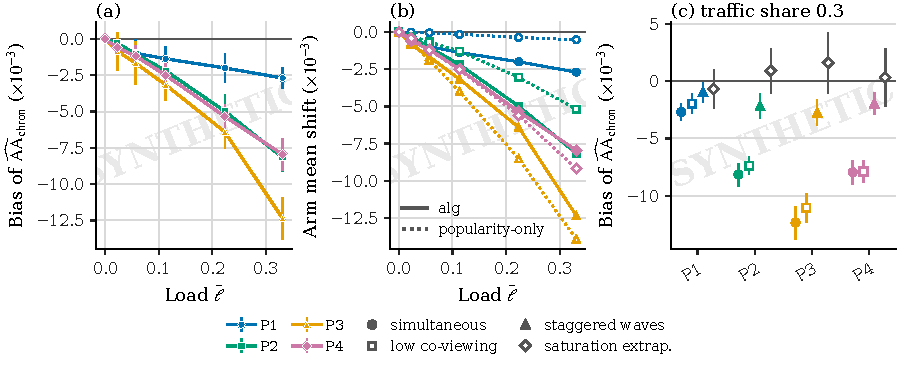
\includegraphics[width=0.94\textwidth]{figures/fig-sim-interference.pdf}
\caption{Synthetic data, E2: interference through shared popularity ($R=24$ paired replications; bars $\pm2$ SE). (a) Bias of the additive amplification relative to the reverse-chronological feed against the load $\bar\ell$, simultaneous design. (b) Shift in mean exposure of the algorithmic arm (solid) and the popularity-only arm (dotted); the reverse-chronological arm does not move. (c) Bias at traffic share $0.3$: simultaneous (load $0.33$), low co-viewing ($0.33$), staggered waves ($0.12$), and randomised-saturation extrapolation from shares $0.1$ and $0.3$.}\label{fig:sim-interference}
\end{figure}

\begin{figure}[tp]
\centering
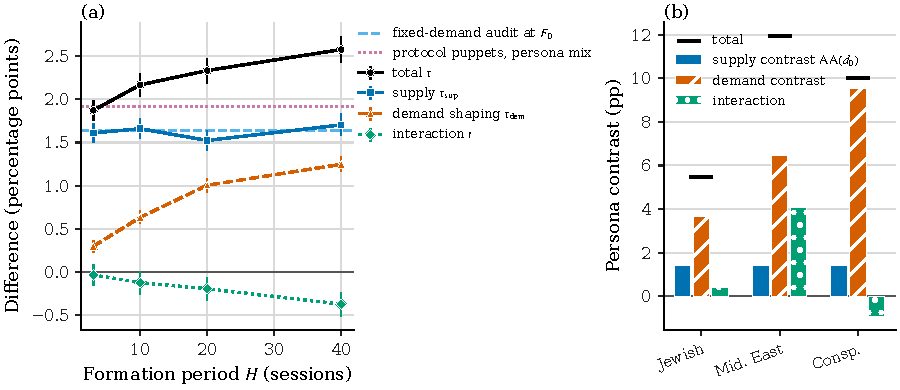
\includegraphics[width=0.94\textwidth]{figures/fig-sim-decomp.pdf}
\caption{Synthetic data, E3: the decomposition of \cref{thm:decomp}. (a) Components for $3{,}000$ synthetic users whose demand evolves, against the length $H$ of the formation period (reference: reverse-chronological; bars $\pm2$ SE over users). Lines: the fixed-demand audit at the initial demand $F_0$, and protocol puppets with the persona mix of the population. (b) Persona-contrast decomposition relative to P1 ($d_0$; protocol puppets, regime ND); black marks: total $\mu_{\mathrm{alg}}(d)-\mu_{\mathrm{ref}}(d_0)$.}\label{fig:sim-decomp}
\end{figure}

\begin{figure}[tp]
\centering
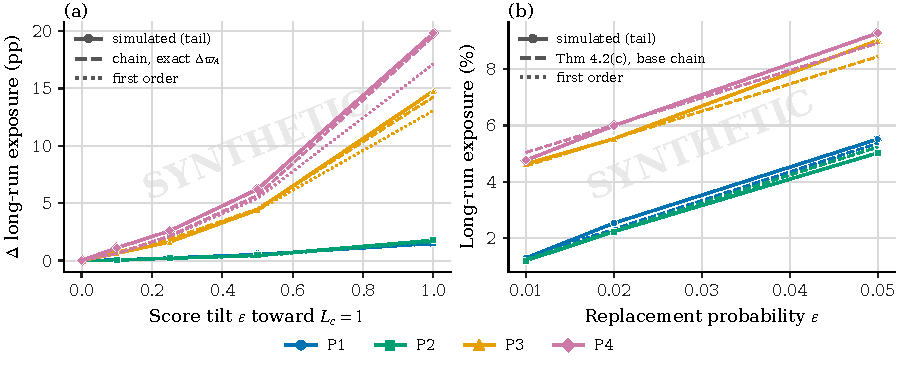
\includegraphics[width=0.94\textwidth]{figures/fig-sim-perturb.pdf}
\caption{Synthetic data, E4: perturbations of the chains of consumed items (algorithmic policy, $250$ naturalistic accounts per persona, common random numbers across $\varepsilon$). (a) Score tilt $\varepsilon$ toward items with $L_c=1$: simulated change in long-run exposure, the exact change between the estimated chains (\cref{thm:perturb}(a)), and its first-order term. (b) Replacement of the next item by an antisemitic one with probability $\varepsilon$: simulation, the closed form of \cref{thm:perturb}(c) from the base chain alone (dashed), and its first-order term $\varpi(\mathcal A)(1+\varepsilon\,\E_\varpi[T_{\mathsf A}])$ (dotted).}\label{fig:sim-perturb}
\end{figure}

\begin{figure}[tp]
\centering
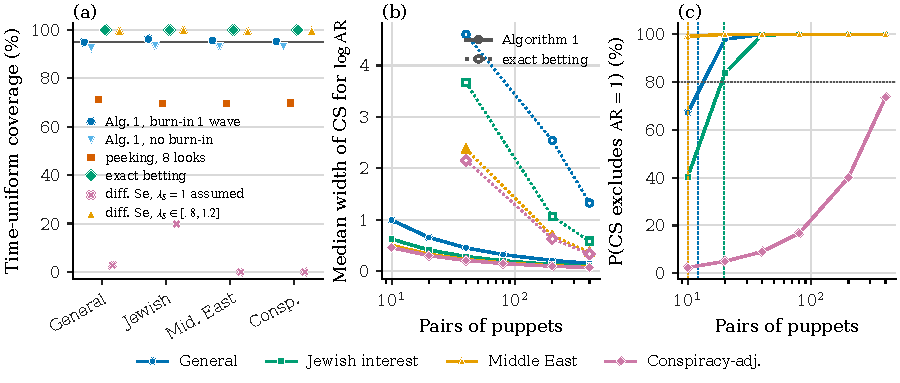
\includegraphics[width=0.94\textwidth]{figures/fig-sim-sequential.pdf}
\caption{Synthetic data, E5 (benchmark: conventional small-lab design, \cref{alg:sequential} on the confirmed-flagged statistic $Y_u$, waves of five pairs, ten sessions per puppet; $R=2{,}000$; exact betting $R=200$). (a) Time-uniform coverage at $\alpha=0.05$ over $80$ waves, with and without one burn-in wave; a fixed-sample interval recomputed after each of the first eight waves (peeking); exact betting; and, under DD, $\lambda_S=1$ assumed or the range $[0.8,1.2]$. (b) Median width for $\log\mathrm{AR}$: \cref{alg:sequential} (solid), exact betting (dotted). (c) Probability of excluding $\mathrm{AR}=1$; dashed verticals: the horizon $n_{\mathrm{seq}}$ of \cref{prop:power}(d), at least two waves (beyond the axis for P4).}\label{fig:sim-sequential}
\end{figure}

\begin{table}[tp]
\centering
\caption{Synthetic data, E1b and E2: checks of \cref{thm:identify,thm:misclass,prop:interference}. E1b: $R=2{,}000$ audits; error rates known unless stated; external validation with $n_1=300$ coded positives and $n_0=1{,}500$ coded negatives. Design effect: $S\sigma^2/\sigma^2_{\mathrm s}$ of \cref{thm:identify} for $S=10$ sessions. Sessions iid: variance that treats the sessions of a puppet as independent. Experiment buckets: every account has a persistent random shift (s.d.\ $1$) in the algorithm's weight on the engagement prior. s.d.\ of $\log\widehat{\mathrm{AR}}$: Monte Carlo, and the median over audits of the delta-method value; $\mathrm{cv}_{\Sp}$ as in \cref{sec:meas-misclass}. Interference block: E2, simultaneous design ($R=24$). There $\xi_\Delta$ is the largest $|\text{bias}|/\bar\ell$ over the grid of loads and $\zeta$ the largest second divided difference of the bias in the load, so the bound of part (a) holds by construction and is attained where the largest ratio occurs.}\label{tab:sim-checks}
\footnotesize
\setlength{\tabcolsep}{3pt}
\simfit{% Generated by code/make_figures.py from results/sim_results.json -- do not edit by hand.
% E1b: R = 2000 audits per configuration; known error rates (thm:identify) unless
% stated; external validation n1 = 300 coded positives, n0 = 1500 coded negatives.
\begin{tabular}{@{}lrrrr@{}}
\toprule
Quantity & General & Jewish interest & Middle East & Conspiracy-adj. \\
\midrule
\multicolumn{5}{@{}l}{\emph{Non-differential error, profiles as simulated (20 puppets per cell)}} \\
Design effect, alg; ref & 1.08; 0.96 & 1.07; 1.01 & 1.23; 1.04 & 1.10; 0.99 \\
Coverage AA: cluster-robust; sessions iid (\%) & 94.2; 94.8 & 94.6; 95.0 & 93.7; 92.8 & 94.2; 94.2 \\
Coverage $\log\mathrm{AR}$: cluster-robust; sessions iid (\%) & 94.5; 95.2 & 95.0; 95.2 & 93.8; 93.2 & 94.1; 94.3 \\
Naive AR; $\omega+(1-\omega)\mathrm{AR}$; true AR & 1.316; 1.325; 1.767 & 1.232; 1.231; 1.334 & 1.532; 1.534; 1.690 & 1.027; 1.033; 1.040 \\
External validation: s.d.\ of $\log\widehat{\mathrm{AR}}$, MC; delta (median) & 0.188; 0.159 & 0.062; 0.061 & 0.050; 0.050 & 0.039; 0.039 \\
\quad $\kappa_{\Sp}=v_{\Sp}^{1/2}/(J\mu_r)$ & 0.246 & 0.081 & 0.053 & 0.039 \\
\quad coverage $\log\mathrm{AR}$; AA (\%) & 94.2; 94.2 & 94.8; 95.3 & 95.0; 94.0 & 94.0; 94.1 \\
\addlinespace
\multicolumn{5}{@{}l}{\emph{Non-differential error, accounts in experiment buckets (20 puppets per cell)}} \\
Design effect, alg; ref & 3.47; 1.04 & 3.61; 1.02 & 5.65; 1.02 & 2.75; 1.03 \\
Coverage AA: cluster-robust; sessions iid (\%) & 93.0; 76.4 & 93.1; 75.6 & 93.0; 62.9 & 93.2; 82.5 \\
Coverage $\log\mathrm{AR}$: cluster-robust; sessions iid (\%) & 94.2; 85.0 & 93.7; 78.5 & 93.3; 69.3 & 93.2; 82.2 \\
\addlinespace
\multicolumn{5}{@{}l}{\emph{Differential error (coded false negatives), external validation, 20 puppets per cell}} \\
True AR; naive $\mathrm{AR}^{\mathrm{nv}}$; $\mathrm{AR}^{\mathrm{pool}}$ (eq.~\ref{eq:mc-diff}) & 1.784; 1.182; 1.494 & 1.353; 1.162; 1.254 & 1.780; 1.349; 1.487 & 1.053; 0.891; 0.861 \\
Corrected, pooled: median AR; coverage (\%) & 1.489; 73.5 & 1.250; 78.5 & 1.483; 15.7 & 0.861; 1.5 \\
Corrected, stratified by arm: median AR; coverage (\%) & 1.765; 97.9 & 1.348; 95.4 & 1.785; 95.0 & 1.050; 95.3 \\
\addlinespace
\multicolumn{5}{@{}l}{\emph{Interference (reference chron): \cref{prop:interference}(a) and (c)}} \\
$|$bias AA$|$; $\xi_\Delta\bar\ell$ at share 0.3 ($\times10^{-3}$) & 2.69; 7.20 & 8.16; 8.16 & 12.35; 12.35 & 7.95; 8.76 \\
$|$bias $\log\mathrm{AR}|$; ratio bound at share 0.3 & 0.088; 0.323 & 0.120; 0.146 & 0.095; 0.110 & 0.070; 0.087 \\
Extrapolation 0.05/0.1: $|$bias$|$; $\zeta\ell_1\ell_2/2$ ($\times10^{-3}$) & 0.61; 0.83 & 0.13; 0.94 & 0.19; 1.44 & 0.10; 1.08 \\
Extrapolation 0.1/0.2: $|$bias$|$; $\zeta\ell_1\ell_2/2$ ($\times10^{-3}$) & 0.73; 3.27 & 0.66; 3.70 & 0.13; 5.67 & 0.37; 4.23 \\
Extrapolation 0.1/0.3: $|$bias$|$; $\zeta\ell_1\ell_2/2$ ($\times10^{-3}$) & 0.69; 4.84 & 0.90; 5.49 & 1.59; 8.41 & 0.31; 6.27 \\
\bottomrule
\end{tabular}
}
\end{table}

\begin{table}[tbp]
\centering
\caption{Synthetic data: summary of E2--E5. E2: bias of the additive amplification relative to the reverse-chronological feed at traffic share $0.3$ ($R=24$; SE $0.4$--$0.7\times10^{-3}$), simultaneous design (load $0.33$), low co-viewing ($0.33$), staggered waves ($0.12$). E3: the ``real users'' are synthetic accounts whose demand evolves. E4: consumed items of naturalistic accounts, and the impression exposure of the same accounts. E4b: slate states of protocol puppets; long-run impression exposure in the second half of a $200$-step session, and its prediction by chains of true, observed and corrected slate states. E5 (benchmark): $R=2{,}000$ audits (MCSE about $0.5$ near $95\%$); coverage over all $80$ waves; peeking: fixed-sample interval after each of waves $1$--$8$; false detection: the sequence excludes $\mathrm{AR}=1$ when it is true; $n_{\mathrm{fix}}$, $n_{\mathrm{seq}}$ from $V_Y$ of \cref{prop:power}(d) for detecting $\mathrm{AR}\ne1$; last row: regime DD.}\label{tab:sim-designs}
\footnotesize
\setlength{\tabcolsep}{3pt}
\simfit{% Generated by code/make_figures.py from results/sim_results.json -- do not edit by hand.
\begin{tabular}{@{}lrrrr@{}}
\toprule
Quantity & General & Jewish interest & Middle East & Conspiracy-adj. \\
\midrule
\multicolumn{5}{@{}l}{\emph{E2: interference (reference chron, traffic share 0.3, load 0.33)}} \\
$\mathrm{AA}^0$ ($\times10^{-3}$) & 14.3 & 18.2 & 54.9 & 3.2 \\
Bias of $\widehat{\mathrm{AA}}$ ($\times10^{-3}$) & $-$2.7 & $-$8.2 & $-$12.3 & $-$8.0 \\
\quad with low co-viewing & $-$2.0 & $-$7.4 & $-$11.1 & $-$7.9 \\
\quad with staggered waves & $-$1.0 & $-$2.2 & $-$2.8 & $-$2.0 \\
\addlinespace
\multicolumn{5}{@{}l}{\emph{E3: real users, formation $H=40$ sessions (pp): $\tau=2.58$, $\tau_{\mathrm{sup}}=1.70$, $\tau_{\mathrm{dem}}=1.25$, $\iota=-0.37$; audit at $F_0$: 1.64}} \\
\addlinespace
\multicolumn{5}{@{}l}{\emph{E4: Markov model, algorithmic policy (consumed items, \%)}} \\
$e_{20}$ predicted / simulated & 0.28 / 0.28 & 0.26 / 0.26 & 3.16 / 3.16 & 3.62 / 3.60 \\
$e_{200}$ predicted / simulated & 0.30 / 0.38 & 0.28 / 0.22 & 3.36 / 3.54 & 3.84 / 3.89 \\
$\kappa_{\mathcal A}$; Kemeny $K$ & 0.50; 2.07 & 0.51; 1.98 & 0.51; 2.04 & 0.52; 2.17 \\
\addlinespace
\multicolumn{5}{@{}l}{\emph{E5: \cref{alg:sequential}, reference chron, waves of 5 pairs, $\alpha=0.05$ unless stated}} \\
True AR & 1.79 & 1.33 & 1.67 & 1.04 \\
Time-uniform coverage, burn-in 1 wave; none (\%) & 95.0; 92.6 & 96.2; 93.5 & 95.7; 93.3 & 95.2; 93.2 \\
\quad peeking, waves 1--8 (\%) & 71.2 & 69.8 & 69.5 & 69.8 \\
Null AR$=1$: false detection by wave 8, Alg.~1; peeking (\%) & 2.9; 30.3 & 2.1; 29.2 & 2.5; 29.8 & 3.4; 33.0 \\
P(excludes AR$=1$) by wave 8 (\%) & 100.0 & 99.8 & 100.0 & 9.0 \\
$n_{\mathrm{fix}}$; $n_{\mathrm{seq}}$ from $A_Y$ (pairs) & 6; 12 & 10; 20 & 2; 4 & 267; 512 \\
Power at $n_{\mathrm{fix}}$ (fixed); by horizon (sequential) & 0.87; 0.92 & 0.85; 0.85 & 0.93; 1.00 & 0.82; -- \\
Differential Se: $\lambda_S$; coverage with $\lambda_S{=}1$; with $[0.8,1.2]$ (\%) & 0.86; 2.8; 99.6 & 0.93; 19.8; 100.0 & 0.83; 0.0; 99.4 & 0.82; 0.0; 99.6 \\
\bottomrule
\end{tabular}
}
\end{table}
}{}
% Supplementary appendix: the full registered protocol summarised in Section 8.
\IfFileExists{appendix/D-protocol.tex}{% =====================================================================
%  Appendix D -- Registered protocol (supplementary). Full text of the protocol
%  summarised in Section 8 (sections/08-protocol.tex); the two are one registration.
%  Owner: TEXT-REVISER (moved from Section 8; labels preserved).
% =====================================================================
\providecommand{\Se}{\mathrm{Se}}
\providecommand{\Sp}{\mathrm{Sp}}
\providecommand{\PPV}{\mathrm{PPV}}
\providecommand{\FOR}{\mathrm{FOR}}

\section{Registered protocol}\label{app:protocol}

This appendix is the full text of the protocol summarised in \cref{sec:protocol}. The stopping and decision rules and the feasibility gate are stated in \cref{sec:prot-stopping,sec:prot-power}, and the ethical and legal conditions in \cref{sec:ethics}. Every number below is a design input, a cap, or an evaluation of a closed form at stated illustrative inputs; none is a result.

\subsection{Service, surface and access route}\label{sec:prot-scope}

The unit of audit is one recommendation \emph{surface} (for example a home feed, or a list of items recommended next to the current one) of one service, in one jurisdiction, during one audit window. The service and surface are chosen at registration by three criteria, in this order:
\begin{enumerate}[(i)]
  \item \emph{A reference policy is available.} AR and AA require exposure under a reference policy $\pi=\mathrm{ref}$ (\cref{def:amplification}). On a live service, the candidates are the non-profiling option that very large online platforms must offer under Article~38 of the DSA, or a reverse-chronological option where offered (\cref{sec:bg-governance}), and logged-out sessions (\cref{sec:bg-debates}). The random-from-eligible-pool and popularity-only reference policies of \cref{def:amplification} are not generally available to an outside auditor. They are evaluated in \cref{sec:simulation}, and on a live service only if data obtained under Article~40(4) permit it. If no reference policy is available for a surface, no amplification is estimated for it.
  \item \emph{A lawful access route exists.} In order of preference: data obtained as a vetted researcher under Article~40(4) of the DSA, or through a research interface the provider offers, where these can deliver exposure under a fixed demand profile; access to publicly accessible data under Article~40(12); and a sock-puppet audit only where neither route can identify the estimand, and only after the legal review and ethics approval of \cref{sec:ethics}.
  \item \emph{The classifier is validated for the content.} The service's dominant language(s) and formats (text, images, video transcripts) must be covered by the frozen classifier and by the annotators of \cref{sec:prot-validation}.
\end{enumerate}
The jurisdiction is an EU Member State, so that the DSA routes apply and the Article~38 option is in scope. All puppets present from that jurisdiction.

\subsection{Personas, puppets and sessions}\label{sec:prot-personas}

\paragraph{Personas}
A persona $d$ is a demand profile. It has three components: a pool of seed items used to train the account; a choice rule that selects one item from each slate; and an interaction budget. There are four candidate personas, listed in the registered order of priority that the feasibility gate of \cref{sec:prot-power} uses. The gate selects the set $\mathcal D_A$ of confirmatory personas from them. Their seed pools are compiled and screened before registration, and two coders confirm that no seed item is antisemitic under the codebook of \cref{sec:prot-validation}.
\begin{enumerate}[(a)]
  \item \emph{Jewish interest}: Jewish culture, religion, history and community news. Users who seek such content may be targeted by antisemitic replies and recommendations, so this persona measures what the algorithm supplies to an audience that is often the target of the content.
  \item \emph{Conspiracy-adjacent}: content on conspiracy theories about elites, finance or health that is not itself antisemitic under the codebook. This is the persona whose demand lies closest to antisemitic content without requiring any engagement with it.
  \item \emph{Middle East news}: news and commentary on Israel, the Palestinian territories and the region, drawn from a seed pool balanced across outlets and viewpoints by two coders working independently.
  \item \emph{General interest} ($d_0$, the baseline): mainstream news, sport, entertainment and how-to content.
\end{enumerate}
The first two come first because they ask the questions that motivate the audit. The baseline persona is needed mainly for the persona-contrast decomposition (\cref{sec:prot-estimands}), which is estimated only if all four personas are audited. No persona is trained on antisemitic content. A persona that sought it out would inflate the engagement metrics of hateful items, which the protocol forbids (\cref{sec:eth-footprint}). The audit therefore asks what each policy \emph{supplies} to profiles whose demand is legitimate or adjacent, not what it delivers to users who seek antisemitic content.

\paragraph{Choice rule and the avoid-on-flag constraint}
At each step $t$ the puppet observes a slate. The first $k$ positions are recorded and scored by the frozen classifier. The puppet then opens the highest-ranked recorded item whose score is below a registered threshold $s_{\mathrm{safe}}$ and whose similarity to the persona's seed pool exceeds a registered threshold. If no recorded item meets both conditions, it opens the highest-ranked recorded item below $s_{\mathrm{safe}}$. If there is none, it opens the first item below $s_{\mathrm{safe}}$ further down the slate, which is recorded but not counted among the exposure positions. Items scoring above $s_{\mathrm{safe}}$ are recorded as exposures but never opened. The threshold $s_{\mathrm{safe}}$ lies below the classifier's decision threshold, so that no flagged item is opened. It is set conservatively enough that the pilot's estimate of the share of openings that are false negatives is small (\cref{sec:prot-interference}). The choice rule is part of the persona, so it is applied identically under both policies, and $\mathrm{AR}(d)$ is defined conditional on it (\cref{asm:id-script}). Because the rule depends on the classifier, false negatives can still be opened. Their share is estimated from coded openings (\cref{sec:prot-validation}), and it enters the interference analysis (\cref{sec:prot-interference}) and the residual footprint (\cref{sec:eth-footprint}).

\paragraph{Exposure}
Exposure counts \emph{impressions}, which settles the choice that \cref{sec:est-setup} leaves to the protocol. The exposure $E_{us}$ of session $s$ of puppet $u$ is the share of its $kT$ recorded positions, $k$ at each of $T$ steps, that show an item with $L_c=1$, and the flagged share $Q_{us}$ is the share with $\widehat L_c=1$, exactly as in \cref{sec:id-design}. An item recorded at several positions counts at each, and opening an item adds no further impression. Exposure is therefore not a property of the items a puppet opens. Under the avoid-on-flag rule, an opened item is antisemitic only if it is a false negative. The registered $k$ is the number of items visible without scrolling on the surface's default layout, fixed during the pilot. With $k=1$, exposure reduces to the top-ranked item. \Cref{sec:prot-estimands} describes how the Markov model of \cref{sec:markov} is fed with these impressions.

\paragraph{Session structure and waves}
Each puppet passes through a \emph{training phase} of $S_{\mathrm{train}}$ sessions, one per day, in which it opens a random subset of its persona's seed pool with a fixed dwell time per item. A \emph{measurement phase} of $S$ sessions follows, at most one per day at a randomised time, each of $T$ steps from a registered entry point (the home surface, or a seed item drawn at random from the pool). Drawing a different random subset of seeds for each puppet limits the overlap in viewing between puppets of the same persona, which is a channel of interference (\cref{sec:prot-interference}). Puppets run in waves. A wave occupies $S_{\mathrm{train}}+S$ days, and consecutive waves are separated by a washout in which no audit account is active (\cref{sec:prot-interference}). With the candidate values of \cref{tab:prot-design}, a wave cycle lasts three weeks. \Cref{tab:prot-design} lists the design parameters and how each is fixed.

\begin{table}[htbp]
\centering
\caption{Design parameters of the audit. Candidate values are illustrative and are fixed at registration, by the pilot or by the feasibility gate, as indicated; none is a result.}\label{tab:prot-design}
\footnotesize
\setlength{\tabcolsep}{4pt}
\renewcommand{\arraystretch}{1.15}
\begin{tabularx}{\textwidth}{@{}>{\raggedright\arraybackslash}p{4.5cm}>{\raggedright\arraybackslash}p{4.0cm}>{\raggedright\arraybackslash}X@{}}
\toprule
Parameter & Candidate & Fixed by \\
\midrule
Confirmatory personas $\mathcal D_A$ & 1, 2 or 4 of the 4 candidates, in priority order & Feasibility gate (\cref{sec:prot-power}) \\
Policy arms & alg, ref & Reference policy available on the surface (\cref{sec:prot-scope}) \\
Pairs per persona $n$ (trained puppets per arm) & From the gate; $122$ on rung R4 under the inputs of \cref{tab:prot-power} & \Cref{prop:power} with pilot inputs (\cref{sec:prot-power}) \\
Capacity caps: accounts $U_{\max}$ (all accounts created, pilot and sentinels included); coded positions (pilot included) & 400; 15{,}000 & Registration, with ethics approval and budget (\cref{sec:eth-footprint,sec:eth-annotators}) \\
Wave budget $W_{\max}$; washout between waves & 6; at least 14 days & Registration; washout checked in the pilot (\cref{sec:prot-interference}) \\
Load cap $\ell_{\max}$ & 0.01 & Registration (\cref{sec:prot-interference}) \\
Burn-in $b$; tuning constant; planned pairs & 1 wave; $a=-2\log\alpha+\log(1-2\log\alpha)$; $n^\ast=n$ & Registration (\cref{alg:sequential}) \\
Training sessions $S_{\mathrm{train}}$; seeds opened per session & 3; 10 & Pilot (stability of recommendations) \\
Measurement sessions $S$ per puppet & 4 & \Cref{prop:power}(b) with pilot costs and variances \\
Steps per session $T$; positions recorded $k$ & 20; visible slate ($5$ in \cref{tab:prot-power}) & Pilot; surface layout \\
Codes per puppet: flagged $m$; unflagged $m'$ & 10; 25 (5 of them openings) & \Cref{alg:sequential}; pilot (\cref{sec:prot-validation}) \\
Sentinel puppets per arm and wave (not coded) & 2 & Fixed \\
Pilot: trained puppets per cell; coding & 10; all flagged and 50 unflagged positions per puppet & Fixed (\cref{sec:prot-power}) \\
Error level $\alpha$; margin $\delta$; power & 0.05; 1.25; 0.8 at $\mathrm{AR}=\delta^2$ & Registration (\cref{sec:prot-stopping}) \\
Range $[\lambda_-,\lambda_+]$ for $\lambda_S$ (secondary analysis) & $[0.95,1.05]$ & Registration (\cref{sec:prot-estimands}) \\
\bottomrule
\end{tabularx}
\end{table}

\subsection{Randomisation}\label{sec:prot-randomisation}

All accounts are created in the same way, before any is assigned, so that features of account creation cannot differ systematically by arm. The audit runs in waves $w=1,\dots,W$, with $W\le W_{\max}$, that are separated by washouts. Within each wave, puppets are assigned completely at random to the persona--policy cells of the confirmatory personas, in equal numbers per arm. Persona training is therefore randomised, and policy is randomised independently of it. Seed subsets, session start times and the order in which puppets run within a day are also randomised. All puppets are trained in the same way whatever their arm. The policy contrast is applied only at the start of the measurement phase: puppets in the reference arm switch to the non-profiling or chronological option, or run their measurement sessions logged out with the same choice rule. Training is thus identical in distribution across arms, and the only systematic difference at measurement is the policy. This is the design of \cref{thm:identify}.

Waves are blocks. Every wave contains both arms of every confirmatory persona, so a change in the service's policy during the window affects both arms of a wave equally. The pairs of \cref{alg:sequential} are formed within waves, by pairing each puppet of the algorithmic arm at random with a distinct puppet of the reference arm of the same wave and persona. The wave weights $\omega_w$ of the blocked estimator of \cref{thm:identify}(d) are the shares of pairs, so that the blocked estimator and the confidence sequence target the same window average (\cref{sec:prot-monitoring}). If attrition leaves the arms of a wave unequal, the surplus puppets are excluded from the pairs at random, and attrition is reported by arm. On rungs R1 and R2, if at least four waves are run, wave sizes are randomised for the saturation design of \cref{sec:prot-interference}: consecutive waves are grouped in pairs, and one wave of each pair, chosen at random, has twice as many puppets per cell as the other. On rungs R3 and R4 all waves have equal size (\cref{sec:prot-power}). Changes announced by the service during the window are logged as they occur.

\subsection{Interference controls}\label{sec:prot-interference}

Puppets share the learning system they audit. Through it, one puppet's behaviour can change what another is shown, which violates \cref{asm:id-nointerf}. The protocol limits interference by design, keeps the load within a registered cap, and collects evidence about what remains, so that the bound and the breakdown value of \cref{prop:interference} can be reported. It cannot estimate the constants $\xi_\pi$ and $\xi_\Delta$ of \cref{asm:id-bounded}, because no audit observes the no-audit state $\ell=0$.
\begin{itemize}
  \item \emph{Isolation.} Puppets never follow, message, mention or otherwise interact with any account, including each other. Each runs in its own browser profile with separate storage, and no identifier is shared between puppets.
  \item \emph{Limited co-viewing in training.} Each seed item may be opened by at most a registered number of puppets per wave, and seed subsets are drawn so that puppets of the same persona overlap as little as the pool allows.
  \item \emph{Washout.} Consecutive waves are separated by at least $14$ days in which no audit account, sentinels included, is active, so that waves are the non-interfering groups of \cref{asm:id-bounded}. The length is fixed at registration from what the service publishes about its update cycles, and it is checked in the pilot, whose sentinels run before, during and after the wave. The washout is lengthened if their exposure has not returned to its pre-wave level. No washout resets engagement counters that the service accumulates without decay, so the load is computed cumulatively: the openings of earlier waves count against the items' cumulative engagement.
  \item \emph{Load cap.} After each wave, an approximate upper bound on its load $\ell_w$ is computed from public engagement counts, as the puppets' openings of the items they opened divided by the increase in those items' public engagement counts, cumulated as above. The registered cap is $\ell_{\max}=0.01$. Wave sizes are set at the gate so that the load projected from the pilot stays below the cap. If a confirmatory wave exceeds it, later waves are made smaller and the deviation is reported. Within a wave, staggered start times lower the instantaneous load further.
  \item \emph{Device and network hygiene.} Each puppet keeps one consistent device profile and one stable network location within the study jurisdiction for its whole life. Network locations are not rotated to evade a service's detection or rate limits, and no technical access control is circumvented (\cref{sec:eth-legal}). A puppet that is challenged, restricted or suspended is stopped and not replaced within the wave. Its attrition and the reason are recorded, and attrition is compared across arms.
  \item \emph{False-negative mass.} Because false negatives are opened, some audit engagement reaches antisemitic items. By \cref{prop:interference}(b), whether load then raises or lowers exposure depends on how concentrated this engagement is on antisemitic items, relative to the baseline exposure. We estimate the share of openings that are false negatives, $\chi_{\mathrm{open}}$, an unweighted analogue of $\chi^{\mathrm P}$ in \cref{prop:interference}(b), from the coded openings (\cref{sec:prot-validation}). We report it with its confidence interval next to the estimated exposures $\mu_\pi(d)$. We make no claim about the sign of the interference bias, and we use only the two-sided bound of \cref{prop:interference}(a) and the breakdown value of part (d). If the pilot's upper Clopper--Pearson bound for $\chi_{\mathrm{open}}$ is not small relative to the pilot exposures, $s_{\mathrm{safe}}$ is lowered before the first confirmatory wave.
  \item \emph{Sentinels.} In each wave, two untrained puppets per arm run measurement sessions alongside the trained puppets. Across waves of different load, the slope of their exposure in the load is evidence about interference for an untrained profile. It is neither an estimate of $\xi_\Delta$ for the audited personas, whose sensitivity to load can differ, nor a bound on it. Sentinels also track drift that is common to both arms.
  \item \emph{Randomised saturation.} When wave sizes are randomised, on rungs R1 and R2 (\cref{sec:prot-randomisation}), the two load levels satisfy $\ell_2\approx2\ell_1\le\ell_{\max}$. \Cref{prop:interference}(c) then gives a test of differential interference and the extrapolated estimator $\widehat{\mathrm{AA}}^{\mathrm{ex}}$. Its variance is several times that of the blocked estimator, so it is a robustness analysis, and even on rungs R1 and R2 the test has little power. Under \cref{asm:id-bounded}, $|\mathrm{AA}(\ell_2)-\mathrm{AA}(\ell_1)|\le\xi_\Delta(\ell_1+\ell_2)$ by the triangle inequality, so the saturation contrast also gives a data-based lower value for the interference constant, $|\widehat{\mathrm{AA}}(\ell_2)-\widehat{\mathrm{AA}}(\ell_1)|/(\ell_1+\ell_2)$.
\end{itemize}

\paragraph{Reporting}
For each confirmatory persona we report the bound on $\bar\ell$, the estimate of $\chi_{\mathrm{open}}$, the sentinel slopes, the saturation slope where available, and the breakdown value $\xi^\ast$ of \cref{prop:interference}(d). Because the final analysis follows sequential monitoring, $\xi^\ast$ is computed with the radius of the confidence sequence for $\mathrm{AA}(d)$ (\cref{sec:prot-monitoring}) in place of $z_{1-\alpha/2}\widehat{\mathrm{se}}$. The product $\xi^\ast\bar\ell$ is the largest shift of $\mathrm{AA}(d)$ by differential interference that leaves the sign of the conclusion intact, and it is stated with every conclusion. A conclusion whose $\xi^\ast$ lies below the lower value from the saturation contrast is reported as \emph{fragile to interference}.

\subsection{Classifier and validation sample}\label{sec:prot-validation}

\paragraph{Frozen classifier}
The classifier follows the lab's detection proposal \citep{kornsteinlab2026detection}. Its version, decision threshold, $s_{\mathrm{safe}}$ and the score band that defines the observed borderline state of the Markov analysis are fixed and hashed at registration and are not changed during the audit. Every recorded item receives a score; $\widehat L_c$ is the thresholded score.

\paragraph{What the validation must deliver}
Three requirements of \cref{sec:identification,sec:measurement} fix the design. First, error rates must be estimated by arm, because they differ when the arms show different content (\cref{thm:misclass}(c)), and by persona, because persona contrasts need the error rates of each persona (\cref{thm:identify}(a)). Second, they must be exposure-weighted, as in \eqref{eq:id-sesp}, because the target is the classifier's performance on what each cell is shown, not on distinct items. Third, coding must be done within puppets. \Cref{alg:sequential} codes each puppet's flagged positions, and puppet-level double sampling makes each puppet's corrected exposure conditionally unbiased (\cref{thm:misclass}(d)), so that the cluster-robust variance carries the validation uncertainty. The validation floors of \cref{prop:power}(a) decide between the designs that meet these requirements. Under the inputs of \cref{tab:prot-power}, a Rogan--Gladen correction with error rates estimated by arm from coded negatives needs about $21{,}400$ coded negatives per arm and persona on rung R1 before any number of puppets suffices. Internal double sampling needs about $2{,}600$ coded unflagged exposures per arm and persona, and its coding grows with the number of puppets. A fixed validation sample of $2{,}000$ items, as in a conventional small-lab design, would give about $125$ per arm and persona. The protocol registers double sampling within puppets.

\paragraph{Sampling within puppets}
For each puppet, after its last measurement session, recorded positions are drawn from its own record for coding, in three strata:
\begin{enumerate}[(i)]
  \item $m=10$ flagged positions, uniformly without replacement, or all of them if the puppet has fewer, as \cref{alg:sequential} requires;
  \item $5$ positions of items that the puppet opened, which estimate the false-negative share of openings $\chi_{\mathrm{open}}$;
  \item $20$ other unflagged positions, stratified by registered classifier-score bands, with the allocation across bands set by the rule of \citet{neyman1934} from pilot estimates of the false-omission rate in each band.
\end{enumerate}
Strata (ii) and (iii) make up the $m'=25$ unflagged codes per puppet. Within a stratum, every recorded position has the same probability of being drawn, so an item shown at several positions is proportionally more likely to be drawn, and each drawn position is weighted by its stratum's size divided by the number drawn from it. The sample therefore represents exposures, not distinct items. A distinct item drawn more than once, within a puppet or across puppets, is coded once, and its adjudicated label is attached to every draw. Coding effort is thus counted in distinct items, while estimation is per exposure. In the pilot, all flagged positions and $50$ unflagged positions per puppet are coded, to estimate the inputs of \cref{sec:prot-power} and the false-omission rate by score band.

\paragraph{Coding}
Two trained annotators code each sampled item independently. They are blind to arm, persona, puppet, stratum and classifier score; items from all strata and cells are interleaved in mixed batches, and they work from a written codebook. The codebook has four primary categories: \emph{antisemitic} (including coded forms); \emph{quotes, reports or criticises antisemitism}; \emph{borderline or ambiguous}; and \emph{not antisemitic}. It also has a flag for content concerning Israel or Zionism. The primary label is $L_c=1$ for the first category only. Sensitivity analyses count borderline items as antisemitic, and report scope variants under the IHRA and JDA definitions where they differ \citep{ihra2016,jda2021}, side by side and without a preferred variant. A third, senior coder adjudicates disagreements; items are not dropped. Annotators complete a calibration round on items outside the audit until their agreement reaches a registered threshold. Agreement is reported as Cohen's kappa \citep{cohen1960}, overall and by stratum. Coders must be fluent in the languages of the items. The protections for annotators are those of \cref{sec:eth-annotators}.

\paragraph{Use}
For each puppet, the adjudicated labels give the \emph{double-sampled exposure} $\widetilde E_u$: the right side of \eqref{eq:mc-ds} computed from the puppet's own codes, with the unflagged stratum split into the strata above, each weighted by its share of the puppet's recorded positions. Each coded unflagged position thus stands for about $16$ recorded positions. Given the puppet's record, $\widetilde E_u$ is unbiased for its true exposure $\bar E_u$ (\cref{thm:misclass}(d)), and it lies in $[0,1]$. It assumes nothing about sensitivity or specificity, in either arm or in any persona, and it is the primary outcome. Aggregated over the puppets of a cell, the same codes give exposure-weighted estimates of $\Se_\pi(d)$, $\Sp_\pi(d)$, $\PPV_\pi(d)$ and $\FOR_\pi(d)$, and of the sensitivity ratio $\lambda_S(d)$. We report them by cell, with tests of equal error rates across arms within each persona and across personas, and we report naive, pooled Rogan--Gladen and double-sampled estimates side by side. For the pooled correction we also report $\mathrm{cv}_{\Sp}$ and a bootstrap over puppets and codes (\cref{sec:meas-misclass}). False negatives are rare among unflagged exposures, so under the inputs of \cref{tab:prot-power}, and before any gain from score bands, the double sample pins $\lambda_S(d)$ down only to within a factor of about $1.13$ at $95\%$ confidence on rung R4, and about $1.06$ even on rung R1. The range registered for $\lambda_S$ in the secondary analysis (\cref{sec:prot-estimands}) is therefore an assumption that the audit can contradict but not confirm.

\subsection{Estimands and analysis}\label{sec:prot-estimands}

\paragraph{Primary}
For each confirmatory persona $d\in\mathcal D_A$, the amplification ratio $\mathrm{AR}(d)$ and the additive amplification $\mathrm{AA}(d)$ of \cref{def:amplification}, comparing the algorithmic policy with the registered reference policy, with exposure measured in impressions (\cref{sec:prot-personas}). They are estimated from the double-sampled exposures $\widetilde E_u$, blocked by wave as in \cref{thm:identify}(d), with wave weights equal to the shares of pairs. Under drift, the estimands are the window-averaged $\overline{\mathrm{AR}}(d)$ and $\overline{\mathrm{AA}}(d)$ of \cref{thm:identify}(d) for the waves actually run, and every conclusion is indexed by the window (\cref{sec:id-drift}). Inference is by the confidence sequences of \cref{sec:prot-monitoring}. No population weighting $\Lambda$ of personas is registered, so no population-weighted estimand is reported (\cref{sec:est-amp}). If the pilot's upper Clopper--Pearson bound for $\mu_{\mathrm{ref}}(d)$ lies below the registered floor ($0.002$ illustratively), the ratio is unstable for that persona, and $\mathrm{AA}(d)$ becomes its primary estimand, with the stopping rules of \cref{sec:prot-stopping} applied to the sequence for $\mathrm{AA}(d)$ and the registered additive margin $\delta_{\mathrm A}$ ($0.005$ illustratively) in place of $\log\delta$.

\paragraph{Secondary}
\begin{enumerate}[(i)]
  \item \emph{Confirmed-flagged analysis.} \Cref{alg:sequential} as stated, on the confirmed-flagged exposures $Y_u$, with the registered range $[\lambda_-,\lambda_+]=[0.95,1.05]$ for $\lambda_S(d)$. We also report the largest symmetric range $[1/\lambda^\dagger,\lambda^\dagger]$ for which its conclusion would still hold. This analysis uses no unflagged codes but assumes the range. The primary analysis assumes nothing about $\lambda_S$ and pays for it with the unflagged codes.
  \item \emph{Persona-contrast decomposition}, only if all four personas are audited (rung R1 of \cref{sec:prot-power}). For each persona $d$ relative to the baseline $d_0$, we report the supply contrast $\mathrm{AA}(d_0)$, the demand contrast $\mu_{\mathrm{ref}}(d)-\mu_{\mathrm{ref}}(d_0)$ and the interaction $\mathrm{AA}(d)-\mathrm{AA}(d_0)$, with their Shapley shares (\cref{sec:est-audit}). The cell means are those of $\widetilde E_u$, so each is corrected with its own persona's and arm's error rates, as contrasts across personas require (\cref{thm:identify}(a)). The demand contrast compares two scripted personas. It is not the demand-shaping effect $\tau_{\mathrm{dem}}$ of \cref{thm:decomp}, which no fixed-demand audit identifies (\cref{prop:audit-scope}).
  \item \emph{Markov exposure summaries}, fed as described below and reported as exploratory, model-based analyses.
% ALIGN-WITH-SIM: exploratory status, aligned with E4b (07, sec:sim-markov).

  \item \emph{Diagnostics}: the interference reporting of \cref{sec:prot-interference}; the drift statistic $X^2_{\mathrm{drift}}$ of \cref{sec:id-drift}, the wave-level estimates and the sentinel series; attrition by arm; error rates by cell and their equality across arms and personas; and the exact betting sequence of \cref{thm:sequential}(b) at the stopping time.
\end{enumerate}

\paragraph{Feeding the Markov model}
\Cref{sec:markov} models a session as a chain of items, one per step. The protocol measures exposure on slates of $k$ recorded positions. Under the avoid-on-flag rule, the chain of \emph{opened} items visits $\mathcal A$ only through false negatives, so its exposure functionals would describe the residual footprint, not exposure. We therefore apply \cref{sec:markov} with the slate of step $t$ in the role of the item. The state $X_t\in\{\mathsf N,\mathsf B,\mathsf A\}$ is the most severe true state among the $k$ recorded positions of step $t$: $\mathsf A$ if any of them is antisemitic, $\mathsf B$ if none is but one is borderline, and $\mathsf N$ otherwise. Then $\ind{X_t\in\mathcal A}$ records whether the slate of step $t$ shows antisemitic content, and $e_T(P,\nu)$ of \eqref{eq:mk-eT} is the expected share of steps whose slate does. The matrix $P_\pi(d)$ describes transitions between consecutive slates, so it combines what the policy offers with what the persona opened. Let $\bar k_{\mathcal A}$ be the mean number of antisemitic positions in a slate in state $\mathsf A$. If $\bar k_{\mathcal A}$ does not depend on the step, which we check by comparing early and late steps, the impression exposure of the primary analysis is $\mu_\pi(d)=e_T\{P_\pi(d),\nu_\pi(d)\}\,\bar k_{\mathcal A}/k$, and its long-run analogue is $\varpi(\mathcal A)\,\bar k_{\mathcal A}/k$. A ratio of chain functionals between the arms must then be multiplied by the ratio of the arms' $\bar k_{\mathcal A}$, which is reported. If the order tests of \citet{anderson1957} reject a first-order chain on pilot data, the state is enlarged to the pair formed by the slate state and the state of the item opened at the previous step, as \cref{sec:markov-model} allows. The slate states are observed through the classifier, with the borderline state defined by the registered score band. The observed transition counts are corrected as in \cref{sec:markov-estimation}, with a slate-level confusion matrix $\Gamma$ computed from each cell's item-level error rates under the independence of errors across positions assumed there. A neutral slate is misread as $\mathsf A$ with probability about $k(1-\Sp)$, so the correction is large.
% ALIGN-WITH-SIM: E4b result on slate-state chains, aligned (07, sec:sim-markov).
The correction is applied to the two states $\{\mathsf A,\text{not }\mathsf A\}$; the three-state chain is reported only if the pilot shows that the borderline score band separates $\mathsf B$ from $\mathsf N$, because otherwise the slate confusion matrix is nearly singular. In simulation, the uncorrected slate chain erred by up to $150\%$ and could reverse the comparison of the arms, while the corrected two-state chain erred by at most $7\%$ in the long run, with a standard deviation of the log ratio of the arms up to $2.3$ times that of the session average (\cref{sec:sim-markov}).
The variance of every chain functional is obtained by a bootstrap over puppets, because the sessions of one puppet are correlated. The stationary exposure, the hitting times of $\mathsf A$ and the sensitivities of \cref{prop:markov,thm:perturb} are model-based and are reported as such. At the audited horizon, the session averages of the primary analysis take precedence, as \cref{sec:markov-estimation} recommends. The opened-item chain is reported descriptively.

\paragraph{Exploratory}
Exposure by slate position, and heterogeneity by entry point.

\subsection{Sequential monitoring}\label{sec:prot-monitoring}

\paragraph{The primary sequences}
After each wave, \cref{alg:sequential} is run for every confirmatory persona with the outcome $O_u=\widetilde E_u$ and the range $\{1\}$ for $\lambda$, because the ratio of the arms' mean double-sampled exposures is $\mathrm{AR}(d)$ itself (\cref{thm:misclass}(d)). The level is $\alpha/|\mathcal D_A|$ per persona, so that the family of sequences has simultaneous coverage $1-\alpha$ to the same approximation. The registered burn-in is $b=1$ wave: the first confirmatory wave updates the estimates but can neither narrow the running interval nor stop the audit. The tuning constant is $a=-2\log\alpha+\log(1-2\log\alpha)$ at the per-persona level, and the planned horizon $n^\ast$ is the $n$ fixed at the gate. The same construction applied to the pair differences $\widetilde E_{a,i}-\widetilde E_{r,i}$ gives a confidence sequence for $\mathrm{AA}(d)$. It needs no delta method, because the differences are independent and identically distributed with mean $\mathrm{AA}(d)$, so \cref{lem:seq-crossing} applies with $R_n=0$.

\paragraph{What the guarantee is}
The coverage of these sequences is approximate, not exact. \Cref{thm:sequential}(a) is a large-sample statement, in which the planned horizon and the burn-in grow together, and it assumes no interference (\cref{asm:id-nointerf}), stable policies (\cref{asm:id-stable}(a)) and scripted demand (\cref{asm:id-script}). At the protocol's sizes, the probability that monitoring after every wave and stopping early produces a wrong conclusion is therefore close to its nominal level but is not guaranteed to stay below it. Simulation shows that it can exceed the nominal level when there are few pairs per wave (\cref{sec:meas-sequential}), and the double-sampled outcome is heavy-tailed, because each coded unflagged position stands for about $16$ recorded positions.
% ALIGN-WITH-SIM: E5b result on coverage and the pilot check, aligned (07, sec:sim-sequential).
In the simulation of the registered design (waves of $20$ pairs, $W_{\max}=6$, $b=1$), $\widetilde E_u$ had excess kurtosis of up to about $13$ in the arms and up to $47$ in a null case, yet the sequences for $\mathrm{AR}$ and $\mathrm{AA}$ covered in $98.4$--$99.4\%$ of audits at $\alpha=0.05$ and $99.1$--$99.8\%$ at $\alpha=0.025$, and the betting fallback, though valid, was nearly powerless at $120$ pairs (\cref{sec:sim-sequential}).
The resampling check of \cref{sec:prot-stopping} draws pairs with replacement from the ten pilot puppets per cell, so it reproduces only the tails that the pilot happens to contain. It can reveal a gross failure of the approximation; it cannot certify coverage. If it fails, the exact betting sequence becomes the primary sequence, and its horizon is found by the same resampling.

\paragraph{Drift}
Under drift, the pairs are independent but not identically distributed. The sequences then target the ratio of window-averaged means (\cref{sec:meas-sequential}), here $\overline{\mathrm{AR}}(d)$ with wave weights equal to the shares of pairs, which is also the target of the blocked estimator, and the guarantee holds only approximately. Blocking by pairing within waves keeps drift from being mistaken for amplification, but it does not remove drift from the estimand (\cref{sec:id-drift}). We report the wave-level estimates and $X^2_{\mathrm{drift}}$ with every conclusion. If the service announces a change to the audited surface during the window, the waves before and after it are reported separately as well as together. No conclusion is extended beyond the window.

\paragraph{Robustness}
The registered robustness checks are: naive, pooled Rogan--Gladen and double-sampled estimates; the confirmed-flagged analysis and its $\lambda^\dagger$; the exact betting sequence; scope variants of the label; analyses by wave block; the exclusion of puppets with attrition; the saturation-extrapolated estimator; and the sensitivity of each conclusion to interference through $\xi^\ast$.

\subsection{How the sample sizes are computed}\label{sec:prot-sizes}

\paragraph{Illustrative inputs}
\Cref{tab:prot-power} evaluates the closed forms of \cref{prop:power} for the design of this protocol. The inputs are illustrative assumptions, and the pilot replaces them. Reference exposure is $\mu_{\mathrm{ref}}(d)=0.02$ for every persona. The session-level coefficient of variation of true exposure is $1$, and the intra-puppet correlation is $\gamma=0.3$. A puppet runs $S=4$ measurement sessions of $kT=100$ recorded positions ($k=5$, $T=20$). The classifier has $\Se=0.85$ and $\Sp=0.98$ in both arms. Power is $0.8$ at the registered alternative $\mathrm{AR}=\delta^2$, with $\delta=1.25$. Each puppet has $m=10$ flagged and $m'=25$ unflagged codes, and the cost ratio is $c_p/c_s=3$, a puppet's training costing about three sessions. The candidate $S=4$ rounds up $S^\ast=3.6$ of \cref{prop:power}(b). It needs more puppets than $S=10$ (the row ``R1, $S=10$ sessions'' of \cref{tab:prot-power}), but fewer sessions in all, and sessions are the audit's footprint. For the double-sampled statistic, the coding variance of a puppet does not fall with $S$, which lowers $S^\ast$, while the coding cost of a puppet raises it. The pilot fixes $S$ by the minimisation of \cref{prop:power}(b) with both included.

\paragraph{How the sizes are computed}
For the primary analysis, the double-sampled outcome has variance $V^{\mathrm{ds}}+nV_{\mathrm{val}}^{\mathrm{ds}}$ per pair, with $V^{\mathrm{ds}}$ as in \cref{prop:power}(a) and $V_{\mathrm{val}}^{\mathrm{ds}}$ of \eqref{eq:pw-B} evaluated at $m_{1\pi}=nm$ and $m_{0\pi}=nm'$, so that $nV_{\mathrm{val}}^{\mathrm{ds}}$ does not depend on $n$. The horizon is that of \cref{prop:power}(c) with this variance, $n=(c_\alpha+z_{1-\beta})^2(V^{\mathrm{ds}}+nV_{\mathrm{val}}^{\mathrm{ds}})/\Delta^2$. Materiality rungs use $r_0=\delta$ and detection rungs $r_0=1$, both with $r_1=\delta^2$. The other columns of \cref{tab:prot-power} are the fixed-sample size with known error rates (\cref{prop:power}(a) with $V_{\mathrm{val}}=0$), the validation floors $n_0^{\min}$, $n^{\min}_{0,\mathrm{st}}$ and $m_0^{\min}$ of \cref{prop:power}(a), and the horizons of the confirmed-flagged analysis with $\lambda_S=1$ and with the registered range for $\lambda_S$ (\cref{prop:power}(d)).

\paragraph{Feasibility in detail}
Rung R1, materiality for four personas, needs about $4{,}900$ trained accounts and $170{,}000$ coded exposures, and stays in the thousands of accounts in every sensitivity row; rung R2 needs about $2{,}200$ accounts. Detection is much cheaper: rung R3 needs about $550$ trained puppets and rung R4 about $250$. A conventional small-lab design, with $40$ puppets per cell over eight waves of five pairs, $S=10$ and $2{,}000$ coded items in all, would have power of about $17\%$ for the four-persona materiality test at a fixed sample with known error rates, $2.4\%$ with sequential monitoring, and about $1\%$ with the double-sampled outcome, and its validation sample would be a small fraction of every floor in \cref{tab:prot-power}. Three further facts shape the gate.
\begin{enumerate}[(1)]
  \item The pooled floor $n_0^{\min}$ is shown for comparison only. The protocol needs error rates by arm and persona, and estimated from coded negatives these need about $21{,}400$ per arm and persona on rung R1. That is why the protocol uses double sampling, whose coding grows with the number of puppets.
  \item With $\lambda_S\in[0.95,1.05]$, the confirmed-flagged outcome needs more than twice the pairs of the double-sampled one on rung R1, and about a fifth more on rungs R3 and R4. The comparison is not uniform: when sessions vary less (coefficient of variation $0.5$), the confirmed-flagged outcome needs fewer pairs on rung R3 ($66$ against $77$), because double sampling then pays mainly for its unflagged codes. Double sampling is primary because it assumes nothing about the sensitivity ratio, not because it is always the more efficient design.
  \item A horizon sized for detection rarely permits rule S2. Concluding ``no material difference'' at $\mathrm{AR}=1$ with power $0.8$ needs about $650$--$800$ pairs per persona under these inputs, so on rungs R3 and R4 ``difference detected; materiality undetermined'' is the conclusion that the audit is powered to reach.
\end{enumerate}

\paragraph{The pilot}
The pilot is one wave run under the full protocol, with all four personas, ten trained puppets per cell, two sentinels per arm and $S=4$. Its coding is heavier than in confirmatory waves: all flagged positions and $50$ unflagged positions per puppet. It estimates, for each persona and arm, $q_\pi(d)$, and $\PPV_\pi(d)$ and $\FOR_\pi(d)$ by score band, and hence $\mu_\pi(d)$, $\Se_\pi(d)$ and $\Sp_\pi(d)$; and, pooled over cells, the session variance, $\gamma$, the costs of a puppet, a session and a code, the load per puppet, the false-negative share of openings and the decay of sentinel exposure through the washout. Its data are not part of the confirmatory analysis.


\subsection{Data minimisation and retention}\label{sec:prot-data}

The audit records only what the estimands need: item identifiers, slate positions, steps, timestamps, the item content needed for classification (text, titles, transcripts or images), and classifier scores. It does not record comments, viewer lists, profile information of other users or any other data about real users beyond the items themselves. Identifiers of the accounts that posted the items are replaced by keyed hashes at collection, and the key is held separately from the data. Raw item content is retained only inside the secure environment of \cref{sec:eth-security}, and only for the validation sample and for reproducibility checks. It is deleted twelve months after publication, after which only labels, scores and hashed identifiers are kept. Puppet accounts are closed and their credentials destroyed at the end of the audit, or after the pilot if the gate stops the audit. Public outputs are aggregate exposure tables, code, the codebook (with paraphrased rather than verbatim examples) and the classifier version. Raw items are not released.

\subsection{Timeline}\label{sec:prot-timeline}

\Cref{tab:prot-timeline} gives the timeline. Months are counted from registration. It assumes rung R4 or R3; a larger rung takes no longer, because waves grow rather than multiply, but needs proportionally more coding within each washout.

\begin{table}[htbp]
\centering
\caption{Audit timeline (months from registration).}\label{tab:prot-timeline}
\footnotesize
\renewcommand{\arraystretch}{1.15}
\begin{tabularx}{\textwidth}{@{}>{\raggedright\arraybackslash}p{1.6cm}>{\raggedright\arraybackslash}X@{}}
\toprule
Months & Activity \\
\midrule
$-2$ to 0 & Ethics approval, including the capacity caps; legal review of the service's terms and of the access route; DSA data-access application where applicable; registration of this protocol \\
0--1 & Classifier freeze; codebook finalised; annotator training and calibration; seed pools screened \\
1--2 & Pilot wave and washout, with sentinels throughout; pilot coding; feasibility gate; amendment registering the rung and the design before the first confirmatory wave, or a feasibility report and no further accounts \\
2--6.5 & Confirmatory waves, up to six three-week cycles; each wave's sampled positions coded within the following washout, so that the confidence sequences are updated before the next wave; stopping per \cref{sec:prot-stopping} \\
6.5--7.5 & Adjudication completed; analysis as registered; robustness checks \\
7.5--8.5 & Responsible disclosure to the provider, at least 30 days before release (\cref{sec:eth-disclosure}) \\
8.5--9.5 & Publication; release of code, codebook and aggregate tables; deletion schedule begins \\
\bottomrule
\end{tabularx}
\end{table}
}{}

\end{document}
